\documentclass[titlepage,a4paper,twoside]{article}
\usepackage[T1]{fontenc}
\usepackage[utf8]{inputenc}
\usepackage{lmodern}
\usepackage[dutch]{babel}
\usepackage{amsmath}
\usepackage{fullpage}
\usepackage{amssymb}
\usepackage{amsfonts}
\usepackage{index}
\usepackage{textcomp}
\usepackage{graphicx}
\usepackage{tikz}
\usepackage{algorithm}
\usepackage{multicol}
\usepackage{algorithmic}
\usepackage{wasysym}
\usepackage{subfigure}
\usepackage{framed}
\usepackage[amsmath,amsthm,thmmarks]{ntheorem}
\usepackage{ulem}
\usepackage[hidelinks]{hyperref}

\usepackage{booktabs}
\usepackage{fancyhdr}
\usepackage[dutch]{varioref}

%%% set up the headers
\pagestyle{fancy}
% Clear the header and footer
\fancyhead{}
\fancyfoot{}
\fancyfoot[RO,LE]{\thepage} % the page number goes on the outer part
\renewcommand{\headrulewidth}{0pt}

\usetikzlibrary{decorations.pathmorphing}

\algsetup{indent=2em}
\makeindex
\title{Cursus:\\Artificiële Intelligentie\\\texttt{\small versie 1.6.180.340}}
\author{Willem M. A. Van Onsem BSc}
\date{Katholieke Universiteit Leuven\\Academiejaar 2009-2010\\
\vspace{4em}Laatste herziening: januari 2020}

\newcommand{\bigoh}[1]{\ensuremath{\mathcal{O}\left(#1\right)}}
\newcommand{\termenlayout}[1]{\textbf{\sffamily{#1}}}
\newcommand{\termen}[1]{\index{#1}\termenlayout{#1}}
\newcommand{\algref}[1]{\textbf{Algorithm \ref{#1}}}
\newcommand{\remarksimp}[1]{\fcolorbox{black}{red}{\begin{minipage}{\textwidth}\begin{centering}\textit{#1}\end{centering}\end{minipage}}}

\newcommand{\chapterquote}[2]{\begin{figure*}[htb]
\centering
\begin{tikzpicture}
\node[text width=12cm,anchor=center] (Q) at (0,0) {\Large\textit{#1}};
\node[gray,anchor=north east] (Ql) at (Q.north west) {\Huge\textbf{``}};
\node[gray,anchor=north west] (Qr) at (Q.south east) {\Huge\textbf{''}};
\node[black!80,anchor=north east] (Qa) at (Qr.north west) {\small - #2};
\end{tikzpicture}
\end{figure*}
}
\newcommand{\true}{\mbox{\bf true}}
\newcommand{\out}{\mbox{\bf out: }}
\newcommand{\false}{\mbox{\bf false}}
\newcommand{\queue}{\mbox{Queue}}
\newcommand{\success}{\mbox{success}}
\newcommand{\failure}{\mbox{failure}}
\newcommand{\depth}{\mbox{depth}}
\newcommand{\depthbound}{\mbox{depthbound}}
\newcommand{\rootR}{\mbox{root}}
\newcommand{\goal}{\mbox{goal}}
\newcommand{\fbound}{\mbox{$f$-bound}}
\newcommand{\fnew}{\mbox{$f$-new}}
\newcommand{\Marcus}{\mbox{Marcus}}
\newcommand{\Cesar}{\mbox{Cesar}}
\newcommand{\derived}{\mbox{Derived}}
\newcommand{\mgut}{\mbox{mgu}}
\newcommand{\errort}{\mbox{error}}
\newcommand{\stopt}{\mbox{stop}}
\newcommand{\variables}{\mbox{variables}}
\newcommand{\inconsistent}{\mbox{inconsistent}}
\newcommand{\consistent}{\mbox{consistent}}
\newcommand{\nextdepth}{\mbox{nextdepth}}

\newcommand{\mathfunc}[2]{\ensuremath{\mbox{#1}\left( #2 \right)}}
\newcommand{\mathcommand}[2]{\ensuremath{\mbox{\bf #1}\left( #2 \right)}}
\newcommand{\mathcommandsub}[3]{\ensuremath{\mbox{\bf #1}_{#2}\left( #3 \right)}}
\newcommand{\notempty}[1]{\ensuremath{\mbox{\bf notEmpty}\left( #1 \right)}}
\newcommand{\goalreached}[1]{\ensuremath{\mbox{\bf goalReached}\left( #1 \right)}}
\newcommand{\dequeue}[1]{\ensuremath{\mbox{\bf dequeue}\left( #1 \right)}}
\newcommand{\createnewpaths}[1]{\mathcommand{createNewPaths}{#1}}
\newcommand{\createnewreversedpaths}[1]{\mathcommand{createNewReversedPaths}{#1}}
\newcommand{\removeloops}[1]{\mathcommand{removeLoops}{#1}}
\newcommand{\removeif}[1]{\mathcommand{removeIf}{#1}}
\newcommand{\enqueue}[1]{\mathcommand{enqueue}{#1}}
\newcommand{\enqueuefront}[1]{\mathcommand{enqueueFront}{#1}}
\newcommand{\enqueueback}[1]{\mathcommand{enqueueBack}{#1}}
\newcommand{\enqueuerandom}[1]{\mathcommand{enqueueRandom}{#1}}
\newcommand{\sharestate}[1]{\mathcommand{shareState}{#1}}
\newcommand{\depthNode}[1]{\mathcommand{depth}{#1}}
\newcommand{\quicksort}[1]{\mathcommand{quickSort}{#1}}
\newcommand{\delete}[1]{\mathcommand{delete}{#1}}
\newcommand{\inserthashtable}[1]{\mathcommand{insertHashtable}{#1}}
\newcommand{\hashtablecontains}[1]{\mathcommand{hashtableContains}{#1}}
\newcommand{\select}[1]{\mathcommand{select}{#1}}
\newcommand{\selectone}[1]{\mathcommand{selectOne}{#1}}
\newcommand{\selectionpossible}[1]{\mathcommand{selectionPossible}{#1}}
\newcommand{\hypothesiscovers}[1]{\mathcommand{hypothesisCovers}{#1}}
\newcommand{\minimalgeneralisationthatcovers}[1]{\mathcommand{minimalGeneralisationThatCovers}{#1}}
\newcommand{\minimalspecialisationthatnotcovers}[1]{\mathcommand{minimalSpecialisationthatNotCovers}{#1}}
\newcommand{\minimalgeneralisationsthatcovers}[1]{\mathcommand{minimalGeneralisationsThatCovers}{#1}}
\newcommand{\minimalspecialisationsthatnotcovers}[1]{\mathcommand{minimalSpecialisationsThatNotCovers}{#1}}
\newcommand{\isspecialisationof}[1]{\mathcommand{isSpecialisationOf}{#1}}
\newcommand{\isgeneralisationof}[1]{\mathcommand{isGeneralisationOf}{#1}}
\newcommand{\domain}[1]{\mathcommand{domain}{#1}}
\newcommand{\removeinconsistentvaluesof}[1]{\mathcommand{removeInconsistentValuesOf}{#1}}
\newcommand{\body}[1]{\mathcommand{body}{#1}}
\newcommand{\bodyreplace}[1]{\mathcommand{bodyReplace}{#1}}
\newcommand{\resolved}[1]{\mathcommand{resolved}{#1}}
\newcommand{\resolvable}[1]{\mathcommand{resolvable}{#1}}
\newcommand{\resolvent}[1]{\mathcommand{resolvent}{#1}}
\newcommand{\factor}[1]{\mathcommand{factor}{#1}}
\newcommand{\maxM}[2]{\mathcommandsub{max}{#1}{#2}}
\newcommand{\minM}[2]{\mathcommandsub{min}{#1}{#2}}

\newcommand{\Aa}{\mathbb{A}}
\newcommand{\Bb}{\mathbb{B}}
\newcommand{\Ee}{\mathbb{E}}
\newcommand{\Mm}{\mathbb{M}}
\newcommand{\Pp}{\mathbb{P}}
\newcommand{\Rr}{\mathbb{R}}
\newcommand{\Ss}{\mathbb{S}}
\newcommand{\Vv}{\mathbb{V}}

\newcounter{theo}
\newtheorem{theorem}[theo]{theorema}
\newtheorem{corollary}[theo]{corollary}

\begin{document}
\begin{titlepage}
\pagenumbering{gobble}
\begin{figure*}[t]
\centering
\includegraphics[width=5cm]{sedesVcrop.pdf}
\end{figure*}
\begin{figure*}[b]
\centering
\begin{tiny}
$\mathcal{K}$
\end{tiny}
\begin{Huge}
\textcopyleft
\end{Huge}
\begin{tiny}
$\mathcal{S}$\\
$\mathfrak{KOMMUSOFT}$
\end{tiny}
\caption{Support CopyLeft: All Wrongs Reserved!}
\end{figure*}
\maketitle
\end{titlepage}
\cleardoublepage
\pagenumbering{arabic}
\tableofcontents
\newpage
\section*{Notities vooraf}
\begin{it}
De index op het einde is bedoelt als een woordenlijst, indien de lezer het grote deel van deze termen kan thuisbrengen en duiden, is het waarschijnlijk dat hij zal slagen voor het examen.
\\\\
Deze cursus is hoofdzakelijk gebaseerd op de presentaties van Prof. D. De Schreye. 
\\\\
Deze cursus is gepubliceerd onder de ``CopyLeft''-licentie, dit betekent dat iedereen vrij is deze te kopiëren, delen, herpubliceren en aanpassen zonder toestemming van de auteur in kwestie, indien dit onder dezelfde licentie gebeurt.\\ Indien de \LaTeX-broncode hierbij gewenst is, kunt u mailen naar {\tt vanonsem.willem@gmail.com}.
\\\\
De auteur garandeert de juistheid van deze cursus \underline{niet}. Hoewel deze cursus met de nodige zorg is samengesteld, is het niet ondenkbaar dat er fouten in staan. Errata/opmerkingen/suggesties kunnen altijd doorgestuurd worden naar {\tt vanonsem.willem@gmail.com}, deze worden dan in de volgende versie verbeterd.

\paragraph{Over de auteur} valt eigenlijk niet veel te zeggen, behalve dat hij geen exemplaren signeert.
\\\\
Speciale dank gaat naar (in alfabetische volgorde) ``Blind Guardian'', ``The Electric Light Orchestra'', ``Joy'', ``Piknik'', ``Secret Service'', ``Sektor Gaza'', ``The Scorpions'' en ``Zombie Nation'' voor de muziek tijdens de 7 nachten waarin deze cursus tot stand kwam.
\\\\\\
Kudos gaan verder uit naar de volgende groepen/personen (in alfabetische volgorde):
\begin{description}
 \item[Derde Bachelor Wiskunde Minor Informatica K.U.Leuven 2010-2011] Die waarschijnlijk het gedeelte over metaheuristieken wetenschappelijk onverantwoord zullen vinden.
 \item[\textbf{\texttt{DhfCYscOCwsXB}}] Voor een glimlach van tijd tot tijd.
 \item[Donald Knuth] Voor een norm hoe cursussen er horen uit te zien, en de ontwikkeling van \TeX{}.
 \item[Ingmar Dasseville] Debugger van deze cursus en pianist die het algemene karma verstoort.
 \item[Jonas Vanthornhout] Invoeren van de term ``Überalgemene Modus Ponens'' (zie \ref{sss:unification}).
 \item[\texttt{Narod.Ru}] Voor culturele ontdekkingen.
 \item[Personen die errata indienden] Harm De Weirdt, Ingmar Dasseville, Maarten Dhondt, Pieter-Jan Vuylsteke, Robin De Croon.
 \item[Tweede Bachelor Informatica KULAK 2010-2011] Die waarschijnlijk zullen proberen om deze cursus te lezen, en daar hopelijk ook in slagen.
\end{description}
\end{it}
\section*{Voorbeschouwing}
\chapterquote{De vraag of computers kunnen denken is net als de vraag of duikboten kunnen zwemmen.}{Edsger Dijkstra, Nederlands informaticus (1930-2002)}
Artificiële Intelligentie is een gebied binnen de Informatica die vele banden heeft met talloze wetenschappelijke domeinen (bijvoorbeeld Psychologie). De bedoeling van dit domein is het generen van effecten, die door mensen als intelligent worden beschouwd. Dit wil daarom nog niet zeggen dat de structuren die gebouwd worden dit ook effectief zijn (Wat is überhaupt intelligent? De hersenen zijn uiteindelijk ook slechts een machine). Meestal worden deze effecten gegenereerd door een combinatie van enerzijds brute rekenkracht die het niveau van het brein ver overstijgt. Anderzijds door het toepassen van algoritmen die meestal snel naar een oplossing kunnen convergeren.
\paragraph{}
Deze cursus behandelt enkele algemene gebieden in de Artificiële Intelligentie. Daarnaast biedt het ook een korte inleiding op verschillende gebieden die later in andere cursussen verder uitgebreid worden (bijvoorbeeld Machine Learning en Genetische Algoritmen). Deze gebieden zijn:
\begin{itemize}
 \item State-Spaces
 \item Zoekmethodes
 \item Concept Learning (Machine Learning)
 \item Constraint Processing
 \item Game Playing
 \item Automatische Redeneersystemen
 \item Metaheuristieken
\end{itemize}
Uiteraard staan deze gebieden niet los van elkaar. Afhankelijkheden van deze verschillende gebieden worden weergegeven op figuur \ref{fig:partsAndDependenciesOfCourse}. Het is aangewezen om eerst de afhankelijkheden van een bepaald deel te studeren alvorens het deel zelf. De cursus is dan ook zo opgebouwd, dat de afhankelijkheden ondersteund worden. Per hoofdstuk zijn er één of meer leidende voorbeelden die gedurende dit hoofdstuk uitgewerkt worden. Alle concepten in het hoofdstuk worden dan op deze voorbeelden toegepast.
\begin{figure}[H]
\centering
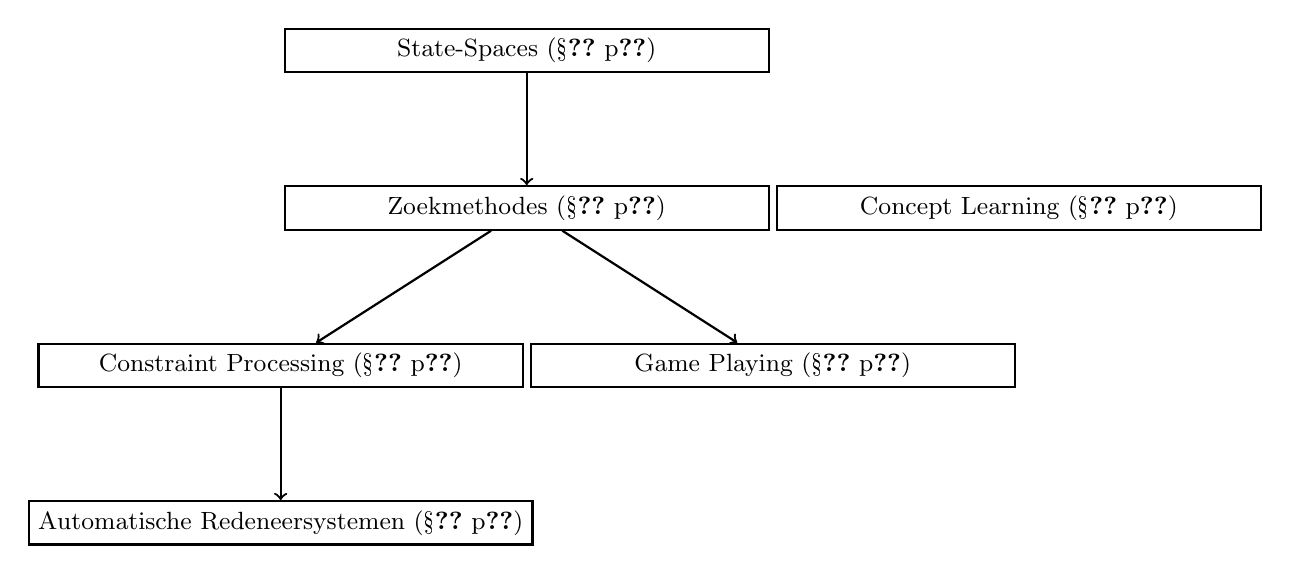
\begin{tikzpicture}[topict/.style={shape=rectangle,draw=black,thick,minimum width=6.15 cm},influences/.style={thick,->}]
\node[topict] (S) at (0,0) {\small State-Spaces (\S\ref{s:stateSpaces} p\pageref{s:stateSpaces})};
\node[topict] (Z) at (0,-2) {\small Zoekmethodes (\S\ref{s:searchMethods} p\pageref{s:searchMethods})};
\node[topict] (CL) at (6.25,-2) {\small Concept Learning (\S\ref{s:conceptLearning} p\pageref{s:conceptLearning})};
\node[topict] (CP) at (-3.125,-4) {\small Constraint Processing (\S\ref{s:constraintProcessing} p\pageref{s:constraintProcessing})};
\node[topict] (G) at (3.125,-4) {\small Game Playing (\S\ref{s:gamePlaying} p\pageref{s:gamePlaying})};
\node[topict] (A) at (-3.125,-6) {\small Automatische Redeneersystemen (\S\ref{s:automaticReasoning} p\pageref{s:automaticReasoning})};
\draw[influences] (S) -- (Z);
\draw[influences] (Z) -- (CP);
\draw[influences] (Z) -- (G);
\draw[influences] (CP) -- (A);
\end{tikzpicture}
\caption{Indeling en afhankelijkheden van deze cursus}
\label{fig:partsAndDependenciesOfCourse}
\end{figure}

\section*{Layout en Stijl}
\chapterquote{De eerste eigenschap van stijl is helderheid.}{Aristoteles, Grieks filosoof (384 v.C. - 322 v.C.)}
Naast een cursus met een goeie inhoud, is ook de opmaak een belangrijk aspect. Om het leerproces zoveel mogelijk te bevorderen heeft de auteur volgende overwegingen gemaakt wat betreft de layout.
\paragraph{}
Alle pagina's zijn afdrukbaar met een zwart-wit printer. Dit drukt de eventuele kosten bij een afdruk van deze cursus. Bovendien verhoogt dit de leesbaarheid bij kleurenblindheid. Op het einde van de cursus staan enkele samenvattende schema's waar ook versies in kleur van beschikbaar zijn.
\paragraph{}
Deze cursus wordt ge\"illustreerd met talloze afbeeldingen. Deze zijn allemaal tot stand gekomen met het grafisch pakket Ti\textit{k}Z\footnote{TikZ ist kein Zeichenprogramm}. Alle afbeeldingen zijn bijgevolg vectorieel.
\begin{leftbar}
In elk hoofdstuk worden de technieken besproken aan de hand van een leidend voorbeeld. Tekst gerelateerd aan het leidend voorbeeld wordt zoals hier weergegeven met een zwarte rand. Indien de techniek in kwestie duidelijk is, mogen deze stukken overgeslagen worden.
\end{leftbar}
\paragraph{}
Belangrijke \termenlayout{terminologie} wordt in het vetjes zonder schreven\footnote{De zogenoemde ``pootjes'' die letters krijgen. (Engels: serifs)} gezet. Deze terminologie komt ook in de index achteraan de cursus. Deze index verwijst dus niet noodzakelijk naar de definities van de termen. Maar naar de pagina waar de term in kwestie voor het eerst voorkomt.
\begin{figure}[H]
\centering

\begin{tikzpicture}
\draw[black!34] (0,0) node[scale=12]{\Huge{$\varphi$}};
\end{tikzpicture}
\end{figure}

\section{State-Spaces}
\label{s:stateSpaces}
\chapterquote{Voor elke toestand, hoe moeilijk ook is er een uitweg. Het komt er alleen op aan een besluit te nemen.}{Leo Tolstoy, Russisch romanschrijver (1828-1910)}
\subsection{Leidend Voorbeeld: Missionaries \& Cannibals}
\begin{leftbar}
Als leidend voorbeeld voor dit eerste hoofdstuk opteren we voor het Missionaries \& Cannibals probleem. Dit probleem kunnen we als volgt beschrijven: we beschouwen twee oevers, aan één kant staan drie missionarissen en drie kannibalen. Aan de oever ligt ook een boot, deze kan maximum twee personen (kannibalen of missionarissen) tegelijk overzetten. De boot kan alleen de andere oever bereiken indien minstens één persoon zich in de boot bevindt. Het is de bedoeling dat zowel de drie missionarissen als de kannibalen de andere oever bereiken. Indien echter aan een oever meer kannibalen dan missionarissen staan, verliezen deze de macht over de kannibalen, en worden ze opgegeten, en is het spel ten einde. Dit is schematisch weergegeven op figuur \ref{fig:missionariesAndCannibals}.
\end{leftbar}
\begin{figure}[htb]
\centering
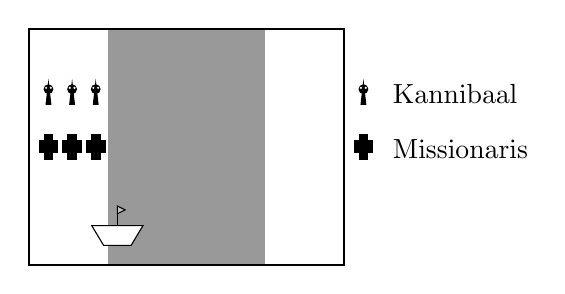
\begin{tikzpicture}
\def\ss{1.3247};
\def\cw{0.25};
\def\ch{\cw*\ss};
\fill[gray!80] (-1,-1.5) rectangle (1,1.5);
\draw[thick] (-2,-1.5) rectangle (2,1.5);
\filldraw[fill=white,draw=black] (-1.2,-1) -- (-0.55,-1) -- (-0.7,-1.25) -- (-1.05,-1.25) -- cycle;
\filldraw[fill=gray!50,draw=black] (-0.875,-0.85) -- (-0.875,-0.75) -- (-0.775,-.8) -- cycle;
\draw (-0.875,-1) -- (-0.875,-0.85);
\foreach\x in {0,0.3,0.6} {
  \fill (-1.75-0.25*\cw+\x,-0.5*\ch) rectangle (-1.75+0.25*\cw+\x,0.5*\ch);
  \fill (-1.75-0.5*\cw+\x,-0.25*\ch) rectangle (-1.75+0.5*\cw+\x,0.25*\ch);
  \fill (-1.75-0.15*\cw+\x,0.7-0.5*\ch) -- (-1.75+\x,0.7+0.5*\ch) -- (-1.75+0.15*\cw+\x,0.7-0.5*\ch) -- cycle;
  \fill (-1.75+\x,0.7+0.1*\ch) circle(0.25*\cw);
  \fill[white] (-1.78+\x,0.7+0.15*\ch) circle(0.06125*\cw);
  \fill[white] (-1.72+\x,0.7+0.15*\ch) circle(0.06125*\cw);
}
\fill (-1.75-0.25*\cw+4,-0.5*\ch) rectangle (-1.75+0.25*\cw+4,0.5*\ch);
\fill (-1.75-0.5*\cw+4,-0.25*\ch) rectangle (-1.75+0.5*\cw+4,0.25*\ch);
\fill (-1.75-0.15*\cw+4,0.7-0.5*\ch) -- (-1.75+4,0.7+0.5*\ch) -- (-1.75+0.15*\cw+4,0.7-0.5*\ch) -- cycle;
\fill (-1.75+4,0.7+0.1*\ch) circle(0.25*\cw);
\fill[white] (-1.78+4,0.7+0.15*\ch) circle(0.06125*\cw);
\fill[white] (-1.72+4,0.7+0.15*\ch) circle(0.06125*\cw);
\draw (2.5,0.7-0.1*\ch) node[anchor=west] {Kannibaal};
\draw (2.5,-0.1*\ch) node[anchor=west] {Missionaris};
\end{tikzpicture}
\caption{Begintoestand van het Missionaries \& Cannibals probleem}
\label{fig:missionariesAndCannibals}
\end{figure}
\subsection{Wat is een State-space?}
Een \termen{state-space} is de verzameling van de verschillende staten (toestanden) waarin een probleem zich kan bevinden, waarbij de staat deterministisch en ondubbelzinnig uitgedrukt wordt. Daarnaast bevat een state-space ook een set \termen{productieregels}: condities om van de ene staat van het probleem naar een andere te gaan. Verder bezit een state-space ook een set \termen{begin sta(a)t(en)}, en een set voorwaarden waarbij het \termen{doel} is bereikt (we het probleem dus opgelost hebben).
\paragraph{}
\begin{leftbar}
Hoe zouden we nu het Missionaries \& Cannibals probleem kunnen omzetten naar een statespace? Het enige wat we eigenlijk moeten weten is hoeveel missionarissen en cannibalen er aan één van de twee oevers staan, en aan welke oever de boot ligt. Daarom introduceren we een notatie die er als volgt uit ziet: $\left\langle M,K,B\right\rangle$ hierbij stellen $M$ het aantal missionarissen, en $K$ het aantal kannibalen voor op de linkeroever. En schrijven we voor $B$, $l$ indien de boot zich op de linkeroever, en $r$ indien de boot zich op de rechteroever bevindt. De begintoestand noteren we dus als $\left\langle3,3,l\right\rangle$. Het doel is logischerwijs: $\left\langle0,0,r\right\rangle$.
\paragraph{}
Zoals reeds eerder vermeld, is dit probleem gebonden aan enkele voorwaarden. Zo mogen er nooit meer kannibalen dan missionarissen op één van de oevers aanwezig zijn, tenzij er zich geen missionarissen op deze oever bevinden. Dit vertaald zich naar twee regels die we hieronder beschrijven:
\begin{equation}
\left\langle M,K,B\right\rangle\mbox{ is geldig}\Leftrightarrow\left\{
\begin{array}{cl}
M=0\vee M\geq K&\mbox{\{Linker oever\}}\\
\wedge\\
M=3\vee M\leq K&\mbox{\{Rechter oever\}}
\end{array}\right.
\end{equation}
\paragraph{}
Welke productieregels definiëren we? Indien de boot links staat dienen we minstens één en maximum twee personen over te zetten. Omgekeerd indien de boot aan de rechter oever ligt, dienen we één of twee personen aan de linkerover toe te voegen. Indien we deze regels formaliseren, bekomen we volgende regels:
\begin{equation}
\left\{\begin{array}{rcl|l}
\left\langle M,K,l\right\rangle&\Rightarrow&\left\langle M-\delta_m,K-\delta_k,r\right\rangle&\delta_m,\delta_k\in\left\{0,1,2\right\}\wedge1\leq\delta_m+\delta_k\leq 2\\
\left\langle M,K,r\right\rangle&\Rightarrow&\left\langle M+\delta_m,K+\delta_k,l\right\rangle&\delta_m,\delta_k\in\left\{0,1,2\right\}\wedge1\leq\delta_m+\delta_k\leq 2\\
\end{array}\right.
\end{equation}
\end{leftbar}
\subsection{Wat zijn de keuzes bij een State-space?}
\label{ss:stateSpaceTradeOffs}
Er zijn verschillende keuzes te maken:
\begin{itemize}
 \item Welke regel passen we eerst toe (proberen we eerst uit)
 \item Zoeken we in een boom of een graaf
 \item Zijn we op zoek naar de optimale oplossing, of is een oplossing voldoende
 \item Kunnen we het probleem opdelen in verschillende deelproblemen
 \item Zoeken we vooruit of achteruit
\end{itemize}
\paragraph{}
Indien we voor een optimale oplossing kiezen moeten we bijhouden wat de geaccumuleerde kost (zie \ref{ss:optimalSearch}) precies inhoud.
\paragraph{}
Indien we een keuze maken tussen \termen{voorwaarts redeneren} of \termen{achterwaarts redeneren}, moeten we vooral kijken naar de volgende criteria:
\begin{itemize}
 \item Zijn de regels achterwaarts te construeren: (bij schaken kan je niet achteruit denken)
 \item \termen{Branching factor}: het gemiddelde aantal staten die direct afgeleid kan worden uit een staat.
 \item Aantal begintoestanden ten opzichte van het aantal eindtoestanden
 \item Een achterwaartse redenering kan meestal meer zijn keuzes verklaren
\end{itemize}
Een andere mogelijkheid is \termen{Middle-out reasoning} waarbij vanuit een bepaalde staat naar het doel en een begin gegraven wordt.
\paragraph{}
\begin{leftbar}
Het is duidelijk dat de het Missionaries \& Cannibals probleem een graaf is, immers kunnen we indien we een bepaalde transactie gedaan hebben, telkens deze ongedaan maken door de overgezette personen terug over te zetten. Op zich zijn we niet op zoek naar de kortste oplossing. We kunnen echter wel oplossingen genereren die heel veel redundant werk doen (door bijvoorbeeld een aantal keer op stappen terug te keren). Omdat dit probleem relatief simpel is, is het niet verder op te delen. We kunnen het probleem ook trachtten op te lossen door achterwaarts vanuit de oplossing te redeneren. Maar deze oplossing is eigenlijk volledig identiek. Op figuur \ref{fig:missionariesAndCannibalsGraph} wordt de graaf weergegeven die alle toestanden van het probleem weergeeft.
\end{leftbar}
\begin{figure}[htb]
\centering
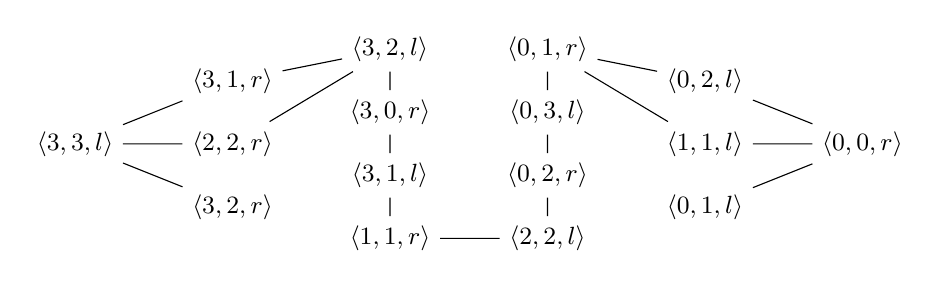
\begin{tikzpicture}
\def\dx{2};
\def\dy{-0.8};
\node (S33l) at (0,0) {\small$\left\langle 3,3,l\right\rangle$};
\node (S32r) at (\dx,\dy) {\small$\left\langle 3,2,r\right\rangle$};
\node (S22r) at (\dx,0) {\small$\left\langle 2,2,r\right\rangle$};
\node (S31r) at (\dx,-\dy) {\small$\left\langle 3,1,r\right\rangle$};
\node (S32l) at (2*\dx,-1.5*\dy) {\small$\left\langle 3,2,l\right\rangle$};
\node (S30r) at (2*\dx,-0.5*\dy) {\small$\left\langle 3,0,r\right\rangle$};
\node (S31l) at (2*\dx,0.5*\dy) {\small$\left\langle 3,1,l\right\rangle$};
\node (S11r) at (2*\dx,1.5*\dy) {\small$\left\langle 1,1,r\right\rangle$};
\node (S22l) at (3*\dx,1.5*\dy) {\small$\left\langle 2,2,l\right\rangle$};
\node (S02r) at (3*\dx,0.5*\dy) {\small$\left\langle 0,2,r\right\rangle$};
\node (S03l) at (3*\dx,-0.5*\dy) {\small$\left\langle 0,3,l\right\rangle$};
\node (S01r) at (3*\dx,-1.5*\dy) {\small$\left\langle 0,1,r\right\rangle$};
\node (S01l) at (4*\dx,\dy) {\small$\left\langle 0,1,l\right\rangle$};
\node (S11l) at (4*\dx,0) {\small$\left\langle 1,1,l\right\rangle$};
\node (S02l) at (4*\dx,-\dy) {\small$\left\langle 0,2,l\right\rangle$};
\node (S00r) at (5*\dx,0) {\small$\left\langle 0,0,r\right\rangle$};
\draw (S33l) -- (S32r);
\draw (S33l) -- (S22r) -- (S32l);
\draw (S33l) -- (S31r) -- (S32l) -- (S30r) -- (S31l) -- (S11r) -- (S22l) -- (S02r) -- (S03l) -- (S01r) -- (S02l) -- (S00r);
\draw (S01r) -- (S11l) -- (S00r);
\draw (S01l) -- (S00r);
\end{tikzpicture}
\caption{Graaf van de verschillende toestanden}
\label{fig:missionariesAndCannibalsGraph}
\end{figure}

\section{Zoekmethodes}
\label{s:searchMethods}
\chapterquote{Toen ik moe was van zoeken, leerde ik vinden.}{Friedrich Nietzsche, Duits dichter en filosoof (1844-1900)}
Indien we een state-space gebouwd hebben, kunnen we vervolgens een algoritme ontwikkelen die door deze state-space zoekt naar een oplossing. Hiervoor bestaan er verschillende methodes die kunnen gebruikt worden: De \termen{basic search methods}.
\paragraph{Evaluatie-criteria}
We kunnen een zoekmethode evalueren op volgende criteria:
\begin{itemize}
 \item \termen{Completeness}: vindt het algoritme altijd een oplossing (indien er een oplossing bestaat)
 \item \termen{Speed}: de worst-case tijdscomplexiteit
 \item \termen{Memory}: de worst-case geheugencomplexiteit
 \item \termen{Optimaliteit}: zoeken we de optimale oplossing, of is \'e\'en oplossing voldoende
\end{itemize}
Voor complexiteitsanalyses zullen we gebruikmaken van onderstaande parameters:
\begin{itemize}
 \item $d$: de diepte van de boom
 \item $b$: de vertakkingsfactor
 \item $m$: de diepte van de minst diepe oplossing
 \item $\delta$: de kleinste kost tussen twee staten (zie \ref{ss:optimalSearch})
\end{itemize}
\subsection{Leidend Voorbeeld: Wegenplan}
\begin{leftbar}
Doorheen deze sectie zullen we vaak concepten verduidelijken met behulp van een voorbeeld. Dit voorbeeld wordt hieronder kort toegelicht. Het betreft een sterk vereenvoudigd wegenplan. Hierbij willen we vanuit $S$ (de begintoestand), $G$ (het doel) bereiken. We gaan er vanuit dat er slechts 9 steden bestaan: $A$ (Antwerpen), $B$ (Brussel), $C$ (Charleroi), $D$ (Durbuy), $E$ (Eeklo), $F$ (Fosses-la-Ville), $G$ (Geel), $H$ (Hoei) en $S$ (Sint-Niklaas). Verder bestaan er alleen wegen die tussen twee steden lopen met een bepaalde afstand in kilometer. Dit wordt weergegeven op figuur \ref{fig:searchMapCity}.
\end{leftbar}
\begin{figure}[htb]
\centering
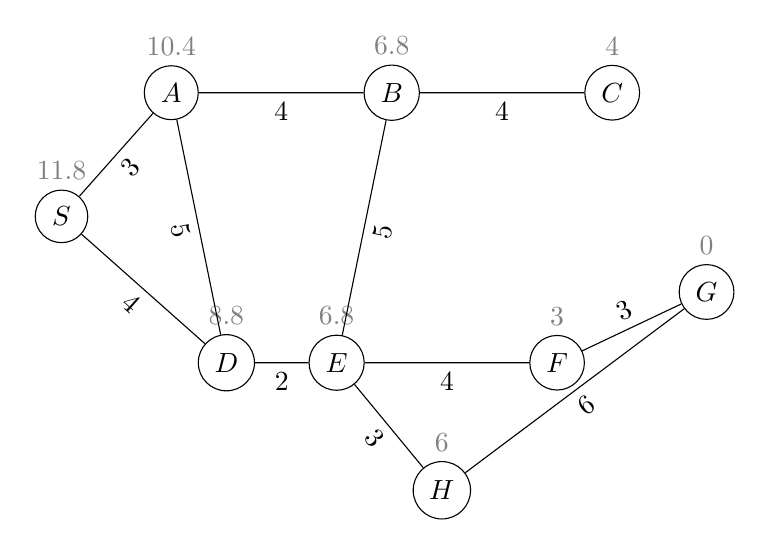
\begin{tikzpicture}[scale=0.7,city/.style={shape=circle,draw=black},dist/.style={sloped,below},heur/.style={gray,anchor=south}]
\def\sqrttf{4.898979486};
\def\sqrts{2.449489743};
\def\xs{-24*\sqrts/25-16/25};
\def\ys{32*\sqrts/25-12/25};
\def\xg{8.71151};
\def\yg{1.28363};
\def\xh{3.90957};
\def\yh{-2.31377};
\node[city] (S) at (\xs,\ys) {$S$};
\node[city] (A) at (-1,\sqrttf) {$A$};
\node[city] (B) at (3,\sqrttf) {$B$};
\node[city] (C) at (7,\sqrttf) {$C$};
\node[city] (D) at (0,0) {$D$};
\node[city] (E) at (2,0) {$E$};
\node[city] (F) at (6,0) {$F$};
\node[city] (G) at (\xg,\yg) {$G$};
\node[city] (H) at (\xh,\yh) {$H$};
\node[heur] (Sh) at (S.north) {$11.8$};
\node[heur] (Ah) at (A.north) {$10.4$};
\node[heur] (Bh) at (B.north) {$6.8$};
\node[heur] (Ch) at (C.north) {$4$};
\node[heur] (Dh) at (D.north) {$8.8$};
\node[heur] (Eh) at (E.north) {$6.8$};
\node[heur] (Fh) at (F.north) {$3$};
\node[heur] (Gh) at (G.north) {$0$};
\node[heur] (Hh) at (H.north) {$6$};
\draw (S) to node[dist]{3} (A) to node[dist]{5} (D) to node[dist]{2} (E) to node[dist]{5} (B) to node[dist]{4} (C);
\draw (E) to node[dist]{4} (F) to node[dist,above]{3} (G);
\draw (E) to node[dist]{3} (H) to node[dist]{6} (G);
\draw (S) to node[dist]{4} (D);
\draw (A) to node[dist]{4} (B);
\end{tikzpicture}
\caption{Voorstelling van een door ons beschouwd wegenplan}
\label{fig:searchMapCity}
\end{figure}
\begin{leftbar}
Als overgangsregels beschouwen we iedere weg naar iedere stad die we tot dan toe nog niet bezocht hebben. Vanuit $S$ kunnen we dus naar twee andere toestanden: $A$ en $D$. Indien we vervolgens verder de productieregels op deze toestanden toepassen, bekomen we een boom zoals op figuur \ref{fig:searchTreeCity}.
\end{leftbar}
\begin{figure}[htb]
\centering
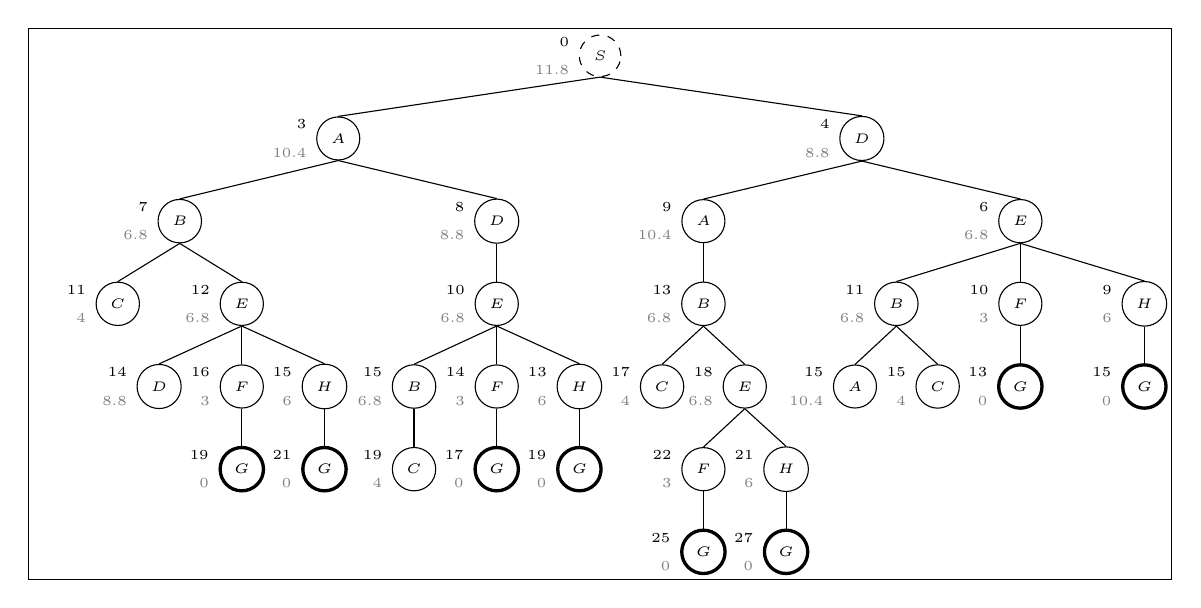
\begin{tikzpicture}[scale=1.4,city/.style={shape=circle,draw=black},costc/.style={anchor=south east},heurh/.style={anchor=north east,gray},cityG/.style={city,very thick},cityM/.style={city,fill=gray}]
\def\dy{-0.75};
\def\dxa{4.75};
\def\dxb{2.875};
\def\dxc{1.125};
\def\dxd{0.75};
\def\dxe{0.75};

\draw (-0.5*\dxa-0.5*\dxb-\dxc-0.25,0.25) rectangle (0.5*\dxa+0.5*\dxb+\dxc+0.25,6*\dy-0.25);

\node[city,dashed] (S) at (0,0) {\tiny $S$};
\node[costc] (Sc) at (S.west) {\tiny 0};
\node[heurh] (Sh) at (S.west) {\tiny 11.8};

\node[city] (A) at (-0.5*\dxa,\dy) {\tiny $A$};
\node[costc] (Ac) at (A.west) {\tiny 3};
\node[heurh] (Ah) at (A.west) {\tiny 10.4};
\draw (S.south) -- (A.north);
\node[city] (D) at (0.5*\dxa,\dy) {\tiny $D$};
\node[costc] (Dc) at (D.west) {\tiny 4};
\node[heurh] (Dh) at (D.west) {\tiny 8.8};
\draw (S.south) -- (D.north);

\node[city] (B) at (-0.5*\dxa-0.5*\dxb,2*\dy) {\tiny $B$};
\node[costc] (Bc) at (B.west) {\tiny 7};
\node[heurh] (Bh) at (B.west) {\tiny 6.8};
\draw (A.south) -- (B.north);
\node[city] (D2) at (-0.5*\dxa+0.5*\dxb,2*\dy) {\tiny $D$};
\node[costc] (D2c) at (D2.west) {\tiny 8};
\node[heurh] (D2h) at (D2.west) {\tiny 8.8};
\draw (A.south) -- (D2.north);
\node[city] (A2) at (0.5*\dxa-0.5*\dxb,2*\dy) {\tiny $A$};
\node[costc] (A2c) at (A2.west) {\tiny 9};
\node[heurh] (A2h) at (A2.west) {\tiny 10.4};
\draw (D.south) -- (A2.north);
\node[city] (E) at (0.5*\dxa+0.5*\dxb,2*\dy) {\tiny $E$};
\node[costc] (Ec) at (E.west) {\tiny 6};
\node[heurh] (Eh) at (E.west) {\tiny 6.8};
\draw (D.south) -- (E.north);

\node[city] (C) at (-0.5*\dxa-0.5*\dxb-0.5*\dxc,3*\dy) {\tiny $C$};
\node[costc] (Cc) at (C.west) {\tiny 11};
\node[heurh] (Ch) at (C.west) {\tiny 4};
\draw (B.south) -- (C.north);
\node[city] (E2) at (-0.5*\dxa-0.5*\dxb+0.5*\dxc,3*\dy) {\tiny $E$};
\node[costc] (E2c) at (E2.west) {\tiny 12};
\node[heurh] (E2h) at (E2.west) {\tiny 6.8};
\draw (B.south) -- (E2.north);
\node[city] (E3) at (-0.5*\dxa+0.5*\dxb,3*\dy) {\tiny $E$};
\node[costc] (E3c) at (E3.west) {\tiny 10};
\node[heurh] (E3h) at (E3.west) {\tiny 6.8};
\draw (D2.south) -- (E3.north);
\node[city] (B2) at (0.5*\dxa-0.5*\dxb,3*\dy) {\tiny $B$};
\node[costc] (B2c) at (B2.west) {\tiny 13};
\node[heurh] (B2h) at (B2.west) {\tiny 6.8};
\draw (A2.south) -- (B2.north);
\node[city] (B3) at (0.5*\dxa+0.5*\dxb-\dxc,3*\dy) {\tiny $B$};
\node[costc] (B3c) at (B3.west) {\tiny 11};
\node[heurh] (B3h) at (B3.west) {\tiny 6.8};
\draw (E.south) -- (B3.north);
\node[city] (F) at (0.5*\dxa+0.5*\dxb,3*\dy) {\tiny $F$};
\node[costc] (Fc) at (F.west) {\tiny 10};
\node[heurh] (Fh) at (F.west) {\tiny 3};
\draw (E.south) -- (F.north);
\node[city] (H) at (0.5*\dxa+0.5*\dxb+\dxc,3*\dy) {\tiny $H$};
\node[costc] (Hc) at (H.west) {\tiny 9};
\node[heurh] (Hh) at (H.west) {\tiny 6};
\draw (E.south) -- (H.north);

\node[city] (D3) at (-0.5*\dxa-0.5*\dxb+0.5*\dxc-\dxd,4*\dy) {\tiny $D$};
\node[costc] (D3c) at (D3.west) {\tiny 14};
\node[heurh] (D3h) at (D3.west) {\tiny 8.8};
\draw (E2.south) -- (D3.north);
\node[city] (F2) at (-0.5*\dxa-0.5*\dxb+0.5*\dxc,4*\dy) {\tiny $F$};
\node[costc] (F2c) at (F2.west) {\tiny 16};
\node[heurh] (F2h) at (F2.west) {\tiny 3};
\draw (E2.south) -- (F2.north);
\node[city] (H2) at (-0.5*\dxa-0.5*\dxb+0.5*\dxc+\dxd,4*\dy) {\tiny $H$};
\node[costc] (H2c) at (H2.west) {\tiny 15};
\node[heurh] (H2h) at (H2.west) {\tiny 6};
\draw (E2.south) -- (H2.north);
\node[city] (B4) at (-0.5*\dxa+0.5*\dxb-\dxd,4*\dy) {\tiny $B$};
\node[costc] (B4c) at (B4.west) {\tiny 15};
\node[heurh] (B4h) at (B4.west) {\tiny 6.8};
\draw (E3.south) -- (B4.north);
\node[city] (F3) at (-0.5*\dxa+0.5*\dxb,4*\dy) {\tiny $F$};
\node[costc] (F3c) at (F3.west) {\tiny 14};
\node[heurh] (F3h) at (F3.west) {\tiny 3};
\draw (E3.south) -- (F3.north);
\node[city] (H3) at (-0.5*\dxa+0.5*\dxb+\dxd,4*\dy) {\tiny $H$};
\node[costc] (H3c) at (H3.west) {\tiny 13};
\node[heurh] (H3h) at (H3.west) {\tiny 6};
\draw (E3.south) -- (H3.north);
\node[city] (C2) at (0.5*\dxa-0.5*\dxb-0.5*\dxd,4*\dy) {\tiny $C$};
\node[costc] (C2c) at (C2.west) {\tiny 17};
\node[heurh] (C2h) at (C2.west) {\tiny 4};
\draw (B2.south) -- (C2.north);
\node[city] (E4) at (0.5*\dxa-0.5*\dxb+0.5*\dxd,4*\dy) {\tiny $E$};
\node[costc] (E4c) at (E4.west) {\tiny 18};
\node[heurh] (E4h) at (E4.west) {\tiny 6.8};
\draw (B2.south) -- (E4.north);
\node[city] (A3) at (0.5*\dxa+0.5*\dxb-\dxc-0.5*\dxd,4*\dy) {\tiny $A$};
\node[costc] (A3c) at (A3.west) {\tiny 15};
\node[heurh] (A3h) at (A3.west) {\tiny 10.4};
\draw (B3.south) -- (A3.north);
\node[city] (C3) at (0.5*\dxa+0.5*\dxb-\dxc+0.5*\dxd,4*\dy) {\tiny $C$};
\node[costc] (C3c) at (C3.west) {\tiny 15};
\node[heurh] (C3h) at (C3.west) {\tiny 4};
\draw (B3.south) -- (C3.north);
\node[cityG] (G) at (0.5*\dxa+0.5*\dxb,4*\dy) {\tiny $G$};
\node[costc] (Gc) at (G.west) {\tiny 13};
\node[heurh] (Gh) at (G.west) {\tiny 0};
\draw (F.south) -- (G.north);
\node[cityG] (G2) at (0.5*\dxa+0.5*\dxb+\dxc,4*\dy) {\tiny $G$};
\node[costc] (G2c) at (G2.west) {\tiny 15};
\node[heurh] (G2h) at (G2.west) {\tiny 0};
\draw (H.south) -- (G2.north);

\node[cityG] (G3) at (-0.5*\dxa-0.5*\dxb+0.5*\dxc,5*\dy) {\tiny $G$};
\node[costc] (G3c) at (G3.west) {\tiny 19};
\node[heurh] (G3h) at (G3.west) {\tiny 0};
\draw (F2.south) -- (G3.north);
\node[cityG] (G4) at (-0.5*\dxa-0.5*\dxb+0.5*\dxc+\dxd,5*\dy) {\tiny $G$};
\node[costc] (G4c) at (G4.west) {\tiny 21};
\node[heurh] (G4h) at (G4.west) {\tiny 0};
\draw (H2.south) -- (G4.north);
\node[city] (C4) at (-0.5*\dxa+0.5*\dxb-\dxd,5*\dy) {\tiny $C$};
\node[costc] (C4c) at (C4.west) {\tiny 19};
\node[heurh] (C4h) at (C4.west) {\tiny 4};
\draw (B4.south) -- (C4.north);
\node[cityG] (G5) at (-0.5*\dxa+0.5*\dxb,5*\dy) {\tiny $G$};
\node[costc] (G5c) at (G5.west) {\tiny 17};
\node[heurh] (G5h) at (G5.west) {\tiny 0};
\draw (F3.south) -- (G5.north);
\node[cityG] (G6) at (-0.5*\dxa+0.5*\dxb+\dxd,5*\dy) {\tiny $G$};
\node[costc] (G6c) at (G6.west) {\tiny 19};
\node[heurh] (G6h) at (G6.west) {\tiny 0};
\draw (H3.south) -- (G6.north);
\node[city] (F4) at (0.5*\dxa-0.5*\dxb+0.5*\dxd-0.5*\dxe,5*\dy) {\tiny $F$};
\node[costc] (F4c) at (F4.west) {\tiny 22};
\node[heurh] (F4h) at (F4.west) {\tiny 3};
\draw (E4.south) -- (F4.north);
\node[city] (H4) at (0.5*\dxa-0.5*\dxb+0.5*\dxd+0.5*\dxe,5*\dy) {\tiny $H$};
\node[costc] (H4c) at (H4.west) {\tiny 21};
\node[heurh] (H4h) at (H4.west) {\tiny 6};
\draw (E4.south) -- (H4.north);

\node[cityG] (G7) at (0.5*\dxa-0.5*\dxb+0.5*\dxd-0.5*\dxe,6*\dy) {\tiny $G$};
\node[costc] (G7c) at (G7.west) {\tiny 25};
\node[heurh] (G7h) at (G7.west) {\tiny 0};
\draw (F4.south) -- (G7.north);
\node[cityG] (G8) at (0.5*\dxa-0.5*\dxb+0.5*\dxd+0.5*\dxe,6*\dy) {\tiny $G$};
\node[costc] (G8c) at (G8.west) {\tiny 27};
\node[heurh] (G8h) at (G8.west) {\tiny 0};
\draw (H4.south) -- (G8.north);
\end{tikzpicture}
\caption{Zoekboom van het wegenplan}
\label{fig:searchTreeCity}
\end{figure}
\begin{leftbar}
Als heuristiek (zie \ref{sss:heuristicFunction}) nemen we tot slot de afstand in vogelvlucht tussen de stad in kwestie, en $G$ zelf. Deze wordt in het grijs op het wegenplan aangegeven. We zullen in deze sectie heel wat zoekalgoritmen uitvoeren op deze boom, om zo de concrete werking te verduidelijken. Deze afbeeldingen staan niet in de tekst zelf, maar staan in \ref{ss:cityFigures} op pagina \pageref{ss:cityFigures}.
\end{leftbar}
\subsection{Blind Search Methods}
Indien we geen specifieke kennis over het probleem hebben, of deze te complex/lastig is om te formuleren kunnen we een \termen{Blind Search Method} gebruiken. Het is evident dat zoeken zonder probleemgerelateerde informatie ineffici\"ent is. Bij deze methodes zijn we ook niet ge\"interesseerd in de optimale oplossing.
\subsubsection{Depth-First Search}
Bij \termen{Depth-First Search} of \termen{Diepte-eerst zoeken} volgen we een bepaalde productieregel vanaf de begintoestand. Vervolgens blijven we deze regel recursief toepassen tot we vast zitten. Indien we een doel gevonden hebben is het algoritme ten einde. Indien het niet het doel is, zal het algoritme de laatste productieregel ongedaan maken en een andere in de plaats stellen. Indien er geen ongebruikte regels meer voor handen zijn maken we de regels daarvoor ongedaan tot we terug een regel kunnen kiezen. Een andere naam hiervoor is \termen{Chronological Backtracking}. Deze zoekmethode wordt ge\"illustreerd in \algref{alg:depthFirst}. We voorkomen dat we in een lus terechtkomen (indien de productieregel dit toelaten) door telkens we een toestand genereren te controleren of \'e\'en van zijn voorouders identiek aan die toestand is. Indien dit zo is, zullen we die toestand niet meer verder evalueren. Dit systeem noemen we \termen{Loopdetectie}.
\begin{algorithm}[htb]
\caption{Depth-First zoekalgoritme}
\label{alg:depthFirst}
\begin{algorithmic}[1]
\STATE $\queue\leftarrow\mbox{Path containing the root}$
\WHILE{$\notempty{\queue}\wedge\neg\goalreached{\queue}$}
\STATE $r\leftarrow\dequeue{\queue}$
\STATE $R\leftarrow\createnewpaths{r}$
\STATE $\removeloops{R}$
\STATE $\enqueuefront{\queue,R}$
\ENDWHILE
\IF{$\goalreached{\queue}$}
\RETURN $\success$
\ELSE
\RETURN $\failure$
\ENDIF
\end{algorithmic}
\end{algorithm}
\paragraph{Complexiteiten}
We zullen nu de tijd- en geheugencomplexiteit voor Depth-First analyseren. Hierbij zullen we systemen zoals het loopdetectie systeem buiten beschouwing laten. We gaan er dus vanuit dat we een pad analyseren in \bigoh{1}. Dit is uiteraard niet het geval, en zal in andere algoritmes zelfs oplopen tot lange procedures. We zijn dus meer ge\"interesseerd in het aantal maal we de while-lus uitvoeren, en beschouwen dit als tijdscomplexiteit. 
\paragraph{}
Indien we dit toepassen op Depth-First stellen we vast dat we een tijdscomplexiteit van \bigoh{b^d} uitkomen. Vrij vertaald betekent dit dus dat we de volledige boom doorlopen. Dit is te beargumenteren: stel dat de oplossing zich in de meest rechtse tak bevindt. In dat geval, zal Depth-First eerst alle andere paden van links naar rechts doorlopen. Het maakt niet zoveel uit op welke diepte de oplossing zich bevindt (indien niet onmiddellijk onder de wortel). Deze eigenschap kan ook de compleetheid van het algoritme ook in gevaar brengen. Indien we met een oneindig diepe boom te maken hebben. Waarbij we telkens verder op een bepaalde knoop kunnen produceren, zal het algoritme nooit stoppen. We moeten dus over productieregels beschikken die vroeg of laat ieder pad doen stoppen, om dit algoritme volledig te doen werken.
\paragraph{}
Het geheugengebruik van Depth-First is beter. Op ieder niveau is op ieder moment hooguit \'e\'en knoop ge\"expandeert, bijgevolg zitten er in de $\queue$ hooguit \bigoh{b\cdot d} knopen. Namelijk per diepte $b$ verschillende knopen.	
\paragraph{}
Indien we dit samenvatten bekomen we volgende criteria:
\begin{center}
\begin{tabular}{ll}
\textbf{Compleet}:&Ja, indien geen oneindig diepe boom\\
\textbf{Snelheid}:&\bigoh{b^d}\\
\textbf{Geheugen}:&\bigoh{b\cdot d}\\
\textbf{Optimaal}:&Nee
\end{tabular}
\end{center}
\begin{leftbar}
We illustreren de werking van dit algoritme op het wegenplan in figuur \ref{fig:depthFirstCity} op pagina \pageref{fig:depthFirstCity}.
\end{leftbar}
\subsubsection{Breadth-First Search}
Bij \termen{Breadth-First Search} of de \termen{Breedte-eerst zoeken} zoekmethode wordt een laag aan oplossingen afgewerkt alvorens er een nieuwe laag wordt bekeken. Concreet betekent dit dus dat de kinderen van een ge\"evalueerde knoop achteraan in een wachtrij geplaatst worden, en dus pas behandeld worden wanneer alle andere knopen van dezelfde boom toegevoegd zijn. Dit wordt ge\"illustreerd in \algref{alg:breadthFirst}.
\begin{algorithm}[htb]
\caption{Breadth-First zoekalgoritme}
\label{alg:breadthFirst}
\begin{algorithmic}[1]
\STATE $\queue\leftarrow\mbox{Path containing the root}$
\WHILE{$\notempty{\queue}\wedge\neg\goalreached{\queue}$}
\STATE $r\leftarrow\dequeue{\queue}$
\STATE $R\leftarrow\createnewpaths{r}$
\STATE $\removeloops{R}$
\STATE $\enqueueback{\queue,R}$
\ENDWHILE
\IF{$\goalreached{\queue}$}
\RETURN $\success$
\ELSE
\RETURN $\failure$
\ENDIF
\end{algorithmic}
\end{algorithm}
\paragraph{Complexiteiten}
In tijdscomplexiteit is een breedte eerst benadering in de meeste gevallen beter. Het algoritme zal immers alleen de boom expanderen tot de diepte waar een doel zich bevindt. De boom die we bekomen tot een diepte $m$ telt \bigoh{b^m} knopen. Bijgevolg hebben we dus ook \bigoh{b^{m-1}} evaluaties gedaan. Of eenvoudiger \bigoh{b^m}. Een ander voordeel van een Breedte-Eerst benadering is dat ook oneindig diepe bomen ge\"evalueerd kunnen worden. Bovendien zal het algoritme als oplossing een pad teruggeven met het minimale aantal stappen om tot een oplossing te komen (niet te verwarren met goedkoopste bij optimaal zoeken, het is niet omdat we het minste aantal steden passeren, dat we ook het minste kilometers afleggen).
\paragraph{}
De ommezijde van deze medaille is dat het geheugen erg oneffici\"ent gebruikt wordt. Dit moet immers telkens alle paden bijhouden op een diepte $m$. Dit is uiteraard eveneens gelijk aan \bigoh{b^m}. Omdat bij een hoge $m$ of $b$ het geheugengebruik makkelijk grote proporties aanneemt waarbij zelf moderne geheugens soms moeten afhaken is Breedte-Eerst alleen geschikt voor kleine problemen.
\paragraph{}
Samenvattend bekomen we dus volgende criteria:
\begin{center}
\begin{tabular}{ll}
\textbf{Compleet}:&Ja, zelfs de kortste\\
\textbf{Snelheid}:&\bigoh{b^m}\\
\textbf{Geheugen}:&\bigoh{b^m}\\
\textbf{Optimaal}:&Nee, wel het kortst
\end{tabular}
\end{center}
\begin{leftbar}
We illustreren de werking van dit algoritme op het wegenplan in figuur \ref{fig:breadthFirstCity} op pagina \pageref{fig:breadthFirstCity}.
\end{leftbar}
\subsubsection{Non-Deterministic Search}
Bij \termen{Non-Deterministic Search} of de \termen{Niet-deterministisch zoeken} zoekmethode worden de gegenereerde kinderen op toevallige plaatsen in de wachtrij gezet. Het gevolg is dus dat de we toevallig de boom expanderen. Soms kunnen deze methodes tot snelle resultaten leiden, anderzijds is de tijdsduur niet te berekenen. Dit wordt ge\"illustreerd in \algref{alg:nonDeterministic}.
\begin{algorithm}[htb]
\caption{Non-Deterministic zoekalgoritme}
\label{alg:nonDeterministic}
\begin{algorithmic}[1]
\STATE $\queue\leftarrow\mbox{Path containing the root}$
\WHILE{$\notempty{\queue}\wedge\neg\goalreached{\queue}$}
\STATE $r\leftarrow\dequeue{\queue}$
\STATE $R\leftarrow\createnewpaths{r}$
\STATE $\removeloops{R}$
\STATE $\enqueuerandom{\queue,R}$
\ENDWHILE
\IF{$\goalreached{\queue}$}
\RETURN $\success$
\ELSE
\RETURN $\failure$
\ENDIF
\end{algorithmic}
\end{algorithm}
\paragraph{Complexiteiten}
Het berekenen van de complexiteiten is behoorlijk eenvoudig: we weten eenvoudigweg niet hoe de knopen ge\"evalueerd zullen worden. In het slechtste geval wordt telkens een foute knoop gekozen, en moeten we dus eerst de volledige boom evalueren. De tijdscomplexiteit is dus \bigoh{b^d}. Dit algoritme zal echter niet vastlopen op oneindig diepe bomen. Vroeg of laat zal het de juiste combinatie van knopen evalueren om tot een oplossing te komen. Hoe lang dit duurt is echter onmogelijk te voorspellen. Verder kunnen we ook eerst alle knopen evalueren zodat we de onderste laag van onze boom in het geheugen opslaan. De geheugencomplexiteit is dus ook gelijk aan \bigoh{b^d}.
\paragraph{}
Indien we dus het loopdetectie-systeem even buiten beschouwing laten in onze tijds- en geheugencomplexiteitsanalyse bekomen we volgende criteria:
\begin{center}
\begin{tabular}{ll}
\textbf{Compleet}:&Ja\\
\textbf{Snelheid}:&\bigoh{b^d}\\
\textbf{Geheugen}:&\bigoh{b^d}\\
\textbf{Optimaal}:&Nee
\end{tabular}
\end{center}
\begin{leftbar}
 Een mogelijk scenario van dit algoritme is weergegeven in figuur \ref{fig:nonDeterministicCity} op pagina \pageref{fig:nonDeterministicCity}.
\end{leftbar}
\subsubsection{Iterative Deepening Search}
Een in het algemeen interessante zoekmethode is \termen{Iterative Deepening Search} of \termen{Iteratief verdiepend zoeken}. Deze methode maakt gebruik van het \termen{Depth-limited search} algoritme, dit is een algoritme die een implementatie is van Depth First, maar waarbij vanaf een bepaalde diepte gestopt wordt. Iterative Deepening Search maakt van deze methode gebruik door de diepte-limiet parameter op een bepaalde beginwaarde te zetten, en deze telkens te verhogen zolang er niets gevonden wordt. Dit wordt ge\"illustreerd in \algref{alg:iterativeDeepening}.
\begin{algorithm}[htb]
\caption{Iterative Deepening zoekalgoritme}
\label{alg:iterativeDeepening}
\begin{algorithmic}[1]
\STATE $\queue\leftarrow\varnothing$
\STATE $\depth\leftarrow1$\COMMENT{Or any other offset depth}
\WHILE{$\neg\goalreached{\queue}$}
\STATE\COMMENT{Start Depth-Limited Search}
\STATE $\queue\leftarrow\mbox{Path containing the root}$
\WHILE{$\notempty{\queue}\wedge\neg\goalreached{\queue}$}
\STATE $r\leftarrow\dequeue{\queue}$
\IF{$\depthNode{r}<\depth$}
\STATE $R\leftarrow\createnewpaths{r}$
\STATE $\removeloops{R}$
\STATE $\enqueuefront{\queue,R}$
\ENDIF
\ENDWHILE
\STATE\COMMENT{End Depth-Limited Search}
\STATE $\depth\leftarrow\depth+1$
\ENDWHILE
\end{algorithmic}
\end{algorithm}
\paragraph{Complexiteiten}
De complexiteit van Iterative Deepening berekenen we als volgt. We genereren een iteratie op Depth-First, hierbij zullen we de diepte blijven ophogen tot $m$ (op deze hoogte vinden we dus ons doel). Daarom berekenen we de tijdscomplexiteit als de som van alle Diepte-Eerst pogingen tot $m$:
\begin{equation}
\displaystyle\sum_{i=1}^m{b^i}=\displaystyle\frac{b^{m+1}-b}{b-1}=\bigoh{b^m}
\end{equation}
\paragraph{}
Bij het berekenen van de geheugencomplexiteit zullen we eenvoudig het maximum van de geheugencomplexiteit van de verschillende Diepte-Eerst pogingen nemen. Omdat $b\geq1$. Is dit dus gelijk aan de laatste: de geheugencomplexiteit is bijgevolg \bigoh{b\cdot m}.
\paragraph{}
Indien we dus het loopdetectie-systeem even buiten beschouwing laten in onze tijds- en geheugencomplexiteitsanalyse bekomen we volgende criteria:
\begin{center}
\begin{tabular}{ll}
\textbf{Compleet}:&Ja, zelfs de kortste\\
\textbf{Snelheid}:&\bigoh{b^m}\\
\textbf{Geheugen}:&\bigoh{b\cdot m}\\
\textbf{Optimaal}:&Nee
\end{tabular}
\end{center}
In veel opzichten is dit het beste blind search algoritme. Het is compleet en vindt zelfs de kortste route, daarnaast is het ook nog het snelste en het meest geheugeneffici\"ente algoritme.
\subsubsection{Bi-Directional Search}
\termen{Bi-Directional Search} of de \termen{bidirectioneel zoeken} zoekmethode is een methode waarbij tegelijk vanuit de bron als uit het doel gerekend wordt, en dit tot een gemeenschappelijke toestand gevonden wordt. Meestal wordt hiervoor breedte-eerst gebruikt, andere implementatie zijn echter ook mogelijk. Dit wordt ge\"illustreerd in \algref{alg:biDirectional}.
\begin{algorithm}[htb]
\caption{Bi-Directional zoekalgoritme (met Breedte-Eerst)}
\label{alg:biDirectional}
\begin{algorithmic}[1]
\STATE $\queue_1\leftarrow\mbox{Path containing the root}$
\STATE $\queue_2\leftarrow\mbox{Path containing the goal}$
\WHILE{$\notempty{\queue_1}\wedge\notempty{\queue_2}\wedge\neg\sharestate{\queue_1,\queue_2}$}
\STATE $r\leftarrow\dequeue{\queue_1}$
\STATE $R\leftarrow\createnewpaths{r}$
\STATE $\removeloops{R}$
\STATE $\enqueueback{\queue_1,R}$
\STATE $r\leftarrow\dequeue{\queue_2}$
\STATE $R\leftarrow\createnewreversedpaths{r}$
\STATE $\removeloops{R}$
\STATE $\enqueueback{\queue_2,R}$
\ENDWHILE
\IF{$\sharestate{\queue_1,\queue_2}$}
\RETURN $\success$
\ELSE
\RETURN $\failure$
\ENDIF
\end{algorithmic}
\end{algorithm}
\paragraph{Complexiteiten}
Opnieuw is het berekenen van de complexiteiten gebaseerd op eerder berekende resultaten. We verwachten dat bij een Breedte-eerst benadering we een gemeenschappelijke toestand vinden rond $m/2$. Indien een Breedte-Eerst implementatie eindigt op deze diepte, bekomen we een tijdscomplexiteit \bigoh{b^{m/2}} en een geheugencomplexiteit \bigoh{b^{m/2}}. Dat we dit algoritme tweemaal toepassen, maakt geen verschil.
\paragraph{}
Indien we het loopdetectie-systeem even buiten beschouwing laten in onze tijds- en geheugencomplexiteitsanalyse bekomen we volgende criteria:
\begin{center}
\begin{tabular}{ll}
\textbf{Compleet}:&Ja\\
\textbf{Snelheid}:&\bigoh{b^{m/2}}\\
\textbf{Geheugen}:&\bigoh{b^{m/2}}\\
\textbf{Optimaal}:&Nee
\end{tabular}
\end{center}
\subsection{Heuristic Search Methods}
\subsubsection{De heuristische functie}
\label{sss:heuristicFunction}
\termen{Heuristische zoekmethodes} of \termen{Heuristic Search Methods} maken gebruik van een \termen{heuristische functie} $h:\Ss\rightarrow\Rr:s\mapsto r=h\left(s\right)$. Deze functie vertaalt een bepaalde toestand $s$ in een getal $r$, die een schatting is van hoe goed de toestand is. Dit stelt ons in staat om generische zoekalgoritmen te ontwikkelen die toch \termen{probleem-specifieke kennis} in zich dragen. In het algemeen houdt een heuristiek in dat je een schatting geeft hoeveel productieregels nog op een toestand moeten worden toegepast, alvorens tot het doel te transformeren. Meestal is dit aantal echter niet gekend en blijft het bij een schatting. Maar zelfs vage schattingen kunnen zoekalgoritmen en enorme snelheidswinst geven.
\subsubsection{Hill climbing}
Vervolgens kunnen we onze zoekmethodes die we eerder gedefinieerd hebben omzetten naar algoritmen die het heuristische aspect bevatten. \termen{Hill Climbing} is de variant van Depth First met heuristische functie. In plaats van echter de productieregels van links naar rechts te volgen zoals bij depth first het geval is, zullen we altijd eerst de gegenereerde kinderen sorteren op heuristiek en zo toevoegen. Zoals formeel gesteld in \algref{alg:hillClimbing}.
\begin{algorithm}[htb]
\caption{Hill Climbing zoekalgoritme}
\label{alg:hillClimbing}
\begin{algorithmic}[1]
\STATE $\queue\leftarrow\mbox{Path containing the root}$
\WHILE{$\notempty{\queue}\wedge\neg\goalreached{\queue}$}
\STATE $r\leftarrow\dequeue{\queue}$
\STATE $R\leftarrow\createnewpaths{r}$
\STATE $\removeloops{R}$
\STATE $\quicksort{R,h\left(R_i\right)}$
\STATE $\enqueuefront{\queue,R}$
\ENDWHILE
\IF{$\goalreached{\queue}$}
\RETURN $\success$
\ELSE
\RETURN $\failure$
\ENDIF
\end{algorithmic}
\end{algorithm}
Over het algemeen werkt een algoritme gebaseerd op een heuristiek beter. Indien de heuristiek echter slecht gekozen is kan dit resulteren in dezelfde complexiteiten als voor diepte eerst:
\begin{center}
\begin{tabular}{ll}
\textbf{Compleet}:&Ja\\
\textbf{Snelheid}:&\bigoh{b^d}\\
\textbf{Geheugen}:&\bigoh{b\cdot d}\\
\textbf{Optimaal}:&Nee
\end{tabular}
\end{center}
\begin{leftbar}
We illustreren de werking van dit algoritme op het wegenplan in figuur \ref{fig:hillClimbingCity} op pagina \pageref{fig:hillClimbingCity}.
\end{leftbar}
\subsubsection{Beam Search}
\termen{Beam Search} kan gezien worden als de tegenhanger van breedte-eerst. Omdat breedte-eerst slechts weinig ruimte geeft om er een heuristiek aan toe te voegen is het concept licht gewijzigd. In plaats van alle knopen op een bepaald niveau te onderzoeken worden alleen de $w$ beste (laagste $h$-waarde) onderzocht. Dit resulteert in een zoekalgoritme dat niet altijd een oplossing garandeert. Anderzijds indien de heuristiek goed genoeg gekozen is, zodat een pad naar de oplossing telkens gekozen wordt, kan dit algoritme snel tot een oplossing komen. Dit algoritme is weergegeven in \algref{alg:beamSearch}
\begin{algorithm}[htb]
\caption{Beam Search zoekalgoritme}
\label{alg:beamSearch}
\begin{algorithmic}[1]
\STATE $\nextdepth\leftarrow\mbox{Path containing the root}$
\STATE $\queue\leftarrow\varnothing$
\WHILE{$\notempty{\nextdepth}\wedge\neg\goalreached{\queue}$}
\STATE $\queue\leftarrow\nextdepth$
\STATE $\nextdepth\leftarrow\varnothing$
\WHILE{$\notempty{\queue}\wedge\neg\goalreached{\queue}$}
\STATE $r\leftarrow\dequeue{\queue}$
\STATE $R\leftarrow\createnewpaths{r}$
\STATE $\removeloops{R}$
\STATE $\nextdepth\leftarrow\nextdepth\cup R$
\WHILE{$\#\nextdepth>w$}
\STATE\COMMENT{Verwijder pad met de hoogste heuristiek uit $\nextdepth$}
\STATE $\nextdepth\leftarrow\nextdepth\setminus\left\{\maxM{h}{R}\right\}$
\ENDWHILE
\ENDWHILE
\ENDWHILE
\IF{$\goalreached{\queue}$}
\RETURN $\success$
\ELSE
\RETURN $\failure$
\ENDIF
\end{algorithmic}
\end{algorithm}
Indien we het loopdetectie-systeem even buiten beschouwing laten in onze tijds- en geheugencomplexiteitsanalyse, en we gaan ervan uit dat het algoritme succesvol is, bekomen we volgende criteria:
\begin{center}
\begin{tabular}{ll}
\textbf{Compleet}:&Nee\\
\textbf{Snelheid}:&\bigoh{w\cdot m}\\
\textbf{Geheugen}:&\bigoh{w}\\
\textbf{Optimaal}:&Nee
\end{tabular}
\end{center}
\begin{leftbar}
We illustreren de werking van dit algoritme op het wegenplan in figuur \ref{fig:beamSearchCity} op pagina \pageref{fig:beamSearchCity}.
\end{leftbar}
\subsubsection{Hill Climbing 2}
\termen{Hill Climbing 2} is een specifiek geval van Beam Search met $w=1$. De naam doet nochtans vermoeden dat het een variant van Hill Climbing is. We kunnen Hill Climbing 2 echter ook zien als een vorm van Hill Climbing zonder backtrackingsmechanisme. Dit algoritme is weergegeven in \algref{alg:hillClimbing2}
\begin{algorithm}[htb]
\caption{Hill Climbing 2 zoekalgoritme}
\label{alg:hillClimbing2}
\begin{algorithmic}[1]
\STATE $r\leftarrow\rootR$
\WHILE{$\neg\goalreached{r}$}
\STATE $R\leftarrow\createnewpaths{r}$
\STATE $\removeloops{R}$
\IF{$\notempty{R}$}
\STATE $r\leftarrow\minM{h}{R}$
\ELSE
\RETURN $\failure$
\ENDIF
\ENDWHILE
\RETURN $\success$
\end{algorithmic}
\end{algorithm}
Indien we het loopdetectie-systeem even buiten beschouwing laten in onze tijds- en geheugencomplexiteitsanalyse, en we gaan ervan uit dat het algoritme succesvol is, bekomen we volgende criteria:
\begin{center}
\begin{tabular}{ll}
\textbf{Compleet}:&Nee\\
\textbf{Snelheid}:&\bigoh{m}\\
\textbf{Geheugen}:&\bigoh{b}\\
\textbf{Optimaal}:&Nee
\end{tabular}
\end{center}
Hill Climbing 2 introduceert echter ook enkele bekende problemen:
\begin{itemize}
 \item \termen{Foothills}: Dit zijn lokale minima die echter niet naar het doel zelf leiden. Dergelijke minima werken als een val die Hill Climbing 2 van het doel doet afwijken
 \item \termen{Plateaus}: Soms kan het gebeuren dat alle kinderen dezelfde heuristische waarde als hun ouder hebben, in dat geval weet Hill Climbing 2 niet wat kiezen en is de kans op een foute keuze groot
 \item \termen{Ridges}: De kinderen hebben een lagere heuristische waarde maar zijn equivalent aan elkaar. Opnieuw is de keuze waarschijnlijk fout.
\end{itemize}
Hill Climbing 2 is een vorm van \termen{Local Search}, dit is een zoekstrategie waarbij de queue telkens maar 1 element bevat. Een ander voorbeeld van een Local Search Algoritme is \termen{Minimal Cost Search}. Hierbij nemen we telkens het kind met de kleinste kost.
\begin{leftbar}
We illustreren de werking van dit algoritme op het wegenplan in figuur \ref{fig:hillClimbing2City} op pagina \pageref{fig:hillClimbing2City}.
\end{leftbar}
\subsubsection{Greedy Search}
\termen{Greedy Search} is samen met Hill Climbing de enige complete heuristische oplossing. Greedy Search expandeert telkens de knoop die de kleinste heuristiek heeft, daar deze waarschijnlijk het snelst tot de oplossing komt. Het houdt echter de andere knopen nog steeds in zijn queue. Dit algoritme is weergegeven in \algref{alg:greedy}
\begin{algorithm}[htb]
\caption{Greedy zoekalgoritme}
\label{alg:greedy}
\begin{algorithmic}[1]
\STATE $\queue\leftarrow\mbox{Path containing the root}$
\WHILE{$\notempty{\queue}\wedge\neg\goalreached{\queue}$}
\STATE $r\leftarrow\dequeue{\queue}$
\STATE $R\leftarrow\createnewpaths{r}$
\STATE $\removeloops{R}$
\STATE $\enqueue{\queue,R}$\COMMENT{Doesn't matter where}
\STATE $\quicksort{\queue,h}$
\ENDWHILE
\IF{$\goalreached{\queue}$}
\RETURN $\success$
\ELSE
\RETURN $\failure$
\ENDIF
\end{algorithmic}
\end{algorithm}
Over het algemeen levert greedy search zeer competitieve resultaten. In het slechtste geval klopt de schatting echter niet, en dwingt deze het algoritme de volledige boom te doorzoeken. We bekomen dus volgende criteria:
\begin{center}
\begin{tabular}{ll}
\textbf{Compleet}:&Ja\\
\textbf{Snelheid}:&\bigoh{b^d}\\
\textbf{Geheugen}:&\bigoh{b^d}\\
\textbf{Optimaal}:&Nee
\end{tabular}
\end{center}
\subsection{Optimal Search Methods}
\label{ss:optimalSearch}
Onder \termen{Optimal Search} of \termen{Optimaal zoeken} verstaan we het zoeken naar een oplossing die daarenboven de kleinste \termen{accumulatieve kost} bevat. Dit leidt tot meer complexe algoritmen die meestal ook gebruikmaken van heuristische functies. De kostfunctie defini\"eren we als $c:\Pp\rightarrow\Rr:p\mapsto r=c\left(p\right)$. Hierbij is de kost van een pad $p$ te berekenen door de som tussen iedere 2 staten te bereken:
\begin{equation}
c\left(p\right)=\left.\displaystyle\sum_i{c\left(p_i,p_{i+1}\right)}\ \ \ \ \ \ \ \right|c\left(p_i,p_{i+1}\right)\geq0
\end{equation}
\subsubsection{Uniform Cost Algorithm}
Het \termen{Uniform Cost Algorithm}, ook wel \termen{Uniform best-first} algoritme genoemd is een variant van het greedy algoritme waarbij de queue niet gesorteerd wordt op de heuristiek, maar op de geaccumuleerde kost. Dit levert echter niet altijd de optimale oplossing op. Het kan immers zijn dat een toestand die tot dan toe de goedkoopste was een doel bereikt, maar hiervoor een zware prijs betaald. Terwijl een andere toestand in de queue aanvankelijk duurder was, maar naar het doel convergeert zodat de totale kost toch lager is. Dit wordt ge\"illustreerd in figuur \ref{fig:badUniformCost}, die een algemeen geval beschouwd. We zijn immers meer geneigd om hierbij $A$ te evalueren met een lagere kost. Een pad dat echter vanuit $B$ vertrekt, lijkt op het eerste zicht duurder, maar kost uiteindelijk minder.
\begin{figure}[htb]
\centering
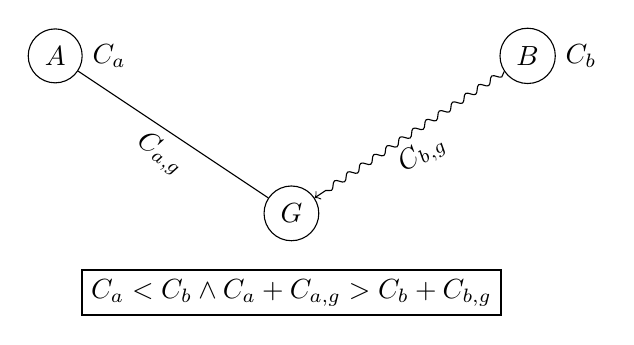
\begin{tikzpicture}[stateS/.style={shape=circle,draw=black},costC/.style={below,sloped,midway},costS/.style={anchor=west}]
\node[stateS] (A) at (-3,0) {$A$};
\node[costS] (cA) at (A.east) {$C_a$};
\node[stateS] (B) at (3,0) {$B$};
\node[costS] (cB) at (B.east) {$C_b$};
\node[stateS] (G) at (0,-2) {$G$};
\node[anchor=north,yshift=-10,shape=rectangle,draw=black,thick] (M) at (G.south) {$C_a<C_b\wedge C_a+C_{a,g}>C_b+C_{b,g}$};
\draw (A) to node[costC]{$C_{a,g}$} (G);
\draw[->,decorate,decoration={snake,amplitude=.4mm,segment length=2mm,post length=1mm}] (B) to node[costC]{$C_{b,g}$} (G);
\end{tikzpicture}
\caption{Algemeen geval van falen bij Uniform Cost Search}
\label{fig:badUniformCost}
\end{figure}
\begin{leftbar}
We passen bovendien dit algoritme toe op ons wegenplan, en bekomen een niet optimaal pad of figuur \ref{fig:uniformCostCity} op pagina \pageref{fig:uniformCostCity}, waar de kost 15 is, in plaats van 13.
\end{leftbar}
Dit algoritme geeft wel in de meeste gevallen al een behoorlijk optimale oplossing. Dit algoritme wordt beschreven in \algref{alg:uniformCost}.
\begin{algorithm}[htb]
\caption{Uniform Cost zoekalgoritme}
\label{alg:uniformCost}
\begin{algorithmic}[1]
\STATE $\queue\leftarrow\mbox{Path containing the root}$
\WHILE{$\notempty{\queue}\wedge\neg\goalreached{\queue}$}
\STATE $r\leftarrow\dequeue{\queue}$
\STATE $R\leftarrow\createnewpaths{r}$
\STATE $\removeloops{R}$
\STATE $\enqueue{\queue,R}$\COMMENT{De plaats doet er niet toe, de $\queue$ wordt nog gesorteerd}
\STATE $\quicksort{\queue,c}$
\ENDWHILE
\IF{$\goalreached{\queue}$}
\RETURN $\success$
\ELSE
\RETURN $\failure$
\ENDIF
\end{algorithmic}
\end{algorithm}
Indien we het loopdetectie-systeem even buiten beschouwing laten in onze tijds- en geheugencomplexiteitsanalyse, bekomen we volgende criteria:
\begin{center}
\begin{tabular}{ll}
\textbf{Compleet}:&Ja\\
\textbf{Snelheid}:&\bigoh{b^d}\\
\textbf{Geheugen}:&\bigoh{b^d}\\
\textbf{Optimaal}:&Nee
\end{tabular}
\end{center}
\subsubsection{Optimal Uniform Cost Algorithm}
Het \termen{Optimal Uniform Cost Algorithm}, garandeert wel een optimale oplossing, dit wordt gegarandeerd door het \termen{Branch-and-Bound Principe}. Dat principe zegt dat eenmaal we een pad dat naar een doel wijst gevonden hebben, we alle paden met een accumulatieve kost groter dan dat pad niet meer dienen te beschouwen (de kost neemt immers alleen maar toe). Indien onze $\queue$ een pad bevat dat naar een doel wijst, en dit komt als eerste voor, weten we zeker dat dit het optimale pad is. Gebasseerd op deze theorie herschrijven we dus onze terminatieconditie van het Uniform Cost Algorithm. Dit algoritme wordt beschreven in \algref{alg:optimalUniformCost}.
\begin{algorithm}[htb]
\caption{Optimal Uniform Cost zoekalgoritme}
\label{alg:optimalUniformCost}
\begin{algorithmic}[1]
\STATE $\queue\leftarrow\mbox{Path containing the root}$
\WHILE{$\notempty{\queue}\wedge\neg\goalreached{\queue\left[0\right]}$}
\STATE $r\leftarrow\dequeue{\queue}$
\STATE $R\leftarrow\createnewpaths{r}$
\STATE $\removeloops{R}$
\STATE $\enqueue{\queue,R}$\COMMENT{De plaats doet er niet toe, de $\queue$ wordt nog gesorteerd}
\STATE $\quicksort{\queue,c}$
\ENDWHILE
\IF{$\goalreached{\queue\left[0\right]}$}
\RETURN $\success$
\ELSE
\RETURN $\failure$
\ENDIF
\end{algorithmic}
\end{algorithm}
Indien we het loopdetectie-systeem even buiten beschouwing laten in onze tijds- en geheugencomplexiteitsanalyse, bekomen we volgende criteria:
\begin{center}
\begin{tabular}{ll}
\textbf{Compleet}:&Ja\\
\textbf{Snelheid}:&\bigoh{b^d}\\
\textbf{Geheugen}:&\bigoh{b^d}\\
\textbf{Optimaal}:&Ja
\end{tabular}
\end{center}
\begin{leftbar}
Een concrete uitwerking van dit algoritme wordt weergegeven op figuur \ref{fig:optimalUniformCostCity} op pagina \pageref{fig:optimalUniformCostCity}. We merken op dat deze gegarandeerde optimaliteit echter een grote hoeveelheid extra werk kan betekenen (66\% extra werk voor een oplossing die slechts 13\% beter is).
\end{leftbar}
\subsubsection{Extended Uniform Cost}
Het Optimal Uniform Cost algoritme werkt goed zolang de constraint $c\left(p_i,p_{i+1}\right)>0$ stand houdt, met andere woorden dat de kost tussen elke boog groter is dan 0. Het nadeel van dit zoekalgoritme is echter dat er opnieuw weinig probleem gerelateerde informatie aan te pas komt. Een oplossing bestaat erin een nieuwe functie te defini\"eren: de \termen{Extended Uniform Cost} $f:\Pp\rightarrow\Rr:p\mapsto r=f\left(p\right)$:
\begin{equation}
f\left(p\right)=c\left(p\right)+h\left(p_{\mbox{\small{end state}}}\right)
\end{equation}
Dit is dus de som van de reeds gemaakte kosten $c$, en een schatting $h$ van de nog te maken kosten tot de oplossing. Samen vormt dit dus een schatting van de kosten die we zullen betalen voor een pad naar het doel, met als subpad het huidige pad. Met deze functie kunnen we algoritmen ontwikkelen die gerichter op zoek gaan naar een oplossing, maar waarbij de optimaliteit behouden blijft.
\subsubsection{Estimate-extended Uniform Cost Algorithm}
Een algoritme die gebruik maakt van de Extended Uniform Cost is het \termen{Estimate-extended Uniform Cost Algorithm}. Dit is een variant op het Optimal Uniform Cost Algorithm, maar waarbij de knopen op de Extended Uniform Cost $f$ gesorteerd worden in plaats van de Uniform Cost $c$. Dit algoritme wordt beschreven in \algref{alg:estimateExtendedUniformCost}.
\begin{algorithm}[htb]
\caption{Estimate-extended Uniform Cost zoekalgoritme}
\label{alg:estimateExtendedUniformCost}
\begin{algorithmic}[1]
\STATE $\queue\leftarrow\mbox{Path containing the root}$
\WHILE{$\notempty{\queue}\wedge\neg\goalreached{\queue\left[0\right]}$}
\STATE $r\leftarrow\dequeue{\queue}$
\STATE $R\leftarrow\createnewpaths{r}$
\STATE $\removeloops{R}$
\STATE $\enqueue{\queue,R}$\COMMENT{De plaats doet er niet toe, de $\queue$ wordt nog gesorteerd}
\STATE $\quicksort{\queue,f}$
\ENDWHILE
\IF{$\goalreached{\queue\left[0\right]}$}
\RETURN $\success$
\ELSE
\RETURN $\failure$
\ENDIF
\end{algorithmic}
\end{algorithm}
Dit algoritme komt tot een optimale oplossing wanneer we echter nog een extra constraint plaatsen op de heuristiek. Als we het terminatiecriterium bekijken moet de meest optimale oplossing op het einde van het algoritme vooraan staan. Eventueel kunnen paden, die op dat moment echter een ongunstige heuristiek hebben, toch nog optimalere oplossingen opleveren. Het zou kunnen gebeuren dat optimale paden uit de boot vallen, indien op dat moment de heuristiek de nog te maken kosten overschat. De oplossing is het stellen dat de heuristiek altijd een \termen{Onderschatting} moet zijn van de nog te nemen kost tot een doel. Met andere woorden:
\begin{equation}
h\left(T\right)\leq c\left(T_{\mbox{\small{end point}}}\ldots\goal\right)
\end{equation}
Over het algemeen presteren deze algoritmen goed indien een goede heuristische functie gekozen wordt. Het berekenen van de functie impliceert echter ook overhead, bijgevolg is de beste heuristiek niet altijd geschikt om te zoeken. Indien we het loopdetectie-systeem even buiten beschouwing laten in onze tijds- en geheugencomplexiteitsanalyse, bekomen we volgende criteria:
\begin{center}
\begin{tabular}{ll}
\textbf{Compleet}:&Ja\\
\textbf{Snelheid}:&\bigoh{b^d}\\
\textbf{Geheugen}:&\bigoh{b^d}\\
\textbf{Optimaal}:&Ja (mits onderschatting)
\end{tabular}
\end{center}
\begin{leftbar}
Een uitgewerkt voorbeeld van Estimate-Extended Uniform Cost Search op het wegenplan wordt beschreven op figuur \ref{fig:estimateExtendedUniformCostCity} op pagina \pageref{fig:estimateExtendedUniformCostCity}.
\end{leftbar}
\subsubsection{Path Deletion}
Een andere uitbreiding die we kunnen toepassen en die algemeen toepasbaar is, is \termen{Path Deletion}. Bij het genereren van de boom genereren we vaak dezelfde toestand in verschillende takken van de boom (volgens het principe ``vele wegen leiden naar Rome''). We kunnen echter door de evaluatie van \'e\'en van deze staten tot een oplossing komen. Evaluatie van de andere versies leidt alleen maar tot overhead, en enkel de versie van de staat met de tot dan toe laagste cummulatieve kost komt in aanmerking voor een optimale oplossing. Path Deletion verwijdert de paden uit de queue die overhead veroorzaken. Indien er al een pad bestaat met dezelfde eindstaat, en de kost van dat pad is lager, is het niet nodig om de paden met eenzelfde eindpunt maar een hogere kost in de wachtrij te houden. Deze zullen immers altijd een hogere kost behouden. Of meer formeel in \algref{alg:pathDeletion}.
\begin{algorithm}[htb]
\caption{Path Deletion Principe}
\label{alg:pathDeletion}
\begin{algorithmic}[1]
\IF{$P\in\queue\wedge P=\left(\rootR,\ldots,I\right)\wedge Q\in\queue\wedge Q=\left(\rootR,\ldots,I,\ldots\right)\wedge c\left(P\right)\geq c\left(Q\right)$}
\STATE $\delete{\queue,P}$
\ENDIF
\end{algorithmic}
\end{algorithm}
\subsubsection{A* Search}
Het populairste zoekalgoritme bij uitstek is \termen{A* Search}, die eigenlijk een combinatie is van het beste uit verschillende zoekalgoritmen. A* is een uitbreiding op het Extended Uniform Cost Search Algoritme waarbij men het Branch-and-Bound principe, Heuristische Underestimate en de Redudant Path Deletion uitbreidingen toevoegt. Dit algoritme wordt beschreven in \algref{alg:aStar}. Een uitgewerkt voorbeeld staat op figuur \ref{fig:aStarCity} op pagina \pageref{fig:aStarCity}.
\begin{algorithm}[htb]
\caption{A* zoekalgoritme}
\label{alg:aStar}
\begin{algorithmic}[1]
\STATE $\queue\leftarrow\mbox{Path containing the root}$
\WHILE{$\notempty{\queue}\wedge\neg\goalreached{\queue\left[0\right]}$}
\STATE $r\leftarrow\dequeue{\queue}$
\STATE $R\leftarrow\createnewpaths{r}$
\STATE $\removeloops{R}$
\STATE $\enqueue{\queue,R}$\COMMENT{De plaats doet er niet toe, de $\queue$ wordt nog gesorteerd}
\STATE $\quicksort{\queue,f}$
\STATE\COMMENT{Path Deletion}
\FORALL{$P,Q\in\queue$}
\IF{$P=\left(\rootR,\ldots,I\right)\wedge Q=\left(\rootR,\ldots,I,\ldots\right)\wedge c\left(P\right)\geq c\left(Q\right)$}
\STATE $\delete{\queue,P}$
\ENDIF
\ENDFOR
\ENDWHILE
\IF{$\goalreached{\queue\left[0\right]}$}
\RETURN $\success$
\ELSE
\RETURN $\failure$
\ENDIF
\end{algorithmic}
\end{algorithm}
Vanwege de populariteit van A* zullen we wat dieper ingaan op enkele eigenschappen van A*.
\paragraph{Bewijs van Optimaliteit}
Alvorens we A* kunnen gebruiken, moeten we eerst een bewijs kunnen formuleren die borg staat dat A* altijd tot een optimale oplossing zal komen. Hiervoor maken we gebruik van enkele eigenschappen die we ook formeel aantonen. Hierbij stelt $B$ het meest optimale pad van de bron naar het doel voor.
\begin{theorem}
Voor ieder subpad $p$ van $B$ is de uitgebreide kost van $p$ kleiner of gelijk aan de kost van $B$. $\forall p \mbox{ subpath of } B: f\left(p\right)\leq c\left(B\right)$
\end{theorem}
\begin{proof}
\[
\begin{array}{c}
f\left(p\right)=c\left(p\right)+h\left(p_{\mbox{\small{end point}}}\right)\wedge h\left(p_{\mbox{\small{end point}}}\right)\leq c\left(p_{\mbox{\small{end point}}}\ldots\goal\right)\\
\Downarrow\\
f\left(p\right)\leq c\left(p\right)+c\left(p_{\mbox{\small{end point}}}\ldots\goal\right)=c\left(p,\ldots,\goal\right)=c\left(B\right)
\end{array}
\]
\end{proof}
\begin{theorem}
Tijdens iedere while test van A* bevat de $\queue$ een subpad van $B$
\label{the:astarsubpath}
\end{theorem}
\begin{proof}
\[
\begin{array}{c}
\mbox{bewijs door middel van inductie}:\\\\
\begin{array}{ll}
\mbox{\underline{Initieel:} }&S=\mbox{pad dat de bron bevat } \in\queue\wedge S \mbox{ is een subpad van } B\\
&\Downarrow\\
&\mbox{subpad van }B\in\queue\\\\
\mbox{\underline{Iteratie:} }&\mbox{indien een subpad van $B$ verwijdert wordt}\\\\
&\mbox{- het subpad heeft ten minste een kind (anders bestaat er geen $B$)}\\
&\mbox{- bovendien bevat dat kind geen lus ($B$ bevat geen lus)}\\\\
&\Rightarrow\mbox{Dit kind wordt weer toegevoegd aan de $\queue$}\\
&\Rightarrow\mbox{een subpad van }B\in\queue\\\\
\end{array}
\end{array}
\]
\end{proof}
\begin{corollary}
Voor ieder pad $p$ zodat $f\left(p\right)>c\left(B\right)$, kan $p$ nooit geselecteerd worden (Het zal nooit als eerste in de $\queue$ zitten).
\end{corollary}
\begin{proof}
\[
\begin{array}{c}
\begin{array}{rcl}
\mbox{altijd een subpad $q$ van}&\wedge&f\left(q\right)\leq c\left(B\right)<f\left(p\right)\\
\mbox{$B$ met } f\left(q\right)\leq c\left(B\right)&&\\
&\Downarrow&\\
\multicolumn{3}{c}{\mbox{$p$ wordt nooit geselecteerd}}
\end{array}
\end{array}
\]
\end{proof}
\paragraph{Bewijs van terminatie}
Stel $d$ is een natuurlijk getal $>c\left(B\right)/\delta$ (hierbij is $\delta$ de kleinste kost van alle bogen), en stel $P$ een pad van lengte $d$. In dat geval geldt:
\begin{equation}
f\left(P\right)=c\left(P\right)+h\left(P\right)\geq c\left(P\right)\geq d\cdot\delta>c\left(B\right)=f\left(B\right)
\end{equation}
We weten dus dat het pad $P$ nooit geselecteerd zal worden ($B$ is immers een pad dat het doel bereikt, en heeft een lagere $f$-waarde). Omdat we uitgaan van een eindige vertakkingsfactor $b$, zijn er dus maar een eindig aantal knopen die in de $\queue$ geplaatst kunnen worden. Omdat telkens wanneer we de lus uitvoeren er \'e\'en element uit de $\queue$ gehaald wordt, zal de $\queue$ op een gegeven moment leeg zijn, waardoor de lus doorbroken wordt en het algoritme stopt.
\paragraph{Bewijs van compleetheid}
Door theorema \ref{the:astarsubpath} kunnen we bewijzen dat het pad dat uiteindelijk zal evolueren naar een doel altijd in de $\queue$ zit, bijgevolg zal A* altijd het doel vinden.
\paragraph{Selectiegedrag van A*}
Welke knopen zullen ge\"expandeert worden? We kunnen de impliciete boom onderverdelen in drie verschillende groepen:
\begin{itemize}
 \item \termen{Nooit geselecteerde knopen}: Hierbij is $f\left(p\right)>c\left(B\right)$ of een redundant pad.
 \item \termen{Misschien geselecteerd knopen}: Hierbij is $f\left(p\right)=c\left(B\right)$
 \item \termen{Geselecteerde knopen}: Hierbij is $p\in\queue\wedge p\mbox{ is niet redundant}\wedge f\left(p\right)<c\left(B\right)$
\end{itemize}
\paragraph{Heuristische kracht}
\termen{Heuristical Power} gaat over in welke mate de heuristische functie belangrijk is voor het A* algoritme, en of we twee heuristische functies op de \'e\'en of andere manier kunnen vergelijken met elkaar. Door de constraint dat iedere heuristische functie alleen strikt positieve getallen moet teruggeven, en daarenboven een onderschatting moet zijn van de nog te nemen kost, kunnen we aantonen dat de heuristische functie het A* algoritme in ieder geval niet slechter kan doen presteren dan bijvoorbeeld het Optimal Uniform Cost algoritme. Indien we echter naar een vergelijking tussen twee heuristische functies streven, is het zo dat een functie die bij iedere toestand een grotere waarde retourneert dan zijn tegenhanger per definitie beter is. Met andere woorden:
\begin{equation}
 h_1 \mbox{ is beter dan } h_2\leftrightarrow\forall s\in\Ss:h_1\left(s\right)\geq h_2\left(s\right)
\end{equation}
Dit kunnen we beargumenteren omdat een heuristische functie per definitie een onderschatting moet zijn voor de werkelijke nog te betalen kost, en dus de heuristiek waarschijnlijk realistischer zal zijn. Verder kunnen we ook nog formeel aantonen dat indien $h_1$ beter is dan $h_2$ en er bestaat een pad van de bron naar het doel, dan zal A* met $h_2$ alle knopen evalueren die A* onder $h_1$ ge\"evalueerd zou hebben, met andere woorden A* zal zo goed als altijd langer werken met een slechtere heuristiek dan met een betere, volgens onze definitie van beter.
\subparagraph{Minimale kost paden en monotoniciteit}
Als we \algref{alg:pathDeletion} dichter bekijken zien we een asymmetrie in het algoritme, dit resulteert in het feit dat niet elke redundante knoop ontdekt wordt. Indien we bijvoorbeeld een pad beschouwen $\left(S,A,C,D\right)$ dat bij $C$ een geaccumuleerde kost heeft van $5$, en we expanderen een ander pad zodat er een kind-pad ontstaat $\left(S,B,C\right)$ met een geaccumuleerde kost van $4$ zal het eerste pad niet verwijdert worden (zie figuur \ref{fig:badMonotonicity}, hierbij gebeurt evaluatie als volgt: $S$, $A$, $C$, $D$ en $B$).
\begin{figure}[htb]
\centering
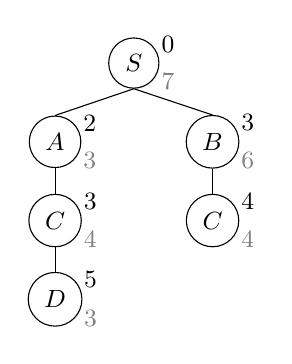
\begin{tikzpicture}[scale=0.5,stateS/.style={shape=circle,draw=black},costC/.style={below,sloped,midway},costS/.style={anchor=west},heurS/.style={gray,anchor=west}]
\node[stateS] (S) at (0,0) {\small $S$};
\node[costS] (cS) at (S.north east) {\small $0$};
\node[heurS] (hS) at (S.south east) {\small $7$};

\node[stateS] (A) at (-2,-2) {\small $A$};
\node[costS] (cA) at (A.north east) {\small $2$};
\node[heurS] (hA) at (A.south east) {\small $3$};

\node[stateS] (C) at (-2,-4) {\small $C$};
\node[costS] (cC) at (C.north east) {\small $3$};
\node[heurS] (hC) at (C.south east) {\small $4$};

\node[stateS] (D) at (-2,-6) {\small $D$};
\node[costS] (cD) at (D.north east) {\small $5$};
\node[heurS] (hD) at (D.south east) {\small $3$};

\node[stateS] (B) at (2,-2) {\small $B$};
\node[costS] (cB) at (B.north east) {\small $3$};
\node[heurS] (hB) at (B.south east) {\small $6$};

\node[stateS] (C2) at (2,-4) {\small $C$};
\node[costS] (cC2) at (C2.north east) {\small $4$};
\node[heurS] (hC2) at (C2.south east) {\small $4$};
\draw (S.south) -- (A.north);
\draw (A.south) -- (C.north);
\draw (C.south) -- (D.north);
\draw (S.south) -- (B.north);
\draw (B.south) -- (C2.north);
\end{tikzpicture}
\caption{Concreet geval van een niet monotone heuristiek}
\label{fig:badMonotonicity}
\end{figure}
Het is immers al het verst uitgebreid, en de kost is niet lager. Deze situatie kan voorkomen indien de heuristiek van $B$ bijvoorbeeld heel hoog was, terwijl deze van $A$ en $C$ veel kleiner waren. We kunnen het Path Deletion algoritme in principe niet al te veel aanpassen zodat het hier ook rekening mee houdt. Dit komt omdat deze knoop al ge\"expandeert is en we dus dubbel werk willen vermijden. Anderzijds kunnen we een constraint opleggen op onze heuristiek zodat deze nooit tot dergelijk situaties kan leiden. Deze constraint heet \termen{Monotoniciteit} of \termen{Monotonicity}. Deze stelt dat indien we een staat $A$ hebben, en $B$ is hiervan een kind, dan moet de heuristische waarde van $A$ kleiner of gelijk zijn aan de heuristische waarde van $B$ en de kost van $A$ naar $B$, of meer formeel:
\begin{equation}
B\mbox{ is een kind van }A\rightarrow h\left(A\right)\leq h\left(B\right)+c\left(A,B\right)
\end{equation}
Opnieuw is deze maatregel redelijk: indien immers niet aan de monotoniciteitsregel wordt voldaan betekent dit dat de heuristiek van $B$ een nog grotere onderschatting van het pad is dan de heuristiek van $A$. We weten na de heuristiek van $A$ te hebben ge\"evalueerd reeds dat we meer kosten zullen hebben dan die heuristiek. Indien $B$ een grotere onderschatting is, weten we eigenlijk helemaal niets nieuws. De heuristiek van $B$ zou in dat geval informatieloos zijn. A* zal indien we de monotoniciteitsregel volgen altijd een knoop selecteren met het meest effici\"entste pad tot de knoop. Verder kunnen we ook het Redudant Path algoritme optimaliseren onder deze voorwaarde, zoals in \algref{alg:optimalPathDeletion}.
\begin{algorithm}[htb]
\caption{Geoptimaliseerd Path Deletion Principe}
\label{alg:optimalPathDeletion}
\begin{algorithmic}[1]
\STATE ${\mathfrak H}\leftarrow\varnothing$
\IF{A* selecteerd een pad $p$}
\STATE $s\leftarrow p_{\mbox{end state}}$
\IF{$\hashtablecontains{{\mathfrak H},s}$}
\STATE do not evaluate $p$
\ELSE
\STATE $\inserthashtable{{\mathfrak H},s}$
\ENDIF
\ENDIF
\end{algorithmic}
\end{algorithm}
Hierdoor wordt path deletion vrijwel altijd gedaan in \bigoh{1}.
\paragraph{Pathmax}
\termen{Pathmax} is een variant van A* die deze monotoniciteitsregel afdwingt. Dit kan op verschillende manieren gedaan worden:
\begin{itemize}
 \item Corrigeren van de waarde van $f$: Indien $B$ een kind is van $A$ en $f\left(S,\ldots,A,B\right)<f\left(S,\ldots,A,\right)$ dan nemen we voor $f\left(S,\ldots,A,B\right)$ dezelfde waarde als $f\left(S,\ldots,A\right)$.
 \item $f$ herdefini\"eren: we genereren zelf een functie $f'$ die we defini\"eren als
\begin{equation}
f'\left(S,\ldots,A,B\right)=\mathfunc{max}{c\left(S,\ldots,A,B\right)+h\left(B\right),f'\left(S,\ldots,A\right)}
\end{equation}
\end{itemize}
\subsubsection{Iterative Deepening A* (IDA*)}
Een variant van A* is \termen{Iterative Deepening A*} of afgekort \termen{IDA*}. Deze heeft tot doel het geheugengebruik van A* meer onder controle te houden (we kunnen A* immers in de verte vergelijken met breedte-eerst, en dit algoritme is niet zuinig met geheugen). Net als Iterative Deepening een beperking op de diepte stelt voor Depth-First, stelt IDA* een beperking op de $f$ waarde. Indien we verwachten dat de oplossing bijvoorbeeld een $f$-waarde zal hebben van 100 zal het algoritme de kinderen van ge\"evalueerde knopen niet meer opslaan indien deze een $f$-waarde groter hebben dan 100. Uiteraard kan het gebeuren dat onze schatting niet toereikend was om tot een oplossing te komen, in dat geval wordt de $f$-waarde verhoogt en voeren \termen{$f$-limited Search} opnieuw uit. Meestal wordt als begin $f$-waarde de $f$-waarde van de bron $f\left(S\right)$ genomen, al dan niet vermenigvuldigt met een factor. Verder wordt de $f$-limiet meestal verhoogt naar de minimale $f$ die groter was dan de $f$-limiet. Dit wordt beschreven in \algref{alg:iterativeDeepeningAStar}.
\begin{algorithm}[htb]
\caption{Iterative Deepening A* zoekalgoritme}
\label{alg:iterativeDeepeningAStar}
\begin{algorithmic}[1]
\STATE $\fbound\leftarrow f\left(S\right)$\COMMENT{Or another $\fbound$-offset value}
\STATE $\queue\leftarrow\varnothing$
\WHILE{$\neg\goalreached{\queue}$}
\STATE\COMMENT{Begin $f$-limited Search}
\STATE $\queue\leftarrow\mbox{Path containing the root}$
\STATE $\fnew\leftarrow\infty$
\WHILE{$\notempty{\queue}$}
\STATE $r\leftarrow\dequeue{\queue}$
\STATE $R\leftarrow\createnewpaths{r}$
\STATE $\removeloops{R}$
\STATE $\fnew\leftarrow\minM{}{\fnew,f\left(\minM{f}{\select{R,\left(R_i\right)>\fbound}}\right)}$
\STATE $\removeif{R,f\left(R_i\right)>\fbound}$
\STATE\COMMENT{Because we will evaluate them all the nodes lower than}
\STATE\COMMENT{a certain $f$-value we don't have to sort them in any order}
\STATE $\enqueuefront{\queue,R}$
\STATE\COMMENT{Path Deletion}
\IF{$P,Q\in\queue\wedge P=\left(\rootR,\ldots,I\right)\wedge Q=\left(\rootR,\ldots,I,\ldots\right)\wedge c\left(P\right)\geq c\left(Q\right)$}
\STATE $\delete{\queue,P}$
\ENDIF
\ENDWHILE
\STATE\COMMENT{Einde $f$-limited Search}
\STATE $\fbound\leftarrow\fnew$
\ENDWHILE
\end{algorithmic}
\end{algorithm}
Indien we het loopdetectie- en path deletion-systeem even buiten beschouwing laten in onze tijds- en geheugencomplexiteitsanalyse, bekomen we volgende criteria:
\begin{center}
\begin{tabular}{ll}
\textbf{Compleet}:&Ja\\
\textbf{Snelheid}:&\bigoh{N^2}\\
\textbf{Geheugen}:&\bigoh{b\cdot c\left(B\right)/\delta}\\
\textbf{Optimaal}:&Ja\\
\end{tabular}
\end{center}
\subsubsection{Simplified Memory-bounded A* (SMA*)}
Een gelijkaardig effect probeert \termen{Simplified Memory-bounded A*} (of kortweg \termen{SMA*}) te bereiken. Hierbij is het geheugen echter begrensd, en moeten we proberen om in deze beperkende omstandigheden toch een optimale oplossing te vinden. Dit behoorlijke complexe algoritme heeft als basisidee dat indien het geheugen vol is, en we moeten een knoop evalueren, de knopen met de hoogste $f$-waarde tijdelijk uit het geheugen worden gelaten. Om echter geen overbodig werkt te doen in het herberekenen van alle knopen veranderen we de $f$-waarde van de ouder. De ouder van een te verwijderen knoop houdt telkens de beste (laagste) $f$-waarde van van zijn kinderen bij. Deze $f$-waardes spelen vervolgens nog een rol om de knopen opnieuw te evalueren, en te zoeken naar een eventueel doel.
\paragraph{}Een belangrijk aspect hierbij is dat kinderen \'e\'en voor \'e\'en gegenereerd worden om geen \termen{Memory Overflow} te bekomen. Indien het geheugen vol is, moet een knoop wijken voor de te genereren knoop. Verder kan dit algoritme uiteraard geen doelen vinden waarbij het pad naar het doel meer geheugen vereist dan er beschikbaar is. Het algoritme is echter wel compleet wanneer er voldoende geheugen voorradig is.
\subsection{Besluitende commentaren}
\subsubsection{Niet Optimale Varianten}
Tot dusver zochten we altijd naar optimale oplossingen, soms is het echter beter om niet de meest optimale oplossing te zoeken indien dit tijdswinst kan opleveren. Indien we gebruik maken van \termen{Non-optimal variants}, is dit meestal door de heuristiek aan te passen. Deze zullen meestal het onderschattings-aspect achterwege laten, en worden meestal \termen{Non-admissible heuristics} genoemd. Een andere mogelijkheid is het toepassen van een ander zoekalgoritme. Een variant van A*, het \termen{Non-admissible A* Search Algorithm} is hier een voorbeeld van. Hierbij wordt $f$ als volgt gedefinieerd:
\begin{equation}
f\left(p\right)=\left.\omega\cdot c\left(p\right)+h\left(p_{\mbox{\small{end state}}}\right)\ \ \ \ \right|\omega\in\left[0,1\right]
\end{equation}
Met $\omega$ als een parameter. Indien $\omega=1$ verkrijgen we opnieuw het A* algoritme, indien we $\omega=0$ nemen bekomen we opnieuw Greedy Search.
\subsubsection{Complexiteit in het algemeen}
Bij nature is het vinden van een optimaal pad dat naar een oplossing voor een dergelijke probleem NP-compleet. Er bestaan echter wel parallelle\footnote{Algoritmen die we kunnen uitvoeren op bijvoorbeeld vector-, DNA- en kwantumcomputers met massaparallellisme.} algoritmen die in polynomiale tijd kunnen werken.
\paragraph{}Meestal leidt dit tot een trade-off waarbij we de optimaliteit reduceren tot een behoorlijke optimale oplossing en hierbij een grote hoeveelheid tijd besparen naar het zoeken van de oplossing. Een voorbeeld hierbij is het instellen van $\omega$ bij Non-admissible A*: hoe meer $\omega$ naar $1$ gaat, hoe meer we in de buurt van een optimale oplossing komen.
\subsection{Samenvatting}
\label{app:SearchMethods}
\begin{table}[H]
\centering
\begin{tabular}{l|llll|l}
\hline
\textbf{Name}&\textbf{Compleet}&\textbf{Optimaal}&\textbf{Snelheid}&\textbf{Geheugen}&\textbf{Alg.(p.)}\\\hline
\hline
\multicolumn{6}{l}{\textbf{Blind Search}}\\\hline
- Depth First&Ja&Nee&\bigoh{b^d}&\bigoh{b\cdot d}&\ref{alg:depthFirst}(\pageref{alg:depthFirst})\\\hline
- Breadth First&Ja&Nee&\bigoh{b^m}&\bigoh{b^m}&\ref{alg:breadthFirst}(\pageref{alg:breadthFirst})\\\hline
- Neen-Deterministic&Ja&Nee&\bigoh{b^d}&\bigoh{b^d}&\ref{alg:nonDeterministic}(\pageref{alg:nonDeterministic})\\\hline
- Iterative Deepening&Ja&Nee&\bigoh{b^m}&\bigoh{b\cdot m}&\ref{alg:iterativeDeepening}(\pageref{alg:iterativeDeepening})\\\hline
- Bi-Direction Search&Ja&Nee&\bigoh{b^{m/2}}&\bigoh{b^{m/2}}&\ref{alg:biDirectional}(\pageref{alg:biDirectional})\\\hline
\multicolumn{6}{l}{\textbf{Heuristic Search}}\\\hline
- Hill Climbing&Ja&Nee&\bigoh{b^d}&\bigoh{b\cdot d}&\ref{alg:hillClimbing}(\pageref{alg:hillClimbing})\\\hline
- Beam Search&Nee&Nee&\bigoh{w\cdot m}&\bigoh{w}&\ref{alg:beamSearch}(\pageref{alg:beamSearch})\\\hline
- Hill Climbing 2&Nee&Nee&\bigoh{m}&\bigoh{b}&\ref{alg:hillClimbing2}(\pageref{alg:hillClimbing2})\\\hline
- Greedy Search&Ja&Nee&\bigoh{b^d}&\bigoh{b^d}&\ref{alg:greedy}(\pageref{alg:greedy})\\\hline
\multicolumn{6}{l}{\textbf{Optimal Search}}\\\hline
- Uniform Cost&Ja&Nee&\bigoh{b^d}&\bigoh{b^d}&\ref{alg:uniformCost}(\pageref{alg:uniformCost})\\\hline
- Optimal Uniform Cost&Ja&Ja&\bigoh{b^d}&\bigoh{b^d}&\ref{alg:optimalUniformCost}(\pageref{alg:optimalUniformCost})\\\hline
- Estimate-extended Uniform Cost&Ja&Ja&\bigoh{b^d}&\bigoh{b^d}&\ref{alg:estimateExtendedUniformCost}(\pageref{alg:estimateExtendedUniformCost})\\\hline
- A*&Ja&Ja&\bigoh{b^d}&\bigoh{b^d}&\ref{alg:aStar}(\pageref{alg:aStar})\\\hline
- Iterative Deepening A*&Ja&Ja&\bigoh{N^2}&\bigoh{b\cdot c\left(B\right)/\delta}&\ref{alg:iterativeDeepeningAStar}(\pageref{alg:iterativeDeepeningAStar})\\\hline
- Simplified Memory-bounded A*&Ja&Ja&\bigoh{b^d}&\bigoh{1}&\\\hline
\end{tabular}
\caption{Samenvatting van de zoekmethodes}
\end{table}
Een samenvattend schema is te vinden in appendix \ref{app:schemaSearch} op pagina \pageref{app:schemaSearch}.
\newpage
\subsection{Toepassingen van de zoekalgoritmen (Afbeeldingen)}
\label{ss:cityFigures}
\subsubsection{Blind Search Methods}
\begin{figure}[H]
\centering
\subfigure{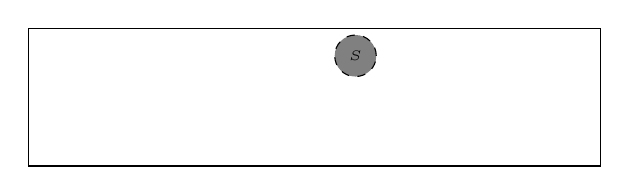
\begin{tikzpicture}[xscale=0.7,yscale=1.4,city/.style={shape=circle,draw=black},costc/.style={anchor=south east},heurh/.style={anchor=north east,gray},cityG/.style={city,very thick},cityM/.style={city,fill=gray}]
\def\dy{-0.75};
\def\dxa{4.75};
\def\dxb{2.875};
\def\dxc{1.125};
\def\dxd{0.75};
\def\dxe{0.75};

\draw (-0.5*\dxa-0.5*\dxb-\dxc-1,0.25) rectangle (0.5*\dxa+0.5*\dxb+\dxc-0.5,1*\dy-0.25);

\node[cityM,dashed] (S) at (0,0) {\tiny $S$};

\end{tikzpicture}}
\subfigure{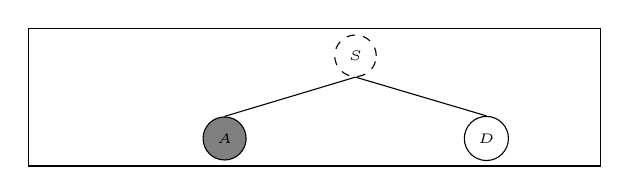
\begin{tikzpicture}[xscale=0.7,yscale=1.4,city/.style={shape=circle,draw=black},costc/.style={anchor=south east},heurh/.style={anchor=north east,gray},cityG/.style={city,very thick},cityM/.style={city,fill=gray}]
\def\dy{-0.75};
\def\dxa{4.75};
\def\dxb{2.875};
\def\dxc{1.125};
\def\dxd{0.75};
\def\dxe{0.75};

\draw (-0.5*\dxa-0.5*\dxb-\dxc-1,0.25) rectangle (0.5*\dxa+0.5*\dxb+\dxc-0.5,1*\dy-0.25);

\node[city,dashed] (S) at (0,0) {\tiny $S$};

\node[cityM] (A) at (-0.5*\dxa,\dy) {\tiny $A$};
\draw (S.south) -- (A.north);
\node[city] (D) at (0.5*\dxa,\dy) {\tiny $D$};
\draw (S.south) -- (D.north);

\end{tikzpicture}}
\subfigure{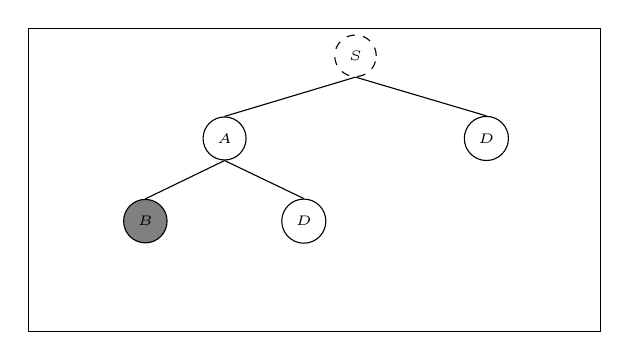
\begin{tikzpicture}[xscale=0.7,yscale=1.4,city/.style={shape=circle,draw=black},costc/.style={anchor=south east},heurh/.style={anchor=north east,gray},cityG/.style={city,very thick},cityM/.style={city,fill=gray}]
\def\dy{-0.75};
\def\dxa{4.75};
\def\dxb{2.875};
\def\dxc{1.125};
\def\dxd{0.75};
\def\dxe{0.75};

\draw (-0.5*\dxa-0.5*\dxb-\dxc-1,0.25) rectangle (0.5*\dxa+0.5*\dxb+\dxc-0.5,3*\dy-0.25);

\node[city,dashed] (S) at (0,0) {\tiny $S$};

\node[city] (A) at (-0.5*\dxa,\dy) {\tiny $A$};
\draw (S.south) -- (A.north);
\node[city] (D) at (0.5*\dxa,\dy) {\tiny $D$};
\draw (S.south) -- (D.north);

\node[cityM] (B) at (-0.5*\dxa-0.5*\dxb,2*\dy) {\tiny $B$};
\draw (A.south) -- (B.north);
\node[city] (D2) at (-0.5*\dxa+0.5*\dxb,2*\dy) {\tiny $D$};
\draw (A.south) -- (D2.north);
\end{tikzpicture}}
\subfigure{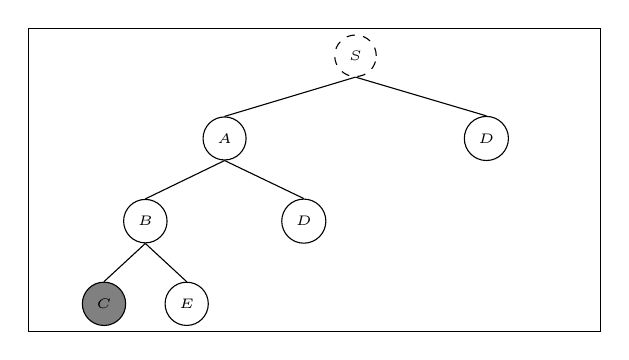
\begin{tikzpicture}[xscale=0.7,yscale=1.4,city/.style={shape=circle,draw=black},costc/.style={anchor=south east},heurh/.style={anchor=north east,gray},cityG/.style={city,very thick},cityM/.style={city,fill=gray}]
\def\dy{-0.75};
\def\dxa{4.75};
\def\dxb{2.875};
\def\dxc{1.125};
\def\dxd{0.75};
\def\dxe{0.75};

\draw (-0.5*\dxa-0.5*\dxb-\dxc-1,0.25) rectangle (0.5*\dxa+0.5*\dxb+\dxc-0.5,3*\dy-0.25);
\def\dxc{1.5};

\node[city,dashed] (S) at (0,0) {\tiny $S$};

\node[city] (A) at (-0.5*\dxa,\dy) {\tiny $A$};
\draw (S.south) -- (A.north);
\node[city] (D) at (0.5*\dxa,\dy) {\tiny $D$};
\draw (S.south) -- (D.north);

\node[city] (B) at (-0.5*\dxa-0.5*\dxb,2*\dy) {\tiny $B$};
\draw (A.south) -- (B.north);
\node[city] (D2) at (-0.5*\dxa+0.5*\dxb,2*\dy) {\tiny $D$};
\draw (A.south) -- (D2.north);

\node[cityM] (C) at (-0.5*\dxa-0.5*\dxb-0.5*\dxc,3*\dy) {\tiny $C$};
\draw (B.south) -- (C.north);
\node[city] (E2) at (-0.5*\dxa-0.5*\dxb+0.5*\dxc,3*\dy) {\tiny $E$};
\draw (B.south) -- (E2.north);
\end{tikzpicture}}
\subfigure{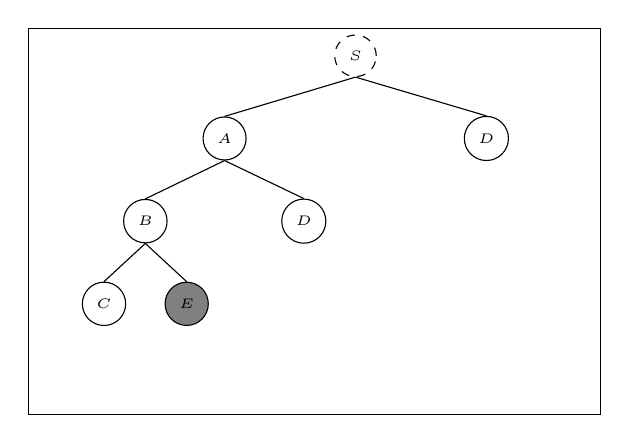
\begin{tikzpicture}[xscale=0.7,yscale=1.4,city/.style={shape=circle,draw=black},costc/.style={anchor=south east},heurh/.style={anchor=north east,gray},cityG/.style={city,very thick},cityM/.style={city,fill=gray}]
\def\dy{-0.75};
\def\dxa{4.75};
\def\dxb{2.875};
\def\dxc{1.125};
\def\dxd{0.75};
\def\dxe{0.75};

\draw (-0.5*\dxa-0.5*\dxb-\dxc-1,0.25) rectangle (0.5*\dxa+0.5*\dxb+\dxc-0.5,4*\dy-0.25);
\def\dxc{1.5};

\node[city,dashed] (S) at (0,0) {\tiny $S$};

\node[city] (A) at (-0.5*\dxa,\dy) {\tiny $A$};
\draw (S.south) -- (A.north);
\node[city] (D) at (0.5*\dxa,\dy) {\tiny $D$};
\draw (S.south) -- (D.north);

\node[city] (B) at (-0.5*\dxa-0.5*\dxb,2*\dy) {\tiny $B$};
\draw (A.south) -- (B.north);
\node[city] (D2) at (-0.5*\dxa+0.5*\dxb,2*\dy) {\tiny $D$};
\draw (A.south) -- (D2.north);

\node[city] (C) at (-0.5*\dxa-0.5*\dxb-0.5*\dxc,3*\dy) {\tiny $C$};
\draw (B.south) -- (C.north);
\node[cityM] (E2) at (-0.5*\dxa-0.5*\dxb+0.5*\dxc,3*\dy) {\tiny $E$};
\draw (B.south) -- (E2.north);
\end{tikzpicture}}
\subfigure{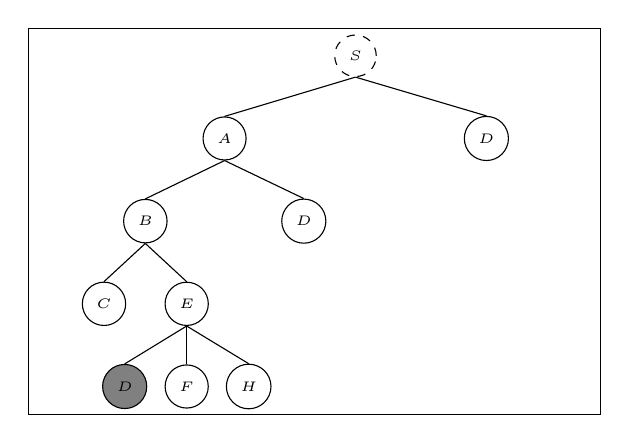
\begin{tikzpicture}[xscale=0.7,yscale=1.4,city/.style={shape=circle,draw=black},costc/.style={anchor=south east},heurh/.style={anchor=north east,gray},cityG/.style={city,very thick},cityM/.style={city,fill=gray}]
\def\dy{-0.75};
\def\dxa{4.75};
\def\dxb{2.875};
\def\dxc{1.125};
\def\dxd{1.125};
\def\dxe{0.75};

\draw (-0.5*\dxa-0.5*\dxb-\dxc-1,0.25) rectangle (0.5*\dxa+0.5*\dxb+\dxc-0.5,4*\dy-0.25);
\def\dxc{1.5};

\node[city,dashed] (S) at (0,0) {\tiny $S$};

\node[city] (A) at (-0.5*\dxa,\dy) {\tiny $A$};
\draw (S.south) -- (A.north);
\node[city] (D) at (0.5*\dxa,\dy) {\tiny $D$};
\draw (S.south) -- (D.north);

\node[city] (B) at (-0.5*\dxa-0.5*\dxb,2*\dy) {\tiny $B$};
\draw (A.south) -- (B.north);
\node[city] (D2) at (-0.5*\dxa+0.5*\dxb,2*\dy) {\tiny $D$};
\draw (A.south) -- (D2.north);

\node[city] (C) at (-0.5*\dxa-0.5*\dxb-0.5*\dxc,3*\dy) {\tiny $C$};
\draw (B.south) -- (C.north);
\node[city] (E2) at (-0.5*\dxa-0.5*\dxb+0.5*\dxc,3*\dy) {\tiny $E$};
\draw (B.south) -- (E2.north);

\node[cityM] (D3) at (-0.5*\dxa-0.5*\dxb+0.5*\dxc-\dxd,4*\dy) {\tiny $D$};
\draw (E2.south) -- (D3.north);
\node[city] (F2) at (-0.5*\dxa-0.5*\dxb+0.5*\dxc,4*\dy) {\tiny $F$};
\draw (E2.south) -- (F2.north);
\node[city] (H2) at (-0.5*\dxa-0.5*\dxb+0.5*\dxc+\dxd,4*\dy) {\tiny $H$};
\draw (E2.south) -- (H2.north);
\end{tikzpicture}}
\subfigure{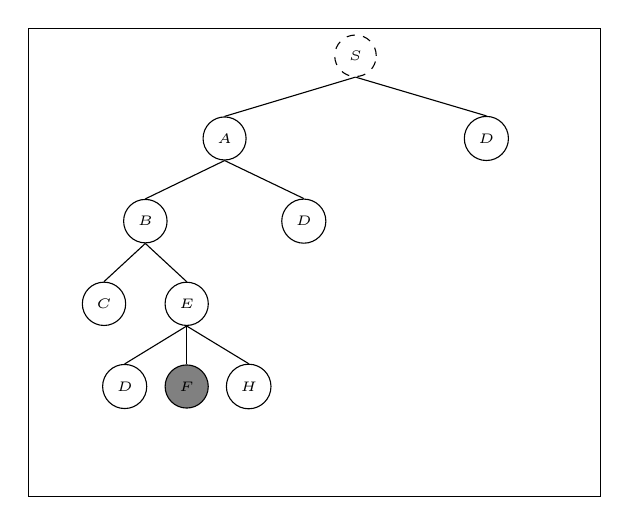
\begin{tikzpicture}[xscale=0.7,yscale=1.4,city/.style={shape=circle,draw=black},costc/.style={anchor=south east},heurh/.style={anchor=north east,gray},cityG/.style={city,very thick},cityM/.style={city,fill=gray}]
\def\dy{-0.75};
\def\dxa{4.75};
\def\dxb{2.875};
\def\dxc{1.125};
\def\dxd{1.125};
\def\dxe{0.75};

\draw (-0.5*\dxa-0.5*\dxb-\dxc-1,0.25) rectangle (0.5*\dxa+0.5*\dxb+\dxc-0.5,5*\dy-0.25);
\def\dxc{1.5};

\node[city,dashed] (S) at (0,0) {\tiny $S$};

\node[city] (A) at (-0.5*\dxa,\dy) {\tiny $A$};
\draw (S.south) -- (A.north);
\node[city] (D) at (0.5*\dxa,\dy) {\tiny $D$};
\draw (S.south) -- (D.north);

\node[city] (B) at (-0.5*\dxa-0.5*\dxb,2*\dy) {\tiny $B$};
\draw (A.south) -- (B.north);
\node[city] (D2) at (-0.5*\dxa+0.5*\dxb,2*\dy) {\tiny $D$};
\draw (A.south) -- (D2.north);

\node[city] (C) at (-0.5*\dxa-0.5*\dxb-0.5*\dxc,3*\dy) {\tiny $C$};
\draw (B.south) -- (C.north);
\node[city] (E2) at (-0.5*\dxa-0.5*\dxb+0.5*\dxc,3*\dy) {\tiny $E$};
\draw (B.south) -- (E2.north);

\node[city] (D3) at (-0.5*\dxa-0.5*\dxb+0.5*\dxc-\dxd,4*\dy) {\tiny $D$};
\draw (E2.south) -- (D3.north);
\node[cityM] (F2) at (-0.5*\dxa-0.5*\dxb+0.5*\dxc,4*\dy) {\tiny $F$};
\draw (E2.south) -- (F2.north);
\node[city] (H2) at (-0.5*\dxa-0.5*\dxb+0.5*\dxc+\dxd,4*\dy) {\tiny $H$};
\draw (E2.south) -- (H2.north);
\end{tikzpicture}}
\subfigure{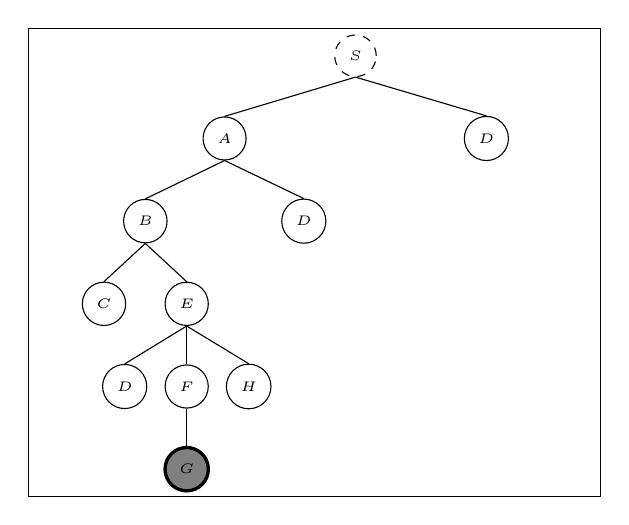
\begin{tikzpicture}[xscale=0.7,yscale=1.4,city/.style={shape=circle,draw=black},costc/.style={anchor=south east},heurh/.style={anchor=north east,gray},cityG/.style={city,very thick},cityM/.style={city,fill=gray},cityMG/.style={cityM,very thick},cityM/.style={city,fill=gray}]
\def\dy{-0.75};
\def\dxa{4.75};
\def\dxb{2.875};
\def\dxc{1.125};
\def\dxd{1.125};
\def\dxe{0.75};

\draw (-0.5*\dxa-0.5*\dxb-\dxc-1,0.25) rectangle (0.5*\dxa+0.5*\dxb+\dxc-0.5,5*\dy-0.25);
\def\dxc{1.5};

\node[city,dashed] (S) at (0,0) {\tiny $S$};

\node[city] (A) at (-0.5*\dxa,\dy) {\tiny $A$};
\draw (S.south) -- (A.north);
\node[city] (D) at (0.5*\dxa,\dy) {\tiny $D$};
\draw (S.south) -- (D.north);

\node[city] (B) at (-0.5*\dxa-0.5*\dxb,2*\dy) {\tiny $B$};
\draw (A.south) -- (B.north);
\node[city] (D2) at (-0.5*\dxa+0.5*\dxb,2*\dy) {\tiny $D$};
\draw (A.south) -- (D2.north);

\node[city] (C) at (-0.5*\dxa-0.5*\dxb-0.5*\dxc,3*\dy) {\tiny $C$};
\draw (B.south) -- (C.north);
\node[city] (E2) at (-0.5*\dxa-0.5*\dxb+0.5*\dxc,3*\dy) {\tiny $E$};
\draw (B.south) -- (E2.north);

\node[city] (D3) at (-0.5*\dxa-0.5*\dxb+0.5*\dxc-\dxd,4*\dy) {\tiny $D$};
\draw (E2.south) -- (D3.north);
\node[city] (F2) at (-0.5*\dxa-0.5*\dxb+0.5*\dxc,4*\dy) {\tiny $F$};
\draw (E2.south) -- (F2.north);
\node[city] (H2) at (-0.5*\dxa-0.5*\dxb+0.5*\dxc+\dxd,4*\dy) {\tiny $H$};
\draw (E2.south) -- (H2.north);

\node[cityMG] (G3) at (-0.5*\dxa-0.5*\dxb+0.5*\dxc,5*\dy) {\tiny $G$};
\draw (F2.south) -- (G3.north);
\end{tikzpicture}}
\caption{Depth-First toegepast op het wegenplan}
\label{fig:depthFirstCity}
\end{figure}
\begin{figure}[H]
\centering
\subfigure{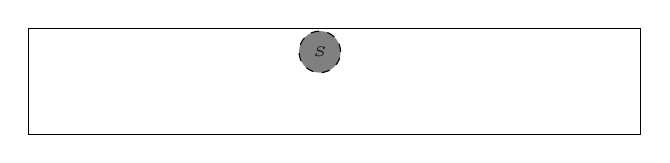
\begin{tikzpicture}[xscale=0.75,yscale=1,city/.style={shape=circle,draw=black},costc/.style={anchor=south east},heurh/.style={anchor=north east,gray},cityG/.style={city,very thick},cityM/.style={city,fill=gray}]
\def\dy{-0.75};
\def\dxa{4.75};
\def\dxb{2.875};
\def\dxc{1.125};
\def\dxd{0.75};
\def\dxe{0.75};

\draw (-0.5*\dxa-0.5*\dxb-\dxc,0.3) rectangle (0.5*\dxa+0.5*\dxb+\dxc+0.5,1*\dy-0.3);

\node[cityM,dashed] (S) at (0,0) {\tiny $S$};
\end{tikzpicture}}
\subfigure{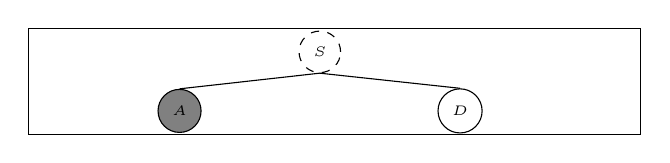
\begin{tikzpicture}[xscale=0.75,yscale=1,city/.style={shape=circle,draw=black},costc/.style={anchor=south east},heurh/.style={anchor=north east,gray},cityG/.style={city,very thick},cityM/.style={city,fill=gray}]
\def\dy{-0.75};
\def\dxa{4.75};
\def\dxb{2.875};
\def\dxc{1.125};
\def\dxd{0.75};
\def\dxe{0.75};

\draw (-0.5*\dxa-0.5*\dxb-\dxc,0.3) rectangle (0.5*\dxa+0.5*\dxb+\dxc+0.5,1*\dy-0.3);

\node[city,dashed] (S) at (0,0) {\tiny $S$};

\node[cityM] (A) at (-0.5*\dxa,\dy) {\tiny $A$};
\draw (S.south) -- (A.north);
\node[city] (D) at (0.5*\dxa,\dy) {\tiny $D$};
\draw (S.south) -- (D.north);
\end{tikzpicture}}
\subfigure{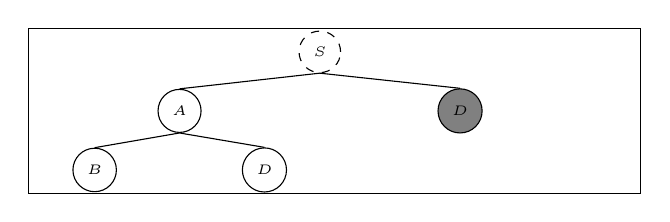
\begin{tikzpicture}[xscale=0.75,yscale=1,city/.style={shape=circle,draw=black},costc/.style={anchor=south east},heurh/.style={anchor=north east,gray},cityG/.style={city,very thick},cityM/.style={city,fill=gray}]
\def\dy{-0.75};
\def\dxa{4.75};
\def\dxb{2.875};
\def\dxc{1.125};
\def\dxd{0.75};
\def\dxe{0.75};

\draw (-0.5*\dxa-0.5*\dxb-\dxc,0.3) rectangle (0.5*\dxa+0.5*\dxb+\dxc+0.5,2*\dy-0.3);

\node[city,dashed] (S) at (0,0) {\tiny $S$};

\node[city] (A) at (-0.5*\dxa,\dy) {\tiny $A$};
\draw (S.south) -- (A.north);
\node[cityM] (D) at (0.5*\dxa,\dy) {\tiny $D$};
\draw (S.south) -- (D.north);

\node[city] (B) at (-0.5*\dxa-0.5*\dxb,2*\dy) {\tiny $B$};
\draw (A.south) -- (B.north);
\node[city] (D2) at (-0.5*\dxa+0.5*\dxb,2*\dy) {\tiny $D$};
\draw (A.south) -- (D2.north);
\end{tikzpicture}}
\subfigure{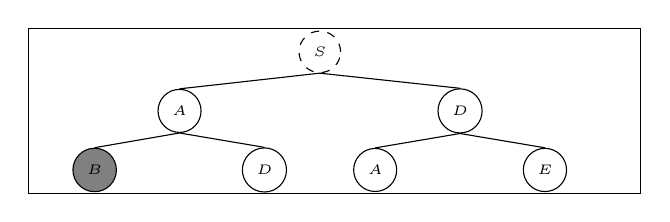
\begin{tikzpicture}[xscale=0.75,yscale=1,city/.style={shape=circle,draw=black},costc/.style={anchor=south east},heurh/.style={anchor=north east,gray},cityG/.style={city,very thick},cityM/.style={city,fill=gray}]
\def\dy{-0.75};
\def\dxa{4.75};
\def\dxb{2.875};
\def\dxc{1.125};
\def\dxd{0.75};
\def\dxe{0.75};

\draw (-0.5*\dxa-0.5*\dxb-\dxc,0.3) rectangle (0.5*\dxa+0.5*\dxb+\dxc+0.5,2*\dy-0.3);

\node[city,dashed] (S) at (0,0) {\tiny $S$};

\node[city] (A) at (-0.5*\dxa,\dy) {\tiny $A$};
\draw (S.south) -- (A.north);
\node[city] (D) at (0.5*\dxa,\dy) {\tiny $D$};
\draw (S.south) -- (D.north);

\node[cityM] (B) at (-0.5*\dxa-0.5*\dxb,2*\dy) {\tiny $B$};
\draw (A.south) -- (B.north);
\node[city] (D2) at (-0.5*\dxa+0.5*\dxb,2*\dy) {\tiny $D$};
\draw (A.south) -- (D2.north);
\node[city] (A2) at (0.5*\dxa-0.5*\dxb,2*\dy) {\tiny $A$};
\draw (D.south) -- (A2.north);
\node[city] (E) at (0.5*\dxa+0.5*\dxb,2*\dy) {\tiny $E$};
\draw (D.south) -- (E.north);
\end{tikzpicture}}
\subfigure{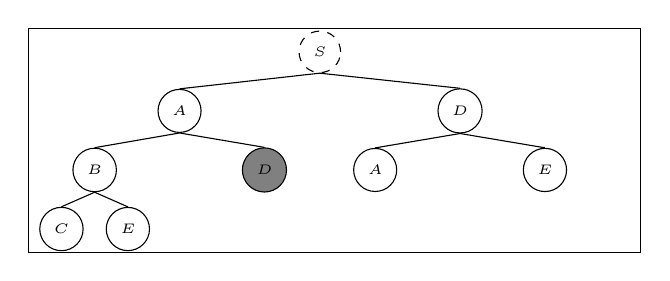
\begin{tikzpicture}[xscale=0.75,yscale=1,city/.style={shape=circle,draw=black},costc/.style={anchor=south east},heurh/.style={anchor=north east,gray},cityG/.style={city,very thick},cityM/.style={city,fill=gray}]
\def\dy{-0.75};
\def\dxa{4.75};
\def\dxb{2.875};
\def\dxc{1.125};
\def\dxd{0.75};
\def\dxe{0.75};

\draw (-0.5*\dxa-0.5*\dxb-\dxc,0.3) rectangle (0.5*\dxa+0.5*\dxb+\dxc+0.5,3*\dy-0.3);

\node[city,dashed] (S) at (0,0) {\tiny $S$};

\node[city] (A) at (-0.5*\dxa,\dy) {\tiny $A$};
\draw (S.south) -- (A.north);
\node[city] (D) at (0.5*\dxa,\dy) {\tiny $D$};
\draw (S.south) -- (D.north);

\node[city] (B) at (-0.5*\dxa-0.5*\dxb,2*\dy) {\tiny $B$};
\draw (A.south) -- (B.north);
\node[cityM] (D2) at (-0.5*\dxa+0.5*\dxb,2*\dy) {\tiny $D$};
\draw (A.south) -- (D2.north);
\node[city] (A2) at (0.5*\dxa-0.5*\dxb,2*\dy) {\tiny $A$};
\draw (D.south) -- (A2.north);
\node[city] (E) at (0.5*\dxa+0.5*\dxb,2*\dy) {\tiny $E$};
\draw (D.south) -- (E.north);

\node[city] (C) at (-0.5*\dxa-0.5*\dxb-0.5*\dxc,3*\dy) {\tiny $C$};
\draw (B.south) -- (C.north);
\node[city] (E2) at (-0.5*\dxa-0.5*\dxb+0.5*\dxc,3*\dy) {\tiny $E$};
\draw (B.south) -- (E2.north);
\end{tikzpicture}}
\subfigure{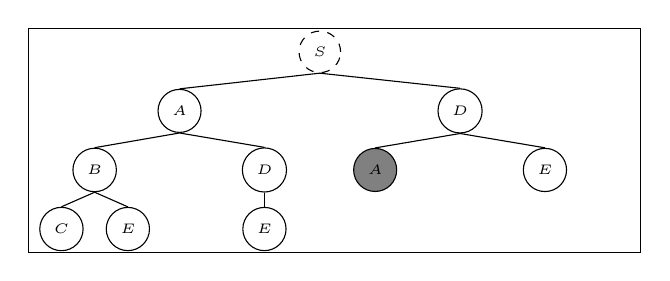
\begin{tikzpicture}[xscale=0.75,yscale=1,city/.style={shape=circle,draw=black},costc/.style={anchor=south east},heurh/.style={anchor=north east,gray},cityG/.style={city,very thick},cityM/.style={city,fill=gray}]
\def\dy{-0.75};
\def\dxa{4.75};
\def\dxb{2.875};
\def\dxc{1.125};
\def\dxd{0.75};
\def\dxe{0.75};

\draw (-0.5*\dxa-0.5*\dxb-\dxc,0.3) rectangle (0.5*\dxa+0.5*\dxb+\dxc+0.5,3*\dy-0.3);

\node[city,dashed] (S) at (0,0) {\tiny $S$};

\node[city] (A) at (-0.5*\dxa,\dy) {\tiny $A$};
\draw (S.south) -- (A.north);
\node[city] (D) at (0.5*\dxa,\dy) {\tiny $D$};
\draw (S.south) -- (D.north);

\node[city] (B) at (-0.5*\dxa-0.5*\dxb,2*\dy) {\tiny $B$};
\draw (A.south) -- (B.north);
\node[city] (D2) at (-0.5*\dxa+0.5*\dxb,2*\dy) {\tiny $D$};
\draw (A.south) -- (D2.north);
\node[cityM] (A2) at (0.5*\dxa-0.5*\dxb,2*\dy) {\tiny $A$};
\draw (D.south) -- (A2.north);
\node[city] (E) at (0.5*\dxa+0.5*\dxb,2*\dy) {\tiny $E$};
\draw (D.south) -- (E.north);

\node[city] (C) at (-0.5*\dxa-0.5*\dxb-0.5*\dxc,3*\dy) {\tiny $C$};
\draw (B.south) -- (C.north);
\node[city] (E2) at (-0.5*\dxa-0.5*\dxb+0.5*\dxc,3*\dy) {\tiny $E$};
\draw (B.south) -- (E2.north);
\node[city] (E3) at (-0.5*\dxa+0.5*\dxb,3*\dy) {\tiny $E$};
\draw (D2.south) -- (E3.north);
\end{tikzpicture}}
\subfigure{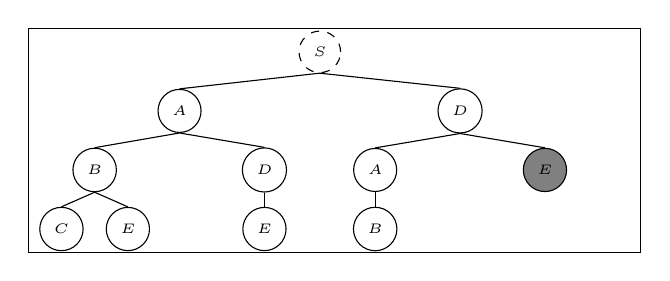
\begin{tikzpicture}[xscale=0.75,yscale=1,city/.style={shape=circle,draw=black},costc/.style={anchor=south east},heurh/.style={anchor=north east,gray},cityG/.style={city,very thick},cityM/.style={city,fill=gray}]
\def\dy{-0.75};
\def\dxa{4.75};
\def\dxb{2.875};
\def\dxc{1.125};
\def\dxd{0.75};
\def\dxe{0.75};

\draw (-0.5*\dxa-0.5*\dxb-\dxc,0.3) rectangle (0.5*\dxa+0.5*\dxb+\dxc+0.5,3*\dy-0.3);

\node[city,dashed] (S) at (0,0) {\tiny $S$};

\node[city] (A) at (-0.5*\dxa,\dy) {\tiny $A$};
\draw (S.south) -- (A.north);
\node[city] (D) at (0.5*\dxa,\dy) {\tiny $D$};
\draw (S.south) -- (D.north);

\node[city] (B) at (-0.5*\dxa-0.5*\dxb,2*\dy) {\tiny $B$};
\draw (A.south) -- (B.north);
\node[city] (D2) at (-0.5*\dxa+0.5*\dxb,2*\dy) {\tiny $D$};
\draw (A.south) -- (D2.north);
\node[city] (A2) at (0.5*\dxa-0.5*\dxb,2*\dy) {\tiny $A$};
\draw (D.south) -- (A2.north);
\node[cityM] (E) at (0.5*\dxa+0.5*\dxb,2*\dy) {\tiny $E$};
\draw (D.south) -- (E.north);

\node[city] (C) at (-0.5*\dxa-0.5*\dxb-0.5*\dxc,3*\dy) {\tiny $C$};
\draw (B.south) -- (C.north);
\node[city] (E2) at (-0.5*\dxa-0.5*\dxb+0.5*\dxc,3*\dy) {\tiny $E$};
\draw (B.south) -- (E2.north);
\node[city] (E3) at (-0.5*\dxa+0.5*\dxb,3*\dy) {\tiny $E$};
\draw (D2.south) -- (E3.north);
\node[city] (B2) at (0.5*\dxa-0.5*\dxb,3*\dy) {\tiny $B$};
\draw (A2.south) -- (B2.north);
\end{tikzpicture}}
\subfigure{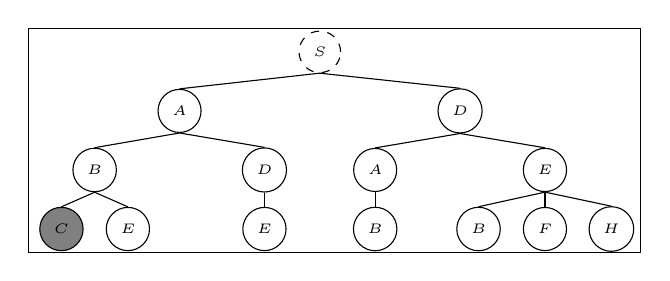
\begin{tikzpicture}[xscale=0.75,yscale=1,city/.style={shape=circle,draw=black},costc/.style={anchor=south east},heurh/.style={anchor=north east,gray},cityG/.style={city,very thick},cityM/.style={city,fill=gray}]
\def\dy{-0.75};
\def\dxa{4.75};
\def\dxb{2.875};
\def\dxc{1.125};
\def\dxd{0.75};
\def\dxe{0.75};

\draw (-0.5*\dxa-0.5*\dxb-\dxc,0.3) rectangle (0.5*\dxa+0.5*\dxb+\dxc+0.5,3*\dy-0.3);

\node[city,dashed] (S) at (0,0) {\tiny $S$};

\node[city] (A) at (-0.5*\dxa,\dy) {\tiny $A$};
\draw (S.south) -- (A.north);
\node[city] (D) at (0.5*\dxa,\dy) {\tiny $D$};
\draw (S.south) -- (D.north);

\node[city] (B) at (-0.5*\dxa-0.5*\dxb,2*\dy) {\tiny $B$};
\draw (A.south) -- (B.north);
\node[city] (D2) at (-0.5*\dxa+0.5*\dxb,2*\dy) {\tiny $D$};
\draw (A.south) -- (D2.north);
\node[city] (A2) at (0.5*\dxa-0.5*\dxb,2*\dy) {\tiny $A$};
\draw (D.south) -- (A2.north);
\node[city] (E) at (0.5*\dxa+0.5*\dxb,2*\dy) {\tiny $E$};
\draw (D.south) -- (E.north);

\node[cityM] (C) at (-0.5*\dxa-0.5*\dxb-0.5*\dxc,3*\dy) {\tiny $C$};
\draw (B.south) -- (C.north);
\node[city] (E2) at (-0.5*\dxa-0.5*\dxb+0.5*\dxc,3*\dy) {\tiny $E$};
\draw (B.south) -- (E2.north);
\node[city] (E3) at (-0.5*\dxa+0.5*\dxb,3*\dy) {\tiny $E$};
\draw (D2.south) -- (E3.north);
\node[city] (B2) at (0.5*\dxa-0.5*\dxb,3*\dy) {\tiny $B$};
\draw (A2.south) -- (B2.north);
\node[city] (B3) at (0.5*\dxa+0.5*\dxb-\dxc,3*\dy) {\tiny $B$};
\draw (E.south) -- (B3.north);
\node[city] (F) at (0.5*\dxa+0.5*\dxb,3*\dy) {\tiny $F$};
\draw (E.south) -- (F.north);
\node[city] (H) at (0.5*\dxa+0.5*\dxb+\dxc,3*\dy) {\tiny $H$};
\draw (E.south) -- (H.north);
\end{tikzpicture}}
\subfigure{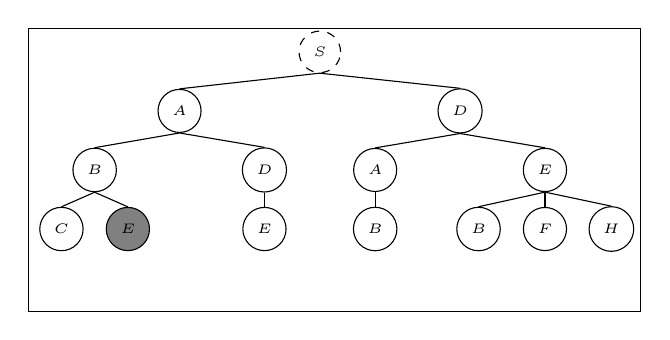
\begin{tikzpicture}[xscale=0.75,yscale=1,city/.style={shape=circle,draw=black},costc/.style={anchor=south east},heurh/.style={anchor=north east,gray},cityG/.style={city,very thick},cityM/.style={city,fill=gray}]
\def\dy{-0.75};
\def\dxa{4.75};
\def\dxb{2.875};
\def\dxc{1.125};
\def\dxd{0.75};
\def\dxe{0.75};

\draw (-0.5*\dxa-0.5*\dxb-\dxc,0.3) rectangle (0.5*\dxa+0.5*\dxb+\dxc+0.5,4*\dy-0.3);

\node[city,dashed] (S) at (0,0) {\tiny $S$};

\node[city] (A) at (-0.5*\dxa,\dy) {\tiny $A$};
\draw (S.south) -- (A.north);
\node[city] (D) at (0.5*\dxa,\dy) {\tiny $D$};
\draw (S.south) -- (D.north);

\node[city] (B) at (-0.5*\dxa-0.5*\dxb,2*\dy) {\tiny $B$};
\draw (A.south) -- (B.north);
\node[city] (D2) at (-0.5*\dxa+0.5*\dxb,2*\dy) {\tiny $D$};
\draw (A.south) -- (D2.north);
\node[city] (A2) at (0.5*\dxa-0.5*\dxb,2*\dy) {\tiny $A$};
\draw (D.south) -- (A2.north);
\node[city] (E) at (0.5*\dxa+0.5*\dxb,2*\dy) {\tiny $E$};
\draw (D.south) -- (E.north);

\node[city] (C) at (-0.5*\dxa-0.5*\dxb-0.5*\dxc,3*\dy) {\tiny $C$};
\draw (B.south) -- (C.north);
\node[cityM] (E2) at (-0.5*\dxa-0.5*\dxb+0.5*\dxc,3*\dy) {\tiny $E$};
\draw (B.south) -- (E2.north);
\node[city] (E3) at (-0.5*\dxa+0.5*\dxb,3*\dy) {\tiny $E$};
\draw (D2.south) -- (E3.north);
\node[city] (B2) at (0.5*\dxa-0.5*\dxb,3*\dy) {\tiny $B$};
\draw (A2.south) -- (B2.north);
\node[city] (B3) at (0.5*\dxa+0.5*\dxb-\dxc,3*\dy) {\tiny $B$};
\draw (E.south) -- (B3.north);
\node[city] (F) at (0.5*\dxa+0.5*\dxb,3*\dy) {\tiny $F$};
\draw (E.south) -- (F.north);
\node[city] (H) at (0.5*\dxa+0.5*\dxb+\dxc,3*\dy) {\tiny $H$};
\draw (E.south) -- (H.north);
\end{tikzpicture}}
\subfigure{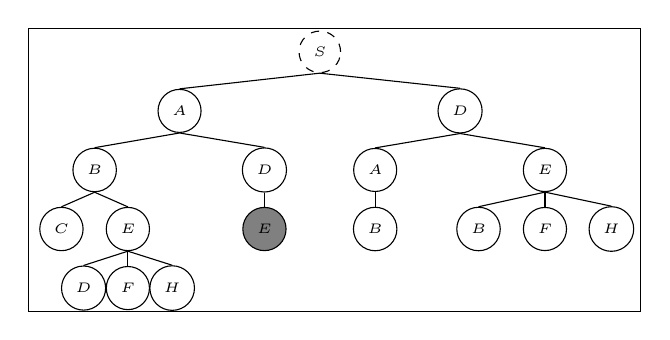
\begin{tikzpicture}[xscale=0.75,yscale=1,city/.style={shape=circle,draw=black},costc/.style={anchor=south east},heurh/.style={anchor=north east,gray},cityG/.style={city,very thick},cityM/.style={city,fill=gray}]
\def\dy{-0.75};
\def\dxa{4.75};
\def\dxb{2.875};
\def\dxc{1.125};
\def\dxd{0.75};
\def\dxe{0.75};

\draw (-0.5*\dxa-0.5*\dxb-\dxc,0.3) rectangle (0.5*\dxa+0.5*\dxb+\dxc+0.5,4*\dy-0.3);

\node[city,dashed] (S) at (0,0) {\tiny $S$};

\node[city] (A) at (-0.5*\dxa,\dy) {\tiny $A$};
\draw (S.south) -- (A.north);
\node[city] (D) at (0.5*\dxa,\dy) {\tiny $D$};
\draw (S.south) -- (D.north);

\node[city] (B) at (-0.5*\dxa-0.5*\dxb,2*\dy) {\tiny $B$};
\draw (A.south) -- (B.north);
\node[city] (D2) at (-0.5*\dxa+0.5*\dxb,2*\dy) {\tiny $D$};
\draw (A.south) -- (D2.north);
\node[city] (A2) at (0.5*\dxa-0.5*\dxb,2*\dy) {\tiny $A$};
\draw (D.south) -- (A2.north);
\node[city] (E) at (0.5*\dxa+0.5*\dxb,2*\dy) {\tiny $E$};
\draw (D.south) -- (E.north);

\node[city] (C) at (-0.5*\dxa-0.5*\dxb-0.5*\dxc,3*\dy) {\tiny $C$};
\draw (B.south) -- (C.north);
\node[city] (E2) at (-0.5*\dxa-0.5*\dxb+0.5*\dxc,3*\dy) {\tiny $E$};
\draw (B.south) -- (E2.north);
\node[cityM] (E3) at (-0.5*\dxa+0.5*\dxb,3*\dy) {\tiny $E$};
\draw (D2.south) -- (E3.north);
\node[city] (B2) at (0.5*\dxa-0.5*\dxb,3*\dy) {\tiny $B$};
\draw (A2.south) -- (B2.north);
\node[city] (B3) at (0.5*\dxa+0.5*\dxb-\dxc,3*\dy) {\tiny $B$};
\draw (E.south) -- (B3.north);
\node[city] (F) at (0.5*\dxa+0.5*\dxb,3*\dy) {\tiny $F$};
\draw (E.south) -- (F.north);
\node[city] (H) at (0.5*\dxa+0.5*\dxb+\dxc,3*\dy) {\tiny $H$};
\draw (E.south) -- (H.north);

\node[city] (D3) at (-0.5*\dxa-0.5*\dxb+0.5*\dxc-\dxd,4*\dy) {\tiny $D$};
\draw (E2.south) -- (D3.north);
\node[city] (F2) at (-0.5*\dxa-0.5*\dxb+0.5*\dxc,4*\dy) {\tiny $F$};
\draw (E2.south) -- (F2.north);
\node[city] (H2) at (-0.5*\dxa-0.5*\dxb+0.5*\dxc+\dxd,4*\dy) {\tiny $H$};
\draw (E2.south) -- (H2.north);
\end{tikzpicture}}
\subfigure{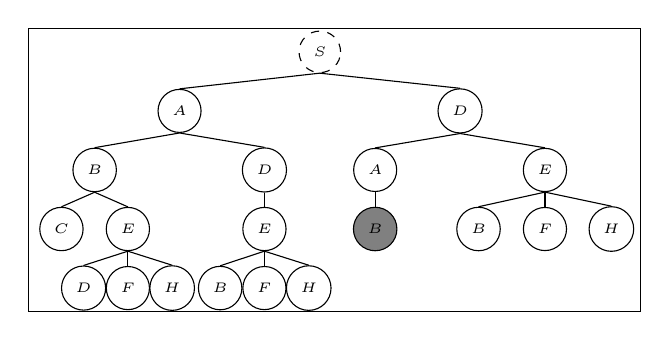
\begin{tikzpicture}[xscale=0.75,yscale=1,city/.style={shape=circle,draw=black},costc/.style={anchor=south east},heurh/.style={anchor=north east,gray},cityG/.style={city,very thick},cityM/.style={city,fill=gray}]
\def\dy{-0.75};
\def\dxa{4.75};
\def\dxb{2.875};
\def\dxc{1.125};
\def\dxd{0.75};
\def\dxe{0.75};

\draw (-0.5*\dxa-0.5*\dxb-\dxc,0.3) rectangle (0.5*\dxa+0.5*\dxb+\dxc+0.5,4*\dy-0.3);

\node[city,dashed] (S) at (0,0) {\tiny $S$};

\node[city] (A) at (-0.5*\dxa,\dy) {\tiny $A$};
\draw (S.south) -- (A.north);
\node[city] (D) at (0.5*\dxa,\dy) {\tiny $D$};
\draw (S.south) -- (D.north);

\node[city] (B) at (-0.5*\dxa-0.5*\dxb,2*\dy) {\tiny $B$};
\draw (A.south) -- (B.north);
\node[city] (D2) at (-0.5*\dxa+0.5*\dxb,2*\dy) {\tiny $D$};
\draw (A.south) -- (D2.north);
\node[city] (A2) at (0.5*\dxa-0.5*\dxb,2*\dy) {\tiny $A$};
\draw (D.south) -- (A2.north);
\node[city] (E) at (0.5*\dxa+0.5*\dxb,2*\dy) {\tiny $E$};
\draw (D.south) -- (E.north);

\node[city] (C) at (-0.5*\dxa-0.5*\dxb-0.5*\dxc,3*\dy) {\tiny $C$};
\draw (B.south) -- (C.north);
\node[city] (E2) at (-0.5*\dxa-0.5*\dxb+0.5*\dxc,3*\dy) {\tiny $E$};
\draw (B.south) -- (E2.north);
\node[city] (E3) at (-0.5*\dxa+0.5*\dxb,3*\dy) {\tiny $E$};
\draw (D2.south) -- (E3.north);
\node[cityM] (B2) at (0.5*\dxa-0.5*\dxb,3*\dy) {\tiny $B$};
\draw (A2.south) -- (B2.north);
\node[city] (B3) at (0.5*\dxa+0.5*\dxb-\dxc,3*\dy) {\tiny $B$};
\draw (E.south) -- (B3.north);
\node[city] (F) at (0.5*\dxa+0.5*\dxb,3*\dy) {\tiny $F$};
\draw (E.south) -- (F.north);
\node[city] (H) at (0.5*\dxa+0.5*\dxb+\dxc,3*\dy) {\tiny $H$};
\draw (E.south) -- (H.north);

\node[city] (D3) at (-0.5*\dxa-0.5*\dxb+0.5*\dxc-\dxd,4*\dy) {\tiny $D$};
\draw (E2.south) -- (D3.north);
\node[city] (F2) at (-0.5*\dxa-0.5*\dxb+0.5*\dxc,4*\dy) {\tiny $F$};
\draw (E2.south) -- (F2.north);
\node[city] (H2) at (-0.5*\dxa-0.5*\dxb+0.5*\dxc+\dxd,4*\dy) {\tiny $H$};
\draw (E2.south) -- (H2.north);
\node[city] (B4) at (-0.5*\dxa+0.5*\dxb-\dxd,4*\dy) {\tiny $B$};
\draw (E3.south) -- (B4.north);
\node[city] (F3) at (-0.5*\dxa+0.5*\dxb,4*\dy) {\tiny $F$};
\draw (E3.south) -- (F3.north);
\node[city] (H3) at (-0.5*\dxa+0.5*\dxb+\dxd,4*\dy) {\tiny $H$};
\draw (E3.south) -- (H3.north);
\end{tikzpicture}}
\subfigure{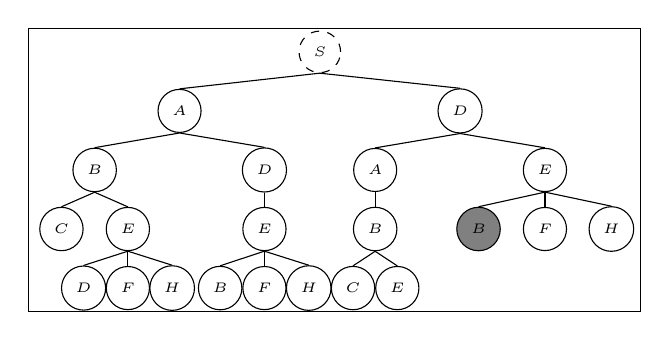
\begin{tikzpicture}[xscale=0.75,yscale=1,city/.style={shape=circle,draw=black},costc/.style={anchor=south east},heurh/.style={anchor=north east,gray},cityG/.style={city,very thick},cityM/.style={city,fill=gray}]
\def\dy{-0.75};
\def\dxa{4.75};
\def\dxb{2.875};
\def\dxc{1.125};
\def\dxd{0.75};
\def\dxe{0.75};

\draw (-0.5*\dxa-0.5*\dxb-\dxc,0.3) rectangle (0.5*\dxa+0.5*\dxb+\dxc+0.5,4*\dy-0.3);

\node[city,dashed] (S) at (0,0) {\tiny $S$};

\node[city] (A) at (-0.5*\dxa,\dy) {\tiny $A$};
\draw (S.south) -- (A.north);
\node[city] (D) at (0.5*\dxa,\dy) {\tiny $D$};
\draw (S.south) -- (D.north);

\node[city] (B) at (-0.5*\dxa-0.5*\dxb,2*\dy) {\tiny $B$};
\draw (A.south) -- (B.north);
\node[city] (D2) at (-0.5*\dxa+0.5*\dxb,2*\dy) {\tiny $D$};
\draw (A.south) -- (D2.north);
\node[city] (A2) at (0.5*\dxa-0.5*\dxb,2*\dy) {\tiny $A$};
\draw (D.south) -- (A2.north);
\node[city] (E) at (0.5*\dxa+0.5*\dxb,2*\dy) {\tiny $E$};
\draw (D.south) -- (E.north);

\node[city] (C) at (-0.5*\dxa-0.5*\dxb-0.5*\dxc,3*\dy) {\tiny $C$};
\draw (B.south) -- (C.north);
\node[city] (E2) at (-0.5*\dxa-0.5*\dxb+0.5*\dxc,3*\dy) {\tiny $E$};
\draw (B.south) -- (E2.north);
\node[city] (E3) at (-0.5*\dxa+0.5*\dxb,3*\dy) {\tiny $E$};
\draw (D2.south) -- (E3.north);
\node[city] (B2) at (0.5*\dxa-0.5*\dxb,3*\dy) {\tiny $B$};
\draw (A2.south) -- (B2.north);
\node[cityM] (B3) at (0.5*\dxa+0.5*\dxb-\dxc,3*\dy) {\tiny $B$};
\draw (E.south) -- (B3.north);
\node[city] (F) at (0.5*\dxa+0.5*\dxb,3*\dy) {\tiny $F$};
\draw (E.south) -- (F.north);
\node[city] (H) at (0.5*\dxa+0.5*\dxb+\dxc,3*\dy) {\tiny $H$};
\draw (E.south) -- (H.north);

\node[city] (D3) at (-0.5*\dxa-0.5*\dxb+0.5*\dxc-\dxd,4*\dy) {\tiny $D$};
\draw (E2.south) -- (D3.north);
\node[city] (F2) at (-0.5*\dxa-0.5*\dxb+0.5*\dxc,4*\dy) {\tiny $F$};
\draw (E2.south) -- (F2.north);
\node[city] (H2) at (-0.5*\dxa-0.5*\dxb+0.5*\dxc+\dxd,4*\dy) {\tiny $H$};
\draw (E2.south) -- (H2.north);
\node[city] (B4) at (-0.5*\dxa+0.5*\dxb-\dxd,4*\dy) {\tiny $B$};
\draw (E3.south) -- (B4.north);
\node[city] (F3) at (-0.5*\dxa+0.5*\dxb,4*\dy) {\tiny $F$};
\draw (E3.south) -- (F3.north);
\node[city] (H3) at (-0.5*\dxa+0.5*\dxb+\dxd,4*\dy) {\tiny $H$};
\draw (E3.south) -- (H3.north);
\node[city] (C2) at (0.5*\dxa-0.5*\dxb-0.5*\dxd,4*\dy) {\tiny $C$};
\draw (B2.south) -- (C2.north);
\node[city] (E4) at (0.5*\dxa-0.5*\dxb+0.5*\dxd,4*\dy) {\tiny $E$};
\draw (B2.south) -- (E4.north);
\end{tikzpicture}}
\subfigure{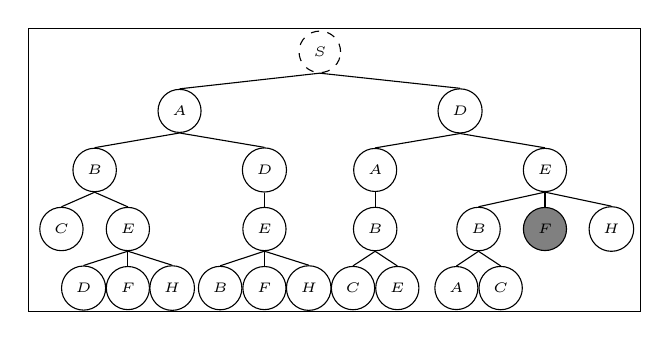
\begin{tikzpicture}[xscale=0.75,yscale=1,city/.style={shape=circle,draw=black},costc/.style={anchor=south east},heurh/.style={anchor=north east,gray},cityG/.style={city,very thick},cityM/.style={city,fill=gray}]
\def\dy{-0.75};
\def\dxa{4.75};
\def\dxb{2.875};
\def\dxc{1.125};
\def\dxd{0.75};
\def\dxe{0.75};

\draw (-0.5*\dxa-0.5*\dxb-\dxc,0.3) rectangle (0.5*\dxa+0.5*\dxb+\dxc+0.5,4*\dy-0.3);

\node[city,dashed] (S) at (0,0) {\tiny $S$};

\node[city] (A) at (-0.5*\dxa,\dy) {\tiny $A$};
\draw (S.south) -- (A.north);
\node[city] (D) at (0.5*\dxa,\dy) {\tiny $D$};
\draw (S.south) -- (D.north);

\node[city] (B) at (-0.5*\dxa-0.5*\dxb,2*\dy) {\tiny $B$};
\draw (A.south) -- (B.north);
\node[city] (D2) at (-0.5*\dxa+0.5*\dxb,2*\dy) {\tiny $D$};
\draw (A.south) -- (D2.north);
\node[city] (A2) at (0.5*\dxa-0.5*\dxb,2*\dy) {\tiny $A$};
\draw (D.south) -- (A2.north);
\node[city] (E) at (0.5*\dxa+0.5*\dxb,2*\dy) {\tiny $E$};
\draw (D.south) -- (E.north);

\node[city] (C) at (-0.5*\dxa-0.5*\dxb-0.5*\dxc,3*\dy) {\tiny $C$};
\draw (B.south) -- (C.north);
\node[city] (E2) at (-0.5*\dxa-0.5*\dxb+0.5*\dxc,3*\dy) {\tiny $E$};
\draw (B.south) -- (E2.north);
\node[city] (E3) at (-0.5*\dxa+0.5*\dxb,3*\dy) {\tiny $E$};
\draw (D2.south) -- (E3.north);
\node[city] (B2) at (0.5*\dxa-0.5*\dxb,3*\dy) {\tiny $B$};
\draw (A2.south) -- (B2.north);
\node[city] (B3) at (0.5*\dxa+0.5*\dxb-\dxc,3*\dy) {\tiny $B$};
\draw (E.south) -- (B3.north);
\node[cityM] (F) at (0.5*\dxa+0.5*\dxb,3*\dy) {\tiny $F$};
\draw (E.south) -- (F.north);
\node[city] (H) at (0.5*\dxa+0.5*\dxb+\dxc,3*\dy) {\tiny $H$};
\draw (E.south) -- (H.north);

\node[city] (D3) at (-0.5*\dxa-0.5*\dxb+0.5*\dxc-\dxd,4*\dy) {\tiny $D$};
\draw (E2.south) -- (D3.north);
\node[city] (F2) at (-0.5*\dxa-0.5*\dxb+0.5*\dxc,4*\dy) {\tiny $F$};
\draw (E2.south) -- (F2.north);
\node[city] (H2) at (-0.5*\dxa-0.5*\dxb+0.5*\dxc+\dxd,4*\dy) {\tiny $H$};
\draw (E2.south) -- (H2.north);
\node[city] (B4) at (-0.5*\dxa+0.5*\dxb-\dxd,4*\dy) {\tiny $B$};
\draw (E3.south) -- (B4.north);
\node[city] (F3) at (-0.5*\dxa+0.5*\dxb,4*\dy) {\tiny $F$};
\draw (E3.south) -- (F3.north);
\node[city] (H3) at (-0.5*\dxa+0.5*\dxb+\dxd,4*\dy) {\tiny $H$};
\draw (E3.south) -- (H3.north);
\node[city] (C2) at (0.5*\dxa-0.5*\dxb-0.5*\dxd,4*\dy) {\tiny $C$};
\draw (B2.south) -- (C2.north);
\node[city] (E4) at (0.5*\dxa-0.5*\dxb+0.5*\dxd,4*\dy) {\tiny $E$};
\draw (B2.south) -- (E4.north);
\node[city] (A3) at (0.5*\dxa+0.5*\dxb-\dxc-0.5*\dxd,4*\dy) {\tiny $A$};
\draw (B3.south) -- (A3.north);
\node[city] (C3) at (0.5*\dxa+0.5*\dxb-\dxc+0.5*\dxd,4*\dy) {\tiny $C$};
\draw (B3.south) -- (C3.north);
\end{tikzpicture}}
\subfigure{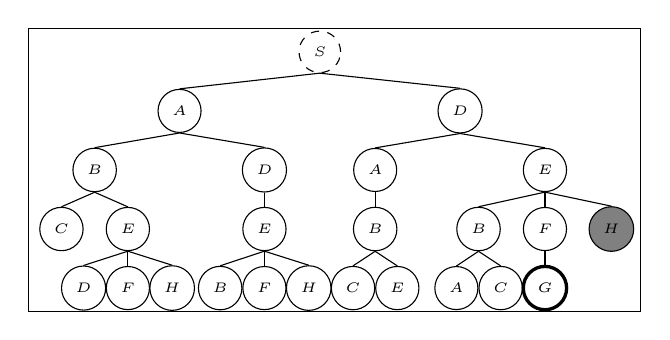
\begin{tikzpicture}[xscale=0.75,yscale=1,city/.style={shape=circle,draw=black},costc/.style={anchor=south east},heurh/.style={anchor=north east,gray},cityG/.style={city,very thick},cityM/.style={city,fill=gray}]
\def\dy{-0.75};
\def\dxa{4.75};
\def\dxb{2.875};
\def\dxc{1.125};
\def\dxd{0.75};
\def\dxe{0.75};

\draw (-0.5*\dxa-0.5*\dxb-\dxc,0.3) rectangle (0.5*\dxa+0.5*\dxb+\dxc+0.5,4*\dy-0.3);

\node[city,dashed] (S) at (0,0) {\tiny $S$};

\node[city] (A) at (-0.5*\dxa,\dy) {\tiny $A$};
\draw (S.south) -- (A.north);
\node[city] (D) at (0.5*\dxa,\dy) {\tiny $D$};
\draw (S.south) -- (D.north);

\node[city] (B) at (-0.5*\dxa-0.5*\dxb,2*\dy) {\tiny $B$};
\draw (A.south) -- (B.north);
\node[city] (D2) at (-0.5*\dxa+0.5*\dxb,2*\dy) {\tiny $D$};
\draw (A.south) -- (D2.north);
\node[city] (A2) at (0.5*\dxa-0.5*\dxb,2*\dy) {\tiny $A$};
\draw (D.south) -- (A2.north);
\node[city] (E) at (0.5*\dxa+0.5*\dxb,2*\dy) {\tiny $E$};
\draw (D.south) -- (E.north);

\node[city] (C) at (-0.5*\dxa-0.5*\dxb-0.5*\dxc,3*\dy) {\tiny $C$};
\draw (B.south) -- (C.north);
\node[city] (E2) at (-0.5*\dxa-0.5*\dxb+0.5*\dxc,3*\dy) {\tiny $E$};
\draw (B.south) -- (E2.north);
\node[city] (E3) at (-0.5*\dxa+0.5*\dxb,3*\dy) {\tiny $E$};
\draw (D2.south) -- (E3.north);
\node[city] (B2) at (0.5*\dxa-0.5*\dxb,3*\dy) {\tiny $B$};
\draw (A2.south) -- (B2.north);
\node[city] (B3) at (0.5*\dxa+0.5*\dxb-\dxc,3*\dy) {\tiny $B$};
\draw (E.south) -- (B3.north);
\node[city] (F) at (0.5*\dxa+0.5*\dxb,3*\dy) {\tiny $F$};
\draw (E.south) -- (F.north);
\node[cityM] (H) at (0.5*\dxa+0.5*\dxb+\dxc,3*\dy) {\tiny $H$};
\draw (E.south) -- (H.north);

\node[city] (D3) at (-0.5*\dxa-0.5*\dxb+0.5*\dxc-\dxd,4*\dy) {\tiny $D$};
\draw (E2.south) -- (D3.north);
\node[city] (F2) at (-0.5*\dxa-0.5*\dxb+0.5*\dxc,4*\dy) {\tiny $F$};
\draw (E2.south) -- (F2.north);
\node[city] (H2) at (-0.5*\dxa-0.5*\dxb+0.5*\dxc+\dxd,4*\dy) {\tiny $H$};
\draw (E2.south) -- (H2.north);
\node[city] (B4) at (-0.5*\dxa+0.5*\dxb-\dxd,4*\dy) {\tiny $B$};
\draw (E3.south) -- (B4.north);
\node[city] (F3) at (-0.5*\dxa+0.5*\dxb,4*\dy) {\tiny $F$};
\draw (E3.south) -- (F3.north);
\node[city] (H3) at (-0.5*\dxa+0.5*\dxb+\dxd,4*\dy) {\tiny $H$};
\draw (E3.south) -- (H3.north);
\node[city] (C2) at (0.5*\dxa-0.5*\dxb-0.5*\dxd,4*\dy) {\tiny $C$};
\draw (B2.south) -- (C2.north);
\node[city] (E4) at (0.5*\dxa-0.5*\dxb+0.5*\dxd,4*\dy) {\tiny $E$};
\draw (B2.south) -- (E4.north);
\node[city] (A3) at (0.5*\dxa+0.5*\dxb-\dxc-0.5*\dxd,4*\dy) {\tiny $A$};
\draw (B3.south) -- (A3.north);
\node[city] (C3) at (0.5*\dxa+0.5*\dxb-\dxc+0.5*\dxd,4*\dy) {\tiny $C$};
\draw (B3.south) -- (C3.north);
\node[cityG] (G) at (0.5*\dxa+0.5*\dxb,4*\dy) {\tiny $G$};
\draw (F.south) -- (G.north);
\end{tikzpicture}}
\caption{Breadth-First toegepast op het wegenplan}
\label{fig:breadthFirstCity}
\end{figure}
\begin{figure}[H]
\centering
\subfigure{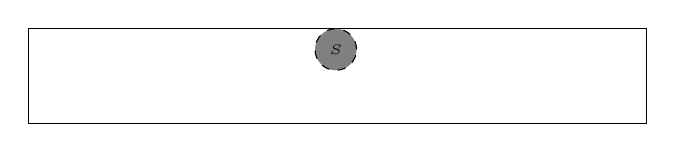
\begin{tikzpicture}[xscale=0.725,yscale=0.9,city/.style={shape=circle,draw=black},cityG/.style={city,very thick},cityM/.style={city,fill=gray}]
\def\dy{-0.75};
\def\dxa{4.75};
\def\dxb{2.875};
\def\dxc{1.125};
\def\dxd{0.75};
\def\dxe{0.75};

\draw (-0.5*\dxa-0.5*\dxb-\dxc-0.45,0.3) rectangle (0.5*\dxa+0.5*\dxb+\dxc+0.5,1*\dy-0.3);

\node[cityM,dashed] (S) at (0,0) {\tiny $S$};

\end{tikzpicture}}
\subfigure{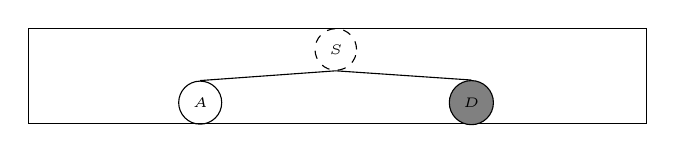
\begin{tikzpicture}[xscale=0.725,yscale=0.9,city/.style={shape=circle,draw=black},cityG/.style={city,very thick},cityM/.style={city,fill=gray}]
\def\dy{-0.75};
\def\dxa{4.75};
\def\dxb{2.875};
\def\dxc{1.125};
\def\dxd{0.75};
\def\dxe{0.75};

\draw (-0.5*\dxa-0.5*\dxb-\dxc-0.45,0.3) rectangle (0.5*\dxa+0.5*\dxb+\dxc+0.5,1*\dy-0.3);

\node[city,dashed] (S) at (0,0) {\tiny $S$};

\node[city] (A) at (-0.5*\dxa,\dy) {\tiny $A$};
\draw (S.south) -- (A.north);
\node[cityM] (D) at (0.5*\dxa,\dy) {\tiny $D$};
\draw (S.south) -- (D.north);

\end{tikzpicture}}
\subfigure{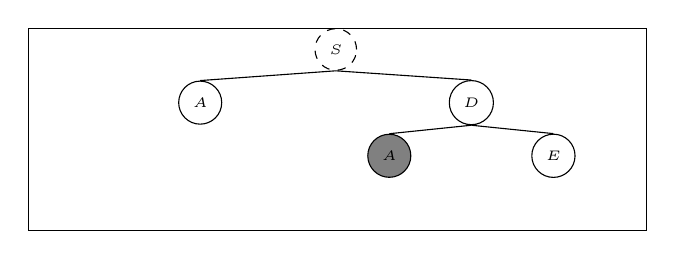
\begin{tikzpicture}[xscale=0.725,yscale=0.9,city/.style={shape=circle,draw=black},cityG/.style={city,very thick},cityM/.style={city,fill=gray}]
\def\dy{-0.75};
\def\dxa{4.75};
\def\dxb{2.875};
\def\dxc{1.125};
\def\dxd{0.75};
\def\dxe{0.75};

\draw (-0.5*\dxa-0.5*\dxb-\dxc-0.45,0.3) rectangle (0.5*\dxa+0.5*\dxb+\dxc+0.5,3*\dy-0.3);

\node[city,dashed] (S) at (0,0) {\tiny $S$};

\node[city] (A) at (-0.5*\dxa,\dy) {\tiny $A$};
\draw (S.south) -- (A.north);
\node[city] (D) at (0.5*\dxa,\dy) {\tiny $D$};
\draw (S.south) -- (D.north);

\node[cityM] (A2) at (0.5*\dxa-0.5*\dxb,2*\dy) {\tiny $A$};
\draw (D.south) -- (A2.north);
\node[city] (E) at (0.5*\dxa+0.5*\dxb,2*\dy) {\tiny $E$};
\draw (D.south) -- (E.north);
\end{tikzpicture}}
\subfigure{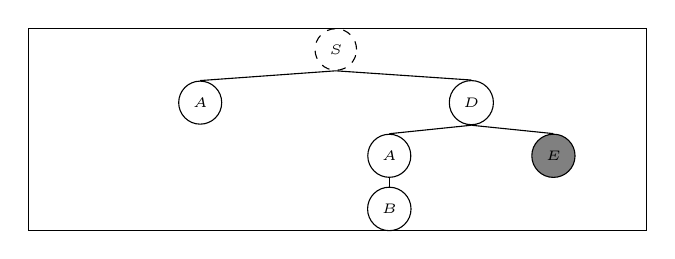
\begin{tikzpicture}[xscale=0.725,yscale=0.9,city/.style={shape=circle,draw=black},cityG/.style={city,very thick},cityM/.style={city,fill=gray}]
\def\dy{-0.75};
\def\dxa{4.75};
\def\dxb{2.875};
\def\dxc{1.125};
\def\dxd{0.75};
\def\dxe{0.75};

\draw (-0.5*\dxa-0.5*\dxb-\dxc-0.45,0.3) rectangle (0.5*\dxa+0.5*\dxb+\dxc+0.5,3*\dy-0.3);

\node[city,dashed] (S) at (0,0) {\tiny $S$};

\node[city] (A) at (-0.5*\dxa,\dy) {\tiny $A$};
\draw (S.south) -- (A.north);
\node[city] (D) at (0.5*\dxa,\dy) {\tiny $D$};
\draw (S.south) -- (D.north);

\node[city] (A2) at (0.5*\dxa-0.5*\dxb,2*\dy) {\tiny $A$};
\draw (D.south) -- (A2.north);
\node[cityM] (E) at (0.5*\dxa+0.5*\dxb,2*\dy) {\tiny $E$};
\draw (D.south) -- (E.north);

\node[city] (B2) at (0.5*\dxa-0.5*\dxb,3*\dy) {\tiny $B$};
\draw (A2.south) -- (B2.north);
\end{tikzpicture}}
\subfigure{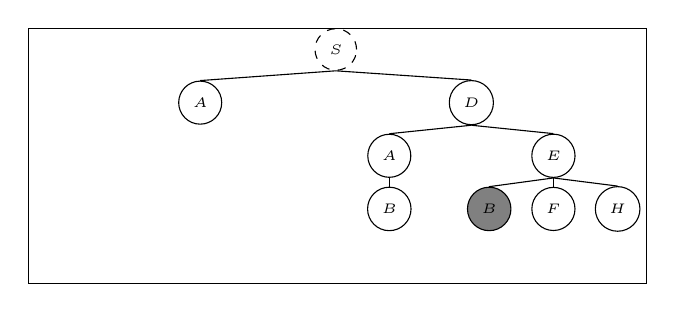
\begin{tikzpicture}[xscale=0.725,yscale=0.9,city/.style={shape=circle,draw=black},cityG/.style={city,very thick},cityM/.style={city,fill=gray}]
\def\dy{-0.75};
\def\dxa{4.75};
\def\dxb{2.875};
\def\dxc{1.125};
\def\dxd{0.75};
\def\dxe{0.75};

\draw (-0.5*\dxa-0.5*\dxb-\dxc-0.45,0.3) rectangle (0.5*\dxa+0.5*\dxb+\dxc+0.5,4*\dy-0.3);

\node[city,dashed] (S) at (0,0) {\tiny $S$};

\node[city] (A) at (-0.5*\dxa,\dy) {\tiny $A$};
\draw (S.south) -- (A.north);
\node[city] (D) at (0.5*\dxa,\dy) {\tiny $D$};
\draw (S.south) -- (D.north);

\node[city] (A2) at (0.5*\dxa-0.5*\dxb,2*\dy) {\tiny $A$};
\draw (D.south) -- (A2.north);
\node[city] (E) at (0.5*\dxa+0.5*\dxb,2*\dy) {\tiny $E$};
\draw (D.south) -- (E.north);

\node[city] (B2) at (0.5*\dxa-0.5*\dxb,3*\dy) {\tiny $B$};
\draw (A2.south) -- (B2.north);
\node[cityM] (B3) at (0.5*\dxa+0.5*\dxb-\dxc,3*\dy) {\tiny $B$};
\draw (E.south) -- (B3.north);
\node[city] (F) at (0.5*\dxa+0.5*\dxb,3*\dy) {\tiny $F$};
\draw (E.south) -- (F.north);
\node[city] (H) at (0.5*\dxa+0.5*\dxb+\dxc,3*\dy) {\tiny $H$};
\draw (E.south) -- (H.north);
\end{tikzpicture}}
\subfigure{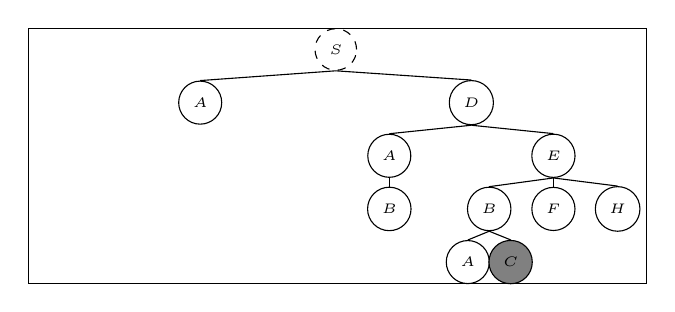
\begin{tikzpicture}[xscale=0.725,yscale=0.9,city/.style={shape=circle,draw=black},cityG/.style={city,very thick},cityM/.style={city,fill=gray}]
\def\dy{-0.75};
\def\dxa{4.75};
\def\dxb{2.875};
\def\dxc{1.125};
\def\dxd{0.75};
\def\dxe{0.75};

\draw (-0.5*\dxa-0.5*\dxb-\dxc-0.45,0.3) rectangle (0.5*\dxa+0.5*\dxb+\dxc+0.5,4*\dy-0.3);

\node[city,dashed] (S) at (0,0) {\tiny $S$};

\node[city] (A) at (-0.5*\dxa,\dy) {\tiny $A$};
\draw (S.south) -- (A.north);
\node[city] (D) at (0.5*\dxa,\dy) {\tiny $D$};
\draw (S.south) -- (D.north);

\node[city] (A2) at (0.5*\dxa-0.5*\dxb,2*\dy) {\tiny $A$};
\draw (D.south) -- (A2.north);
\node[city] (E) at (0.5*\dxa+0.5*\dxb,2*\dy) {\tiny $E$};
\draw (D.south) -- (E.north);

\node[city] (B2) at (0.5*\dxa-0.5*\dxb,3*\dy) {\tiny $B$};
\draw (A2.south) -- (B2.north);
\node[city] (B3) at (0.5*\dxa+0.5*\dxb-\dxc,3*\dy) {\tiny $B$};
\draw (E.south) -- (B3.north);
\node[city] (F) at (0.5*\dxa+0.5*\dxb,3*\dy) {\tiny $F$};
\draw (E.south) -- (F.north);
\node[city] (H) at (0.5*\dxa+0.5*\dxb+\dxc,3*\dy) {\tiny $H$};
\draw (E.south) -- (H.north);

\node[city] (A3) at (0.5*\dxa+0.5*\dxb-\dxc-0.5*\dxd,4*\dy) {\tiny $A$};
\draw (B3.south) -- (A3.north);
\node[cityM] (C3) at (0.5*\dxa+0.5*\dxb-\dxc+0.5*\dxd,4*\dy) {\tiny $C$};
\draw (B3.south) -- (C3.north);
\end{tikzpicture}}
\subfigure{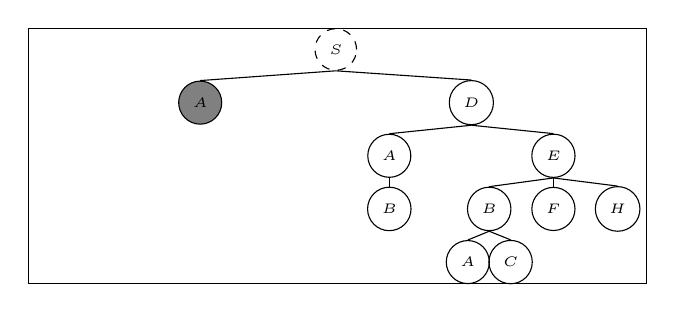
\begin{tikzpicture}[xscale=0.725,yscale=0.9,city/.style={shape=circle,draw=black},cityG/.style={city,very thick},cityM/.style={city,fill=gray}]
\def\dy{-0.75};
\def\dxa{4.75};
\def\dxb{2.875};
\def\dxc{1.125};
\def\dxd{0.75};
\def\dxe{0.75};

\draw (-0.5*\dxa-0.5*\dxb-\dxc-0.45,0.3) rectangle (0.5*\dxa+0.5*\dxb+\dxc+0.5,4*\dy-0.3);

\node[city,dashed] (S) at (0,0) {\tiny $S$};

\node[cityM] (A) at (-0.5*\dxa,\dy) {\tiny $A$};
\draw (S.south) -- (A.north);
\node[city] (D) at (0.5*\dxa,\dy) {\tiny $D$};
\draw (S.south) -- (D.north);

\node[city] (A2) at (0.5*\dxa-0.5*\dxb,2*\dy) {\tiny $A$};
\draw (D.south) -- (A2.north);
\node[city] (E) at (0.5*\dxa+0.5*\dxb,2*\dy) {\tiny $E$};
\draw (D.south) -- (E.north);

\node[city] (B2) at (0.5*\dxa-0.5*\dxb,3*\dy) {\tiny $B$};
\draw (A2.south) -- (B2.north);
\node[city] (B3) at (0.5*\dxa+0.5*\dxb-\dxc,3*\dy) {\tiny $B$};
\draw (E.south) -- (B3.north);
\node[city] (F) at (0.5*\dxa+0.5*\dxb,3*\dy) {\tiny $F$};
\draw (E.south) -- (F.north);
\node[city] (H) at (0.5*\dxa+0.5*\dxb+\dxc,3*\dy) {\tiny $H$};
\draw (E.south) -- (H.north);

\node[city] (A3) at (0.5*\dxa+0.5*\dxb-\dxc-0.5*\dxd,4*\dy) {\tiny $A$};
\draw (B3.south) -- (A3.north);
\node[city] (C3) at (0.5*\dxa+0.5*\dxb-\dxc+0.5*\dxd,4*\dy) {\tiny $C$};
\draw (B3.south) -- (C3.north);
\end{tikzpicture}}
\subfigure{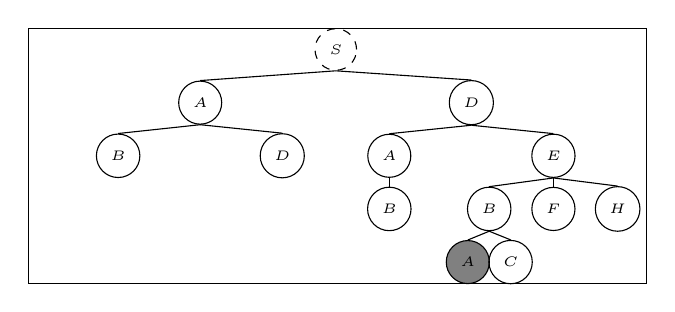
\begin{tikzpicture}[xscale=0.725,yscale=0.9,city/.style={shape=circle,draw=black},cityG/.style={city,very thick},cityM/.style={city,fill=gray}]
\def\dy{-0.75};
\def\dxa{4.75};
\def\dxb{2.875};
\def\dxc{1.125};
\def\dxd{0.75};
\def\dxe{0.75};

\draw (-0.5*\dxa-0.5*\dxb-\dxc-0.45,0.3) rectangle (0.5*\dxa+0.5*\dxb+\dxc+0.5,4*\dy-0.3);

\node[city,dashed] (S) at (0,0) {\tiny $S$};

\node[city] (A) at (-0.5*\dxa,\dy) {\tiny $A$};
\draw (S.south) -- (A.north);
\node[city] (D) at (0.5*\dxa,\dy) {\tiny $D$};
\draw (S.south) -- (D.north);

\node[city] (B) at (-0.5*\dxa-0.5*\dxb,2*\dy) {\tiny $B$};
\draw (A.south) -- (B.north);
\node[city] (D2) at (-0.5*\dxa+0.5*\dxb,2*\dy) {\tiny $D$};
\draw (A.south) -- (D2.north);
\node[city] (A2) at (0.5*\dxa-0.5*\dxb,2*\dy) {\tiny $A$};
\draw (D.south) -- (A2.north);
\node[city] (E) at (0.5*\dxa+0.5*\dxb,2*\dy) {\tiny $E$};
\draw (D.south) -- (E.north);

\node[city] (B2) at (0.5*\dxa-0.5*\dxb,3*\dy) {\tiny $B$};
\draw (A2.south) -- (B2.north);
\node[city] (B3) at (0.5*\dxa+0.5*\dxb-\dxc,3*\dy) {\tiny $B$};
\draw (E.south) -- (B3.north);
\node[city] (F) at (0.5*\dxa+0.5*\dxb,3*\dy) {\tiny $F$};
\draw (E.south) -- (F.north);
\node[city] (H) at (0.5*\dxa+0.5*\dxb+\dxc,3*\dy) {\tiny $H$};
\draw (E.south) -- (H.north);

\node[cityM] (A3) at (0.5*\dxa+0.5*\dxb-\dxc-0.5*\dxd,4*\dy) {\tiny $A$};
\draw (B3.south) -- (A3.north);
\node[city] (C3) at (0.5*\dxa+0.5*\dxb-\dxc+0.5*\dxd,4*\dy) {\tiny $C$};
\draw (B3.south) -- (C3.north);
\end{tikzpicture}}
\subfigure{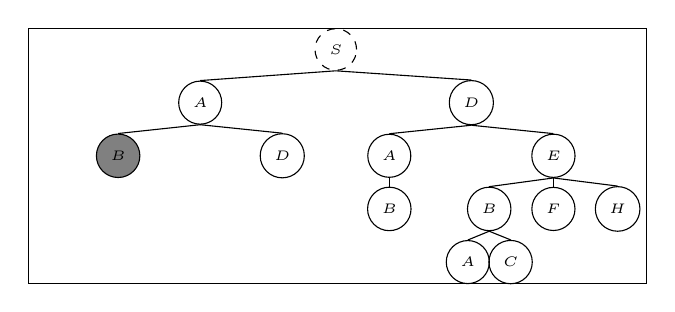
\begin{tikzpicture}[xscale=0.725,yscale=0.9,city/.style={shape=circle,draw=black},cityG/.style={city,very thick},cityM/.style={city,fill=gray}]
\def\dy{-0.75};
\def\dxa{4.75};
\def\dxb{2.875};
\def\dxc{1.125};
\def\dxd{0.75};
\def\dxe{0.75};

\draw (-0.5*\dxa-0.5*\dxb-\dxc-0.45,0.3) rectangle (0.5*\dxa+0.5*\dxb+\dxc+0.5,4*\dy-0.3);

\node[city,dashed] (S) at (0,0) {\tiny $S$};

\node[city] (A) at (-0.5*\dxa,\dy) {\tiny $A$};
\draw (S.south) -- (A.north);
\node[city] (D) at (0.5*\dxa,\dy) {\tiny $D$};
\draw (S.south) -- (D.north);

\node[cityM] (B) at (-0.5*\dxa-0.5*\dxb,2*\dy) {\tiny $B$};
\draw (A.south) -- (B.north);
\node[city] (D2) at (-0.5*\dxa+0.5*\dxb,2*\dy) {\tiny $D$};
\draw (A.south) -- (D2.north);
\node[city] (A2) at (0.5*\dxa-0.5*\dxb,2*\dy) {\tiny $A$};
\draw (D.south) -- (A2.north);
\node[city] (E) at (0.5*\dxa+0.5*\dxb,2*\dy) {\tiny $E$};
\draw (D.south) -- (E.north);

\node[city] (B2) at (0.5*\dxa-0.5*\dxb,3*\dy) {\tiny $B$};
\draw (A2.south) -- (B2.north);
\node[city] (B3) at (0.5*\dxa+0.5*\dxb-\dxc,3*\dy) {\tiny $B$};
\draw (E.south) -- (B3.north);
\node[city] (F) at (0.5*\dxa+0.5*\dxb,3*\dy) {\tiny $F$};
\draw (E.south) -- (F.north);
\node[city] (H) at (0.5*\dxa+0.5*\dxb+\dxc,3*\dy) {\tiny $H$};
\draw (E.south) -- (H.north);

\node[city] (A3) at (0.5*\dxa+0.5*\dxb-\dxc-0.5*\dxd,4*\dy) {\tiny $A$};
\draw (B3.south) -- (A3.north);
\node[city] (C3) at (0.5*\dxa+0.5*\dxb-\dxc+0.5*\dxd,4*\dy) {\tiny $C$};
\draw (B3.south) -- (C3.north);
\end{tikzpicture}}
\subfigure{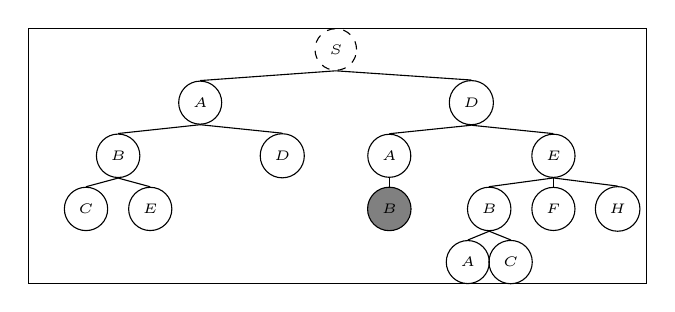
\begin{tikzpicture}[xscale=0.725,yscale=0.9,city/.style={shape=circle,draw=black},cityG/.style={city,very thick},cityM/.style={city,fill=gray}]
\def\dy{-0.75};
\def\dxa{4.75};
\def\dxb{2.875};
\def\dxc{1.125};
\def\dxd{0.75};
\def\dxe{0.75};

\draw (-0.5*\dxa-0.5*\dxb-\dxc-0.45,0.3) rectangle (0.5*\dxa+0.5*\dxb+\dxc+0.5,4*\dy-0.3);

\node[city,dashed] (S) at (0,0) {\tiny $S$};

\node[city] (A) at (-0.5*\dxa,\dy) {\tiny $A$};
\draw (S.south) -- (A.north);
\node[city] (D) at (0.5*\dxa,\dy) {\tiny $D$};
\draw (S.south) -- (D.north);

\node[city] (B) at (-0.5*\dxa-0.5*\dxb,2*\dy) {\tiny $B$};
\draw (A.south) -- (B.north);
\node[city] (D2) at (-0.5*\dxa+0.5*\dxb,2*\dy) {\tiny $D$};
\draw (A.south) -- (D2.north);
\node[city] (A2) at (0.5*\dxa-0.5*\dxb,2*\dy) {\tiny $A$};
\draw (D.south) -- (A2.north);
\node[city] (E) at (0.5*\dxa+0.5*\dxb,2*\dy) {\tiny $E$};
\draw (D.south) -- (E.north);

\node[city] (C) at (-0.5*\dxa-0.5*\dxb-0.5*\dxc,3*\dy) {\tiny $C$};
\draw (B.south) -- (C.north);
\node[city] (E2) at (-0.5*\dxa-0.5*\dxb+0.5*\dxc,3*\dy) {\tiny $E$};
\draw (B.south) -- (E2.north);
\node[cityM] (B2) at (0.5*\dxa-0.5*\dxb,3*\dy) {\tiny $B$};
\draw (A2.south) -- (B2.north);
\node[city] (B3) at (0.5*\dxa+0.5*\dxb-\dxc,3*\dy) {\tiny $B$};
\draw (E.south) -- (B3.north);
\node[city] (F) at (0.5*\dxa+0.5*\dxb,3*\dy) {\tiny $F$};
\draw (E.south) -- (F.north);
\node[city] (H) at (0.5*\dxa+0.5*\dxb+\dxc,3*\dy) {\tiny $H$};
\draw (E.south) -- (H.north);

\node[city] (A3) at (0.5*\dxa+0.5*\dxb-\dxc-0.5*\dxd,4*\dy) {\tiny $A$};
\draw (B3.south) -- (A3.north);
\node[city] (C3) at (0.5*\dxa+0.5*\dxb-\dxc+0.5*\dxd,4*\dy) {\tiny $C$};
\draw (B3.south) -- (C3.north);
\end{tikzpicture}}
\subfigure{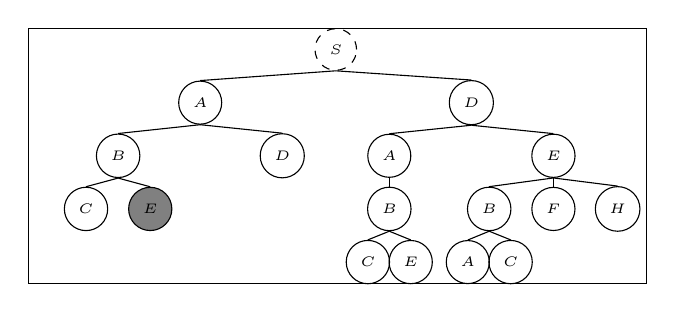
\begin{tikzpicture}[xscale=0.725,yscale=0.9,city/.style={shape=circle,draw=black},cityG/.style={city,very thick},cityM/.style={city,fill=gray}]
\def\dy{-0.75};
\def\dxa{4.75};
\def\dxb{2.875};
\def\dxc{1.125};
\def\dxd{0.75};
\def\dxe{0.75};

\draw (-0.5*\dxa-0.5*\dxb-\dxc-0.45,0.3) rectangle (0.5*\dxa+0.5*\dxb+\dxc+0.5,4*\dy-0.3);

\node[city,dashed] (S) at (0,0) {\tiny $S$};

\node[city] (A) at (-0.5*\dxa,\dy) {\tiny $A$};
\draw (S.south) -- (A.north);
\node[city] (D) at (0.5*\dxa,\dy) {\tiny $D$};
\draw (S.south) -- (D.north);

\node[city] (B) at (-0.5*\dxa-0.5*\dxb,2*\dy) {\tiny $B$};
\draw (A.south) -- (B.north);
\node[city] (D2) at (-0.5*\dxa+0.5*\dxb,2*\dy) {\tiny $D$};
\draw (A.south) -- (D2.north);
\node[city] (A2) at (0.5*\dxa-0.5*\dxb,2*\dy) {\tiny $A$};
\draw (D.south) -- (A2.north);
\node[city] (E) at (0.5*\dxa+0.5*\dxb,2*\dy) {\tiny $E$};
\draw (D.south) -- (E.north);

\node[city] (C) at (-0.5*\dxa-0.5*\dxb-0.5*\dxc,3*\dy) {\tiny $C$};
\draw (B.south) -- (C.north);
\node[cityM] (E2) at (-0.5*\dxa-0.5*\dxb+0.5*\dxc,3*\dy) {\tiny $E$};
\draw (B.south) -- (E2.north);
\node[city] (B2) at (0.5*\dxa-0.5*\dxb,3*\dy) {\tiny $B$};
\draw (A2.south) -- (B2.north);
\node[city] (B3) at (0.5*\dxa+0.5*\dxb-\dxc,3*\dy) {\tiny $B$};
\draw (E.south) -- (B3.north);
\node[city] (F) at (0.5*\dxa+0.5*\dxb,3*\dy) {\tiny $F$};
\draw (E.south) -- (F.north);
\node[city] (H) at (0.5*\dxa+0.5*\dxb+\dxc,3*\dy) {\tiny $H$};
\draw (E.south) -- (H.north);

\node[city] (C2) at (0.5*\dxa-0.5*\dxb-0.5*\dxd,4*\dy) {\tiny $C$};
\draw (B2.south) -- (C2.north);
\node[city] (E4) at (0.5*\dxa-0.5*\dxb+0.5*\dxd,4*\dy) {\tiny $E$};
\draw (B2.south) -- (E4.north);
\node[city] (A3) at (0.5*\dxa+0.5*\dxb-\dxc-0.5*\dxd,4*\dy) {\tiny $A$};
\draw (B3.south) -- (A3.north);
\node[city] (C3) at (0.5*\dxa+0.5*\dxb-\dxc+0.5*\dxd,4*\dy) {\tiny $C$};
\draw (B3.south) -- (C3.north);
\end{tikzpicture}}
\subfigure{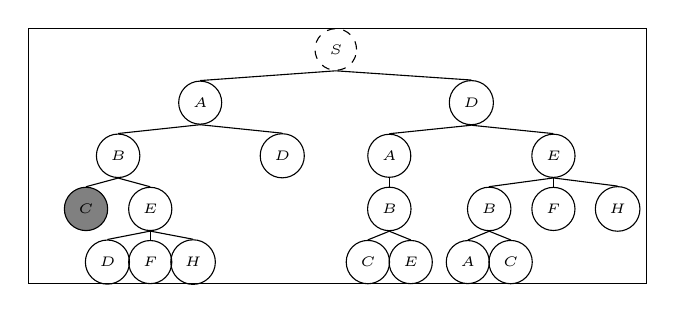
\begin{tikzpicture}[xscale=0.725,yscale=0.9,city/.style={shape=circle,draw=black},cityG/.style={city,very thick},cityM/.style={city,fill=gray}]
\def\dy{-0.75};
\def\dxa{4.75};
\def\dxb{2.875};
\def\dxc{1.125};
\def\dxd{0.75};
\def\dxe{0.75};

\draw (-0.5*\dxa-0.5*\dxb-\dxc-0.45,0.3) rectangle (0.5*\dxa+0.5*\dxb+\dxc+0.5,4*\dy-0.3);

\node[city,dashed] (S) at (0,0) {\tiny $S$};

\node[city] (A) at (-0.5*\dxa,\dy) {\tiny $A$};
\draw (S.south) -- (A.north);
\node[city] (D) at (0.5*\dxa,\dy) {\tiny $D$};
\draw (S.south) -- (D.north);

\node[city] (B) at (-0.5*\dxa-0.5*\dxb,2*\dy) {\tiny $B$};
\draw (A.south) -- (B.north);
\node[city] (D2) at (-0.5*\dxa+0.5*\dxb,2*\dy) {\tiny $D$};
\draw (A.south) -- (D2.north);
\node[city] (A2) at (0.5*\dxa-0.5*\dxb,2*\dy) {\tiny $A$};
\draw (D.south) -- (A2.north);
\node[city] (E) at (0.5*\dxa+0.5*\dxb,2*\dy) {\tiny $E$};
\draw (D.south) -- (E.north);

\node[cityM] (C) at (-0.5*\dxa-0.5*\dxb-0.5*\dxc,3*\dy) {\tiny $C$};
\draw (B.south) -- (C.north);
\node[city] (E2) at (-0.5*\dxa-0.5*\dxb+0.5*\dxc,3*\dy) {\tiny $E$};
\draw (B.south) -- (E2.north);
\node[city] (B2) at (0.5*\dxa-0.5*\dxb,3*\dy) {\tiny $B$};
\draw (A2.south) -- (B2.north);
\node[city] (B3) at (0.5*\dxa+0.5*\dxb-\dxc,3*\dy) {\tiny $B$};
\draw (E.south) -- (B3.north);
\node[city] (F) at (0.5*\dxa+0.5*\dxb,3*\dy) {\tiny $F$};
\draw (E.south) -- (F.north);
\node[city] (H) at (0.5*\dxa+0.5*\dxb+\dxc,3*\dy) {\tiny $H$};
\draw (E.south) -- (H.north);

\node[city] (D3) at (-0.5*\dxa-0.5*\dxb+0.5*\dxc-\dxd,4*\dy) {\tiny $D$};
\draw (E2.south) -- (D3.north);
\node[city] (F2) at (-0.5*\dxa-0.5*\dxb+0.5*\dxc,4*\dy) {\tiny $F$};
\draw (E2.south) -- (F2.north);
\node[city] (H2) at (-0.5*\dxa-0.5*\dxb+0.5*\dxc+\dxd,4*\dy) {\tiny $H$};
\draw (E2.south) -- (H2.north);
\node[city] (C2) at (0.5*\dxa-0.5*\dxb-0.5*\dxd,4*\dy) {\tiny $C$};
\draw (B2.south) -- (C2.north);
\node[city] (E4) at (0.5*\dxa-0.5*\dxb+0.5*\dxd,4*\dy) {\tiny $E$};
\draw (B2.south) -- (E4.north);
\node[city] (A3) at (0.5*\dxa+0.5*\dxb-\dxc-0.5*\dxd,4*\dy) {\tiny $A$};
\draw (B3.south) -- (A3.north);
\node[city] (C3) at (0.5*\dxa+0.5*\dxb-\dxc+0.5*\dxd,4*\dy) {\tiny $C$};
\draw (B3.south) -- (C3.north);
\end{tikzpicture}}
\subfigure{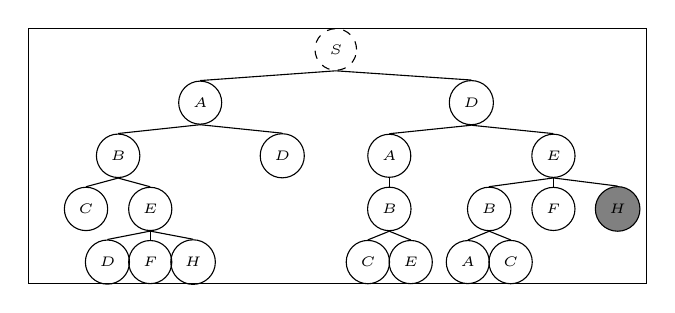
\begin{tikzpicture}[xscale=0.725,yscale=0.9,city/.style={shape=circle,draw=black},cityG/.style={city,very thick},cityM/.style={city,fill=gray}]
\def\dy{-0.75};
\def\dxa{4.75};
\def\dxb{2.875};
\def\dxc{1.125};
\def\dxd{0.75};
\def\dxe{0.75};

\draw (-0.5*\dxa-0.5*\dxb-\dxc-0.45,0.3) rectangle (0.5*\dxa+0.5*\dxb+\dxc+0.5,4*\dy-0.3);

\node[city,dashed] (S) at (0,0) {\tiny $S$};

\node[city] (A) at (-0.5*\dxa,\dy) {\tiny $A$};
\draw (S.south) -- (A.north);
\node[city] (D) at (0.5*\dxa,\dy) {\tiny $D$};
\draw (S.south) -- (D.north);

\node[city] (B) at (-0.5*\dxa-0.5*\dxb,2*\dy) {\tiny $B$};
\draw (A.south) -- (B.north);
\node[city] (D2) at (-0.5*\dxa+0.5*\dxb,2*\dy) {\tiny $D$};
\draw (A.south) -- (D2.north);
\node[city] (A2) at (0.5*\dxa-0.5*\dxb,2*\dy) {\tiny $A$};
\draw (D.south) -- (A2.north);
\node[city] (E) at (0.5*\dxa+0.5*\dxb,2*\dy) {\tiny $E$};
\draw (D.south) -- (E.north);

\node[city] (C) at (-0.5*\dxa-0.5*\dxb-0.5*\dxc,3*\dy) {\tiny $C$};
\draw (B.south) -- (C.north);
\node[city] (E2) at (-0.5*\dxa-0.5*\dxb+0.5*\dxc,3*\dy) {\tiny $E$};
\draw (B.south) -- (E2.north);
\node[city] (B2) at (0.5*\dxa-0.5*\dxb,3*\dy) {\tiny $B$};
\draw (A2.south) -- (B2.north);
\node[city] (B3) at (0.5*\dxa+0.5*\dxb-\dxc,3*\dy) {\tiny $B$};
\draw (E.south) -- (B3.north);
\node[city] (F) at (0.5*\dxa+0.5*\dxb,3*\dy) {\tiny $F$};
\draw (E.south) -- (F.north);
\node[cityM] (H) at (0.5*\dxa+0.5*\dxb+\dxc,3*\dy) {\tiny $H$};
\draw (E.south) -- (H.north);

\node[city] (D3) at (-0.5*\dxa-0.5*\dxb+0.5*\dxc-\dxd,4*\dy) {\tiny $D$};
\draw (E2.south) -- (D3.north);
\node[city] (F2) at (-0.5*\dxa-0.5*\dxb+0.5*\dxc,4*\dy) {\tiny $F$};
\draw (E2.south) -- (F2.north);
\node[city] (H2) at (-0.5*\dxa-0.5*\dxb+0.5*\dxc+\dxd,4*\dy) {\tiny $H$};
\draw (E2.south) -- (H2.north);
\node[city] (C2) at (0.5*\dxa-0.5*\dxb-0.5*\dxd,4*\dy) {\tiny $C$};
\draw (B2.south) -- (C2.north);
\node[city] (E4) at (0.5*\dxa-0.5*\dxb+0.5*\dxd,4*\dy) {\tiny $E$};
\draw (B2.south) -- (E4.north);
\node[city] (A3) at (0.5*\dxa+0.5*\dxb-\dxc-0.5*\dxd,4*\dy) {\tiny $A$};
\draw (B3.south) -- (A3.north);
\node[city] (C3) at (0.5*\dxa+0.5*\dxb-\dxc+0.5*\dxd,4*\dy) {\tiny $C$};
\draw (B3.south) -- (C3.north);
\end{tikzpicture}}
\subfigure{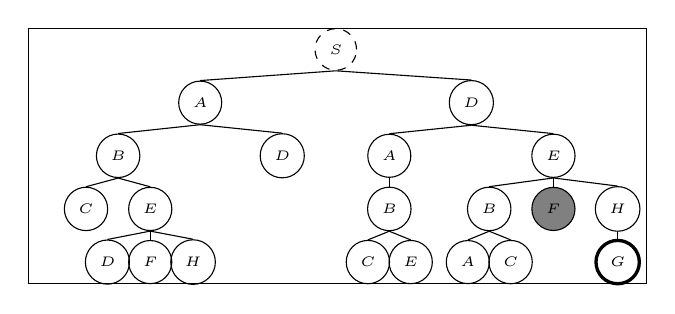
\begin{tikzpicture}[xscale=0.725,yscale=0.9,city/.style={shape=circle,draw=black},cityG/.style={city,very thick},cityM/.style={city,fill=gray}]
\def\dy{-0.75};
\def\dxa{4.75};
\def\dxb{2.875};
\def\dxc{1.125};
\def\dxd{0.75};
\def\dxe{0.75};

\draw (-0.5*\dxa-0.5*\dxb-\dxc-0.45,0.3) rectangle (0.5*\dxa+0.5*\dxb+\dxc+0.5,4*\dy-0.3);

\node[city,dashed] (S) at (0,0) {\tiny $S$};

\node[city] (A) at (-0.5*\dxa,\dy) {\tiny $A$};
\draw (S.south) -- (A.north);
\node[city] (D) at (0.5*\dxa,\dy) {\tiny $D$};
\draw (S.south) -- (D.north);

\node[city] (B) at (-0.5*\dxa-0.5*\dxb,2*\dy) {\tiny $B$};
\draw (A.south) -- (B.north);
\node[city] (D2) at (-0.5*\dxa+0.5*\dxb,2*\dy) {\tiny $D$};
\draw (A.south) -- (D2.north);
\node[city] (A2) at (0.5*\dxa-0.5*\dxb,2*\dy) {\tiny $A$};
\draw (D.south) -- (A2.north);
\node[city] (E) at (0.5*\dxa+0.5*\dxb,2*\dy) {\tiny $E$};
\draw (D.south) -- (E.north);

\node[city] (C) at (-0.5*\dxa-0.5*\dxb-0.5*\dxc,3*\dy) {\tiny $C$};
\draw (B.south) -- (C.north);
\node[city] (E2) at (-0.5*\dxa-0.5*\dxb+0.5*\dxc,3*\dy) {\tiny $E$};
\draw (B.south) -- (E2.north);
\node[city] (B2) at (0.5*\dxa-0.5*\dxb,3*\dy) {\tiny $B$};
\draw (A2.south) -- (B2.north);
\node[city] (B3) at (0.5*\dxa+0.5*\dxb-\dxc,3*\dy) {\tiny $B$};
\draw (E.south) -- (B3.north);
\node[cityM] (F) at (0.5*\dxa+0.5*\dxb,3*\dy) {\tiny $F$};
\draw (E.south) -- (F.north);
\node[city] (H) at (0.5*\dxa+0.5*\dxb+\dxc,3*\dy) {\tiny $H$};
\draw (E.south) -- (H.north);

\node[city] (D3) at (-0.5*\dxa-0.5*\dxb+0.5*\dxc-\dxd,4*\dy) {\tiny $D$};
\draw (E2.south) -- (D3.north);
\node[city] (F2) at (-0.5*\dxa-0.5*\dxb+0.5*\dxc,4*\dy) {\tiny $F$};
\draw (E2.south) -- (F2.north);
\node[city] (H2) at (-0.5*\dxa-0.5*\dxb+0.5*\dxc+\dxd,4*\dy) {\tiny $H$};
\draw (E2.south) -- (H2.north);
\node[city] (C2) at (0.5*\dxa-0.5*\dxb-0.5*\dxd,4*\dy) {\tiny $C$};
\draw (B2.south) -- (C2.north);
\node[city] (E4) at (0.5*\dxa-0.5*\dxb+0.5*\dxd,4*\dy) {\tiny $E$};
\draw (B2.south) -- (E4.north);
\node[city] (A3) at (0.5*\dxa+0.5*\dxb-\dxc-0.5*\dxd,4*\dy) {\tiny $A$};
\draw (B3.south) -- (A3.north);
\node[city] (C3) at (0.5*\dxa+0.5*\dxb-\dxc+0.5*\dxd,4*\dy) {\tiny $C$};
\draw (B3.south) -- (C3.north);
\node[cityG] (G2) at (0.5*\dxa+0.5*\dxb+\dxc,4*\dy) {\tiny $G$};
\draw (H.south) -- (G2.north);
\end{tikzpicture}}
\caption{Een mogelijk scenario van Non-Deterministic Search toegepast op het wegenplan}
\label{fig:nonDeterministicCity}
\end{figure}

\subsubsection{Heuristic Search Methods}
\begin{figure}[H]
\centering
\subfigure{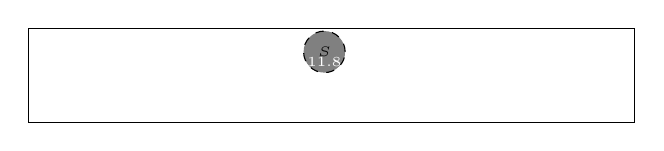
\begin{tikzpicture}[xscale=0.725,yscale=.8,city/.style={shape=circle,draw=black},heurh/.style={yshift=4,gray},heurhM/.style={heurh,white},cityG/.style={city,very thick},cityM/.style={city,fill=gray}]
\def\dy{-0.75};
\def\dxa{4.75};
\def\dxb{2.875};
\def\dxc{1.125};
\def\dxd{0.75};
\def\dxe{0.75};

\draw (-0.5*\dxa-0.5*\dxb-\dxc-0.25,0.375) rectangle (0.5*\dxa+0.5*\dxb+\dxc+0.5,1*\dy-0.375);

\node[cityM,dashed] (S) at (0,0) {\tiny $S$};
\node[heurhM] (Sh) at (S.south) {\tiny 11.8};
\end{tikzpicture}}
\subfigure{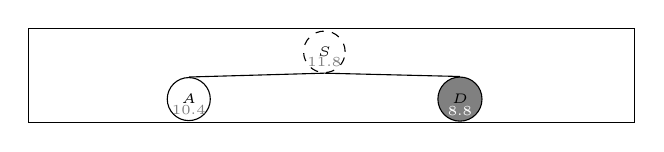
\begin{tikzpicture}[xscale=0.725,yscale=.8,city/.style={shape=circle,draw=black},heurh/.style={yshift=4,gray},heurhM/.style={heurh,white},cityG/.style={city,very thick},cityM/.style={city,fill=gray}]
\def\dy{-0.75};
\def\dxa{4.75};
\def\dxb{2.875};
\def\dxc{1.125};
\def\dxd{0.75};
\def\dxe{0.75};

\draw (-0.5*\dxa-0.5*\dxb-\dxc-0.25,0.375) rectangle (0.5*\dxa+0.5*\dxb+\dxc+0.5,1*\dy-0.375);

\node[city,dashed] (S) at (0,0) {\tiny $S$};
\node[heurh] (Sh) at (S.south) {\tiny 11.8};

\node[city] (A) at (-0.5*\dxa,\dy) {\tiny $A$};
\node[heurh] (Ah) at (A.south) {\tiny 10.4};
\draw (S.south) -- (A.north);
\node[cityM] (D) at (0.5*\dxa,\dy) {\tiny $D$};
\node[heurhM] (Dh) at (D.south) {\tiny 8.8};
\draw (S.south) -- (D.north);
\end{tikzpicture}}
\subfigure{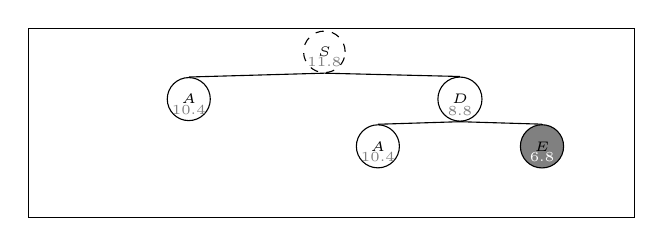
\begin{tikzpicture}[xscale=0.725,yscale=.8,city/.style={shape=circle,draw=black},heurh/.style={yshift=4,gray},heurhM/.style={heurh,white},cityG/.style={city,very thick},cityM/.style={city,fill=gray}]
\def\dy{-0.75};
\def\dxa{4.75};
\def\dxb{2.875};
\def\dxc{1.125};
\def\dxd{0.75};
\def\dxe{0.75};

\draw (-0.5*\dxa-0.5*\dxb-\dxc-0.25,0.375) rectangle (0.5*\dxa+0.5*\dxb+\dxc+0.5,3*\dy-0.375);

\node[city,dashed] (S) at (0,0) {\tiny $S$};
\node[heurh] (Sh) at (S.south) {\tiny 11.8};

\node[city] (A) at (-0.5*\dxa,\dy) {\tiny $A$};
\node[heurh] (Ah) at (A.south) {\tiny 10.4};
\draw (S.south) -- (A.north);
\node[city] (D) at (0.5*\dxa,\dy) {\tiny $D$};
\node[heurh] (Dh) at (D.south) {\tiny 8.8};
\draw (S.south) -- (D.north);

\node[city] (A2) at (0.5*\dxa-0.5*\dxb,2*\dy) {\tiny $A$};
\node[heurh] (A2h) at (A2.south) {\tiny 10.4};
\draw (D.south) -- (A2.north);
\node[cityM] (E) at (0.5*\dxa+0.5*\dxb,2*\dy) {\tiny $E$};
\node[heurhM] (Eh) at (E.south) {\tiny 6.8};
\draw (D.south) -- (E.north);
\end{tikzpicture}}
\subfigure{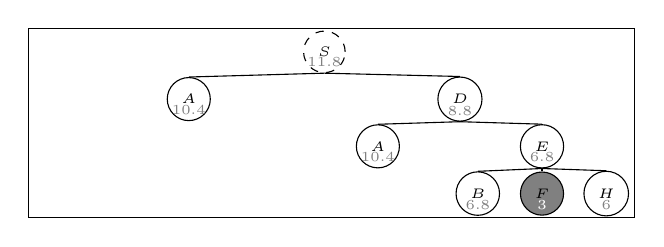
\begin{tikzpicture}[xscale=0.725,yscale=.8,city/.style={shape=circle,draw=black},heurh/.style={yshift=4,gray},heurhM/.style={heurh,white},cityG/.style={city,very thick},cityM/.style={city,fill=gray}]
\def\dy{-0.75};
\def\dxa{4.75};
\def\dxb{2.875};
\def\dxc{1.125};
\def\dxd{0.75};
\def\dxe{0.75};

\draw (-0.5*\dxa-0.5*\dxb-\dxc-0.25,0.375) rectangle (0.5*\dxa+0.5*\dxb+\dxc+0.5,3*\dy-0.375);

\node[city,dashed] (S) at (0,0) {\tiny $S$};
\node[heurh] (Sh) at (S.south) {\tiny 11.8};

\node[city] (A) at (-0.5*\dxa,\dy) {\tiny $A$};
\node[heurh] (Ah) at (A.south) {\tiny 10.4};
\draw (S.south) -- (A.north);
\node[city] (D) at (0.5*\dxa,\dy) {\tiny $D$};
\node[heurh] (Dh) at (D.south) {\tiny 8.8};
\draw (S.south) -- (D.north);

\node[city] (A2) at (0.5*\dxa-0.5*\dxb,2*\dy) {\tiny $A$};
\node[heurh] (A2h) at (A2.south) {\tiny 10.4};
\draw (D.south) -- (A2.north);
\node[city] (E) at (0.5*\dxa+0.5*\dxb,2*\dy) {\tiny $E$};
\node[heurh] (Eh) at (E.south) {\tiny 6.8};
\draw (D.south) -- (E.north);

\node[city] (B3) at (0.5*\dxa+0.5*\dxb-\dxc,3*\dy) {\tiny $B$};
\node[heurh] (B3h) at (B3.south) {\tiny 6.8};
\draw (E.south) -- (B3.north);
\node[cityM] (F) at (0.5*\dxa+0.5*\dxb,3*\dy) {\tiny $F$};
\node[heurhM] (Fh) at (F.south) {\tiny 3};
\draw (E.south) -- (F.north);
\node[city] (H) at (0.5*\dxa+0.5*\dxb+\dxc,3*\dy) {\tiny $H$};
\node[heurh] (Hh) at (H.south) {\tiny 6};
\draw (E.south) -- (H.north);
\end{tikzpicture}}
\subfigure{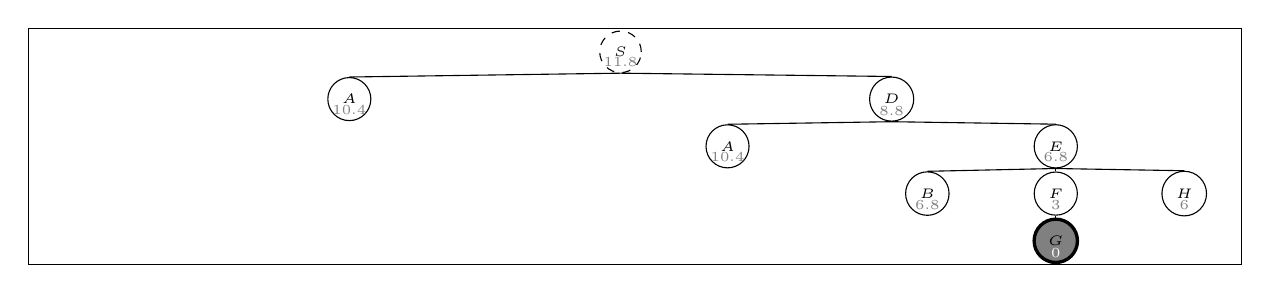
\begin{tikzpicture}[xscale=1.45,yscale=.8,city/.style={shape=circle,draw=black},heurh/.style={yshift=4,gray},heurhM/.style={heurh,white},cityG/.style={city,very thick},cityM/.style={city,fill=gray}]
\def\dy{-0.75};
\def\dxa{4.75};
\def\dxb{2.875};
\def\dxc{1.125};
\def\dxd{0.75};
\def\dxe{0.75};

\draw (-0.5*\dxa-0.5*\dxb-\dxc-0.25,0.375) rectangle (0.5*\dxa+0.5*\dxb+\dxc+0.5,4*\dy-0.375);

\node[city,dashed] (S) at (0,0) {\tiny $S$};
\node[heurh] (Sh) at (S.south) {\tiny 11.8};

\node[city] (A) at (-0.5*\dxa,\dy) {\tiny $A$};
\node[heurh] (Ah) at (A.south) {\tiny 10.4};
\draw (S.south) -- (A.north);
\node[city] (D) at (0.5*\dxa,\dy) {\tiny $D$};
\node[heurh] (Dh) at (D.south) {\tiny 8.8};
\draw (S.south) -- (D.north);

\node[city] (A2) at (0.5*\dxa-0.5*\dxb,2*\dy) {\tiny $A$};
\node[heurh] (A2h) at (A2.south) {\tiny 10.4};
\draw (D.south) -- (A2.north);
\node[city] (E) at (0.5*\dxa+0.5*\dxb,2*\dy) {\tiny $E$};
\node[heurh] (Eh) at (E.south) {\tiny 6.8};
\draw (D.south) -- (E.north);

\node[city] (B3) at (0.5*\dxa+0.5*\dxb-\dxc,3*\dy) {\tiny $B$};
\node[heurh] (B3h) at (B3.south) {\tiny 6.8};
\draw (E.south) -- (B3.north);
\node[city] (F) at (0.5*\dxa+0.5*\dxb,3*\dy) {\tiny $F$};
\node[heurh] (Fh) at (F.south) {\tiny 3};
\draw (E.south) -- (F.north);
\node[city] (H) at (0.5*\dxa+0.5*\dxb+\dxc,3*\dy) {\tiny $H$};
\node[heurh] (Hh) at (H.south) {\tiny 6};
\draw (E.south) -- (H.north);

\node[cityM,cityG] (G) at (0.5*\dxa+0.5*\dxb,4*\dy) {\tiny $G$};
\node[heurhM] (Gh) at (G.south) {\tiny 0};
\draw (F.south) -- (G.north);
\end{tikzpicture}}
\caption{Hill Climbing toegepast op het wegenplan}
\label{fig:hillClimbingCity}
\end{figure}
\begin{figure}[H]
\centering
\subfigure{\begin{tikzpicture}[xscale=0.725,yscale=.8,city/.style={shape=circle,draw=black},heurh/.style={yshift=4,gray},heurhM/.style={heurh,white},cityG/.style={city,very thick},cityM/.style={city,fill=gray}]
\def\dy{-0.75};
\def\dxa{4.75};
\def\dxb{2.875};
\def\dxc{1.125};
\def\dxd{0.75};
\def\dxe{0.75};

\draw (-0.5*\dxa-0.5*\dxb-\dxc-0.25,0.375) rectangle (0.5*\dxa+0.5*\dxb+\dxc+0.5,1*\dy-0.375);

\node[cityM,dashed] (S) at (0,0) {\tiny $S$};
\node[heurhM] (Sh) at (S.south) {\tiny 11.8};
\end{tikzpicture}}
\subfigure{\begin{tikzpicture}[xscale=0.725,yscale=.8,city/.style={shape=circle,draw=black},heurh/.style={yshift=4,gray},heurhM/.style={heurh,white},cityG/.style={city,very thick},cityM/.style={city,fill=gray}]
\def\dy{-0.75};
\def\dxa{4.75};
\def\dxb{2.875};
\def\dxc{1.125};
\def\dxd{0.75};
\def\dxe{0.75};

\draw (-0.5*\dxa-0.5*\dxb-\dxc-0.25,0.375) rectangle (0.5*\dxa+0.5*\dxb+\dxc+0.5,1*\dy-0.375);

\node[city,dashed] (S) at (0,0) {\tiny $S$};
\node[heurh] (Sh) at (S.south) {\tiny 11.8};

\node[cityM] (A) at (-0.5*\dxa,\dy) {\tiny $A$};
\node[heurhM] (Ah) at (A.south) {\tiny 10.4};
\draw (S.south) -- (A.north);
\node[city] (D) at (0.5*\dxa,\dy) {\tiny $D$};
\node[heurh] (Dh) at (D.south) {\tiny 8.8};
\draw (S.south) -- (D.north);
\end{tikzpicture}}
\subfigure{\begin{tikzpicture}[xscale=0.725,yscale=.8,city/.style={shape=circle,draw=black},heurh/.style={yshift=4,gray},heurhM/.style={heurh,white},cityG/.style={city,very thick},cityM/.style={city,fill=gray}]
\def\dy{-0.75};
\def\dxa{4.75};
\def\dxb{2.875};
\def\dxc{1.125};
\def\dxd{0.75};
\def\dxe{0.75};

\draw (-0.5*\dxa-0.5*\dxb-\dxc-0.25,0.375) rectangle (0.5*\dxa+0.5*\dxb+\dxc+0.5,2*\dy-0.375);

\node[city,dashed] (S) at (0,0) {\tiny $S$};
\node[heurh] (Sh) at (S.south) {\tiny 11.8};

\node[city] (A) at (-0.5*\dxa,\dy) {\tiny $A$};
\node[heurh] (Ah) at (A.south) {\tiny 10.4};
\draw (S.south) -- (A.north);
\node[cityM] (D) at (0.5*\dxa,\dy) {\tiny $D$};
\node[heurhM] (Dh) at (D.south) {\tiny 8.8};
\draw (S.south) -- (D.north);

\node[city] (B) at (-0.5*\dxa-0.5*\dxb,2*\dy) {\tiny $B$};
\node[heurh] (Bh) at (B.south) {\tiny 6.8};
\draw (A.south) -- (B.north);
\node[city] (D2) at (-0.5*\dxa+0.5*\dxb,2*\dy) {\tiny $D$};
\node[heurh] (D2h) at (D2.south) {\tiny 8.8};
\draw (A.south) -- (D2.north);
\end{tikzpicture}}
\subfigure{\begin{tikzpicture}[xscale=0.725,yscale=.8,city/.style={shape=circle,draw=black},heurh/.style={yshift=4,gray},heurhM/.style={heurh,white},cityG/.style={city,very thick},cityM/.style={city,fill=gray}]
\def\dy{-0.75};
\def\dxa{4.75};
\def\dxb{2.875};
\def\dxc{1.125};
\def\dxd{0.75};
\def\dxe{0.75};

\draw (-0.5*\dxa-0.5*\dxb-\dxc-0.25,0.375) rectangle (0.5*\dxa+0.5*\dxb+\dxc+0.5,2*\dy-0.375);

\node[city,dashed] (S) at (0,0) {\tiny $S$};
\node[heurh] (Sh) at (S.south) {\tiny 11.8};

\node[city] (A) at (-0.5*\dxa,\dy) {\tiny $A$};
\node[heurh] (Ah) at (A.south) {\tiny 10.4};
\draw (S.south) -- (A.north);
\node[city] (D) at (0.5*\dxa,\dy) {\tiny $D$};
\node[heurh] (Dh) at (D.south) {\tiny 8.8};
\draw (S.south) -- (D.north);

\node[cityM] (B) at (-0.5*\dxa-0.5*\dxb,2*\dy) {\tiny $B$};
\node[heurhM] (Bh) at (B.south) {\tiny 6.8};
\draw (A.south) -- (B.north);
\node[city] (D2) at (-0.5*\dxa+0.5*\dxb,2*\dy) {\tiny $D$};
\node[heurh] (D2h) at (D2.south) {\tiny 8.8};
\draw (A.south) -- (D2.north);
\draw[very thick] (D2.north east) -- (D2.south west);
\draw[very thick] (D2.north west) -- (D2.south east);
\node[city] (A2) at (0.5*\dxa-0.5*\dxb,2*\dy) {\tiny $A$};
\node[heurh] (A2h) at (A2.south) {\tiny 10.4};
\draw (D.south) -- (A2.north);
\draw[very thick] (A2.north east) -- (A2.south west);
\draw[very thick] (A2.north west) -- (A2.south east);
\node[city] (E) at (0.5*\dxa+0.5*\dxb,2*\dy) {\tiny $E$};
\node[heurh] (Eh) at (E.south) {\tiny 6.8};
\draw (D.south) -- (E.north);
\end{tikzpicture}}
\subfigure{\begin{tikzpicture}[xscale=0.725,yscale=.8,city/.style={shape=circle,draw=black},heurh/.style={yshift=4,gray},heurhM/.style={heurh,white},cityG/.style={city,very thick},cityM/.style={city,fill=gray}]
\def\dy{-0.75};
\def\dxa{4.75};
\def\dxb{2.875};
\def\dxc{1.125};
\def\dxd{0.75};
\def\dxe{0.75};

\draw (-0.5*\dxa-0.5*\dxb-\dxc-0.25,0.375) rectangle (0.5*\dxa+0.5*\dxb+\dxc+0.5,3*\dy-0.375);

\node[city,dashed] (S) at (0,0) {\tiny $S$};
\node[heurh] (Sh) at (S.south) {\tiny 11.8};

\node[city] (A) at (-0.5*\dxa,\dy) {\tiny $A$};
\node[heurh] (Ah) at (A.south) {\tiny 10.4};
\draw (S.south) -- (A.north);
\node[city] (D) at (0.5*\dxa,\dy) {\tiny $D$};
\node[heurh] (Dh) at (D.south) {\tiny 8.8};
\draw (S.south) -- (D.north);

\node[city] (B) at (-0.5*\dxa-0.5*\dxb,2*\dy) {\tiny $B$};
\node[heurh] (Bh) at (B.south) {\tiny 6.8};
\draw (A.south) -- (B.north);
\node[cityM] (E) at (0.5*\dxa+0.5*\dxb,2*\dy) {\tiny $E$};
\node[heurhM] (Eh) at (E.south) {\tiny 6.8};
\draw (D.south) -- (E.north);

\node[city] (C) at (-0.5*\dxa-0.5*\dxb-0.5*\dxc,3*\dy) {\tiny $C$};
\node[heurh] (Ch) at (C.south) {\tiny 4};
\draw (B.south) -- (C.north);
\node[city] (E2) at (-0.5*\dxa-0.5*\dxb+0.5*\dxc,3*\dy) {\tiny $E$};
\node[heurh] (E2h) at (E2.south) {\tiny 6.8};
\draw (B.south) -- (E2.north);
\end{tikzpicture}}
\subfigure{\begin{tikzpicture}[xscale=0.725,yscale=.8,city/.style={shape=circle,draw=black},heurh/.style={yshift=4,gray},heurhM/.style={heurh,white},cityG/.style={city,very thick},cityM/.style={city,fill=gray}]
\def\dy{-0.75};
\def\dxa{4.75};
\def\dxb{2.875};
\def\dxc{1.125};
\def\dxd{0.75};
\def\dxe{0.75};

\draw (-0.5*\dxa-0.5*\dxb-\dxc-0.25,0.375) rectangle (0.5*\dxa+0.5*\dxb+\dxc+0.5,3*\dy-0.375);

\node[city,dashed] (S) at (0,0) {\tiny $S$};
\node[heurh] (Sh) at (S.south) {\tiny 11.8};

\node[city] (A) at (-0.5*\dxa,\dy) {\tiny $A$};
\node[heurh] (Ah) at (A.south) {\tiny 10.4};
\draw (S.south) -- (A.north);
\node[city] (D) at (0.5*\dxa,\dy) {\tiny $D$};
\node[heurh] (Dh) at (D.south) {\tiny 8.8};
\draw (S.south) -- (D.north);

\node[city] (B) at (-0.5*\dxa-0.5*\dxb,2*\dy) {\tiny $B$};
\node[heurh] (Bh) at (B.south) {\tiny 6.8};
\draw (A.south) -- (B.north);
\node[city] (E) at (0.5*\dxa+0.5*\dxb,2*\dy) {\tiny $E$};
\node[heurh] (Eh) at (E.south) {\tiny 6.8};
\draw (D.south) -- (E.north);

\node[cityM] (C) at (-0.5*\dxa-0.5*\dxb-0.5*\dxc,3*\dy) {\tiny $C$};
\node[heurhM] (Ch) at (C.south) {\tiny 4};
\draw (B.south) -- (C.north);
\node[city] (E2) at (-0.5*\dxa-0.5*\dxb+0.5*\dxc,3*\dy) {\tiny $E$};
\node[heurh] (E2h) at (E2.south) {\tiny 6.8};
\draw (B.south) -- (E2.north);
\draw[very thick] (E2.north east) -- (E2.south west);
\draw[very thick] (E2.north west) -- (E2.south east);
\node[city] (B3) at (0.5*\dxa+0.5*\dxb-\dxc,3*\dy) {\tiny $B$};
\node[heurh] (B3h) at (B3.south) {\tiny 6.8};
\draw (E.south) -- (B3.north);
\draw[very thick] (B3.north east) -- (B3.south west);
\draw[very thick] (B3.north west) -- (B3.south east);
\node[city] (F) at (0.5*\dxa+0.5*\dxb,3*\dy) {\tiny $F$};
\node[heurh] (Fh) at (F.south) {\tiny 3};
\draw (E.south) -- (F.north);
\node[city] (H) at (0.5*\dxa+0.5*\dxb+\dxc,3*\dy) {\tiny $H$};
\node[heurh] (Hh) at (H.south) {\tiny 6};
\draw (E.south) -- (H.north);
\draw[very thick] (H.north east) -- (H.south west);
\draw[very thick] (H.north west) -- (H.south east);
\end{tikzpicture}}
\subfigure{\begin{tikzpicture}[xscale=0.725,yscale=.8,city/.style={shape=circle,draw=black},heurh/.style={yshift=4,gray},heurhM/.style={heurh,white},cityG/.style={city,very thick},cityM/.style={city,fill=gray}]
\def\dy{-0.75};
\def\dxa{4.75};
\def\dxb{2.875};
\def\dxc{1.125};
\def\dxd{0.75};
\def\dxe{0.75};

\draw (-0.5*\dxa-0.5*\dxb-\dxc-0.25,0.375) rectangle (0.5*\dxa+0.5*\dxb+\dxc+0.5,4*\dy-0.375);

\node[city,dashed] (S) at (0,0) {\tiny $S$};
\node[heurh] (Sh) at (S.south) {\tiny 11.8};

\node[city] (A) at (-0.5*\dxa,\dy) {\tiny $A$};
\node[heurh] (Ah) at (A.south) {\tiny 10.4};
\draw (S.south) -- (A.north);
\node[city] (D) at (0.5*\dxa,\dy) {\tiny $D$};
\node[heurh] (Dh) at (D.south) {\tiny 8.8};
\draw (S.south) -- (D.north);

\node[city] (B) at (-0.5*\dxa-0.5*\dxb,2*\dy) {\tiny $B$};
\node[heurh] (Bh) at (B.south) {\tiny 6.8};
\draw (A.south) -- (B.north);
\node[city] (E) at (0.5*\dxa+0.5*\dxb,2*\dy) {\tiny $E$};
\node[heurh] (Eh) at (E.south) {\tiny 6.8};
\draw (D.south) -- (E.north);

\node[city] (C) at (-0.5*\dxa-0.5*\dxb-0.5*\dxc,3*\dy) {\tiny $C$};
\node[heurh] (Ch) at (C.south) {\tiny 4};
\draw (B.south) -- (C.north);
\node[cityM] (F) at (0.5*\dxa+0.5*\dxb,3*\dy) {\tiny $F$};
\node[heurhM] (Fh) at (F.south) {\tiny 3};
\draw (E.south) -- (F.north);
\end{tikzpicture}}
\subfigure{\begin{tikzpicture}[xscale=0.725,yscale=.8,city/.style={shape=circle,draw=black},heurh/.style={yshift=4,gray},heurhM/.style={heurh,white},cityG/.style={city,very thick},cityM/.style={city,fill=gray}]
\def\dy{-0.75};
\def\dxa{4.75};
\def\dxb{2.875};
\def\dxc{1.125};
\def\dxd{0.75};
\def\dxe{0.75};

\draw (-0.5*\dxa-0.5*\dxb-\dxc-0.25,0.375) rectangle (0.5*\dxa+0.5*\dxb+\dxc+0.5,4*\dy-0.375);

\node[city,dashed] (S) at (0,0) {\tiny $S$};
\node[heurh] (Sh) at (S.south) {\tiny 11.8};

\node[city] (A) at (-0.5*\dxa,\dy) {\tiny $A$};
\node[heurh] (Ah) at (A.south) {\tiny 10.4};
\draw (S.south) -- (A.north);
\node[city] (D) at (0.5*\dxa,\dy) {\tiny $D$};
\node[heurh] (Dh) at (D.south) {\tiny 8.8};
\draw (S.south) -- (D.north);

\node[city] (B) at (-0.5*\dxa-0.5*\dxb,2*\dy) {\tiny $B$};
\node[heurh] (Bh) at (B.south) {\tiny 6.8};
\draw (A.south) -- (B.north);
\node[city] (E) at (0.5*\dxa+0.5*\dxb,2*\dy) {\tiny $E$};
\node[heurh] (Eh) at (E.south) {\tiny 6.8};
\draw (D.south) -- (E.north);

\node[city] (C) at (-0.5*\dxa-0.5*\dxb-0.5*\dxc,3*\dy) {\tiny $C$};
\node[heurh] (Ch) at (C.south) {\tiny 4};
\draw (B.south) -- (C.north);
\node[city] (F) at (0.5*\dxa+0.5*\dxb,3*\dy) {\tiny $F$};
\node[heurh] (Fh) at (F.south) {\tiny 3};
\draw (E.south) -- (F.north);

\node[cityM,cityG] (G) at (0.5*\dxa+0.5*\dxb,4*\dy) {\tiny $G$};
\node[heurhM] (Gh) at (G.south) {\tiny 0};
\draw (F.south) -- (G.north);
\end{tikzpicture}}
\caption{Beam Search toegepast op het wegenplan (met $w=2$)}
\label{fig:beamSearchCity}
\end{figure}
\begin{figure}[H]
\centering
\subfigure{\begin{tikzpicture}[xscale=0.725,yscale=.8,city/.style={shape=circle,draw=black},heurh/.style={yshift=4,gray},heurhM/.style={heurh,white},cityG/.style={city,very thick},cityM/.style={city,fill=gray}]
\def\dy{-0.75};
\def\dxa{4.75};
\def\dxb{2.875};
\def\dxc{1.125};
\def\dxd{0.75};
\def\dxe{0.75};

\draw (-0.5*\dxa-0.5*\dxb-\dxc-0.25,0.375) rectangle (0.5*\dxa+0.5*\dxb+\dxc+0.5,1*\dy-0.375);

\node[cityM,dashed] (S) at (0,0) {\tiny $S$};
\node[heurhM] (Sh) at (S.south) {\tiny 11.8};
\end{tikzpicture}}
\subfigure{\begin{tikzpicture}[xscale=0.725,yscale=.8,city/.style={shape=circle,draw=black},heurh/.style={yshift=4,gray},heurhM/.style={heurh,white},cityG/.style={city,very thick},cityM/.style={city,fill=gray}]
\def\dy{-0.75};
\def\dxa{4.75};
\def\dxb{2.875};
\def\dxc{1.125};
\def\dxd{0.75};
\def\dxe{0.75};

\draw (-0.5*\dxa-0.5*\dxb-\dxc-0.25,0.375) rectangle (0.5*\dxa+0.5*\dxb+\dxc+0.5,1*\dy-0.375);

\node[city,dashed] (S) at (0,0) {\tiny $S$};
\node[heurh] (Sh) at (S.south) {\tiny 11.8};

\node[city] (A) at (-0.5*\dxa,\dy) {\tiny $A$};
\node[heurh] (Ah) at (A.south) {\tiny 10.4};
\draw (S.south) -- (A.north);
\draw[very thick] (A.north east) -- (A.south west);
\draw[very thick] (A.north west) -- (A.south east);
\node[cityM] (D) at (0.5*\dxa,\dy) {\tiny $D$};
\node[heurhM] (Dh) at (D.south) {\tiny 8.8};
\draw (S.south) -- (D.north);
\end{tikzpicture}}
\subfigure{\begin{tikzpicture}[xscale=0.725,yscale=.8,city/.style={shape=circle,draw=black},heurh/.style={yshift=4,gray},heurhM/.style={heurh,white},cityG/.style={city,very thick},cityM/.style={city,fill=gray}]
\def\dy{-0.75};
\def\dxa{4.75};
\def\dxb{2.875};
\def\dxc{1.125};
\def\dxd{0.75};
\def\dxe{0.75};

\draw (-0.5*\dxa-0.5*\dxb-\dxc-0.25,0.375) rectangle (0.5*\dxa+0.5*\dxb+\dxc+0.5,3*\dy-0.375);

\node[city,dashed] (S) at (0,0) {\tiny $S$};
\node[heurh] (Sh) at (S.south) {\tiny 11.8};

\node[city] (D) at (0.5*\dxa,\dy) {\tiny $D$};
\node[heurh] (Dh) at (D.south) {\tiny 8.8};
\draw (S.south) -- (D.north);

\node[city] (A2) at (0.5*\dxa-0.5*\dxb,2*\dy) {\tiny $A$};
\node[heurh] (A2h) at (A2.south) {\tiny 10.4};
\draw (D.south) -- (A2.north);
\draw[very thick] (A2.north east) -- (A2.south west);
\draw[very thick] (A2.north west) -- (A2.south east);
\node[cityM] (E) at (0.5*\dxa+0.5*\dxb,2*\dy) {\tiny $E$};
\node[heurhM] (Eh) at (E.south) {\tiny 6.8};
\draw (D.south) -- (E.north);
\end{tikzpicture}}
\subfigure{\begin{tikzpicture}[xscale=0.725,yscale=.8,city/.style={shape=circle,draw=black},heurh/.style={yshift=4,gray},heurhM/.style={heurh,white},cityG/.style={city,very thick},cityM/.style={city,fill=gray}]
\def\dy{-0.75};
\def\dxa{4.75};
\def\dxb{2.875};
\def\dxc{1.125};
\def\dxd{0.75};
\def\dxe{0.75};

\draw (-0.5*\dxa-0.5*\dxb-\dxc-0.25,0.375) rectangle (0.5*\dxa+0.5*\dxb+\dxc+0.5,3*\dy-0.375);

\node[city,dashed] (S) at (0,0) {\tiny $S$};
\node[heurh] (Sh) at (S.south) {\tiny 11.8};

\node[city] (D) at (0.5*\dxa,\dy) {\tiny $D$};
\node[heurh] (Dh) at (D.south) {\tiny 8.8};
\draw (S.south) -- (D.north);

\node[city] (E) at (0.5*\dxa+0.5*\dxb,2*\dy) {\tiny $E$};
\node[heurh] (Eh) at (E.south) {\tiny 6.8};
\draw (D.south) -- (E.north);

\node[city] (B3) at (0.5*\dxa+0.5*\dxb-\dxc,3*\dy) {\tiny $B$};
\node[heurh] (B3h) at (B3.south) {\tiny 6.8};
\draw (E.south) -- (B3.north);
\draw[very thick] (B3.north east) -- (B3.south west);
\draw[very thick] (B3.north west) -- (B3.south east);
\node[cityM] (F) at (0.5*\dxa+0.5*\dxb,3*\dy) {\tiny $F$};
\node[heurhM] (Fh) at (F.south) {\tiny 3};
\draw (E.south) -- (F.north);
\node[city] (H) at (0.5*\dxa+0.5*\dxb+\dxc,3*\dy) {\tiny $H$};
\node[heurh] (Hh) at (H.south) {\tiny 6};
\draw (E.south) -- (H.north);
\draw[very thick] (H.north east) -- (H.south west);
\draw[very thick] (H.north west) -- (H.south east);
\end{tikzpicture}}
\subfigure{\begin{tikzpicture}[xscale=1.45,yscale=.8,city/.style={shape=circle,draw=black},heurh/.style={yshift=4,gray},heurhM/.style={heurh,white},cityG/.style={city,very thick},cityM/.style={city,fill=gray}]
\def\dy{-0.75};
\def\dxa{4.75};
\def\dxb{2.875};
\def\dxc{1.125};
\def\dxd{0.75};
\def\dxe{0.75};

\draw (-0.5*\dxa-0.5*\dxb-\dxc-0.25,0.375) rectangle (0.5*\dxa+0.5*\dxb+\dxc+0.5,4*\dy-0.375);

\node[city,dashed] (S) at (0,0) {\tiny $S$};
\node[heurh] (Sh) at (S.south) {\tiny 11.8};

\node[city] (D) at (0.5*\dxa,\dy) {\tiny $D$};
\node[heurh] (Dh) at (D.south) {\tiny 8.8};
\draw (S.south) -- (D.north);

\node[city] (E) at (0.5*\dxa+0.5*\dxb,2*\dy) {\tiny $E$};
\node[heurh] (Eh) at (E.south) {\tiny 6.8};
\draw (D.south) -- (E.north);

\node[city] (F) at (0.5*\dxa+0.5*\dxb,3*\dy) {\tiny $F$};
\node[heurh] (Fh) at (F.south) {\tiny 3};
\draw (E.south) -- (F.north);

\node[cityM,cityG] (G) at (0.5*\dxa+0.5*\dxb,4*\dy) {\tiny $G$};
\node[heurhM] (Gh) at (G.south) {\tiny 0};
\draw (F.south) -- (G.north);
\end{tikzpicture}}
\caption{Hill Climbing 2 toegepast op het wegenplan}
\label{fig:hillClimbing2City}
\end{figure}
\subsubsection{Optimal Search Methods}
\begin{figure}[H]
\subfigure{\begin{tikzpicture}[xscale=0.725,yscale=0.9,city/.style={shape=circle,draw=black},costc/.style={yshift=-3},heurh/.style={anchor=north east,gray},cityG/.style={city,very thick},cityM/.style={city,fill=gray}]
\def\dy{-0.75};
\def\dxa{4.75};
\def\dxb{2.875};
\def\dxc{1.125};
\def\dxd{0.75};
\def\dxe{0.75};

\draw (-0.5*\dxa-0.5*\dxb-\dxc-0.45,0.3) rectangle (0.5*\dxa+0.5*\dxb+\dxc+0.5,1*\dy-0.3);

\node[cityM,dashed] (S) at (0,0) {\tiny $S$};
\node[costc] (Sc) at (S.north) {\tiny 0};

\end{tikzpicture}}
\subfigure{\begin{tikzpicture}[xscale=0.725,yscale=0.9,city/.style={shape=circle,draw=black},costc/.style={yshift=-3},heurh/.style={anchor=north east,gray},cityG/.style={city,very thick},cityM/.style={city,fill=gray}]
\def\dy{-0.75};
\def\dxa{4.75};
\def\dxb{2.875};
\def\dxc{1.125};
\def\dxd{0.75};
\def\dxe{0.75};

\draw (-0.5*\dxa-0.5*\dxb-\dxc-0.45,0.3) rectangle (0.5*\dxa+0.5*\dxb+\dxc+0.5,1*\dy-0.3);

\node[city,dashed] (S) at (0,0) {\tiny $S$};
\node[costc] (Sc) at (S.north) {\tiny 0};

\node[cityM] (A) at (-0.5*\dxa,\dy) {\tiny $A$};
\node[costc] (Ac) at (A.north) {\tiny 3};
\draw (S.south) -- (A.north);
\node[city] (D) at (0.5*\dxa,\dy) {\tiny $D$};
\node[costc] (Dc) at (D.north) {\tiny 4};
\draw (S.south) -- (D.north);

\end{tikzpicture}}
\subfigure{\begin{tikzpicture}[xscale=0.725,yscale=0.9,city/.style={shape=circle,draw=black},costc/.style={yshift=-3},heurh/.style={anchor=north east,gray},cityG/.style={city,very thick},cityM/.style={city,fill=gray}]
\def\dy{-0.75};
\def\dxa{4.75};
\def\dxb{2.875};
\def\dxc{1.125};
\def\dxd{0.75};
\def\dxe{0.75};

\draw (-0.5*\dxa-0.5*\dxb-\dxc-0.45,0.3) rectangle (0.5*\dxa+0.5*\dxb+\dxc+0.5,2*\dy-0.3);

\node[city,dashed] (S) at (0,0) {\tiny $S$};
\node[costc] (Sc) at (S.north) {\tiny 0};

\node[city] (A) at (-0.5*\dxa,\dy) {\tiny $A$};
\node[costc] (Ac) at (A.north) {\tiny 3};
\draw (S.south) -- (A.north);
\node[cityM] (D) at (0.5*\dxa,\dy) {\tiny $D$};
\node[costc] (Dc) at (D.north) {\tiny 4};
\draw (S.south) -- (D.north);

\node[city] (B) at (-0.5*\dxa-0.5*\dxb,2*\dy) {\tiny $B$};
\node[costc] (Bc) at (B.north) {\tiny 7};
\draw (A.south) -- (B.north);
\node[city] (D2) at (-0.5*\dxa+0.5*\dxb,2*\dy) {\tiny $D$};
\node[costc] (D2c) at (D2.north) {\tiny 8};
\draw (A.south) -- (D2.north);
\end{tikzpicture}}
\subfigure{\begin{tikzpicture}[xscale=0.725,yscale=0.9,city/.style={shape=circle,draw=black},costc/.style={yshift=-3},heurh/.style={anchor=north east,gray},cityG/.style={city,very thick},cityM/.style={city,fill=gray}]
\def\dy{-0.75};
\def\dxa{4.75};
\def\dxb{2.875};
\def\dxc{1.125};
\def\dxd{0.75};
\def\dxe{0.75};

\draw (-0.5*\dxa-0.5*\dxb-\dxc-0.45,0.3) rectangle (0.5*\dxa+0.5*\dxb+\dxc+0.5,2*\dy-0.3);

\node[city,dashed] (S) at (0,0) {\tiny $S$};
\node[costc] (Sc) at (S.north) {\tiny 0};

\node[city] (A) at (-0.5*\dxa,\dy) {\tiny $A$};
\node[costc] (Ac) at (A.north) {\tiny 3};
\draw (S.south) -- (A.north);
\node[city] (D) at (0.5*\dxa,\dy) {\tiny $D$};
\node[costc] (Dc) at (D.north) {\tiny 4};
\draw (S.south) -- (D.north);

\node[city] (B) at (-0.5*\dxa-0.5*\dxb,2*\dy) {\tiny $B$};
\node[costc] (Bc) at (B.north) {\tiny 7};
\draw (A.south) -- (B.north);
\node[city] (D2) at (-0.5*\dxa+0.5*\dxb,2*\dy) {\tiny $D$};
\node[costc] (D2c) at (D2.north) {\tiny 8};
\draw (A.south) -- (D2.north);
\node[city] (A2) at (0.5*\dxa-0.5*\dxb,2*\dy) {\tiny $A$};
\node[costc] (A2c) at (A2.north) {\tiny 9};
\draw (D.south) -- (A2.north);
\node[cityM] (E) at (0.5*\dxa+0.5*\dxb,2*\dy) {\tiny $E$};
\node[costc] (Ec) at (E.north) {\tiny 6};
\draw (D.south) -- (E.north);
\end{tikzpicture}}
\subfigure{\begin{tikzpicture}[xscale=0.725,yscale=0.9,city/.style={shape=circle,draw=black},costc/.style={yshift=-3},heurh/.style={anchor=north east,gray},cityG/.style={city,very thick},cityM/.style={city,fill=gray}]
\def\dy{-0.75};
\def\dxa{4.75};
\def\dxb{2.875};
\def\dxc{1.125};
\def\dxd{0.75};
\def\dxe{0.75};

\draw (-0.5*\dxa-0.5*\dxb-\dxc-0.45,0.3) rectangle (0.5*\dxa+0.5*\dxb+\dxc+0.5,3*\dy-0.3);

\node[city,dashed] (S) at (0,0) {\tiny $S$};
\node[costc] (Sc) at (S.north) {\tiny 0};

\node[city] (A) at (-0.5*\dxa,\dy) {\tiny $A$};
\node[costc] (Ac) at (A.north) {\tiny 3};
\draw (S.south) -- (A.north);
\node[city] (D) at (0.5*\dxa,\dy) {\tiny $D$};
\node[costc] (Dc) at (D.north) {\tiny 4};
\draw (S.south) -- (D.north);

\node[cityM] (B) at (-0.5*\dxa-0.5*\dxb,2*\dy) {\tiny $B$};
\node[costc] (Bc) at (B.north) {\tiny 7};
\draw (A.south) -- (B.north);
\node[city] (D2) at (-0.5*\dxa+0.5*\dxb,2*\dy) {\tiny $D$};
\node[costc] (D2c) at (D2.north) {\tiny 8};
\draw (A.south) -- (D2.north);
\node[city] (A2) at (0.5*\dxa-0.5*\dxb,2*\dy) {\tiny $A$};
\node[costc] (A2c) at (A2.north) {\tiny 9};
\draw (D.south) -- (A2.north);
\node[city] (E) at (0.5*\dxa+0.5*\dxb,2*\dy) {\tiny $E$};
\node[costc] (Ec) at (E.north) {\tiny 6};
\draw (D.south) -- (E.north);

\node[city] (B3) at (0.5*\dxa+0.5*\dxb-\dxc,3*\dy) {\tiny $B$};
\node[costc] (B3c) at (B3.north) {\tiny 11};
\draw (E.south) -- (B3.north);
\node[city] (F) at (0.5*\dxa+0.5*\dxb,3*\dy) {\tiny $F$};
\node[costc] (Fc) at (F.north) {\tiny 10};
\draw (E.south) -- (F.north);
\node[city] (H) at (0.5*\dxa+0.5*\dxb+\dxc,3*\dy) {\tiny $H$};
\node[costc] (Hc) at (H.north) {\tiny 9};
\draw (E.south) -- (H.north);
\end{tikzpicture}}
\subfigure{\begin{tikzpicture}[xscale=0.725,yscale=0.9,city/.style={shape=circle,draw=black},costc/.style={yshift=-3},heurh/.style={anchor=north east,gray},cityG/.style={city,very thick},cityM/.style={city,fill=gray}]
\def\dy{-0.75};
\def\dxa{4.75};
\def\dxb{2.875};
\def\dxc{1.125};
\def\dxd{0.75};
\def\dxe{0.75};

\draw (-0.5*\dxa-0.5*\dxb-\dxc-0.45,0.3) rectangle (0.5*\dxa+0.5*\dxb+\dxc+0.5,3*\dy-0.3);

\node[city,dashed] (S) at (0,0) {\tiny $S$};
\node[costc] (Sc) at (S.north) {\tiny 0};

\node[city] (A) at (-0.5*\dxa,\dy) {\tiny $A$};
\node[costc] (Ac) at (A.north) {\tiny 3};
\draw (S.south) -- (A.north);
\node[city] (D) at (0.5*\dxa,\dy) {\tiny $D$};
\node[costc] (Dc) at (D.north) {\tiny 4};
\draw (S.south) -- (D.north);

\node[city] (B) at (-0.5*\dxa-0.5*\dxb,2*\dy) {\tiny $B$};
\node[costc] (Bc) at (B.north) {\tiny 7};
\draw (A.south) -- (B.north);
\node[cityM] (D2) at (-0.5*\dxa+0.5*\dxb,2*\dy) {\tiny $D$};
\node[costc] (D2c) at (D2.north) {\tiny 8};
\draw (A.south) -- (D2.north);
\node[city] (A2) at (0.5*\dxa-0.5*\dxb,2*\dy) {\tiny $A$};
\node[costc] (A2c) at (A2.north) {\tiny 9};
\draw (D.south) -- (A2.north);
\node[city] (E) at (0.5*\dxa+0.5*\dxb,2*\dy) {\tiny $E$};
\node[costc] (Ec) at (E.north) {\tiny 6};
\draw (D.south) -- (E.north);

\node[city] (C) at (-0.5*\dxa-0.5*\dxb-0.5*\dxc,3*\dy) {\tiny $C$};
\node[costc] (Cc) at (C.north) {\tiny 11};
\draw (B.south) -- (C.north);
\node[city] (E2) at (-0.5*\dxa-0.5*\dxb+0.5*\dxc,3*\dy) {\tiny $E$};
\node[costc] (E2c) at (E2.north) {\tiny 12};
\draw (B.south) -- (E2.north);
\node[city] (B3) at (0.5*\dxa+0.5*\dxb-\dxc,3*\dy) {\tiny $B$};
\node[costc] (B3c) at (B3.north) {\tiny 11};
\draw (E.south) -- (B3.north);
\node[city] (F) at (0.5*\dxa+0.5*\dxb,3*\dy) {\tiny $F$};
\node[costc] (Fc) at (F.north) {\tiny 10};
\draw (E.south) -- (F.north);
\node[city] (H) at (0.5*\dxa+0.5*\dxb+\dxc,3*\dy) {\tiny $H$};
\node[costc] (Hc) at (H.north) {\tiny 9};
\draw (E.south) -- (H.north);
\end{tikzpicture}}
\subfigure{\begin{tikzpicture}[xscale=0.725,yscale=0.9,city/.style={shape=circle,draw=black},costc/.style={yshift=-3},heurh/.style={anchor=north east,gray},cityG/.style={city,very thick},cityM/.style={city,fill=gray}]
\def\dy{-0.75};
\def\dxa{4.75};
\def\dxb{2.875};
\def\dxc{1.125};
\def\dxd{0.75};
\def\dxe{0.75};

\draw (-0.5*\dxa-0.5*\dxb-\dxc-0.45,0.3) rectangle (0.5*\dxa+0.5*\dxb+\dxc+0.5,3*\dy-0.3);

\node[city,dashed] (S) at (0,0) {\tiny $S$};
\node[costc] (Sc) at (S.north) {\tiny 0};

\node[city] (A) at (-0.5*\dxa,\dy) {\tiny $A$};
\node[costc] (Ac) at (A.north) {\tiny 3};
\draw (S.south) -- (A.north);
\node[city] (D) at (0.5*\dxa,\dy) {\tiny $D$};
\node[costc] (Dc) at (D.north) {\tiny 4};
\draw (S.south) -- (D.north);

\node[city] (B) at (-0.5*\dxa-0.5*\dxb,2*\dy) {\tiny $B$};
\node[costc] (Bc) at (B.north) {\tiny 7};
\draw (A.south) -- (B.north);
\node[city] (D2) at (-0.5*\dxa+0.5*\dxb,2*\dy) {\tiny $D$};
\node[costc] (D2c) at (D2.north) {\tiny 8};
\draw (A.south) -- (D2.north);
\node[cityM] (A2) at (0.5*\dxa-0.5*\dxb,2*\dy) {\tiny $A$};
\node[costc] (A2c) at (A2.north) {\tiny 9};
\draw (D.south) -- (A2.north);
\node[city] (E) at (0.5*\dxa+0.5*\dxb,2*\dy) {\tiny $E$};
\node[costc] (Ec) at (E.north) {\tiny 6};
\draw (D.south) -- (E.north);

\node[city] (C) at (-0.5*\dxa-0.5*\dxb-0.5*\dxc,3*\dy) {\tiny $C$};
\node[costc] (Cc) at (C.north) {\tiny 11};
\draw (B.south) -- (C.north);
\node[city] (E2) at (-0.5*\dxa-0.5*\dxb+0.5*\dxc,3*\dy) {\tiny $E$};
\node[costc] (E2c) at (E2.north) {\tiny 12};
\draw (B.south) -- (E2.north);
\node[city] (E3) at (-0.5*\dxa+0.5*\dxb,3*\dy) {\tiny $E$};
\node[costc] (E3c) at (E3.north) {\tiny 10};
\draw (D2.south) -- (E3.north);
\node[city] (B3) at (0.5*\dxa+0.5*\dxb-\dxc,3*\dy) {\tiny $B$};
\node[costc] (B3c) at (B3.north) {\tiny 11};
\draw (E.south) -- (B3.north);
\node[city] (F) at (0.5*\dxa+0.5*\dxb,3*\dy) {\tiny $F$};
\node[costc] (Fc) at (F.north) {\tiny 10};
\draw (E.south) -- (F.north);
\node[city] (H) at (0.5*\dxa+0.5*\dxb+\dxc,3*\dy) {\tiny $H$};
\node[costc] (Hc) at (H.north) {\tiny 9};
\draw (E.south) -- (H.north);
\end{tikzpicture}}
\subfigure{\begin{tikzpicture}[xscale=0.725,yscale=0.9,city/.style={shape=circle,draw=black},costc/.style={yshift=-3},heurh/.style={anchor=north east,gray},cityG/.style={city,very thick},cityM/.style={city,fill=gray}]
\def\dy{-0.75};
\def\dxa{4.75};
\def\dxb{2.875};
\def\dxc{1.125};
\def\dxd{0.75};
\def\dxe{0.75};

\draw (-0.5*\dxa-0.5*\dxb-\dxc-0.45,0.3) rectangle (0.5*\dxa+0.5*\dxb+\dxc+0.5,3*\dy-0.3);

\node[city,dashed] (S) at (0,0) {\tiny $S$};
\node[costc] (Sc) at (S.north) {\tiny 0};

\node[city] (A) at (-0.5*\dxa,\dy) {\tiny $A$};
\node[costc] (Ac) at (A.north) {\tiny 3};
\draw (S.south) -- (A.north);
\node[city] (D) at (0.5*\dxa,\dy) {\tiny $D$};
\node[costc] (Dc) at (D.north) {\tiny 4};
\draw (S.south) -- (D.north);

\node[city] (B) at (-0.5*\dxa-0.5*\dxb,2*\dy) {\tiny $B$};
\node[costc] (Bc) at (B.north) {\tiny 7};
\draw (A.south) -- (B.north);
\node[city] (D2) at (-0.5*\dxa+0.5*\dxb,2*\dy) {\tiny $D$};
\node[costc] (D2c) at (D2.north) {\tiny 8};
\draw (A.south) -- (D2.north);
\node[city] (A2) at (0.5*\dxa-0.5*\dxb,2*\dy) {\tiny $A$};
\node[costc] (A2c) at (A2.north) {\tiny 9};
\draw (D.south) -- (A2.north);
\node[city] (E) at (0.5*\dxa+0.5*\dxb,2*\dy) {\tiny $E$};
\node[costc] (Ec) at (E.north) {\tiny 6};
\draw (D.south) -- (E.north);

\node[city] (C) at (-0.5*\dxa-0.5*\dxb-0.5*\dxc,3*\dy) {\tiny $C$};
\node[costc] (Cc) at (C.north) {\tiny 11};
\draw (B.south) -- (C.north);
\node[city] (E2) at (-0.5*\dxa-0.5*\dxb+0.5*\dxc,3*\dy) {\tiny $E$};
\node[costc] (E2c) at (E2.north) {\tiny 12};
\draw (B.south) -- (E2.north);
\node[city] (E3) at (-0.5*\dxa+0.5*\dxb,3*\dy) {\tiny $E$};
\node[costc] (E3c) at (E3.north) {\tiny 10};
\draw (D2.south) -- (E3.north);
\node[city] (B2) at (0.5*\dxa-0.5*\dxb,3*\dy) {\tiny $B$};
\node[costc] (B2c) at (B2.north) {\tiny 13};
\draw (A2.south) -- (B2.north);
\node[city] (B3) at (0.5*\dxa+0.5*\dxb-\dxc,3*\dy) {\tiny $B$};
\node[costc] (B3c) at (B3.north) {\tiny 11};
\draw (E.south) -- (B3.north);
\node[city] (F) at (0.5*\dxa+0.5*\dxb,3*\dy) {\tiny $F$};
\node[costc] (Fc) at (F.north) {\tiny 10};
\draw (E.south) -- (F.north);
\node[cityM] (H) at (0.5*\dxa+0.5*\dxb+\dxc,3*\dy) {\tiny $H$};
\node[costc] (Hc) at (H.north) {\tiny 9};
\draw (E.south) -- (H.north);
\end{tikzpicture}}
\centering
\subfigure{\begin{tikzpicture}[xscale=1.45,yscale=0.9,city/.style={shape=circle,draw=black},costc/.style={yshift=-3},heurh/.style={anchor=north east,gray},cityG/.style={city,very thick},cityM/.style={city,fill=gray}]
\def\dy{-0.75};
\def\dxa{4.75};
\def\dxb{2.875};
\def\dxc{1.125};
\def\dxd{0.75};
\def\dxe{0.75};

\draw (-0.5*\dxa-0.5*\dxb-\dxc-0.45,0.3) rectangle (0.5*\dxa+0.5*\dxb+\dxc+0.5,4*\dy-0.3);

\node[city,dashed] (S) at (0,0) {\tiny $S$};
\node[costc] (Sc) at (S.north) {\tiny 0};

\node[city] (A) at (-0.5*\dxa,\dy) {\tiny $A$};
\node[costc] (Ac) at (A.north) {\tiny 3};
\draw (S.south) -- (A.north);
\node[city] (D) at (0.5*\dxa,\dy) {\tiny $D$};
\node[costc] (Dc) at (D.north) {\tiny 4};
\draw (S.south) -- (D.north);

\node[city] (B) at (-0.5*\dxa-0.5*\dxb,2*\dy) {\tiny $B$};
\node[costc] (Bc) at (B.north) {\tiny 7};
\draw (A.south) -- (B.north);
\node[city] (D2) at (-0.5*\dxa+0.5*\dxb,2*\dy) {\tiny $D$};
\node[costc] (D2c) at (D2.north) {\tiny 8};
\draw (A.south) -- (D2.north);
\node[city] (A2) at (0.5*\dxa-0.5*\dxb,2*\dy) {\tiny $A$};
\node[costc] (A2c) at (A2.north) {\tiny 9};
\draw (D.south) -- (A2.north);
\node[city] (E) at (0.5*\dxa+0.5*\dxb,2*\dy) {\tiny $E$};
\node[costc] (Ec) at (E.north) {\tiny 6};
\draw (D.south) -- (E.north);

\node[city] (C) at (-0.5*\dxa-0.5*\dxb-0.5*\dxc,3*\dy) {\tiny $C$};
\node[costc] (Cc) at (C.north) {\tiny 11};
\draw (B.south) -- (C.north);
\node[city] (E2) at (-0.5*\dxa-0.5*\dxb+0.5*\dxc,3*\dy) {\tiny $E$};
\node[costc] (E2c) at (E2.north) {\tiny 12};
\draw (B.south) -- (E2.north);
\node[city] (E3) at (-0.5*\dxa+0.5*\dxb,3*\dy) {\tiny $E$};
\node[costc] (E3c) at (E3.north) {\tiny 10};
\draw (D2.south) -- (E3.north);
\node[city] (B2) at (0.5*\dxa-0.5*\dxb,3*\dy) {\tiny $B$};
\node[costc] (B2c) at (B2.north) {\tiny 13};
\draw (A2.south) -- (B2.north);
\node[city] (B3) at (0.5*\dxa+0.5*\dxb-\dxc,3*\dy) {\tiny $B$};
\node[costc] (B3c) at (B3.north) {\tiny 11};
\draw (E.south) -- (B3.north);
\node[cityM] (F) at (0.5*\dxa+0.5*\dxb,3*\dy) {\tiny $F$};
\node[costc] (Fc) at (F.north) {\tiny 10};
\draw (E.south) -- (F.north);
\node[city] (H) at (0.5*\dxa+0.5*\dxb+\dxc,3*\dy) {\tiny $H$};
\node[costc] (Hc) at (H.north) {\tiny 9};
\draw (E.south) -- (H.north);

\node[cityG] (G2) at (0.5*\dxa+0.5*\dxb+\dxc,4*\dy) {\tiny $G$};
\node[costc] (G2c) at (G2.north) {\tiny 15};
\draw (H.south) -- (G2.north);
\end{tikzpicture}}
\caption{Uniform Cost Search toegepast op het wegenplan}
\label{fig:uniformCostCity}
\end{figure}
\begin{figure}[H]
\centering
\subfigure{\begin{tikzpicture}[xscale=0.725,yscale=.8,city/.style={shape=circle,draw=black},costc/.style={yshift=-3},heurh/.style={anchor=north east,gray},cityG/.style={city,very thick},cityM/.style={city,fill=gray}]
\def\dy{-0.75};
\def\dxa{4.75};
\def\dxb{2.875};
\def\dxc{1.125};
\def\dxd{0.75};
\def\dxe{0.75};

\draw (-0.5*\dxa-0.5*\dxb-\dxc-0.45,0.35) rectangle (0.5*\dxa+0.5*\dxb+\dxc+0.5,1*\dy-0.35);

\node[cityM,dashed] (S) at (0,0) {\tiny $S$};
\node[costc] (Sc) at (S.north) {\tiny 0};

\end{tikzpicture}}
\subfigure{\begin{tikzpicture}[xscale=0.725,yscale=.8,city/.style={shape=circle,draw=black},costc/.style={yshift=-3},heurh/.style={anchor=north east,gray},cityG/.style={city,very thick},cityM/.style={city,fill=gray}]
\def\dy{-0.75};
\def\dxa{4.75};
\def\dxb{2.875};
\def\dxc{1.125};
\def\dxd{0.75};
\def\dxe{0.75};

\draw (-0.5*\dxa-0.5*\dxb-\dxc-0.45,0.35) rectangle (0.5*\dxa+0.5*\dxb+\dxc+0.5,1*\dy-0.35);

\node[city,dashed] (S) at (0,0) {\tiny $S$};
\node[costc] (Sc) at (S.north) {\tiny 0};

\node[cityM] (A) at (-0.5*\dxa,\dy) {\tiny $A$};
\node[costc] (Ac) at (A.north) {\tiny 3};
\draw (S.south) -- (A.north);
\node[city] (D) at (0.5*\dxa,\dy) {\tiny $D$};
\node[costc] (Dc) at (D.north) {\tiny 4};
\draw (S.south) -- (D.north);

\end{tikzpicture}}
\subfigure{\begin{tikzpicture}[xscale=0.725,yscale=.8,city/.style={shape=circle,draw=black},costc/.style={yshift=-3},heurh/.style={anchor=north east,gray},cityG/.style={city,very thick},cityM/.style={city,fill=gray}]
\def\dy{-0.75};
\def\dxa{4.75};
\def\dxb{2.875};
\def\dxc{1.125};
\def\dxd{0.75};
\def\dxe{0.75};

\draw (-0.5*\dxa-0.5*\dxb-\dxc-0.45,0.35) rectangle (0.5*\dxa+0.5*\dxb+\dxc+0.5,2*\dy-0.35);

\node[city,dashed] (S) at (0,0) {\tiny $S$};
\node[costc] (Sc) at (S.north) {\tiny 0};

\node[city] (A) at (-0.5*\dxa,\dy) {\tiny $A$};
\node[costc] (Ac) at (A.north) {\tiny 3};
\draw (S.south) -- (A.north);
\node[cityM] (D) at (0.5*\dxa,\dy) {\tiny $D$};
\node[costc] (Dc) at (D.north) {\tiny 4};
\draw (S.south) -- (D.north);

\node[city] (B) at (-0.5*\dxa-0.5*\dxb,2*\dy) {\tiny $B$};
\node[costc] (Bc) at (B.north) {\tiny 7};
\draw (A.south) -- (B.north);
\node[city] (D2) at (-0.5*\dxa+0.5*\dxb,2*\dy) {\tiny $D$};
\node[costc] (D2c) at (D2.north) {\tiny 8};
\draw (A.south) -- (D2.north);
\end{tikzpicture}}
\subfigure{\begin{tikzpicture}[xscale=0.725,yscale=.8,city/.style={shape=circle,draw=black},costc/.style={yshift=-3},heurh/.style={anchor=north east,gray},cityG/.style={city,very thick},cityM/.style={city,fill=gray}]
\def\dy{-0.75};
\def\dxa{4.75};
\def\dxb{2.875};
\def\dxc{1.125};
\def\dxd{0.75};
\def\dxe{0.75};

\draw (-0.5*\dxa-0.5*\dxb-\dxc-0.45,0.35) rectangle (0.5*\dxa+0.5*\dxb+\dxc+0.5,2*\dy-0.35);

\node[city,dashed] (S) at (0,0) {\tiny $S$};
\node[costc] (Sc) at (S.north) {\tiny 0};

\node[city] (A) at (-0.5*\dxa,\dy) {\tiny $A$};
\node[costc] (Ac) at (A.north) {\tiny 3};
\draw (S.south) -- (A.north);
\node[city] (D) at (0.5*\dxa,\dy) {\tiny $D$};
\node[costc] (Dc) at (D.north) {\tiny 4};
\draw (S.south) -- (D.north);

\node[city] (B) at (-0.5*\dxa-0.5*\dxb,2*\dy) {\tiny $B$};
\node[costc] (Bc) at (B.north) {\tiny 7};
\draw (A.south) -- (B.north);
\node[city] (D2) at (-0.5*\dxa+0.5*\dxb,2*\dy) {\tiny $D$};
\node[costc] (D2c) at (D2.north) {\tiny 8};
\draw (A.south) -- (D2.north);
\node[city] (A2) at (0.5*\dxa-0.5*\dxb,2*\dy) {\tiny $A$};
\node[costc] (A2c) at (A2.north) {\tiny 9};
\draw (D.south) -- (A2.north);
\node[cityM] (E) at (0.5*\dxa+0.5*\dxb,2*\dy) {\tiny $E$};
\node[costc] (Ec) at (E.north) {\tiny 6};
\draw (D.south) -- (E.north);
\end{tikzpicture}}
\subfigure{\begin{tikzpicture}[xscale=0.725,yscale=.8,city/.style={shape=circle,draw=black},costc/.style={yshift=-3},heurh/.style={anchor=north east,gray},cityG/.style={city,very thick},cityM/.style={city,fill=gray}]
\def\dy{-0.75};
\def\dxa{4.75};
\def\dxb{2.875};
\def\dxc{1.125};
\def\dxd{0.75};
\def\dxe{0.75};

\draw (-0.5*\dxa-0.5*\dxb-\dxc-0.45,0.35) rectangle (0.5*\dxa+0.5*\dxb+\dxc+0.5,3*\dy-0.35);

\node[city,dashed] (S) at (0,0) {\tiny $S$};
\node[costc] (Sc) at (S.north) {\tiny 0};

\node[city] (A) at (-0.5*\dxa,\dy) {\tiny $A$};
\node[costc] (Ac) at (A.north) {\tiny 3};
\draw (S.south) -- (A.north);
\node[city] (D) at (0.5*\dxa,\dy) {\tiny $D$};
\node[costc] (Dc) at (D.north) {\tiny 4};
\draw (S.south) -- (D.north);

\node[cityM] (B) at (-0.5*\dxa-0.5*\dxb,2*\dy) {\tiny $B$};
\node[costc] (Bc) at (B.north) {\tiny 7};
\draw (A.south) -- (B.north);
\node[city] (D2) at (-0.5*\dxa+0.5*\dxb,2*\dy) {\tiny $D$};
\node[costc] (D2c) at (D2.north) {\tiny 8};
\draw (A.south) -- (D2.north);
\node[city] (A2) at (0.5*\dxa-0.5*\dxb,2*\dy) {\tiny $A$};
\node[costc] (A2c) at (A2.north) {\tiny 9};
\draw (D.south) -- (A2.north);
\node[city] (E) at (0.5*\dxa+0.5*\dxb,2*\dy) {\tiny $E$};
\node[costc] (Ec) at (E.north) {\tiny 6};
\draw (D.south) -- (E.north);

\node[city] (B3) at (0.5*\dxa+0.5*\dxb-\dxc,3*\dy) {\tiny $B$};
\node[costc] (B3c) at (B3.north) {\tiny 11};
\draw (E.south) -- (B3.north);
\node[city] (F) at (0.5*\dxa+0.5*\dxb,3*\dy) {\tiny $F$};
\node[costc] (Fc) at (F.north) {\tiny 10};
\draw (E.south) -- (F.north);
\node[city] (H) at (0.5*\dxa+0.5*\dxb+\dxc,3*\dy) {\tiny $H$};
\node[costc] (Hc) at (H.north) {\tiny 9};
\draw (E.south) -- (H.north);
\end{tikzpicture}}
\subfigure{\begin{tikzpicture}[xscale=0.725,yscale=.8,city/.style={shape=circle,draw=black},costc/.style={yshift=-3},heurh/.style={anchor=north east,gray},cityG/.style={city,very thick},cityM/.style={city,fill=gray}]
\def\dy{-0.75};
\def\dxa{4.75};
\def\dxb{2.875};
\def\dxc{1.125};
\def\dxd{0.75};
\def\dxe{0.75};

\draw (-0.5*\dxa-0.5*\dxb-\dxc-0.45,0.35) rectangle (0.5*\dxa+0.5*\dxb+\dxc+0.5,3*\dy-0.35);

\node[city,dashed] (S) at (0,0) {\tiny $S$};
\node[costc] (Sc) at (S.north) {\tiny 0};

\node[city] (A) at (-0.5*\dxa,\dy) {\tiny $A$};
\node[costc] (Ac) at (A.north) {\tiny 3};
\draw (S.south) -- (A.north);
\node[city] (D) at (0.5*\dxa,\dy) {\tiny $D$};
\node[costc] (Dc) at (D.north) {\tiny 4};
\draw (S.south) -- (D.north);

\node[city] (B) at (-0.5*\dxa-0.5*\dxb,2*\dy) {\tiny $B$};
\node[costc] (Bc) at (B.north) {\tiny 7};
\draw (A.south) -- (B.north);
\node[cityM] (D2) at (-0.5*\dxa+0.5*\dxb,2*\dy) {\tiny $D$};
\node[costc] (D2c) at (D2.north) {\tiny 8};
\draw (A.south) -- (D2.north);
\node[city] (A2) at (0.5*\dxa-0.5*\dxb,2*\dy) {\tiny $A$};
\node[costc] (A2c) at (A2.north) {\tiny 9};
\draw (D.south) -- (A2.north);
\node[city] (E) at (0.5*\dxa+0.5*\dxb,2*\dy) {\tiny $E$};
\node[costc] (Ec) at (E.north) {\tiny 6};
\draw (D.south) -- (E.north);

\node[city] (C) at (-0.5*\dxa-0.5*\dxb-0.5*\dxc,3*\dy) {\tiny $C$};
\node[costc] (Cc) at (C.north) {\tiny 11};
\draw (B.south) -- (C.north);
\node[city] (E2) at (-0.5*\dxa-0.5*\dxb+0.5*\dxc,3*\dy) {\tiny $E$};
\node[costc] (E2c) at (E2.north) {\tiny 12};
\draw (B.south) -- (E2.north);
\node[city] (B3) at (0.5*\dxa+0.5*\dxb-\dxc,3*\dy) {\tiny $B$};
\node[costc] (B3c) at (B3.north) {\tiny 11};
\draw (E.south) -- (B3.north);
\node[city] (F) at (0.5*\dxa+0.5*\dxb,3*\dy) {\tiny $F$};
\node[costc] (Fc) at (F.north) {\tiny 10};
\draw (E.south) -- (F.north);
\node[city] (H) at (0.5*\dxa+0.5*\dxb+\dxc,3*\dy) {\tiny $H$};
\node[costc] (Hc) at (H.north) {\tiny 9};
\draw (E.south) -- (H.north);
\end{tikzpicture}}
\subfigure{\begin{tikzpicture}[xscale=0.725,yscale=.8,city/.style={shape=circle,draw=black},costc/.style={yshift=-3},heurh/.style={anchor=north east,gray},cityG/.style={city,very thick},cityM/.style={city,fill=gray}]
\def\dy{-0.75};
\def\dxa{4.75};
\def\dxb{2.875};
\def\dxc{1.125};
\def\dxd{0.75};
\def\dxe{0.75};

\draw (-0.5*\dxa-0.5*\dxb-\dxc-0.45,0.35) rectangle (0.5*\dxa+0.5*\dxb+\dxc+0.5,3*\dy-0.35);

\node[city,dashed] (S) at (0,0) {\tiny $S$};
\node[costc] (Sc) at (S.north) {\tiny 0};

\node[city] (A) at (-0.5*\dxa,\dy) {\tiny $A$};
\node[costc] (Ac) at (A.north) {\tiny 3};
\draw (S.south) -- (A.north);
\node[city] (D) at (0.5*\dxa,\dy) {\tiny $D$};
\node[costc] (Dc) at (D.north) {\tiny 4};
\draw (S.south) -- (D.north);

\node[city] (B) at (-0.5*\dxa-0.5*\dxb,2*\dy) {\tiny $B$};
\node[costc] (Bc) at (B.north) {\tiny 7};
\draw (A.south) -- (B.north);
\node[city] (D2) at (-0.5*\dxa+0.5*\dxb,2*\dy) {\tiny $D$};
\node[costc] (D2c) at (D2.north) {\tiny 8};
\draw (A.south) -- (D2.north);
\node[cityM] (A2) at (0.5*\dxa-0.5*\dxb,2*\dy) {\tiny $A$};
\node[costc] (A2c) at (A2.north) {\tiny 9};
\draw (D.south) -- (A2.north);
\node[city] (E) at (0.5*\dxa+0.5*\dxb,2*\dy) {\tiny $E$};
\node[costc] (Ec) at (E.north) {\tiny 6};
\draw (D.south) -- (E.north);

\node[city] (C) at (-0.5*\dxa-0.5*\dxb-0.5*\dxc,3*\dy) {\tiny $C$};
\node[costc] (Cc) at (C.north) {\tiny 11};
\draw (B.south) -- (C.north);
\node[city] (E2) at (-0.5*\dxa-0.5*\dxb+0.5*\dxc,3*\dy) {\tiny $E$};
\node[costc] (E2c) at (E2.north) {\tiny 12};
\draw (B.south) -- (E2.north);
\node[city] (E3) at (-0.5*\dxa+0.5*\dxb,3*\dy) {\tiny $E$};
\node[costc] (E3c) at (E3.north) {\tiny 10};
\draw (D2.south) -- (E3.north);
\node[city] (B3) at (0.5*\dxa+0.5*\dxb-\dxc,3*\dy) {\tiny $B$};
\node[costc] (B3c) at (B3.north) {\tiny 11};
\draw (E.south) -- (B3.north);
\node[city] (F) at (0.5*\dxa+0.5*\dxb,3*\dy) {\tiny $F$};
\node[costc] (Fc) at (F.north) {\tiny 10};
\draw (E.south) -- (F.north);
\node[city] (H) at (0.5*\dxa+0.5*\dxb+\dxc,3*\dy) {\tiny $H$};
\node[costc] (Hc) at (H.north) {\tiny 9};
\draw (E.south) -- (H.north);
\end{tikzpicture}}
\subfigure{\begin{tikzpicture}[xscale=0.725,yscale=.8,city/.style={shape=circle,draw=black},costc/.style={yshift=-3},heurh/.style={anchor=north east,gray},cityG/.style={city,very thick},cityM/.style={city,fill=gray}]
\def\dy{-0.75};
\def\dxa{4.75};
\def\dxb{2.875};
\def\dxc{1.125};
\def\dxd{0.75};
\def\dxe{0.75};

\draw (-0.5*\dxa-0.5*\dxb-\dxc-0.45,0.35) rectangle (0.5*\dxa+0.5*\dxb+\dxc+0.5,3*\dy-0.35);

\node[city,dashed] (S) at (0,0) {\tiny $S$};
\node[costc] (Sc) at (S.north) {\tiny 0};

\node[city] (A) at (-0.5*\dxa,\dy) {\tiny $A$};
\node[costc] (Ac) at (A.north) {\tiny 3};
\draw (S.south) -- (A.north);
\node[city] (D) at (0.5*\dxa,\dy) {\tiny $D$};
\node[costc] (Dc) at (D.north) {\tiny 4};
\draw (S.south) -- (D.north);

\node[city] (B) at (-0.5*\dxa-0.5*\dxb,2*\dy) {\tiny $B$};
\node[costc] (Bc) at (B.north) {\tiny 7};
\draw (A.south) -- (B.north);
\node[city] (D2) at (-0.5*\dxa+0.5*\dxb,2*\dy) {\tiny $D$};
\node[costc] (D2c) at (D2.north) {\tiny 8};
\draw (A.south) -- (D2.north);
\node[city] (A2) at (0.5*\dxa-0.5*\dxb,2*\dy) {\tiny $A$};
\node[costc] (A2c) at (A2.north) {\tiny 9};
\draw (D.south) -- (A2.north);
\node[city] (E) at (0.5*\dxa+0.5*\dxb,2*\dy) {\tiny $E$};
\node[costc] (Ec) at (E.north) {\tiny 6};
\draw (D.south) -- (E.north);

\node[city] (C) at (-0.5*\dxa-0.5*\dxb-0.5*\dxc,3*\dy) {\tiny $C$};
\node[costc] (Cc) at (C.north) {\tiny 11};
\draw (B.south) -- (C.north);
\node[city] (E2) at (-0.5*\dxa-0.5*\dxb+0.5*\dxc,3*\dy) {\tiny $E$};
\node[costc] (E2c) at (E2.north) {\tiny 12};
\draw (B.south) -- (E2.north);
\node[city] (E3) at (-0.5*\dxa+0.5*\dxb,3*\dy) {\tiny $E$};
\node[costc] (E3c) at (E3.north) {\tiny 10};
\draw (D2.south) -- (E3.north);
\node[city] (B2) at (0.5*\dxa-0.5*\dxb,3*\dy) {\tiny $B$};
\node[costc] (B2c) at (B2.north) {\tiny 13};
\draw (A2.south) -- (B2.north);
\node[city] (B3) at (0.5*\dxa+0.5*\dxb-\dxc,3*\dy) {\tiny $B$};
\node[costc] (B3c) at (B3.north) {\tiny 11};
\draw (E.south) -- (B3.north);
\node[city] (F) at (0.5*\dxa+0.5*\dxb,3*\dy) {\tiny $F$};
\node[costc] (Fc) at (F.north) {\tiny 10};
\draw (E.south) -- (F.north);
\node[cityM] (H) at (0.5*\dxa+0.5*\dxb+\dxc,3*\dy) {\tiny $H$};
\node[costc] (Hc) at (H.north) {\tiny 9};
\draw (E.south) -- (H.north);
\end{tikzpicture}}
\subfigure{\begin{tikzpicture}[xscale=0.725,yscale=.8,city/.style={shape=circle,draw=black},costc/.style={yshift=-3},heurh/.style={anchor=north east,gray},cityG/.style={city,very thick},cityM/.style={city,fill=gray}]
\def\dy{-0.75};
\def\dxa{4.75};
\def\dxb{2.875};
\def\dxc{1.125};
\def\dxd{0.75};
\def\dxe{0.75};

\draw (-0.5*\dxa-0.5*\dxb-\dxc-0.45,0.35) rectangle (0.5*\dxa+0.5*\dxb+\dxc+0.5,4*\dy-0.35);

\node[city,dashed] (S) at (0,0) {\tiny $S$};
\node[costc] (Sc) at (S.north) {\tiny 0};

\node[city] (A) at (-0.5*\dxa,\dy) {\tiny $A$};
\node[costc] (Ac) at (A.north) {\tiny 3};
\draw (S.south) -- (A.north);
\node[city] (D) at (0.5*\dxa,\dy) {\tiny $D$};
\node[costc] (Dc) at (D.north) {\tiny 4};
\draw (S.south) -- (D.north);

\node[city] (B) at (-0.5*\dxa-0.5*\dxb,2*\dy) {\tiny $B$};
\node[costc] (Bc) at (B.north) {\tiny 7};
\draw (A.south) -- (B.north);
\node[city] (D2) at (-0.5*\dxa+0.5*\dxb,2*\dy) {\tiny $D$};
\node[costc] (D2c) at (D2.north) {\tiny 8};
\draw (A.south) -- (D2.north);
\node[city] (A2) at (0.5*\dxa-0.5*\dxb,2*\dy) {\tiny $A$};
\node[costc] (A2c) at (A2.north) {\tiny 9};
\draw (D.south) -- (A2.north);
\node[city] (E) at (0.5*\dxa+0.5*\dxb,2*\dy) {\tiny $E$};
\node[costc] (Ec) at (E.north) {\tiny 6};
\draw (D.south) -- (E.north);

\node[city] (C) at (-0.5*\dxa-0.5*\dxb-0.5*\dxc,3*\dy) {\tiny $C$};
\node[costc] (Cc) at (C.north) {\tiny 11};
\draw (B.south) -- (C.north);
\node[city] (E2) at (-0.5*\dxa-0.5*\dxb+0.5*\dxc,3*\dy) {\tiny $E$};
\node[costc] (E2c) at (E2.north) {\tiny 12};
\draw (B.south) -- (E2.north);
\node[city] (E3) at (-0.5*\dxa+0.5*\dxb,3*\dy) {\tiny $E$};
\node[costc] (E3c) at (E3.north) {\tiny 10};
\draw (D2.south) -- (E3.north);
\node[city] (B2) at (0.5*\dxa-0.5*\dxb,3*\dy) {\tiny $B$};
\node[costc] (B2c) at (B2.north) {\tiny 13};
\draw (A2.south) -- (B2.north);
\node[city] (B3) at (0.5*\dxa+0.5*\dxb-\dxc,3*\dy) {\tiny $B$};
\node[costc] (B3c) at (B3.north) {\tiny 11};
\draw (E.south) -- (B3.north);
\node[cityM] (F) at (0.5*\dxa+0.5*\dxb,3*\dy) {\tiny $F$};
\node[costc] (Fc) at (F.north) {\tiny 10};
\draw (E.south) -- (F.north);
\node[city] (H) at (0.5*\dxa+0.5*\dxb+\dxc,3*\dy) {\tiny $H$};
\node[costc] (Hc) at (H.north) {\tiny 9};
\draw (E.south) -- (H.north);

\node[cityG] (G2) at (0.5*\dxa+0.5*\dxb+\dxc,4*\dy) {\tiny $G$};
\node[costc] (G2c) at (G2.north) {\tiny 15};
\draw (H.south) -- (G2.north);
\end{tikzpicture}}
\subfigure{\begin{tikzpicture}[xscale=0.725,yscale=.8,city/.style={shape=circle,draw=black},costc/.style={yshift=-3},heurh/.style={anchor=north east,gray},cityG/.style={city,very thick},cityM/.style={city,fill=gray}]
\def\dy{-0.75};
\def\dxa{4.75};
\def\dxb{2.875};
\def\dxc{1.125};
\def\dxd{0.75};
\def\dxe{0.75};

\draw (-0.5*\dxa-0.5*\dxb-\dxc-0.45,0.35) rectangle (0.5*\dxa+0.5*\dxb+\dxc+0.5,4*\dy-0.35);

\node[city,dashed] (S) at (0,0) {\tiny $S$};
\node[costc] (Sc) at (S.north) {\tiny 0};

\node[city] (A) at (-0.5*\dxa,\dy) {\tiny $A$};
\node[costc] (Ac) at (A.north) {\tiny 3};
\draw (S.south) -- (A.north);
\node[city] (D) at (0.5*\dxa,\dy) {\tiny $D$};
\node[costc] (Dc) at (D.north) {\tiny 4};
\draw (S.south) -- (D.north);

\node[city] (B) at (-0.5*\dxa-0.5*\dxb,2*\dy) {\tiny $B$};
\node[costc] (Bc) at (B.north) {\tiny 7};
\draw (A.south) -- (B.north);
\node[city] (D2) at (-0.5*\dxa+0.5*\dxb,2*\dy) {\tiny $D$};
\node[costc] (D2c) at (D2.north) {\tiny 8};
\draw (A.south) -- (D2.north);
\node[city] (A2) at (0.5*\dxa-0.5*\dxb,2*\dy) {\tiny $A$};
\node[costc] (A2c) at (A2.north) {\tiny 9};
\draw (D.south) -- (A2.north);
\node[city] (E) at (0.5*\dxa+0.5*\dxb,2*\dy) {\tiny $E$};
\node[costc] (Ec) at (E.north) {\tiny 6};
\draw (D.south) -- (E.north);

\node[city] (C) at (-0.5*\dxa-0.5*\dxb-0.5*\dxc,3*\dy) {\tiny $C$};
\node[costc] (Cc) at (C.north) {\tiny 11};
\draw (B.south) -- (C.north);
\node[city] (E2) at (-0.5*\dxa-0.5*\dxb+0.5*\dxc,3*\dy) {\tiny $E$};
\node[costc] (E2c) at (E2.north) {\tiny 12};
\draw (B.south) -- (E2.north);
\node[cityM] (E3) at (-0.5*\dxa+0.5*\dxb,3*\dy) {\tiny $E$};
\node[costc] (E3c) at (E3.north) {\tiny 10};
\draw (D2.south) -- (E3.north);
\node[city] (B2) at (0.5*\dxa-0.5*\dxb,3*\dy) {\tiny $B$};
\node[costc] (B2c) at (B2.north) {\tiny 13};
\draw (A2.south) -- (B2.north);
\node[city] (B3) at (0.5*\dxa+0.5*\dxb-\dxc,3*\dy) {\tiny $B$};
\node[costc] (B3c) at (B3.north) {\tiny 11};
\draw (E.south) -- (B3.north);
\node[city] (F) at (0.5*\dxa+0.5*\dxb,3*\dy) {\tiny $F$};
\node[costc] (Fc) at (F.north) {\tiny 10};
\draw (E.south) -- (F.north);
\node[city] (H) at (0.5*\dxa+0.5*\dxb+\dxc,3*\dy) {\tiny $H$};
\node[costc] (Hc) at (H.north) {\tiny 9};
\draw (E.south) -- (H.north);

\node[cityG] (G) at (0.5*\dxa+0.5*\dxb,4*\dy) {\tiny $G$};
\node[costc] (Gc) at (G.north) {\tiny 13};
\draw (F.south) -- (G.north);
\node[cityG] (G2) at (0.5*\dxa+0.5*\dxb+\dxc,4*\dy) {\tiny $G$};
\node[costc] (G2c) at (G2.north) {\tiny 15};
\draw (H.south) -- (G2.north);
\end{tikzpicture}}
\subfigure{\begin{tikzpicture}[xscale=0.725,yscale=.8,city/.style={shape=circle,draw=black},costc/.style={yshift=-3},heurh/.style={anchor=north east,gray},cityG/.style={city,very thick},cityM/.style={city,fill=gray}]
\def\dy{-0.75};
\def\dxa{4.75};
\def\dxb{2.875};
\def\dxc{1.125};
\def\dxd{0.75};
\def\dxe{0.75};

\draw (-0.5*\dxa-0.5*\dxb-\dxc-0.45,0.35) rectangle (0.5*\dxa+0.5*\dxb+\dxc+0.5,4*\dy-0.35);

\node[city,dashed] (S) at (0,0) {\tiny $S$};
\node[costc] (Sc) at (S.north) {\tiny 0};

\node[city] (A) at (-0.5*\dxa,\dy) {\tiny $A$};
\node[costc] (Ac) at (A.north) {\tiny 3};
\draw (S.south) -- (A.north);
\node[city] (D) at (0.5*\dxa,\dy) {\tiny $D$};
\node[costc] (Dc) at (D.north) {\tiny 4};
\draw (S.south) -- (D.north);

\node[city] (B) at (-0.5*\dxa-0.5*\dxb,2*\dy) {\tiny $B$};
\node[costc] (Bc) at (B.north) {\tiny 7};
\draw (A.south) -- (B.north);
\node[city] (D2) at (-0.5*\dxa+0.5*\dxb,2*\dy) {\tiny $D$};
\node[costc] (D2c) at (D2.north) {\tiny 8};
\draw (A.south) -- (D2.north);
\node[city] (A2) at (0.5*\dxa-0.5*\dxb,2*\dy) {\tiny $A$};
\node[costc] (A2c) at (A2.north) {\tiny 9};
\draw (D.south) -- (A2.north);
\node[city] (E) at (0.5*\dxa+0.5*\dxb,2*\dy) {\tiny $E$};
\node[costc] (Ec) at (E.north) {\tiny 6};
\draw (D.south) -- (E.north);

\node[city] (C) at (-0.5*\dxa-0.5*\dxb-0.5*\dxc,3*\dy) {\tiny $C$};
\node[costc] (Cc) at (C.north) {\tiny 11};
\draw (B.south) -- (C.north);
\node[city] (E2) at (-0.5*\dxa-0.5*\dxb+0.5*\dxc,3*\dy) {\tiny $E$};
\node[costc] (E2c) at (E2.north) {\tiny 12};
\draw (B.south) -- (E2.north);
\node[city] (E3) at (-0.5*\dxa+0.5*\dxb,3*\dy) {\tiny $E$};
\node[costc] (E3c) at (E3.north) {\tiny 10};
\draw (D2.south) -- (E3.north);
\node[city] (B2) at (0.5*\dxa-0.5*\dxb,3*\dy) {\tiny $B$};
\node[costc] (B2c) at (B2.north) {\tiny 13};
\draw (A2.south) -- (B2.north);
\node[cityM] (B3) at (0.5*\dxa+0.5*\dxb-\dxc,3*\dy) {\tiny $B$};
\node[costc] (B3c) at (B3.north) {\tiny 11};
\draw (E.south) -- (B3.north);
\node[city] (F) at (0.5*\dxa+0.5*\dxb,3*\dy) {\tiny $F$};
\node[costc] (Fc) at (F.north) {\tiny 10};
\draw (E.south) -- (F.north);
\node[city] (H) at (0.5*\dxa+0.5*\dxb+\dxc,3*\dy) {\tiny $H$};
\node[costc] (Hc) at (H.north) {\tiny 9};
\draw (E.south) -- (H.north);

\node[city] (B4) at (-0.5*\dxa+0.5*\dxb-\dxd,4*\dy) {\tiny $B$};
\node[costc] (B4c) at (B4.north) {\tiny 15};
\draw (E3.south) -- (B4.north);
\node[city] (F3) at (-0.5*\dxa+0.5*\dxb,4*\dy) {\tiny $F$};
\node[costc] (F3c) at (F3.north) {\tiny 14};
\draw (E3.south) -- (F3.north);
\node[city] (H3) at (-0.5*\dxa+0.5*\dxb+\dxd,4*\dy) {\tiny $H$};
\node[costc] (H3c) at (H3.north) {\tiny 13};
\draw (E3.south) -- (H3.north);
\node[cityG] (G) at (0.5*\dxa+0.5*\dxb,4*\dy) {\tiny $G$};
\node[costc] (Gc) at (G.north) {\tiny 13};
\draw (F.south) -- (G.north);
\node[cityG] (G2) at (0.5*\dxa+0.5*\dxb+\dxc,4*\dy) {\tiny $G$};
\node[costc] (G2c) at (G2.north) {\tiny 15};
\draw (H.south) -- (G2.north);
\end{tikzpicture}}
\subfigure{\begin{tikzpicture}[xscale=0.725,yscale=.8,city/.style={shape=circle,draw=black},costc/.style={yshift=-3},heurh/.style={anchor=north east,gray},cityG/.style={city,very thick},cityM/.style={city,fill=gray}]
\def\dy{-0.75};
\def\dxa{4.75};
\def\dxb{2.875};
\def\dxc{1.125};
\def\dxd{0.75};
\def\dxe{0.75};

\draw (-0.5*\dxa-0.5*\dxb-\dxc-0.45,0.35) rectangle (0.5*\dxa+0.5*\dxb+\dxc+0.5,4*\dy-0.35);

\node[city,dashed] (S) at (0,0) {\tiny $S$};
\node[costc] (Sc) at (S.north) {\tiny 0};

\node[city] (A) at (-0.5*\dxa,\dy) {\tiny $A$};
\node[costc] (Ac) at (A.north) {\tiny 3};
\draw (S.south) -- (A.north);
\node[city] (D) at (0.5*\dxa,\dy) {\tiny $D$};
\node[costc] (Dc) at (D.north) {\tiny 4};
\draw (S.south) -- (D.north);

\node[city] (B) at (-0.5*\dxa-0.5*\dxb,2*\dy) {\tiny $B$};
\node[costc] (Bc) at (B.north) {\tiny 7};
\draw (A.south) -- (B.north);
\node[city] (D2) at (-0.5*\dxa+0.5*\dxb,2*\dy) {\tiny $D$};
\node[costc] (D2c) at (D2.north) {\tiny 8};
\draw (A.south) -- (D2.north);
\node[city] (A2) at (0.5*\dxa-0.5*\dxb,2*\dy) {\tiny $A$};
\node[costc] (A2c) at (A2.north) {\tiny 9};
\draw (D.south) -- (A2.north);
\node[city] (E) at (0.5*\dxa+0.5*\dxb,2*\dy) {\tiny $E$};
\node[costc] (Ec) at (E.north) {\tiny 6};
\draw (D.south) -- (E.north);

\node[cityM] (C) at (-0.5*\dxa-0.5*\dxb-0.5*\dxc,3*\dy) {\tiny $C$};
\node[costc] (Cc) at (C.north) {\tiny 11};
\draw (B.south) -- (C.north);
\node[city] (E2) at (-0.5*\dxa-0.5*\dxb+0.5*\dxc,3*\dy) {\tiny $E$};
\node[costc] (E2c) at (E2.north) {\tiny 12};
\draw (B.south) -- (E2.north);
\node[city] (E3) at (-0.5*\dxa+0.5*\dxb,3*\dy) {\tiny $E$};
\node[costc] (E3c) at (E3.north) {\tiny 10};
\draw (D2.south) -- (E3.north);
\node[city] (B2) at (0.5*\dxa-0.5*\dxb,3*\dy) {\tiny $B$};
\node[costc] (B2c) at (B2.north) {\tiny 13};
\draw (A2.south) -- (B2.north);
\node[city] (B3) at (0.5*\dxa+0.5*\dxb-\dxc,3*\dy) {\tiny $B$};
\node[costc] (B3c) at (B3.north) {\tiny 11};
\draw (E.south) -- (B3.north);
\node[city] (F) at (0.5*\dxa+0.5*\dxb,3*\dy) {\tiny $F$};
\node[costc] (Fc) at (F.north) {\tiny 10};
\draw (E.south) -- (F.north);
\node[city] (H) at (0.5*\dxa+0.5*\dxb+\dxc,3*\dy) {\tiny $H$};
\node[costc] (Hc) at (H.north) {\tiny 9};
\draw (E.south) -- (H.north);

\node[city] (B4) at (-0.5*\dxa+0.5*\dxb-\dxd,4*\dy) {\tiny $B$};
\node[costc] (B4c) at (B4.north) {\tiny 15};
\draw (E3.south) -- (B4.north);
\node[city] (F3) at (-0.5*\dxa+0.5*\dxb,4*\dy) {\tiny $F$};
\node[costc] (F3c) at (F3.north) {\tiny 14};
\draw (E3.south) -- (F3.north);
\node[city] (H3) at (-0.5*\dxa+0.5*\dxb+\dxd,4*\dy) {\tiny $H$};
\node[costc] (H3c) at (H3.north) {\tiny 13};
\draw (E3.south) -- (H3.north);
\node[city] (A3) at (0.5*\dxa+0.5*\dxb-\dxc-0.5*\dxd,4*\dy) {\tiny $A$};
\node[costc] (A3c) at (A3.north) {\tiny 15};
\draw (B3.south) -- (A3.north);
\node[city] (C3) at (0.5*\dxa+0.5*\dxb-\dxc+0.5*\dxd,4*\dy) {\tiny $C$};
\node[costc] (C3c) at (C3.north) {\tiny 15};
\draw (B3.south) -- (C3.north);
\node[cityG] (G) at (0.5*\dxa+0.5*\dxb,4*\dy) {\tiny $G$};
\node[costc] (Gc) at (G.north) {\tiny 13};
\draw (F.south) -- (G.north);
\node[cityG] (G2) at (0.5*\dxa+0.5*\dxb+\dxc,4*\dy) {\tiny $G$};
\node[costc] (G2c) at (G2.north) {\tiny 15};
\draw (H.south) -- (G2.north);
\end{tikzpicture}}
\subfigure{\begin{tikzpicture}[xscale=0.725,yscale=.8,city/.style={shape=circle,draw=black},costc/.style={yshift=-3},heurh/.style={anchor=north east,gray},cityG/.style={city,very thick},cityM/.style={city,fill=gray}]
\def\dy{-0.75};
\def\dxa{4.75};
\def\dxb{2.875};
\def\dxc{1.125};
\def\dxd{0.75};
\def\dxe{0.75};

\draw (-0.5*\dxa-0.5*\dxb-\dxc-0.45,0.35) rectangle (0.5*\dxa+0.5*\dxb+\dxc+0.5,4*\dy-0.35);

\node[city,dashed] (S) at (0,0) {\tiny $S$};
\node[costc] (Sc) at (S.north) {\tiny 0};

\node[city] (A) at (-0.5*\dxa,\dy) {\tiny $A$};
\node[costc] (Ac) at (A.north) {\tiny 3};
\draw (S.south) -- (A.north);
\node[city] (D) at (0.5*\dxa,\dy) {\tiny $D$};
\node[costc] (Dc) at (D.north) {\tiny 4};
\draw (S.south) -- (D.north);

\node[city] (B) at (-0.5*\dxa-0.5*\dxb,2*\dy) {\tiny $B$};
\node[costc] (Bc) at (B.north) {\tiny 7};
\draw (A.south) -- (B.north);
\node[city] (D2) at (-0.5*\dxa+0.5*\dxb,2*\dy) {\tiny $D$};
\node[costc] (D2c) at (D2.north) {\tiny 8};
\draw (A.south) -- (D2.north);
\node[city] (A2) at (0.5*\dxa-0.5*\dxb,2*\dy) {\tiny $A$};
\node[costc] (A2c) at (A2.north) {\tiny 9};
\draw (D.south) -- (A2.north);
\node[city] (E) at (0.5*\dxa+0.5*\dxb,2*\dy) {\tiny $E$};
\node[costc] (Ec) at (E.north) {\tiny 6};
\draw (D.south) -- (E.north);

\node[city] (C) at (-0.5*\dxa-0.5*\dxb-0.5*\dxc,3*\dy) {\tiny $C$};
\node[costc] (Cc) at (C.north) {\tiny 11};
\draw (B.south) -- (C.north);
\node[cityM] (E2) at (-0.5*\dxa-0.5*\dxb+0.5*\dxc,3*\dy) {\tiny $E$};
\node[costc] (E2c) at (E2.north) {\tiny 12};
\draw (B.south) -- (E2.north);
\node[city] (E3) at (-0.5*\dxa+0.5*\dxb,3*\dy) {\tiny $E$};
\node[costc] (E3c) at (E3.north) {\tiny 10};
\draw (D2.south) -- (E3.north);
\node[city] (B2) at (0.5*\dxa-0.5*\dxb,3*\dy) {\tiny $B$};
\node[costc] (B2c) at (B2.north) {\tiny 13};
\draw (A2.south) -- (B2.north);
\node[city] (B3) at (0.5*\dxa+0.5*\dxb-\dxc,3*\dy) {\tiny $B$};
\node[costc] (B3c) at (B3.north) {\tiny 11};
\draw (E.south) -- (B3.north);
\node[city] (F) at (0.5*\dxa+0.5*\dxb,3*\dy) {\tiny $F$};
\node[costc] (Fc) at (F.north) {\tiny 10};
\draw (E.south) -- (F.north);
\node[city] (H) at (0.5*\dxa+0.5*\dxb+\dxc,3*\dy) {\tiny $H$};
\node[costc] (Hc) at (H.north) {\tiny 9};
\draw (E.south) -- (H.north);

\node[city] (B4) at (-0.5*\dxa+0.5*\dxb-\dxd,4*\dy) {\tiny $B$};
\node[costc] (B4c) at (B4.north) {\tiny 15};
\draw (E3.south) -- (B4.north);
\node[city] (F3) at (-0.5*\dxa+0.5*\dxb,4*\dy) {\tiny $F$};
\node[costc] (F3c) at (F3.north) {\tiny 14};
\draw (E3.south) -- (F3.north);
\node[city] (H3) at (-0.5*\dxa+0.5*\dxb+\dxd,4*\dy) {\tiny $H$};
\node[costc] (H3c) at (H3.north) {\tiny 13};
\draw (E3.south) -- (H3.north);
\node[city] (A3) at (0.5*\dxa+0.5*\dxb-\dxc-0.5*\dxd,4*\dy) {\tiny $A$};
\node[costc] (A3c) at (A3.north) {\tiny 15};
\draw (B3.south) -- (A3.north);
\node[city] (C3) at (0.5*\dxa+0.5*\dxb-\dxc+0.5*\dxd,4*\dy) {\tiny $C$};
\node[costc] (C3c) at (C3.north) {\tiny 15};
\draw (B3.south) -- (C3.north);
\node[cityG] (G) at (0.5*\dxa+0.5*\dxb,4*\dy) {\tiny $G$};
\node[costc] (Gc) at (G.north) {\tiny 13};
\draw (F.south) -- (G.north);
\node[cityG] (G2) at (0.5*\dxa+0.5*\dxb+\dxc,4*\dy) {\tiny $G$};
\node[costc] (G2c) at (G2.north) {\tiny 15};
\draw (H.south) -- (G2.north);
\end{tikzpicture}}
\subfigure{\begin{tikzpicture}[xscale=0.725,yscale=.8,city/.style={shape=circle,draw=black},costc/.style={yshift=-3},heurh/.style={anchor=north east,gray},cityG/.style={city,very thick},cityM/.style={city,fill=gray}]
\def\dy{-0.75};
\def\dxa{4.75};
\def\dxb{2.875};
\def\dxc{1.125};
\def\dxd{0.75};
\def\dxe{0.75};

\draw (-0.5*\dxa-0.5*\dxb-\dxc-0.45,0.35) rectangle (0.5*\dxa+0.5*\dxb+\dxc+0.5,4*\dy-0.35);

\node[city,dashed] (S) at (0,0) {\tiny $S$};
\node[costc] (Sc) at (S.north) {\tiny 0};

\node[city] (A) at (-0.5*\dxa,\dy) {\tiny $A$};
\node[costc] (Ac) at (A.north) {\tiny 3};
\draw (S.south) -- (A.north);
\node[city] (D) at (0.5*\dxa,\dy) {\tiny $D$};
\node[costc] (Dc) at (D.north) {\tiny 4};
\draw (S.south) -- (D.north);

\node[city] (B) at (-0.5*\dxa-0.5*\dxb,2*\dy) {\tiny $B$};
\node[costc] (Bc) at (B.north) {\tiny 7};
\draw (A.south) -- (B.north);
\node[city] (D2) at (-0.5*\dxa+0.5*\dxb,2*\dy) {\tiny $D$};
\node[costc] (D2c) at (D2.north) {\tiny 8};
\draw (A.south) -- (D2.north);
\node[city] (A2) at (0.5*\dxa-0.5*\dxb,2*\dy) {\tiny $A$};
\node[costc] (A2c) at (A2.north) {\tiny 9};
\draw (D.south) -- (A2.north);
\node[city] (E) at (0.5*\dxa+0.5*\dxb,2*\dy) {\tiny $E$};
\node[costc] (Ec) at (E.north) {\tiny 6};
\draw (D.south) -- (E.north);

\node[city] (C) at (-0.5*\dxa-0.5*\dxb-0.5*\dxc,3*\dy) {\tiny $C$};
\node[costc] (Cc) at (C.north) {\tiny 11};
\draw (B.south) -- (C.north);
\node[city] (E2) at (-0.5*\dxa-0.5*\dxb+0.5*\dxc,3*\dy) {\tiny $E$};
\node[costc] (E2c) at (E2.north) {\tiny 12};
\draw (B.south) -- (E2.north);
\node[city] (E3) at (-0.5*\dxa+0.5*\dxb,3*\dy) {\tiny $E$};
\node[costc] (E3c) at (E3.north) {\tiny 10};
\draw (D2.south) -- (E3.north);
\node[cityM] (B2) at (0.5*\dxa-0.5*\dxb,3*\dy) {\tiny $B$};
\node[costc] (B2c) at (B2.north) {\tiny 13};
\draw (A2.south) -- (B2.north);
\node[city] (B3) at (0.5*\dxa+0.5*\dxb-\dxc,3*\dy) {\tiny $B$};
\node[costc] (B3c) at (B3.north) {\tiny 11};
\draw (E.south) -- (B3.north);
\node[city] (F) at (0.5*\dxa+0.5*\dxb,3*\dy) {\tiny $F$};
\node[costc] (Fc) at (F.north) {\tiny 10};
\draw (E.south) -- (F.north);
\node[city] (H) at (0.5*\dxa+0.5*\dxb+\dxc,3*\dy) {\tiny $H$};
\node[costc] (Hc) at (H.north) {\tiny 9};
\draw (E.south) -- (H.north);

\node[city] (D3) at (-0.5*\dxa-0.5*\dxb+0.5*\dxc-\dxd,4*\dy) {\tiny $D$};
\node[costc] (D3c) at (D3.north) {\tiny 14};
\draw (E2.south) -- (D3.north);
\node[city] (F2) at (-0.5*\dxa-0.5*\dxb+0.5*\dxc,4*\dy) {\tiny $F$};
\node[costc] (F2c) at (F2.north) {\tiny 16};
\draw (E2.south) -- (F2.north);
\node[city] (H2) at (-0.5*\dxa-0.5*\dxb+0.5*\dxc+\dxd,4*\dy) {\tiny $H$};
\node[costc] (H2c) at (H2.north) {\tiny 15};
\draw (E2.south) -- (H2.north);
\node[city] (B4) at (-0.5*\dxa+0.5*\dxb-\dxd,4*\dy) {\tiny $B$};
\node[costc] (B4c) at (B4.north) {\tiny 15};
\draw (E3.south) -- (B4.north);
\node[city] (F3) at (-0.5*\dxa+0.5*\dxb,4*\dy) {\tiny $F$};
\node[costc] (F3c) at (F3.north) {\tiny 14};
\draw (E3.south) -- (F3.north);
\node[city] (H3) at (-0.5*\dxa+0.5*\dxb+\dxd,4*\dy) {\tiny $H$};
\node[costc] (H3c) at (H3.north) {\tiny 13};
\draw (E3.south) -- (H3.north);
\node[city] (A3) at (0.5*\dxa+0.5*\dxb-\dxc-0.5*\dxd,4*\dy) {\tiny $A$};
\node[costc] (A3c) at (A3.north) {\tiny 15};
\draw (B3.south) -- (A3.north);
\node[city] (C3) at (0.5*\dxa+0.5*\dxb-\dxc+0.5*\dxd,4*\dy) {\tiny $C$};
\node[costc] (C3c) at (C3.north) {\tiny 15};
\draw (B3.south) -- (C3.north);
\node[cityG] (G) at (0.5*\dxa+0.5*\dxb,4*\dy) {\tiny $G$};
\node[costc] (Gc) at (G.north) {\tiny 13};
\draw (F.south) -- (G.north);
\node[cityG] (G2) at (0.5*\dxa+0.5*\dxb+\dxc,4*\dy) {\tiny $G$};
\node[costc] (G2c) at (G2.north) {\tiny 15};
\draw (H.south) -- (G2.north);
\end{tikzpicture}}
\subfigure{\begin{tikzpicture}[xscale=1.45,yscale=.8,city/.style={shape=circle,draw=black},costc/.style={yshift=-3},heurh/.style={anchor=north east,gray},cityG/.style={city,very thick},cityM/.style={city,fill=gray}]
\def\dy{-0.75};
\def\dxa{4.75};
\def\dxb{2.875};
\def\dxc{1.125};
\def\dxd{0.75};
\def\dxe{0.75};

\draw (-0.5*\dxa-0.5*\dxb-\dxc-0.45,0.35) rectangle (0.5*\dxa+0.5*\dxb+\dxc+0.5,4*\dy-0.35);

\node[city,dashed] (S) at (0,0) {\tiny $S$};
\node[costc] (Sc) at (S.north) {\tiny 0};

\node[city] (A) at (-0.5*\dxa,\dy) {\tiny $A$};
\node[costc] (Ac) at (A.north) {\tiny 3};
\draw (S.south) -- (A.north);
\node[city] (D) at (0.5*\dxa,\dy) {\tiny $D$};
\node[costc] (Dc) at (D.north) {\tiny 4};
\draw (S.south) -- (D.north);

\node[city] (B) at (-0.5*\dxa-0.5*\dxb,2*\dy) {\tiny $B$};
\node[costc] (Bc) at (B.north) {\tiny 7};
\draw (A.south) -- (B.north);
\node[city] (D2) at (-0.5*\dxa+0.5*\dxb,2*\dy) {\tiny $D$};
\node[costc] (D2c) at (D2.north) {\tiny 8};
\draw (A.south) -- (D2.north);
\node[city] (A2) at (0.5*\dxa-0.5*\dxb,2*\dy) {\tiny $A$};
\node[costc] (A2c) at (A2.north) {\tiny 9};
\draw (D.south) -- (A2.north);
\node[city] (E) at (0.5*\dxa+0.5*\dxb,2*\dy) {\tiny $E$};
\node[costc] (Ec) at (E.north) {\tiny 6};
\draw (D.south) -- (E.north);

\node[city] (C) at (-0.5*\dxa-0.5*\dxb-0.5*\dxc,3*\dy) {\tiny $C$};
\node[costc] (Cc) at (C.north) {\tiny 11};
\draw (B.south) -- (C.north);
\node[city] (E2) at (-0.5*\dxa-0.5*\dxb+0.5*\dxc,3*\dy) {\tiny $E$};
\node[costc] (E2c) at (E2.north) {\tiny 12};
\draw (B.south) -- (E2.north);
\node[city] (E3) at (-0.5*\dxa+0.5*\dxb,3*\dy) {\tiny $E$};
\node[costc] (E3c) at (E3.north) {\tiny 10};
\draw (D2.south) -- (E3.north);
\node[city] (B2) at (0.5*\dxa-0.5*\dxb,3*\dy) {\tiny $B$};
\node[costc] (B2c) at (B2.north) {\tiny 13};
\draw (A2.south) -- (B2.north);
\node[city] (B3) at (0.5*\dxa+0.5*\dxb-\dxc,3*\dy) {\tiny $B$};
\node[costc] (B3c) at (B3.north) {\tiny 11};
\draw (E.south) -- (B3.north);
\node[city] (F) at (0.5*\dxa+0.5*\dxb,3*\dy) {\tiny $F$};
\node[costc] (Fc) at (F.north) {\tiny 10};
\draw (E.south) -- (F.north);
\node[city] (H) at (0.5*\dxa+0.5*\dxb+\dxc,3*\dy) {\tiny $H$};
\node[costc] (Hc) at (H.north) {\tiny 9};
\draw (E.south) -- (H.north);

\node[city] (D3) at (-0.5*\dxa-0.5*\dxb+0.5*\dxc-\dxd,4*\dy) {\tiny $D$};
\node[costc] (D3c) at (D3.north) {\tiny 14};
\draw (E2.south) -- (D3.north);
\node[city] (F2) at (-0.5*\dxa-0.5*\dxb+0.5*\dxc,4*\dy) {\tiny $F$};
\node[costc] (F2c) at (F2.north) {\tiny 16};
\draw (E2.south) -- (F2.north);
\node[city] (H2) at (-0.5*\dxa-0.5*\dxb+0.5*\dxc+\dxd,4*\dy) {\tiny $H$};
\node[costc] (H2c) at (H2.north) {\tiny 15};
\draw (E2.south) -- (H2.north);
\node[city] (B4) at (-0.5*\dxa+0.5*\dxb-\dxd,4*\dy) {\tiny $B$};
\node[costc] (B4c) at (B4.north) {\tiny 15};
\draw (E3.south) -- (B4.north);
\node[city] (F3) at (-0.5*\dxa+0.5*\dxb,4*\dy) {\tiny $F$};
\node[costc] (F3c) at (F3.north) {\tiny 14};
\draw (E3.south) -- (F3.north);
\node[city] (H3) at (-0.5*\dxa+0.5*\dxb+\dxd,4*\dy) {\tiny $H$};
\node[costc] (H3c) at (H3.north) {\tiny 13};
\draw (E3.south) -- (H3.north);
\node[city] (C2) at (0.5*\dxa-0.5*\dxb-0.5*\dxd,4*\dy) {\tiny $C$};
\node[costc] (C2c) at (C2.north) {\tiny 17};
\draw (B2.south) -- (C2.north);
\node[city] (E4) at (0.5*\dxa-0.5*\dxb+0.5*\dxd,4*\dy) {\tiny $E$};
\node[costc] (E4c) at (E4.north) {\tiny 18};
\draw (B2.south) -- (E4.north);
\node[city] (A3) at (0.5*\dxa+0.5*\dxb-\dxc-0.5*\dxd,4*\dy) {\tiny $A$};
\node[costc] (A3c) at (A3.north) {\tiny 15};
\draw (B3.south) -- (A3.north);
\node[city] (C3) at (0.5*\dxa+0.5*\dxb-\dxc+0.5*\dxd,4*\dy) {\tiny $C$};
\node[costc] (C3c) at (C3.north) {\tiny 15};
\draw (B3.south) -- (C3.north);
\node[cityG,cityM] (G) at (0.5*\dxa+0.5*\dxb,4*\dy) {\tiny $G$};
\node[costc] (Gc) at (G.north) {\tiny 13};
\draw (F.south) -- (G.north);
\node[cityG] (G2) at (0.5*\dxa+0.5*\dxb+\dxc,4*\dy) {\tiny $G$};
\node[costc] (G2c) at (G2.north) {\tiny 15};
\draw (H.south) -- (G2.north);
\end{tikzpicture}}
\caption{Optimal Uniform Cost Search toegepast op het wegenplan}
\label{fig:optimalUniformCostCity}
\end{figure}
\begin{figure}[H]
\centering
\subfigure{\begin{tikzpicture}[xscale=0.725,yscale=1.1,city/.style={shape=circle,draw=black},costc/.style={yshift=-3},heurh/.style={yshift=4,gray},heurhM/.style={heurh,white},cityG/.style={city,very thick},cityM/.style={city,fill=gray}]
\def\dy{-0.75};
\def\dxa{4.75};
\def\dxb{2.875};
\def\dxc{1.125};
\def\dxd{0.75};
\def\dxe{0.75};

\draw (-0.5*\dxa-0.5*\dxb-\dxc-0.25,0.375) rectangle (0.5*\dxa+0.5*\dxb+\dxc+0.5,1*\dy-0.375);

\node[cityM,dashed] (S) at (0,0) {\tiny $S$};
\node[costc] (Sc) at (S.north) {\tiny 0};
\node[heurhM] (Sh) at (S.south) {\tiny 11.8};
\end{tikzpicture}}
\subfigure{\begin{tikzpicture}[xscale=0.725,yscale=1.1,city/.style={shape=circle,draw=black},costc/.style={yshift=-3},heurh/.style={yshift=4,gray},heurhM/.style={heurh,white},cityG/.style={city,very thick},cityM/.style={city,fill=gray}]
\def\dy{-0.75};
\def\dxa{4.75};
\def\dxb{2.875};
\def\dxc{1.125};
\def\dxd{0.75};
\def\dxe{0.75};

\draw (-0.5*\dxa-0.5*\dxb-\dxc-0.25,0.375) rectangle (0.5*\dxa+0.5*\dxb+\dxc+0.5,1*\dy-0.375);

\node[city,dashed] (S) at (0,0) {\tiny $S$};
\node[costc] (Sc) at (S.north) {\tiny 0};
\node[heurh] (Sh) at (S.south) {\tiny 11.8};

\node[city] (A) at (-0.5*\dxa,\dy) {\tiny $A$};
\node[costc] (Ac) at (A.north) {\tiny 3};
\node[heurh] (Ah) at (A.south) {\tiny 10.4};
\draw (S.south) -- (A.north);
\node[cityM] (D) at (0.5*\dxa,\dy) {\tiny $D$};
\node[costc] (Dc) at (D.north) {\tiny 4};
\node[heurhM] (Dh) at (D.south) {\tiny 8.8};
\draw (S.south) -- (D.north);
\end{tikzpicture}}
\subfigure{\begin{tikzpicture}[xscale=0.725,yscale=1.1,city/.style={shape=circle,draw=black},costc/.style={yshift=-3},heurh/.style={yshift=4,gray},heurhM/.style={heurh,white},cityG/.style={city,very thick},cityM/.style={city,fill=gray}]
\def\dy{-0.75};
\def\dxa{4.75};
\def\dxb{2.875};
\def\dxc{1.125};
\def\dxd{0.75};
\def\dxe{0.75};

\draw (-0.5*\dxa-0.5*\dxb-\dxc-0.25,0.375) rectangle (0.5*\dxa+0.5*\dxb+\dxc+0.5,3*\dy-0.375);

\node[city,dashed] (S) at (0,0) {\tiny $S$};
\node[costc] (Sc) at (S.north) {\tiny 0};
\node[heurh] (Sh) at (S.south) {\tiny 11.8};

\node[city] (A) at (-0.5*\dxa,\dy) {\tiny $A$};
\node[costc] (Ac) at (A.north) {\tiny 3};
\node[heurh] (Ah) at (A.south) {\tiny 10.4};
\draw (S.south) -- (A.north);
\node[city] (D) at (0.5*\dxa,\dy) {\tiny $D$};
\node[costc] (Dc) at (D.north) {\tiny 4};
\node[heurh] (Dh) at (D.south) {\tiny 8.8};
\draw (S.south) -- (D.north);

\node[city] (A2) at (0.5*\dxa-0.5*\dxb,2*\dy) {\tiny $A$};
\node[costc] (A2c) at (A2.north) {\tiny 9};
\node[heurh] (A2h) at (A2.south) {\tiny 10.4};
\draw (D.south) -- (A2.north);
\node[cityM] (E) at (0.5*\dxa+0.5*\dxb,2*\dy) {\tiny $E$};
\node[costc] (Ec) at (E.north) {\tiny 6};
\node[heurhM] (Eh) at (E.south) {\tiny 6.8};
\draw (D.south) -- (E.north);
\end{tikzpicture}}
\subfigure{\begin{tikzpicture}[xscale=0.725,yscale=1.1,city/.style={shape=circle,draw=black},costc/.style={yshift=-3},heurh/.style={yshift=4,gray},heurhM/.style={heurh,white},cityG/.style={city,very thick},cityM/.style={city,fill=gray}]
\def\dy{-0.75};
\def\dxa{4.75};
\def\dxb{2.875};
\def\dxc{1.125};
\def\dxd{0.75};
\def\dxe{0.75};

\draw (-0.5*\dxa-0.5*\dxb-\dxc-0.25,0.375) rectangle (0.5*\dxa+0.5*\dxb+\dxc+0.5,3*\dy-0.375);

\node[city,dashed] (S) at (0,0) {\tiny $S$};
\node[costc] (Sc) at (S.north) {\tiny 0};
\node[heurh] (Sh) at (S.south) {\tiny 11.8};

\node[city] (A) at (-0.5*\dxa,\dy) {\tiny $A$};
\node[costc] (Ac) at (A.north) {\tiny 3};
\node[heurh] (Ah) at (A.south) {\tiny 10.4};
\draw (S.south) -- (A.north);
\node[city] (D) at (0.5*\dxa,\dy) {\tiny $D$};
\node[costc] (Dc) at (D.north) {\tiny 4};
\node[heurh] (Dh) at (D.south) {\tiny 8.8};
\draw (S.south) -- (D.north);

\node[city] (A2) at (0.5*\dxa-0.5*\dxb,2*\dy) {\tiny $A$};
\node[costc] (A2c) at (A2.north) {\tiny 9};
\node[heurh] (A2h) at (A2.south) {\tiny 10.4};
\draw (D.south) -- (A2.north);
\node[city] (E) at (0.5*\dxa+0.5*\dxb,2*\dy) {\tiny $E$};
\node[costc] (Ec) at (E.north) {\tiny 6};
\node[heurh] (Eh) at (E.south) {\tiny 6.8};
\draw (D.south) -- (E.north);

\node[city] (B3) at (0.5*\dxa+0.5*\dxb-\dxc,3*\dy) {\tiny $B$};
\node[costc] (B3c) at (B3.north) {\tiny 11};
\node[heurh] (B3h) at (B3.south) {\tiny 6.8};
\draw (E.south) -- (B3.north);
\node[cityM] (F) at (0.5*\dxa+0.5*\dxb,3*\dy) {\tiny $F$};
\node[costc] (Fc) at (F.north) {\tiny 10};
\node[heurhM] (Fh) at (F.south) {\tiny 3};
\draw (E.south) -- (F.north);
\node[city] (H) at (0.5*\dxa+0.5*\dxb+\dxc,3*\dy) {\tiny $H$};
\node[costc] (Hc) at (H.north) {\tiny 9};
\node[heurh] (Hh) at (H.south) {\tiny 6};
\draw (E.south) -- (H.north);
\end{tikzpicture}}
\subfigure{\begin{tikzpicture}[xscale=1.45,yscale=1.1,city/.style={shape=circle,draw=black},costc/.style={yshift=-3},heurh/.style={yshift=4,gray},heurhM/.style={heurh,white},cityG/.style={city,very thick},cityM/.style={city,fill=gray}]
\def\dy{-0.75};
\def\dxa{4.75};
\def\dxb{2.875};
\def\dxc{1.125};
\def\dxd{0.75};
\def\dxe{0.75};

\draw (-0.5*\dxa-0.5*\dxb-\dxc-0.25,0.375) rectangle (0.5*\dxa+0.5*\dxb+\dxc+0.5,4*\dy-0.375);

\node[city,dashed] (S) at (0,0) {\tiny $S$};
\node[costc] (Sc) at (S.north) {\tiny 0};
\node[heurh] (Sh) at (S.south) {\tiny 11.8};

\node[city] (A) at (-0.5*\dxa,\dy) {\tiny $A$};
\node[costc] (Ac) at (A.north) {\tiny 3};
\node[heurh] (Ah) at (A.south) {\tiny 10.4};
\draw (S.south) -- (A.north);
\node[city] (D) at (0.5*\dxa,\dy) {\tiny $D$};
\node[costc] (Dc) at (D.north) {\tiny 4};
\node[heurh] (Dh) at (D.south) {\tiny 8.8};
\draw (S.south) -- (D.north);

\node[city] (A2) at (0.5*\dxa-0.5*\dxb,2*\dy) {\tiny $A$};
\node[costc] (A2c) at (A2.north) {\tiny 9};
\node[heurh] (A2h) at (A2.south) {\tiny 10.4};
\draw (D.south) -- (A2.north);
\node[city] (E) at (0.5*\dxa+0.5*\dxb,2*\dy) {\tiny $E$};
\node[costc] (Ec) at (E.north) {\tiny 6};
\node[heurh] (Eh) at (E.south) {\tiny 6.8};
\draw (D.south) -- (E.north);

\node[city] (B3) at (0.5*\dxa+0.5*\dxb-\dxc,3*\dy) {\tiny $B$};
\node[costc] (B3c) at (B3.north) {\tiny 11};
\node[heurh] (B3h) at (B3.south) {\tiny 6.8};
\draw (E.south) -- (B3.north);
\node[city] (F) at (0.5*\dxa+0.5*\dxb,3*\dy) {\tiny $F$};
\node[costc] (Fc) at (F.north) {\tiny 10};
\node[heurh] (Fh) at (F.south) {\tiny 3};
\draw (E.south) -- (F.north);
\node[city] (H) at (0.5*\dxa+0.5*\dxb+\dxc,3*\dy) {\tiny $H$};
\node[costc] (Hc) at (H.north) {\tiny 9};
\node[heurh] (Hh) at (H.south) {\tiny 6};
\draw (E.south) -- (H.north);

\node[cityM,cityG] (G) at (0.5*\dxa+0.5*\dxb,4*\dy) {\tiny $G$};
\node[costc] (Gc) at (G.north) {\tiny 13};
\node[heurhM] (Gh) at (G.south) {\tiny 0};
\draw (F.south) -- (G.north);
\end{tikzpicture}}
\caption{Estimate-Extended Uniform Cost Search toegepast op het wegenplan}
\label{fig:estimateExtendedUniformCostCity}
\end{figure}
\begin{figure}[H]
\centering
\subfigure{\begin{tikzpicture}[xscale=0.725,yscale=1.1,city/.style={shape=circle,draw=black},costc/.style={yshift=-3},heurh/.style={yshift=4,gray},heurhM/.style={heurh,white},cityG/.style={city,very thick},cityM/.style={city,fill=gray}]
\def\dy{-0.75};
\def\dxa{4.75};
\def\dxb{2.875};
\def\dxc{1.125};
\def\dxd{0.75};
\def\dxe{0.75};

\draw (-0.5*\dxa-0.5*\dxb-\dxc-0.25,0.375) rectangle (0.5*\dxa+0.5*\dxb+\dxc+0.5,1*\dy-0.375);

\node[cityM,dashed] (S) at (0,0) {\tiny $S$};
\node[costc] (Sc) at (S.north) {\tiny 0};
\node[heurhM] (Sh) at (S.south) {\tiny 11.8};
\end{tikzpicture}}
\subfigure{\begin{tikzpicture}[xscale=0.725,yscale=1.1,city/.style={shape=circle,draw=black},costc/.style={yshift=-3},heurh/.style={yshift=4,gray},heurhM/.style={heurh,white},cityG/.style={city,very thick},cityM/.style={city,fill=gray}]
\def\dy{-0.75};
\def\dxa{4.75};
\def\dxb{2.875};
\def\dxc{1.125};
\def\dxd{0.75};
\def\dxe{0.75};

\draw (-0.5*\dxa-0.5*\dxb-\dxc-0.25,0.375) rectangle (0.5*\dxa+0.5*\dxb+\dxc+0.5,1*\dy-0.375);

\node[city,dashed] (S) at (0,0) {\tiny $S$};
\node[costc] (Sc) at (S.north) {\tiny 0};
\node[heurh] (Sh) at (S.south) {\tiny 11.8};

\node[city] (A) at (-0.5*\dxa,\dy) {\tiny $A$};
\node[costc] (Ac) at (A.north) {\tiny 3};
\node[heurh] (Ah) at (A.south) {\tiny 10.4};
\draw (S.south) -- (A.north);
\node[cityM] (D) at (0.5*\dxa,\dy) {\tiny $D$};
\node[costc] (Dc) at (D.north) {\tiny 4};
\node[heurhM] (Dh) at (D.south) {\tiny 8.8};
\draw (S.south) -- (D.north);
\end{tikzpicture}}
\subfigure{\begin{tikzpicture}[xscale=0.725,yscale=1.1,city/.style={shape=circle,draw=black},costc/.style={yshift=-3},heurh/.style={yshift=4,gray},heurhM/.style={heurh,white},cityG/.style={city,very thick},cityM/.style={city,fill=gray}]
\def\dy{-0.75};
\def\dxa{4.75};
\def\dxb{2.875};
\def\dxc{1.125};
\def\dxd{0.75};
\def\dxe{0.75};

\draw (-0.5*\dxa-0.5*\dxb-\dxc-0.25,0.375) rectangle (0.5*\dxa+0.5*\dxb+\dxc+0.5,3*\dy-0.375);

\node[city,dashed] (S) at (0,0) {\tiny $S$};
\node[costc] (Sc) at (S.north) {\tiny 0};
\node[heurh] (Sh) at (S.south) {\tiny 11.8};

\node[city] (A) at (-0.5*\dxa,\dy) {\tiny $A$};
\node[costc] (Ac) at (A.north) {\tiny 3};
\node[heurh] (Ah) at (A.south) {\tiny 10.4};
\draw (S.south) -- (A.north);
\node[city] (D) at (0.5*\dxa,\dy) {\tiny $D$};
\node[costc] (Dc) at (D.north) {\tiny 4};
\node[heurh] (Dh) at (D.south) {\tiny 8.8};
\draw (S.south) -- (D.north);

\node[city] (A2) at (0.5*\dxa-0.5*\dxb,2*\dy) {\tiny $A$};
\node[costc] (A2c) at (A2.north) {\tiny 9};
\node[heurh] (A2h) at (A2.south) {\tiny 10.4};
\draw[very thick] (A2.north east) -- (A2.south west);
\draw[very thick] (A2.north west) -- (A2.south east);
\draw (D.south) -- (A2.north);
\node[cityM] (E) at (0.5*\dxa+0.5*\dxb,2*\dy) {\tiny $E$};
\node[costc] (Ec) at (E.north) {\tiny 6};
\node[heurhM] (Eh) at (E.south) {\tiny 6.8};
\draw (D.south) -- (E.north);
\end{tikzpicture}}
\subfigure{\begin{tikzpicture}[xscale=0.725,yscale=1.1,city/.style={shape=circle,draw=black},costc/.style={yshift=-3},heurh/.style={yshift=4,gray},heurhM/.style={heurh,white},cityG/.style={city,very thick},cityM/.style={city,fill=gray}]
\def\dy{-0.75};
\def\dxa{4.75};
\def\dxb{2.875};
\def\dxc{1.125};
\def\dxd{0.75};
\def\dxe{0.75};

\draw (-0.5*\dxa-0.5*\dxb-\dxc-0.25,0.375) rectangle (0.5*\dxa+0.5*\dxb+\dxc+0.5,3*\dy-0.375);

\node[city,dashed] (S) at (0,0) {\tiny $S$};
\node[costc] (Sc) at (S.north) {\tiny 0};
\node[heurh] (Sh) at (S.south) {\tiny 11.8};

\node[city] (A) at (-0.5*\dxa,\dy) {\tiny $A$};
\node[costc] (Ac) at (A.north) {\tiny 3};
\node[heurh] (Ah) at (A.south) {\tiny 10.4};
\draw (S.south) -- (A.north);
\node[city] (D) at (0.5*\dxa,\dy) {\tiny $D$};
\node[costc] (Dc) at (D.north) {\tiny 4};
\node[heurh] (Dh) at (D.south) {\tiny 8.8};
\draw (S.south) -- (D.north);

\node[city] (E) at (0.5*\dxa+0.5*\dxb,2*\dy) {\tiny $E$};
\node[costc] (Ec) at (E.north) {\tiny 6};
\node[heurh] (Eh) at (E.south) {\tiny 6.8};
\draw (D.south) -- (E.north);

\node[city] (B3) at (0.5*\dxa+0.5*\dxb-\dxc,3*\dy) {\tiny $B$};
\node[costc] (B3c) at (B3.north) {\tiny 11};
\node[heurh] (B3h) at (B3.south) {\tiny 6.8};
\draw (E.south) -- (B3.north);
\node[cityM] (F) at (0.5*\dxa+0.5*\dxb,3*\dy) {\tiny $F$};
\node[costc] (Fc) at (F.north) {\tiny 10};
\node[heurhM] (Fh) at (F.south) {\tiny 3};
\draw (E.south) -- (F.north);
\node[city] (H) at (0.5*\dxa+0.5*\dxb+\dxc,3*\dy) {\tiny $H$};
\node[costc] (Hc) at (H.north) {\tiny 9};
\node[heurh] (Hh) at (H.south) {\tiny 6};
\draw (E.south) -- (H.north);
\end{tikzpicture}}
\subfigure{\begin{tikzpicture}[xscale=1.45,yscale=1.1,city/.style={shape=circle,draw=black},costc/.style={yshift=-3},heurh/.style={yshift=4,gray},heurhM/.style={heurh,white},cityG/.style={city,very thick},cityM/.style={city,fill=gray}]
\def\dy{-0.75};
\def\dxa{4.75};
\def\dxb{2.875};
\def\dxc{1.125};
\def\dxd{0.75};
\def\dxe{0.75};

\draw (-0.5*\dxa-0.5*\dxb-\dxc-0.25,0.375) rectangle (0.5*\dxa+0.5*\dxb+\dxc+0.5,4*\dy-0.375);

\node[city,dashed] (S) at (0,0) {\tiny $S$};
\node[costc] (Sc) at (S.north) {\tiny 0};
\node[heurh] (Sh) at (S.south) {\tiny 11.8};

\node[city] (A) at (-0.5*\dxa,\dy) {\tiny $A$};
\node[costc] (Ac) at (A.north) {\tiny 3};
\node[heurh] (Ah) at (A.south) {\tiny 10.4};
\draw (S.south) -- (A.north);
\node[city] (D) at (0.5*\dxa,\dy) {\tiny $D$};
\node[costc] (Dc) at (D.north) {\tiny 4};
\node[heurh] (Dh) at (D.south) {\tiny 8.8};
\draw (S.south) -- (D.north);

\node[city] (E) at (0.5*\dxa+0.5*\dxb,2*\dy) {\tiny $E$};
\node[costc] (Ec) at (E.north) {\tiny 6};
\node[heurh] (Eh) at (E.south) {\tiny 6.8};
\draw (D.south) -- (E.north);

\node[city] (B3) at (0.5*\dxa+0.5*\dxb-\dxc,3*\dy) {\tiny $B$};
\node[costc] (B3c) at (B3.north) {\tiny 11};
\node[heurh] (B3h) at (B3.south) {\tiny 6.8};
\draw (E.south) -- (B3.north);
\node[city] (F) at (0.5*\dxa+0.5*\dxb,3*\dy) {\tiny $F$};
\node[costc] (Fc) at (F.north) {\tiny 10};
\node[heurh] (Fh) at (F.south) {\tiny 3};
\draw (E.south) -- (F.north);
\node[city] (H) at (0.5*\dxa+0.5*\dxb+\dxc,3*\dy) {\tiny $H$};
\node[costc] (Hc) at (H.north) {\tiny 9};
\node[heurh] (Hh) at (H.south) {\tiny 6};
\draw (E.south) -- (H.north);

\node[cityM,cityG] (G) at (0.5*\dxa+0.5*\dxb,4*\dy) {\tiny $G$};
\node[costc] (Gc) at (G.north) {\tiny 13};
\node[heurhM] (Gh) at (G.south) {\tiny 0};
\draw (F.south) -- (G.north);
\end{tikzpicture}}
\caption{A* Search toegepast op het wegenplan}
\label{fig:aStarCity}
\end{figure}


\section{Concept Learning (Machine Learning)}
\label{s:conceptLearning}
\chapterquote{Een hypothese vormt een stimulans om naar bepaalde eigenschappen te zoeken of ze juist te verwaarlozen, of zelfs te ontkennen.}{Umberto Eco, Italiaans schrijver en criticus (1932-)}
\termen{Machine learning} is een probleem waarbij we proberen een machine in staat te stellen zelf te leren vanuit ervaring. In deze cursus gaan we alleen dieper in op \termen{Concept Learning}. Hierbij proberen we de machine een concept te laten leren. Dit moet vervolgens resulteren in een algoritme die het beslissingsprobleem kan oplossen: ``behoort een bepaalde situatie tot het gekende concept?''. Met andere woorden we geven een bepaalde situatie $s$ en we verwachten dat de machine kan antwoorden met juist of fout of de situatie die we tonen wel degelijk tot het concept behoort. Om de machine te trainen in het begrijpen van het concept geven we een hoeveelheid testdata: een reeks situaties waarbij we zelf vermelden of de situatie deel uitmaakt van het beoogde concept. Algemeen kunnen we dus stellen dat het algoritme in staat moet zijn om de verzameling van situaties op te splitsen in juiste of foute. Dit proces is uiteraard niet deterministisch, we hebben immers alleen maar de volledige notie van het concept indien we de volledige verzameling situaties als testdata zouden ingeven, in dat geval is het algoritme uiteraard zinloos.
\paragraph{}
Formeel kunnen we ieder probleem waarbij we de machine het concept willen laten leren als volgt voorstellen:
\begin{itemize}
 \item Een set van ``\termen{events}'' $\Ee$ dit zijn de parameters waarover we informatie hebben in ons probleem. Bijvoorbeeld ``First Name'', ``Country'' en ``Job''.
 \item Een ongekende doelfunctie $c$, deze functie beslist iedere situatie in het probleem. $c:\Ee\rightarrow\Bb=\left\{\true,\false\right\}$
 \item Een set testdata $D$: situaties waarvoor $c$ wel gekend is
 \item Een hypothesetaal die kan uitdrukken welke situaties wel en welke niet tot het concept behoren.
\end{itemize}
We zijn op zoek naar een hypothese $h$ zodat geldt voor alle testdata $D$:
\begin{equation}
\forall d\in D:d\mbox{ is waar volgens } h\leftrightarrow c\left(d\right)
\end{equation}
\paragraph{}
Voor dit probleem zijn in de loop der tijd verschillende oplossingen bedacht zoals neurale netwerken. De oplossing die we hier behandelen heet \termen{Version Spaces}.
\subsection{Leidend Voorbeeld: Solliciteren}
\begin{leftbar}
Een bedrijf wil enkele nieuwe werknemers aanwerven. Er reageren echter een groot aantal mensen op de vacature. Manueel selecteren van de sollicitanten die een gesprek krijgen lijkt dan ook onbegonnen werk. We zullen in dit hoofdstuk een manier uitwerken zodat een programma op basis van enkele beslissingen die door de personeelsdirecteur zijn gemaakt, de rest van de sollicitanten zal indelen. Er worden slechts enkele parameters uit het curriculum vitae gebruikt: de studie, de leeftijd (dit is overigens verboden) en de hobby van de persoon in kwestie. Bovendien zullen we in dit voorbeeld slechts enkele waarden invullen. We ordenen en groeperen de verschillende mogelijke waarden volgens figuur \ref{fig:sollicitatieConceptTree}. De testdata wordt weergegeven in tabel \ref{tbl:sollicitatieTestData}.
\end{leftbar}
\begin{figure}[htb]
\centering
\begin{tikzpicture}
\node (s) at (-3.75,0) {\small Studie};
\node (sG) at (-3.75,-1) {\small ?};
\node (si) at (-5.25,-4.25) {\small ingenieur \tiny ir};
\draw[->] (sG) -- (si);
\node (sw) at (-3.25,-2.5) {\small wina \tiny wn};
\draw[->] (sG) -- (sw);
\node (swf) at (-4.25,-3.75) {\small wiskunde \tiny w};
\draw[->] (sw) -- (swf);
\node (swi) at (-3.25,-4.25) {\small informatica \tiny i};
\draw[->] (sw) -- (swi);
\node (sww) at (-2.25,-3.75) {\small fysica \tiny f};
\draw[->] (sw) -- (sww);
\draw (-1.5,0.5) -- (-1.5,-4.5);
\node (a) at (0,0) {\small Leeftijd};
\node (aG) at (0,-2.5) {\small ?};
\node (ay) at (-1,-3.75) {\small jong \tiny j};
\draw[->] (aG) -- (ay);
\node (am) at (0,-4.25) {\small midden \tiny m};
\draw[->] (aG) -- (am);
\node (ao) at (1,-3.75) {\small oud \tiny o};
\draw[->] (aG) -- (ao);
\draw (1.5,0.5) -- (1.5,-4.5);
\node (h) at (4.25,0) {Hobby};
\node (hG) at (4.25,-1) {\small ?};
\node (hi) at (3.25,-2.5) {\small intelligent \tiny i};
\draw[->] (hG) -- (hi);
\node (hig) at (2.25,-4.25) {\small gamen \tiny g};
\draw[->] (hi) -- (hig);
\node (hil) at (3.25,-3.75) {\small lezen \tiny l};
\draw[->] (hi) -- (hil);
\node (hv) at (4.25,-4.25) {\small voetbal \tiny v};
\draw[->] (hG) -- (hv);
\node (hr) at (5.25,-2.5) {\small rustig \tiny r};
\draw[->] (hG) -- (hr);
\draw[->] (hr) -- (hil);
\node (hrs) at (5.25,-3.75) {\small schaken \tiny s};
\draw[->] (hi) -- (hrs);
\draw[->] (hr) -- (hrs);
\node (hrf) at (6.25,-4.25) {\small films \tiny f};
\draw[->] (hr) -- (hrf);
\end{tikzpicture}
\caption{Conceptboom van de sollicitatie}
\label{fig:sollicitatieConceptTree}
\end{figure}
\begin{table}[htb]
\centering
\begin{tabular}{c|l|l|l|c}
\#&Studie&Leeftijd&Hobby&+/--\\\hline
1&fysica&midden&voetbal&--\\
2&informatica&jong&schaken&+\\
3&ingenieur&oud&gamen&--\\
4&wiskunde&jong&lezen&+\\
5&fysica&jong&gamen&+\\
6&ingenieur&jong&gamen&--
\end{tabular}
\caption{Testdata van het sollicitatie voorbeeld}
\label{tbl:sollicitatieTestData}
\end{table}
\subsection{Version Spaces}
Version spaces is een symbolische oplossingsmethode, waarbij aan de hand van een \termen{hypothesetaal} een concept geleerd wordt, die vervolgens de overige data kan beoordelen.
\subsubsection{Na\"ieve benadering}
\label{sss:versionSpacesNaif}
Een eerste en zeer na\"ieve oplossingsmethode is ervan uitgaan dat alleen de situaties die we gezien hebben in de testdata die positief zijn, ook de situaties zijn die tot het concept behoren. In dat geval bouwen we niets anders dan een zoekalgoritme die kijkt of de ingegeven situatie bij de testdata positief vermeld stond en dan juist teruggeeft, indien niet geeft het vals terug. Een even slechte keuze is natuurlijk net het omgekeerde: alle situatie voldoen aan het concept tenzij de testdata dit tegenspreekt. Aan deze oplossingen hebben we natuurlijk helemaal niets: het is de bedoeling dat we iets kunnen zeggen over situaties die we nog niet kennen. Bij het eerste geval moet we immers het concept \termen{veralgemenen} (verbreden), in het tweede voorbeeld moet we het concept kunnen \termen{specificeren} (vernauwen).
\begin{leftbar}
Concreet betekent dit dus dat we bij het voorbeeld alleen juist teruggeven op (informatica, jong, schaken), (wiskunde, jong, lezen) en (fysica, jong, gamen). In het tweede geval is het resultaat altijd juist, behalve indien er (fysica, midden, voetbal), (ingenieur, oud, gamen) en (ingenieur, jong, gamen) ingevoerd wordt. 
\end{leftbar}
\subsubsection{Oplossing: bouwen van een hypothesetaal}
De oplossing van dit probleem bestaat eruit een taal te ontwikkelen, die een concept kan uitleggen: de hypothesetaal. Deze taal moet het mogelijk maken een verzameling van hypotheses of beschrijvingen te genereren: de \termen{hypotheseruimte}. Vervolgens kan een concept alleen uitgelegd worden aan de hand van \'e\'en van de elementen uit de hypotheseruimte. Een goede hypothesetaal moet het probleem van zinloze beschrijvingen tegengaan, zoals gesteld in \ref{sss:versionSpacesNaif}. Daarnaast moet het de machine tot veralgemening of specifi\"ering dwingen, die in de meeste gevallen nuttig is (zo is bijvoorbeeld een veralgemening naar een concept ``alles is toegelaten'', meestal geen goed idee).
\paragraph{}
In deze cursussen ontwikkelen we een hypothesetaal die gezien kan worden als een conjunctie van gelijkheden. Hierbij zien we een hypothese als een rij waarbij ieder element een bepaalde eigenschap is van de situatie die we kunnen meten.
\begin{leftbar}
Concreet kunnen volgende voorbeelden, hypotheses zijn voor het leidend voorbeeld met als parameters $\left[\mbox{Studie}, \mbox{Leeftijd}, \mbox{Hobby}\right]$ zijn:
\begin{itemize}
 \item $\left[\mbox{wiskunde},\mbox{jong},\mbox{lezen}\right]$: Alle jonge wiskundigen die als hobby lezen
 \item $\left[\mbox{informatica},\mbox{?},\mbox{?}\right]$: Alle informatici
 \item $\left[\mbox{wina},\mbox{?},\mbox{?}\right]$: Alle mensen die wiskunde informatica of fysica gestudeerd hebben (de twee vorige hypotheses behoren hier dus ook toe)
 \item $\left[\mbox{ingenieur},\mbox{oud},\mbox{?}\right]$: Alle oude ingenieurs
 \item $\left[\mbox{?},\mbox{jong},\mbox{rustig}\right]$: Alle jonge mensen die een rustige hobby uitoefenen
 \item $\left[\mbox{?},\mbox{?},\mbox{?}\right]$: Iedereen
 \item $\perp$: Niemand
\end{itemize}
\end{leftbar}
Hierbij beperken we de concepten dus niet noodzakelijk tot een equivalentie van alle waarden. Het vraagteken (?) betekent dat deze parameter niet relevant is voor het concept, in dat geval betekent dit dat wat er ook staat op deze plaats in de situatie, dit niet zal bepalen of we de situatie verwerpen. Anderzijds kunnen we ook een hi\"erarchie opbouwen in waarden die bij de parameters horen. Zo staat ``rustig'' duidelijk boven ``lezen'' en ``schaken'', en staat ``wina'' boven ``fysica'' en ``wiskunde'' (zie ook de hi\"erarchie van het leidend voorbeeld op figuur \ref{fig:sollicitatieConceptTree}). Tot slot bestaat er ook nog een lege hypothese: $\perp$, in dat geval zal iedere situatie niet tot het concept behoren. Het spreekt voor zich dat $\left[\mbox{?},\mbox{?},\mbox{?}\right]$ en $\perp$ niet echt de beoogde oplossingen zijn. Daar we hierbij eenvoudigweg stellen dat respectievelijk alles en niets tot het concept behoren.
\subsubsection{De Inductieve Leer-hypothese}
Zal deze taal wel volstaan om een bepaald concept te leren? Hierbij beroepen we ons op de Inductieve Leer-hypothese, dat is een theorema dat stelt:
\begin{theorem}
Indien we een hypothese $h$ vinden die de doelfunctie $c$ op de testdata $D$ voldoende benadert, dan zal $h$ $c$ ook voldoende benaderen op situaties die niet behoren tot $D$.
\end{theorem}
Met dit theorema zijn we in staat een minder na\"ief algoritme, \termen{Find-S}, te bouwen die een concept leert door middel van generalisatie. Dit algoritme vertrekt van een $\perp$ hypothese, met andere woorden het verwerpt iedere situatie die het tegenkomt. Wanneer we de testdata evalueren zal het bij een positieve test-situatie de hypothese minimaal generaliseren. Dit resulteert in een hypothese die altijd waar is bij positieve situaties in de testdata. Dit is echter onvoldoende omdat negatieve test-situaties niet altijd als fout beoordeeld zullen worden (we kunnen dus stellen dat de hypothese de testdata niet voldoende benadert). Toch zal dit algoritme \'e\'en van de elementen vormen in de oplossing. Dit algoritme wordt beschreven in \algref{alg:findS}.
\begin{algorithm}[htb]
\caption{Find-S}
\label{alg:findS}
\begin{algorithmic}[1]
\STATE $h\leftarrow\perp$
\FORALL{$d\in D\wedge c\left(d\right)$}
\IF{$\neg\hypothesiscovers{h,d}$}
\STATE $h\leftarrow\minimalgeneralisationthatcovers{h,d}$
\ENDIF
\ENDFOR
\end{algorithmic}
\end{algorithm}
Uiteraard is het kiezen van de minst veralgemenende hypothese niet deterministisch bepaald. Algemeen zijn er echter een aantal richtlijnen:
\begin{itemize}
 \item Events die voldoende algemeen waren om de situatie toch te doen slagen worden niet aangepast
 \item Events die in de hypothese niet voldoende algemeen waren worden veralgemeend door een ouder-waarde te kiezen die zowel de oorspronkelijke waarde bevat en de waarde van de falende situatie
\end{itemize}
Concreet betekent dit dus dat bij de eerste veralgemening eenvoudigweg de situatie als nieuwe hypothese gezien wordt. Verder zijn er soms verschillende ouder-waarden die de twee waarden ondersteunen. In dat geval dient er eenvoudigweg \'e\'en van de mogelijkheden gekozen te worden.
\paragraph{}
Find-S is hierdoor niet geschikt om tot een goede hypothese te komen, zowel het niet-deterministisch karakter als het afleveren van foute hypotheses maken het ongeschikt. Verder is het algoritme niet in staat inconsistenties in de data te detecteren, wanneer eenzelfde situatie eerst positief en daarna negatief voorkomt. Voordelen van Find-S zijn dan weer dat het zowel een goede tijds- \bigoh{n} als geheugencomplexiteit \bigoh{1} bevat.
\begin{leftbar}
Indien we Find-S toepassen op het leidend voorbeeld, kan dit tot een scenario leiden zoals bij tabel \ref{tbl:solliciterenFindS}. Merk op dat de keuze van generalisatie bij sample 4 niet deterministisch bepaald is. We kunnen dus afhankelijk van de details van de implementatie van Find-S tot een andere hypothese komen.
\end{leftbar}
\begin{table}[htb]
\centering
\begin{tabular}{c|c|c}
\#&Hypothese&Alternatieven\\
\hline
I&$\perp$\\
2&$\left[\mbox{informatica},\mbox{jong},\mbox{schaken}\right]$&\\
4&$\left[\mbox{wina},\mbox{jong},\mbox{rustig}\right]$&$\left[\mbox{wina},\mbox{jong},\mbox{intelligent}\right]$\\
5&$\left[\mbox{wina},\mbox{jong},\mbox{?}\right]$&
\end{tabular}
\caption{Find-S toegepast op het leidend voorbeeld.}
\label{tbl:solliciterenFindS}
\end{table}
\paragraph{}
De tegenhanger van Find-S is \termen{Dual Find-S} hierbij wordt uitgegaan van het meest algemene geval ($\left[\mbox{?},\mbox{?},\ldots,\mbox{?}\right]$), vervolgens wordt bij iedere negatieve test-situatie die niet aan de hypothese voldoet de hypothese minimaal gespecificeerd. Zoals beschreven in \algref{alg:dualFindS}.
\begin{algorithm}[htb]
\caption{Dual Find-S}
\label{alg:dualFindS}
\begin{algorithmic}[1]
\STATE $h\leftarrow\left[\mbox{?},\mbox{?},\ldots,\mbox{?}\right]$
\FORALL{$d\in D\wedge\neg c\left(d\right)$}
\IF{$\hypothesiscovers{h,d}$}
\STATE $h\leftarrow\minimalspecialisationthatnotcovers{h,d}$
\ENDIF
\ENDFOR
\end{algorithmic}
\end{algorithm}
Opnieuw gelden hier dezelfde opmerkingen als bij Find-S.
\begin{leftbar}
We passen opnieuw het leidend voorbeeld toe, op Dual Find-S. Het resultaat hiervan wordt weergegeven in tabel \ref{tbl:sollicitatieDualFindS}. Opnieuw stellen we vast dat we tussen verschillende opties kunnen kiezen. Bovendien kan de uiteindelijke hypothese onmogelijk voldoen. Indien we de positieve voorbeelden hierop testen falen deze allemaal!
\end{leftbar}
\begin{table}[htb]
\centering
\begin{tabular}{c|c|c}
\#&Hypothese&Alternatieven\\
\hline
I&$\left[?,?,?\right]$&\\
1&$\left[?,?,\mbox{intelligent}\right]$&$\left[\mbox{ir},?,?\right],\left[\mbox{w},?,?\right],\left[\mbox{i},?,?\right],\left[?,\mbox{j},?\right],\left[?,\mbox{o},?\right],\left[?,?,\mbox{r}\right]$\\
3&$\left[?,\mbox{midden},\mbox{intelligent}\right]$&$\left[\mbox{wina},?,?\right],\left[?,?,\mbox{lezen}\right],\left[?,?,\mbox{schaken}\right]$\\
6&$\left[?,\mbox{midden},\mbox{intelligent}\right]$&(vorige hypothese voldoet)
\end{tabular}
\caption{Dual Find-S toegepast op het leidend voorbeeld.}
\label{tbl:sollicitatieDualFindS}
\end{table}
\subsubsection{Version Spaces: het idee}
Het idee van Version Spaces is nochtans gebaseerd op Find-S en Dual Find-S. Maar de twee algoritmen worden tegelijk uitgevoerd, en bovendien worden alle nieuwe minimale generalisaties en specificaties bijgehouden in een boomstructuur in tegenstelling tot het kiezen van eentje bij Find-S en Dual Find-S. Nadien worden alle mogelijke generalisaties afgewogen tegen alle mogelijke specificaties. We zullen het algoritme hiervoor stap voor stap opbouwen en verschillende optimalisaties implementeren. Hiervoor beginnen we met een grofstructuur van hoe het algoritme er dient uit te zien in \algref{alg:versionSpacesBase}.
\begin{algorithm}[htb]
\caption{Grofstructuur van het Version-Spaces algoritme}
\label{alg:versionSpacesBase}
\begin{algorithmic}[1]
\STATE\COMMENT{Verzameling van hypotheses die vanuit de meest algemene hypothese vertrekken}
\STATE $G\leftarrow\left\{\left[\mbox{?},\mbox{?},\ldots,\mbox{?}\right]\right\}$
\STATE\COMMENT{Verzameling van hypotheses die vanuit de meest specifieke hypothese vertrekken}
\STATE $S\leftarrow\left\{\perp\right\}$
\FORALL{$d\in D$}
\IF{$\neg\notempty{G}\vee\neg\notempty{S}$}
\STATE\COMMENT{Dit treed op indien de testdata tegenstrijdige informatie bevat}
\RETURN $\failure$
\ENDIF
\IF{$c\left(d\right)$}
\STATE\COMMENT{positieve test-situatie}
\FORALL{$h\in S$}
\IF{$\neg\hypothesiscovers{h,d}$}
\STATE\COMMENT{Een hypothese heeft een probleem met de test-situatie}
\STATE\COMMENT{Oplossing}
\STATE $\ldots$
\ENDIF
\ENDFOR
\STATE\COMMENT{Alle problemen zijn opgelost}
\ELSE
\STATE\COMMENT{negatieve test-situatie}
\FORALL{$h\in G$}
\IF{$\hypothesiscovers{h,d}$}
\STATE\COMMENT{Een hypothese heeft een probleem met de test-situatie}
\STATE\COMMENT{Oplossing}
\STATE $\ldots$
\ENDIF
\ENDFOR
\STATE\COMMENT{Alle problemen zijn opgelost}
\ENDIF
\ENDFOR
\end{algorithmic}
\end{algorithm}
Hierbij wordt iedere test-situatie behandelt. Indien de test-situatie een positief voorbeeld is, controleren we of alle hypothesen in $S$ wel de test-situatie bevatten. Indien dit niet zo is, zullen we hiervoor een oplossing moeten bedenken. Omgekeerd indien het voorbeeld een negatief voorbeeld is, mag geen enkele van de hypotheses in $G$ deze situatie bevatten. Indien \'e\'en van de hypotheses dit toch doet, dient deze gespecificeerd te worden.
\paragraph{}
Indien we een hypothese tegenkomen in $G$ die een bepaalde situatie positief beoordeelt terwijl deze negatief is, betekent dit dat de hypothese te algemeen is, we moeten met andere woorden de hypothese vervangen door een hypothese die minimaal gespecificeerd wordt. Indien er meerdere \underline{minimale} specificaties mogelijk zijn, dienen deze allemaal toegevoegd te worden. De falende hypothese moet vervolgens uit $G$ verwijdert worden. Indien we echter al deze hypothesen zomaar toevoegen riskeren we een grote aantal hypotheses te bekomen die indien we later $G$ en $S$ tegen elkaar uitspelen nutteloos blijken te zijn. We hoeven enkel hypothesen toe te voegen die minstens de generalisatie zijn van \'e\'en hypothese in $S$ (generalisatie betekent dat iedere mogelijke situatie die door de eerste hypothese aanvaardt wordt, ook door de tweede aanvaardt zal worden). Anders komen we immers tegenstrijdige hypothesen aan de twee kanten uit.
\paragraph{}
Omgekeerd kunnen we uiteraard stellen dat een hypothese in $S$ die een gegeven situatie negatief beoordeelt terwijl deze positief is, veralgemeent dient te worden. Opnieuw indien er meerdere minimale veralgemeningen zijn dienen deze allemaal toegevoegd te worden, maar alleen indien deze hypothese minstens een veralgemening in $G$ vindt. Dergelijke regels lijken misschien niet veel uit te maken. Stel echter dat we over veel test-data beschikken kunnen uit deze extra (en foute) hypothesen heel wat nieuwe hypothesen gegenereerd worden, die ook fout zijn. Dit kan op termijn een grote overhead veroorzaken.
\paragraph{}
Een andere optimalisatie bestaat erin om indien we bijvoorbeeld een negatieve test-situatie tegenkomen te controleren of alle hypothesen in $S$ deze niet bevatten. Indien er een hypothese is die deze test-situatie toch positief beoordeelt, is deze duidelijk te algemeen. Deze kan dus bijgevolg weggegooid worden. Dit principe heet \termen{Pruning}. Uiteraard werkt dit ook met positieve voorbeelden in de omgekeerde richting.
\paragraph{}
Indien een hypothese in $G$ specifieker is dan een andere hypothese in $G$ hebben we overduidelijk te maken met redundantie. De meest specifieke hypothese zou immers nooit gegenereerd mogen worden, omdat we alleen specifieker werken indien de algemenere hypotheses falen. Dit probleem kan echter voorkomen indien twee verschillende hypotheses eenzelfde minimale specificatie hebben, en op een gegeven moment \'e\'en van de hypotheses niet meer geldig is. Het verwijderen van \termen{redundante hypotheses} kan dan ook een behoorlijke snelheidswinst inhouden. We verwijderen hier dus de meest specifieke hypothese uit $G$. Ook dit principe werkt in de andere richting. Eventueel kan een hypothese na verloop van tijd zowel in $S$ als $G$ voorkomen, in dat geval spreken we van \termen{convergentie}.
\paragraph{}
Indien we alle voorgaande principe en systemen nu implementeren in de grofstructuur van \algref{alg:versionSpacesBase}. Dan bekomen we een algoritme zoals beschreven in  \algref{alg:versionSpacesComplete}.
\begin{algorithm}[htb]
\caption{Complete implementatie van het Version-Spaces algoritme}
\label{alg:versionSpacesComplete}
\begin{algorithmic}[1]
\STATE $G\leftarrow\left\{\left[\mbox{?},\mbox{?},\ldots,\mbox{?}\right]\right\}$
\STATE $S\leftarrow\left\{\perp\right\}$
\FORALL{$d\in D$}
\IF{$\neg\notempty{G}\vee\neg\notempty{S}$}
\RETURN $\failure$
\ENDIF
\IF{$c\left(d\right)$}
\FORALL{$h\in S$}
\IF{$\neg\hypothesiscovers{h,d}$}
\STATE $S^+\leftarrow\minimalgeneralisationsthatcovers{h,d}$
\STATE $\removeif{S^+,\forall g\in G:\neg\isspecialisationof{S^+[i],g}}$
\STATE $\removeif{S^+,\exists s\in S\cup S^+:\isgeneralisationof{S^+[i],s}}$
\STATE $S\leftarrow S\cup S^+$
\ENDIF
\ENDFOR
\FORALL{$h\in G$}
\IF{$\neg\hypothesiscovers{h,d}$}
\STATE $G\leftarrow G\setminus\left\{h\right\}$\COMMENT{Pruning}
\ENDIF
\ENDFOR
\ELSE
\FORALL{$h\in G$}
\IF{$\hypothesiscovers{h,d}$}
\STATE $G^+\leftarrow\minimalspecialisationsthatnotcovers{h,d}$
\STATE $\removeif{G^+,\forall s\in S:\neg\isgeneralisationof{G^+[i],s}}$
\STATE $\removeif{G^+,\exists g\in G\cup G^+:\isspecialisationof{G^+[i],g}}$
\STATE $G\leftarrow G\cup G^+$
\ENDIF
\ENDFOR
\FORALL{$h\in S$}
\IF{$\hypothesiscovers{h,d}$}
\STATE $S\leftarrow S\setminus\left\{h\right\}$\COMMENT{Pruning}
\ENDIF
\ENDFOR
\ENDIF
\ENDFOR
\end{algorithmic}
\end{algorithm}
\paragraph{}
Nu we dit algoritme gedefinieerd hebben, kunnen we de karakteristieken wat dichterbij bekijken. Een eerste aspect dat duidelijk opvalt is de symmetrie. In het algoritme kan de behandeling van positieve situaties volledig vergeleken worden met de behandeling van negatieve situaties. Een tweede aspect is dat dit algoritme in principe geen geheugen heeft voor de eerder ge\"evalueerde test-situaties. Met andere woorden, de situaties kunnen \'e\'en-voor-\'e\'en ingevoerd en ge\"evalueerd worden, zonder dat ze ergens bewaard dienen te worden. Men kan hier dan ook dynamisch mee omspringen door bijvoorbeeld eerst een kleine hoeveelheid test-data te evalueren, op basis van het geleerde concept andere situaties te beoordelen, en vervolgens indien de resultaten niet bevredigend zijn meer test-data in te voeren. De hypothese-sets fungeren immers als een soort van geheugen hiervoor. Version Spaces kan echter net als Find-S en Dual Find-S niet overweg met fouten (\termen{noise}) in de test-data. Indien een bepaalde situatie tweemaal voorkomt bijvoorbeeld in zowel een positieve als een negatieve gedaante, zal \'e\'en van de sets leeggehaald worden, en het falen van het algoritme tot gevolg hebben. Indien de test-data geen inconsistenties bevat, maar gewoon fouten zullen deze fouten mee in rekening gebracht worden en dus tot fouten bij het beslissen leiden. Andere technieken zoals Neurale Netwerken zijn wel in staat om fouten en inconsistenties te behandelen. Door een forgive-and-forget systeem, zal de invloed van een bepaalde test-situatie verminderen. Indien er dus een fout in de test-data zit, kan door een grote stroom aan correcte data, deze fout rechtgezet worden.
\paragraph{}
Het algoritme kan eindigen omwille van twee redenen: ofwel omdat alle test-data ge\"evalueerd is, ofwel omdat minstens \'e\'en van de hypothese-sets leeg is. Indien er geen test-data meer is, kunnen we bewijzen dat ons algoritme per definitie een juist resultaat zal geven op de ingevoerde test-data. Indien het algoritme op een andere manier be\"eindigd wordt, kan \'e\'en van de hierboven opgesomde problemen aan de oorzaak liggen, ofwel is de hypothesetaal eenvoudigweg niet toereikend, om het concept te vatten, dit probleem wordt behandeld in \ref{sss:relevanceHypothesisLanguage}.
\paragraph{}
Het algoritme is verder ook in staat om zelf hints te geven welke test-data het best zou krijgen. Indien een bepaalde situatie op een moment door bijvoorbeeld de helft van de hypotheses positief beoordeeld wordt, en door de andere helft negatief, is het logisch dat het antwoord op deze situatie de grootste aanpassing van de hypothese-sets zal teweegbrengen. In dat geval kan het programma eventueel een hint aan de gebruiker geven dat deze situatie best als test-data ingevoerd wordt.
\begin{leftbar}
Op figuur \ref{fig:versionSpacesExampleFull} passen we nu het volledige Version Space algoritme toe op het leidend voorbeeld. Initieel starten we dus met twee bomen die langs de $G$ kant de $\left[?,?,?\right]$ hypothese bevat. Langs de $S$ kant rekenen we vanaf de $\perp$ hypothese. Het eerste sample is een negatief voorbeeld. We zien dat $G$ niet meer toereikend is, en splitsen de hypothese op in alle mogelijke nieuwe hypotheses. Bij het tweede sample dienen we $S$ te veralgemenen. Het eerste positieve voorbeeld zal telkens het volledige sample kopi\"eren. Verder dienen we sommige hypotheses uit $G$ te verwijderen. Deze hypotheses worden door pruning verwijdert, ze kunnen immers onmogelijk de hypothese vormen. Het derde sample is opnieuw negatief. Hierbij voldoet $\left[?,?,\mbox{intelligent}\right]$ niet langer. We genereren hier dus opnieuw deelhypotheses uit. Sommige van deze hypothese kunnen echter niet bestaan. Er is immers voor deze hypothesen geen specifieker geval aan de zijde van $S$. Bijvoorbeeld $\left[?,?,\mbox{lezen}\right]$. Deze hypothese worden dan ook onmiddellijk verwijdert. Andere hypothese zoals $\left[?,\mbox{jong},\mbox{intelligent}\right]$ dienen we ook te verwijderen. Deze hypothese is redundant aan de hoger gelegen $\left[?,\mbox{jong},?\right]$ hypothese. We houden in totaal \'e\'en nieuwe hypothese over. Het vierde sample zal vervolgens $S$ verder veralgemenen. Er zijn echter twee mogelijk veralgemeningen. Verder zullen we door pruning de $\left[\mbox{informatica},?,?\right]$ hypothese in $G$ moeten verwijderen. Het volgende sample is ook positief. $\left[\mbox{wina},\mbox{jong},\mbox{rustig}\right]$ voldoet niet langer en veralgemenen we naar $\left[\mbox{wina},\mbox{jong},?\right]$. Deze hypothese is echter een veralgemening van een hypothese die wel kan blijven bestaan. Bijgevolg verwijderen we ook de nieuwe hypothese. Het laatste sample ten slotte dwingt $\left[?,\mbox{jong},?\right]$ zich verder te specifi\"eren. Slechts \'e\'en van de nieuwe hypothesen zal geen enkel positief sample negatief beoordelen. We bekomen dus als resultaat situatie $F$ zoals op figuur \ref{fig:versionSpacesExampleFull}.
\end{leftbar}
\begin{figure}[htb]
\centering
\subfigure{
\begin{tikzpicture}
\draw (-0.24*\textwidth,-1.25) rectangle (0.24*\textwidth,1.25);
\draw (-0.24*\textwidth,1.25) node[anchor=north west]{\large I};
\draw (0,1) circle (0.0625);
\draw (0.125,1) node[anchor=west] {\tiny $\left[?,?,?\right]$};
\draw (0,-1) circle (0.0625);
\draw (0.125,-1) node[anchor=west] {\tiny $\perp$};
\end{tikzpicture}
}
\subfigure{
\begin{tikzpicture}
\def\delt{0.06*\textwidth};
\draw (-0.24*\textwidth,-1.25) rectangle (0.24*\textwidth,1.25);
\draw (-0.24*\textwidth,1.25) node[anchor=north west]{\large 1};
\draw (0,1) circle (0.0625);
\draw (0.125,1) node[anchor=west] {\tiny \sout{$\left[?,?,?\right]$}};
\draw (-3*\delt,0) circle (0.0625) node[anchor=north] {\tiny $\left[\mbox{ir},?,?\right]$} -- (0,0.9375);
\draw (-2*\delt,0) circle (0.0625) node[anchor=north] {\tiny $\left[\mbox{w},?,?\right]$} -- (0,0.9375);
\draw (-1*\delt,0) circle (0.0625) node[anchor=north] {\tiny $\left[\mbox{i},?,?\right]$} -- (0,0.9375);
\draw (0,0) circle (0.0625) node[anchor=north] {\tiny $\left[?,\mbox{j},?\right]$} -- (0,0.9375);
\draw (1*\delt,0) circle (0.0625) node[anchor=north] {\tiny $\left[?,\mbox{o},?\right]$} -- (0,0.9375);
\draw (2*\delt,0) circle (0.0625) node[anchor=north] {\tiny $\left[?,?,\mbox{i}\right]$} -- (0,0.9375);
\draw (3*\delt,0) circle (0.0625) node[anchor=north] {\tiny $\left[?,?,\mbox{r}\right]$} -- (0,0.9375);
\draw (0,-1) circle (0.0625);
\draw (0.125,-1) node[anchor=west] {\tiny $\perp$};
\end{tikzpicture}
}
\subfigure{
\begin{tikzpicture}
\def\delt{0.06*\textwidth};
\draw (-0.24*\textwidth,-2.25) rectangle (0.24*\textwidth,2.25);
\draw (-0.24*\textwidth,2.25) node[anchor=north west]{\large 2};
\draw (0,2) circle (0.0625);
\draw (0.125,2) node[anchor=west] {\tiny \sout{$\left[?,?,?\right]$}};
\draw (-3*\delt,1) circle (0.0625) node[anchor=north] {\tiny \sout{$\left[\mbox{ir},?,?\right]$}} -- (0,1.9375);
\draw (-2*\delt,1) circle (0.0625) node[anchor=north] {\tiny \sout{$\left[\mbox{w},?,?\right]$}} -- (0,1.9375);
\draw (-1*\delt,1) circle (0.0625) node[anchor=north] {\tiny $\left[\mbox{i},?,?\right]$} -- (0,1.9375);
\draw (0,1) circle (0.0625) node[anchor=north] {\tiny $\left[?,\mbox{j},?\right]$} -- (0,1.9375);
\draw (1*\delt,1) circle (0.0625) node[anchor=north] {\tiny \sout{$\left[?,\mbox{o},?\right]$}} -- (0,1.9375);
\draw (2*\delt,1) circle (0.0625) node[anchor=north] {\tiny $\left[?,?,\mbox{i}\right]$} -- (0,1.9375);
\draw (3*\delt,1) circle (0.0625) node[anchor=north] {\tiny $\left[?,?,\mbox{r}\right]$} -- (0,1.9375);
\draw (0,-1) circle (0.0625) node[anchor=south] {\tiny $\left[\mbox{i},\mbox{j},\mbox{s}\right]$} -- (0,-1.9375);
\draw (0,-2) circle (0.0625);
\draw (0.125,-2) node[anchor=west] {\tiny \sout{$\perp$}};
\end{tikzpicture}
}
\subfigure{
\begin{tikzpicture}
\def\delt{0.05333*\textwidth};
\draw (-0.24*\textwidth,-2.25) rectangle (0.24*\textwidth,2.25);
\draw (-0.24*\textwidth,2.25) node[anchor=north west]{\large 3};
\draw (0,2) circle (0.0625);
\draw (0.125,2) node[anchor=west] {\tiny \sout{$\left[?,?,?\right]$}};
\draw (-3.5*\delt,1) circle (0.0625) node[anchor=north] {\tiny $\left[\mbox{i},?,?\right]$} -- (0,1.9375);
\draw (-2.5*\delt,1) circle (0.0625) node[anchor=north] {\tiny $\left[?,\mbox{j},?\right]$} -- (0,1.9375);
\draw (0.5*\delt,1) circle (0.0625) node[anchor=west] {\tiny \sout{$\left[?,?,\mbox{i}\right]$}} -- (0,1.9375);
\draw (-1.5*\delt,0) circle (0.0625) node[anchor=north] {\tiny $\left[\mbox{wn},?,\mbox{i}\right]$} -- (0.5*\delt,0.9375);
\draw (-0.5,0) circle (0.0625) node[anchor=north] {\tiny \sout{$\left[?,\mbox{j},\mbox{i}\right]$}} -- (0.5*\delt,0.9375);
\draw (0.5*\delt,0) circle (0.0625) node[anchor=north] {\tiny \sout{$\left[?,\mbox{m},\mbox{i}\right]$}} -- (0.5*\delt,0.9375);
\draw (1.5*\delt,0) circle (0.0625) node[anchor=north] {\tiny \sout{$\left[?,?,\mbox{l}\right]$}} -- (0.5*\delt,0.9375);
\draw (2.5*\delt,0) circle (0.0625) node[anchor=north] {\tiny \sout{$\left[?,?,\mbox{s}\right]$}} -- (0.5*\delt,0.9375);
\draw (3.5*\delt,1) circle (0.0625) node[anchor=north] {\tiny $\left[?,?,\mbox{r}\right]$} -- (0,1.9375);
\draw (0,-1) circle (0.0625) node[anchor=south] {\tiny $\left[\mbox{i},\mbox{j},\mbox{s}\right]$} -- (0,-1.9375);
\draw (0,-2) circle (0.0625);
\draw (0.125,-2) node[anchor=west] {\tiny \sout{$\perp$}};
\end{tikzpicture}
}
\subfigure{
\begin{tikzpicture}
\def\delt{0.096*\textwidth};
\draw (-0.24*\textwidth,-3.25) rectangle (0.24*\textwidth,3.25);
\draw (-0.24*\textwidth,3.25) node[anchor=north west]{\large 4};
\draw (0,3) circle (0.0625);
\draw (0.125,3) node[anchor=west] {\tiny \sout{$\left[?,?,?\right]$}};
\draw (-1.5*\delt,2) circle (0.0625) node[anchor=north] {\tiny \sout{$\left[\mbox{i},?,?\right]$}} -- (0,2.9375);
\draw (-0.5*\delt,2) circle (0.0625) node[anchor=north] {\tiny $\left[?,\mbox{j},?\right]$} -- (0,2.9375);
\draw (0.5*\delt,2) circle (0.0625) node[anchor=west] {\tiny \sout{$\left[?,?,\mbox{i}\right]$}} -- (0,2.9375);
\draw (0.5*\delt,1) circle (0.0625) node[anchor=north] {\tiny $\left[\mbox{wn},?,\mbox{i}\right]$} -- (0.5*\delt,1.9375);
\draw (1.5*\delt,2) circle (0.0625) node[anchor=north] {\tiny $\left[?,?,\mbox{r}\right]$} -- (0,2.9375);
\draw (-1*\delt,-1) circle (0.0625) node[anchor=south] {\tiny $\left[\mbox{wn},\mbox{j},\mbox{i}\right]$} -- (0,-1.9375);
\draw (1*\delt,-1) circle (0.0625) node[anchor=south] {\tiny $\left[\mbox{wn},\mbox{j},\mbox{r}\right]$} -- (0,-1.9375);
\draw (0,-2) circle (0.0625) node[anchor=west] {\tiny \sout{$\left[\mbox{i},\mbox{j},\mbox{s}\right]$}} -- (0,-2.9375);
\draw (0,-3) circle (0.0625);
\draw (0.125,-3) node[anchor=west] {\tiny \sout{$\perp$}};
\end{tikzpicture}
}
\subfigure{
\begin{tikzpicture}
\def\dels{0.12*\textwidth};
\def\delt{0.096*\textwidth};
\draw (-0.24*\textwidth,-3.25) rectangle (0.24*\textwidth,3.25);
\draw (-0.24*\textwidth,3.25) node[anchor=north west]{\large 5};
\draw (0,3) circle (0.0625);
\draw (0.125,3) node[anchor=west] {\tiny \sout{$\left[?,?,?\right]$}};
\draw (-1*\dels,2) circle (0.0625) node[anchor=north] {\tiny $\left[?,\mbox{j},?\right]$} -- (0,2.9375);
\draw (0,2) circle (0.0625) node[anchor=west] {\tiny \sout{$\left[?,?,\mbox{i}\right]$}} -- (0,2.9375);
\draw (0,1) circle (0.0625) node[anchor=north] {\tiny $\left[\mbox{wn},?,\mbox{i}\right]$} -- (0,1.9375);
\draw (1*\dels,2) circle (0.0625) node[anchor=north] {\tiny \sout{$\left[?,?,\mbox{r}\right]$}} -- (0,2.9375);
\draw (1*\delt,0) circle (0.0625) node[anchor=south] {\tiny \sout{$\left[\mbox{wn},\mbox{j},\mbox{?}\right]$}} -- (\delt,-0.9375);
\draw (-1*\delt,-1) circle (0.0625) node[anchor=south] {\tiny $\left[\mbox{wn},\mbox{j},\mbox{i}\right]$} -- (0,-1.9375);
\draw (1*\delt,-1) circle (0.0625) node[anchor=west] {\tiny \sout{$\left[\mbox{wn},\mbox{j},\mbox{r}\right]$}} -- (0,-1.9375);
\draw (0,-2) circle (0.0625) node[anchor=west] {\tiny \sout{$\left[\mbox{i},\mbox{j},\mbox{s}\right]$}} -- (0,-2.9375);
\draw (0,-3) circle (0.0625);
\draw (0.125,-3) node[anchor=west] {\tiny \sout{$\perp$}};
\end{tikzpicture}
}
\subfigure{
\begin{tikzpicture}
\def\delt{0.096*\textwidth};
\draw (-0.24*\textwidth,-2.25) rectangle (0.24*\textwidth,3.25);
\draw (-0.24*\textwidth,3.25) node[anchor=north west]{\large 6};
\draw (0,3) circle (0.0625);
\draw (0.125,3) node[anchor=west] {\tiny \sout{$\left[?,?,?\right]$}};
\draw (-0.5*\delt,2) circle (0.0625) node[anchor=west] {\tiny \sout{$\left[?,\mbox{j},?\right]$}} -- (0,2.9375);
\draw (-1.5*\delt,1) circle (0.0625) node[anchor=north] {\tiny $\left[\mbox{wn},\mbox{j},?\right]$} -- (-0.5*\delt,1.9375);
\draw (-0.5*\delt,1) circle (0.0625) node[anchor=north] {\tiny \sout{$\left[?,\mbox{j},\mbox{r}\right]$}} -- (-0.5*\delt,1.9375);
\draw (0.5*\delt,1) circle (0.0625) node[anchor=north] {\tiny \sout{$\left[?,\mbox{j},\mbox{v}\right]$}} -- (-0.5*\delt,1.9375);
\draw (1.5*\delt,2) circle (0.0625) node[anchor=west] {\tiny \sout{$\left[?,?,\mbox{i}\right]$}} -- (0,2.9375);
\draw (1.5*\delt,1) circle (0.0625) node[anchor=north] {\tiny $\left[\mbox{wn},?,\mbox{i}\right]$} -- (1.5*\delt,1.9375);
\draw (0,0) circle (0.0625) node[anchor=south] {\tiny $\left[\mbox{wn},\mbox{j},\mbox{i}\right]$} -- (0,-0.9375);
\draw (0,-1) circle (0.0625) node[anchor=west] {\tiny \sout{$\left[\mbox{i},\mbox{j},\mbox{s}\right]$}} -- (0,-1.9375);
\draw (0,-2) circle (0.0625);
\draw (0.125,-2) node[anchor=west] {\tiny \sout{$\perp$}};
\end{tikzpicture}
}
\subfigure{
\begin{tikzpicture}
\def\delt{0.16*\textwidth};
\draw (-0.24*\textwidth,-2.25) rectangle (0.24*\textwidth,3.25);
\draw (-0.24*\textwidth,3.25) node[anchor=north west]{\large F};
\draw (0,3) circle (0.0625);
\draw (0.125,3) node[anchor=west] {\tiny \sout{$\left[?,?,?\right]$}};
\draw (-0.5*\delt,2) circle (0.0625) node[anchor=west] {\tiny \sout{$\left[?,\mbox{j},?\right]$}} -- (0,2.9375);
\draw (-0.5*\delt,1) circle (0.0625) node[anchor=north] {\tiny $\left[\mbox{wn},\mbox{j},?\right]$} -- (-0.5*\delt,1.9375);
\draw (0.5*\delt,2) circle (0.0625) node[anchor=west] {\tiny \sout{$\left[?,?,\mbox{i}\right]$}} -- (0,2.9375);
\draw (0.5*\delt,1) circle (0.0625) node[anchor=north] {\tiny $\left[\mbox{wn},?,\mbox{i}\right]$} -- (0.5*\delt,1.9375);
\draw (0,0) circle (0.0625) node[anchor=south] {\tiny $\left[\mbox{wn},\mbox{j},\mbox{i}\right]$} -- (0,-0.9375);
\draw (0,-1) circle (0.0625) node[anchor=west] {\tiny \sout{$\left[\mbox{i},\mbox{j},\mbox{s}\right]$}} -- (0,-1.9375);
\draw (0,-2) circle (0.0625);
\draw (0.125,-2) node[anchor=west] {\tiny \sout{$\perp$}};
\end{tikzpicture}
}
\caption{Verloop van Version Spaces op de testdata.}
\label{fig:versionSpacesExampleFull}
\end{figure}
\paragraph{Het beslissingsalgoritme}
Naast het leren van een concept moeten Version Spaces uiteindelijk ook kunnen beslissen of een gegeven situatie wel degelijk deel uitmaakt van het concept. Indien de gebruiker vraagt of een bepaalde situatie tot het concept behoort, zal het beslissingalgoritme testen of iedere hypothese (zowel in $G$ als in $S$) deze situatie juist beslist. Nochtans hoeven we enkel de hypotheses van $S$ te testen om te besluiten dat een situatie wel degelijk positief is, $G$ bevat immers alleen maar generalisaties van $S$ en zal dus bijgevolg ook altijd juist testen. Omgekeerd hoeven we alleen de hypotheses van $G$ te testen om te besluiten dat iedere hypothese de situatie verwerpt. Het probleem is uiteraard dat een situatie wel eens door verschillende hypotheses anders beoordeeld kan worden. In dat geval wordt meestal de ratio tussen positieve en negatieve beoordelingen berekend en wordt afhankelijk hiervan een positief of negatief resultaat teruggegeven, meestal met vermelding van de probabiliteit. Indien er echter evenveel positieve als negatieve beoordelingen zijn wordt er meestal geen conclusie getrokken. Een compacte implementatie hiervoor wordt beschreven in \algref{alg:versionSpacesConclusion}.
\begin{algorithm}[htb]
\caption{Conclusie trekken uit een Version-space}
\label{alg:versionSpacesConclusion}
\begin{algorithmic}[1]
\STATE$n^+\leftarrow0$
\STATE$n^-\leftarrow0$
\FORALL{$h\in S\cup G$}
\IF{$\hypothesiscovers{h,d}$}
\STATE$n^+\leftarrow n^++1$
\ELSE
\STATE$n^-\leftarrow n^-+1$
\ENDIF
\ENDFOR
\IF{$n^-=0$}
\RETURN $\true$
\ELSIF{$n^+=0$}
\RETURN $\false$
\ELSIF{$n^+>n^-$}
\RETURN ``$\true$ with a probability of $n^+/(n^++n^-)$''
\ELSIF{$n^+<n^-$}
\RETURN ``$\false$ with a probability of $n^-/(n^++n^-)$''
\ELSE[$n^+=n^-$]
\RETURN ``no conclusion''
\ENDIF
\end{algorithmic}
\end{algorithm}
\subsubsection{De relevantie van de hypothesetaal}
\label{sss:relevanceHypothesisLanguage}
De hierboven gestelde hypothesetaal slaagt er niet in om alle mogelijke concepten te leren (omdat er bijvoorbeeld enkel generalisaties zijn die later tegengesproken worden door een ander voorbeeld). Kunnen we met een expressievere taal eventueel betere concepten aanleren? Stel dat we een nieuwe taal defini\"eren die opnieuw werkt door middel van symbolen. Hierbij defini\"eren we elementen van de vorm $<\mbox{parameter}>=<\mbox{waarde}>$. Verder laten we conjuncties (die ook al toegelaten waren), disjuncties en negaties toe. Deze taal kan met andere woorden iedere deelverzameling van mogelijke staten bevatten (elke staat valt te beschrijven door een conjunctie van al haar parameters, met een disjunctie kunnen we deze combineren). Het probleem is dat we weer tot dezelfde resultaten komen als onze na\"ieve implementatie in het begin (zie \ref{sss:versionSpacesNaif}). En we dus met andere woorden niets kunnen leren. We geven enkel waar indien we de situatie al positieve gedaante zagen in de testdata, en negatief indien de situatie als negatief voorbeeld in de test-data stond. We kunnen dus stellen dat we nood hebben aan een \termen{Inductieve BIAS}, dit is een aanname dat het concept kan geleerd worden door een bepaalde set regels voor een hypothesetaal (Zo is de hypothesetaal hierboven te beschrijven als een conjunctie van eigenschappen).
\paragraph{}Hoe weten we echter of onze hypothesetaal zal volstaan? Dit is uiteraard niet op voorhand te bepalen. In de loop der tijd zijn er echter verschillende hypothesetalen ontstaan. We kunnen een orde specifi\"eren in de talen naar representatievermogen. Veel praktische algoritmen hebben dan ook een set van dergelijke talen. Indien de gebruiker niet tevreden is met de resultaten van een beperkte hypothesetaal, verandert het algoritme de taal naar een hypothesetaal met een breder representatievermogen. Dit vermijdt de keuze van een taal, bovendien zal de minst representatieve taal het meest algemene concept genereren, waardoor het concept waarschijnlijk dan ook het best gedefinieerd zal zijn.

\section{Constraint Processing}
\label{s:constraintProcessing}
\chapterquote{Alle beperking maakt gelukkig.}{Arthur Schopenhauer, Duits filosoof (1788-1860)}
Een alternatief voor zoekalgoritmen bij het oplossen van zoekproblemen, is \termen{Constraint Processing}. Zoals de naam al doet vermoeden kan constraint processing alleen maar een bepaald type zoekproblemen oplossen: \termen{Constraint Problems}.
\subsection{Wat zijn Constraint Problems?}
Constraint problemen zijn problemen die bestaan uit:
\begin{itemize}
 \item een set variabelen: $z_1,z_2,\ldots,z_n$
 \item een eindig domein per variabele: $\mathfunc{dom}{z_i}=d_i=\left\{a_{i\,1},a_{i\,2},\ldots,a_{i\,n_i}\right\}$
 \item een set constraints ($c:d_i\times d_j\times\ldots\times d_l\rightarrow\Bb$): een functie die waar teruggeeft indien aan een bepaalde eis gerelateerd aan de variabelen van de constraint voldaan wordt, anders vals. Constraints worden opgesplitst worden in drie types:
\begin{itemize}
\item \termen{Unaire constraints}: iedere variabele $z_i$ heeft een constraint $c\left(z_i\right)$
\item \termen{Binaire constraints}: voor iedere twee variabelen $z_i$ en $z_j$ met $i<j$: $c\left(z_i,z_j\right)$
\item Optioneel \termen{Meervoudige constraints}: $c\left(z_i,z_j,\ldots,z_l\right)$, deze constraints worden echter buiten beschouwing gelaten en zijn eerder uitzonderlijk
\end{itemize}
\end{itemize}
Formeel stelt het probleem concrete waarden voor de variabelen te vinden die een element zijn van hun respectievelijk domein, en daarenboven zo dat aan alle constraint voldaan wordt. Dit kan uiteraard gedaan worden met de reeds behandelde zoekalgoritmen. Voor dergelijke problemen bestaan er echter effici\"entere oplossingsmethodes.
\subsection{Leidend Voorbeeld: 4-Teachers}
\begin{leftbar}
We introduceren een fictief probleem (omdat dit probleem relatief eenvoudig is, en vele concepten illustreert). We stellen 4 professoren ($A$,$B$,$C$,$D$). En 5 lokalen. Elke professor dient een bepaalde les te geven. Uiteraard kunnen er geen twee lessen in eenzelfde lokaal plaatsvinden. Daarnaast blijken de professoren nog enkele voorkeuren te hebben:
\begin{enumerate}
 \item professor $A$ wil geen les geven in lokaal 3 en wil hoogstens 2 lokalen verwijdert zijn van prof. $B$. Het lokaalnummer dient minstens twee groter te zijn dan dat van professor $D$.
 \item professor $B$ wil geen les geven in lokaal 5. En in een lokaal met een nummer dat minstens 2 groter is dan dat van professor $C$.
 \item professor $C$ wil alleen les geven in lokalen kleiner of gelijk aan 3. Met minstens \'e\'en lokaal tussen professor $A$.
 \item professor $D$ wil les geven in een lokaal dat exact 2 kleiner is dan het lokaal van professor $B$.
\end{enumerate}
De enige oplossing voor dit probleem is: $\left(A,B,C,D\right)=\left(5,4,1,2\right)$. Formeel drukken we deze situatie nu als volgt uit: We beschikken over vier variabelen $A$, $B$, $C$ en $D$. Elke variabele heeft hetzelfde domein, $d_A=d_B=d_C=d_D=\left\{1,2,3,4,5\right\}$. Als unaire constraints hebben we:
\begin{equation}
\left\{\begin{array}{l}
c(A)\leftrightarrow A\neq 3\\
c(B)\leftrightarrow B\neq 5\\
c(C)\leftrightarrow C\leq 3\\
c(D)\leftrightarrow \true
\end{array}\right.
\end{equation}
Als binaire constraint beschikken we over:
\begin{equation}
\left\{\begin{array}{l}
c(A,B)\leftrightarrow\left|A-B\right|\in\left\{1,2\right\}\\
c(A,C)\leftrightarrow\left|A-C\right|>1\\
c(A,D)\leftrightarrow D<A-1\\
c(B,C)\leftrightarrow C<B-1\\
c(B,D)\leftrightarrow D=B-2\\
c(C,D)\leftrightarrow C\neq D
\end{array}\right.
\end{equation}
\end{leftbar}
\subsection{Node-consistency}
Unaire constraints zijn slechts gerelateerd aan 1 variabele, hierdoor kunnen we deze al doen kloppen nog voor we een van de oplossingsmethodes gebruiken. Hiervoor gebruiken we \termen{Node-consistency}, ook wel \termen{1-consistency} genoemd. Deze techniek reduceert eenvoudigweg het domein van de variabele tot enkel die waarden waarvoor de constraint klopt. Voor iedere variabele $z_i$ genereren we dus een nieuw domein $d_i'$ met:
\begin{equation}
d_i'=\left\{a|a\in d_i\wedge c\left(z_i=a\right)\right\}
\end{equation}
\begin{leftbar}
Toegepast op ons voorbeeld genereren we dus een nieuw domein voor iedere variable met:
\begin{equation}
\begin{array}{lclcl}
d_A=\left\{1,2,3,4,5\right\}&\wedge&c\left(A\right)\leftrightarrow A\neq 3&\Rightarrow&d_A'=\left\{1,2,4,5\right\}\\
d_B=\left\{1,2,3,4,5\right\}&\wedge&c\left(B\right)\leftrightarrow B\neq 5&\Rightarrow&d_B'=\left\{1,2,3,4\right\}\\
d_C=\left\{1,2,3,4,5\right\}&\wedge&c\left(C\right)\leftrightarrow C\leq 3&\Rightarrow&d_C'=\left\{1,2,3\right\}\\
d_D=\left\{1,2,3,4,5\right\}&\wedge&c\left(D\right)\leftrightarrow\true&\Rightarrow&d_D'=\left\{1,2,3,4,5\right\}
\end{array}
\end{equation}
\end{leftbar}
\subsection{Visuele voorstelling van het probleem}
We kunnen een dergelijk probleem visueel voorstellen: door middel van een \termen{OR-tree} of met een \termen{Constraint Network}. Deze twee voorstellen vertegenwoordigen bovendien twee totaal verschillende strategie\"en om een dergelijk probleem op te lossen. Voorbeelden van de twee voorstellingen zijn respectievelijk te zien op figuren \ref{fig:fourTeachersORTree} en \ref{fig:fourTeachersConstraintNetwork}.
\subsubsection{De OR-tree voorstelling}
Bij een OR-tree selecteren we een orde in de variabelen, en vervolgens wijzen we aan de hand van die orde een bepaalde laag $i$ van de boom toe aan variabele $z_i$. Onder iedere knoop die in de laag erboven $i-1$ aan alle constraints $\forall j<i-1: c\left(z_j,z_{i-1}\right)$ voldoet, genereren we vervolgens knopen, waarbij elke knoop \'e\'en van de domeinwaarden van $z_i$ draagt. Daaronder testen we vervolgens de constraints op de dan reeds ingevulde waarden: $\forall j<i: c\left(z_j,z_{i}\right)$. We passen dit proces iteratief toe in de diepte van de boom.
\paragraph{}
Het zoeken naar een oplossing met behulp van een dergelijke boom, werkt met ongeveer dezelfde principes als de zoekalgoritmen beschreven in sectie \ref{s:searchMethods}. We kunnen echter enkele optimalisaties toepassen door het kiezen van goede \termen{backtrack}-algoritmen. Dit zijn algoritmen die geactiveerd worden op het moment dat we in een knoop zitten waar we geen verdere onderliggende knopen meer kunnen evalueren en dus een niveau terug moeten keren, deze technieken worden besproken in subsectie \ref{ss:backtrackingsAlgorithms}.
\begin{leftbar}
Een uitgewerkte OR-tree voor het 4-Teachers probleem staat op figuur \ref{fig:fourTeachersORTree}.
\end{leftbar}
\begin{figure}[htb]
\centering
\begin{tikzpicture}[vari/.style={fill=black!20,rectangle,draw=black}]
\def\da{3.2};
\def\db{0.8};
\def\dc{0.461538};
\def\dd{0.631578947};
\def\dy{-2.5};
\foreach\y/\yt in {0/A,1/B,2/C,3/D} {
  \draw (-0.4,\dy*\y) node[anchor=west] {\small{$\yt$}};
}
\foreach\x/\y/\xt/\yt in {1/2/A/B,1/3/A/C,1/4/A/D,2/3/B/C,2/4/B/D,3/4/C/D} {
  \draw (-0.4,\dy*\y-0.5*\x-\dy) node[anchor=west] {\small{$c(\xt,\yt)$}};
}
\coordinate (S0) at (\da*2.5,1);
\foreach\x/\xt in {1/1,2/2,3/4,4/5} {
  \node[vari] (SA) at (\da*\x,0) {\small{$\xt$}};
  \draw[thin,gray] (S0) -- (SA.north);
  \foreach\y in {1,2,3,4} {
    \node[vari] (SB) at (\da*\x+\db*\y-\db*2.5,\dy) {\small{$\y$}};
    \draw[thin,gray] (SA) -- (SB.north);
  }
}

\foreach\x in {1,4,6,9,12,13,14} {
  \draw (\da+\db*\x-\db*2.5,\dy-0.5) node {\small{$\XBox$}};
}
\foreach\x in {2,3,5,7,8,10,11,15,16} {
  \node (Sv\x) at (\da+\db*\x-\db*2.5,\dy-0.5) {\small{$\CheckedBox$}};
}
\foreach\x/\xr in {1/2,2/3,3/5,4/7,5/8,6/10,7/11,8/15,9/16} {
  \foreach\y in {1,2,3} {
    \node [vari] (SC) at (\da+3*\dc*\x+\dc*\y-4*\dc-\db*1.5,2*\dy) {\small{$\y$}};
    \draw[thin,gray] (Sv\xr) -- (SC.north);
  }
}
\foreach\x in {1,2,4,5,7,8,9,10,11,12,13,14,15,18,21} {
  \node (Sv\x) at (\da+\dc*\x-\dc-\db*1.5,2*\dy-0.5) {\small{$\XBox$}};
}
\foreach\x in {3,6,16,17,19,20,22,23,24,25,26,27} {
  \node (Sv\x) at (\da+\dc*\x-\dc-\db*1.5,2*\dy-0.5) {\small{$\CheckedBox$}};
}
\draw[dotted] (Sv1.north west) rectangle (Sv6.south east);
\draw[dashed] (Sv7.north west) rectangle (Sv15.south east);
\draw[dotted] (Sv16.north west) rectangle (Sv21.south east);
\draw[dotted] (Sv22.north west) rectangle (Sv27.south east);
\foreach\x in {6,17,24,3,16,20,23,27} {
  \node (Sv\x) at (\da+\dc*\x-\dc-\db*1.5,2*\dy-1) {\small{$\XBox$}};
}
\foreach\x in {19,22,25,26} {
  \node (Sv\x) at (\da+\dc*\x-\dc-\db*1.5,2*\dy-1) {\small{$\CheckedBox$}};
}
\foreach\x/\xr in {1/19,2/22,3/25,4/26} {
  \foreach\y in {1,2,3,4,5} {
    \node [vari] (SD) at (\da+5*\dd*\x+\dd*\y-6*\dd-\db*1.5,3*\dy) {\small{$\y$}};
    \draw[thin,gray] (Sv\xr) -- (SD.north);
  }
}
\foreach\x in {3,4,5,9,10,14,15,19,20} {
  \node (Sv\x) at (\da+\dd*\x-\dd-\db*1.5,3*\dy-0.5) {\small{$\XBox$}};;
}
\foreach\x in {1,2,6,7,8,11,12,13,16,17,18} {
  \node (Sv\x) at (\da+\dd*\x-\dd-\db*1.5,3*\dy-0.5) {\small{$\CheckedBox$}};
}
\draw[dotted] (Sv6.north west) rectangle (Sv20.south east);
\foreach\x in {2,7,8,11,13,16,18} {
  \node (Sv\x) at (\da+\dd*\x-\dd-\db*1.5,3*\dy-1) {\small{$\XBox$}};;
}
\foreach\x in {1,6,12,17} {
  \node (Sv\x) at (\da+\dd*\x-\dd-\db*1.5,3*\dy-1) {\small{$\CheckedBox$}};;
}
\draw[dotted] (Sv11.north west) rectangle (Sv18.south east);
\foreach\x in {1,6,17} {
  \node (Sv\x) at (\da+\dd*\x-\dd-\db*1.5,3*\dy-1.5) {\small{$\XBox$}};
}
\node (Sv) at (\da+11*\dd-\db*1.5,3*\dy-1.5) {\small{$\CheckedBox$}};
\end{tikzpicture}
\caption{OR-tree van het 4-teachers probleem.}
\label{fig:fourTeachersORTree}
\end{figure}
\subsubsection{Het Constraint Network}
Bij een constraint network stellen we het probleem voor als een grafe. Hierbij vertegenwoordigt iedere knoop een bepaalde variabele. Bogen tussen verschillende punten, vertegenwoordigen dan weer de constraint tussen de twee variabelen van die punten. Verder kennen we ook een verzameling mogelijk waarden toe aan een punt, initieel is deze gelijk aan het domein van deze variabele. Vervolgens overlopen we iedere constraint. Indien bepaalde elementen in het domein van een variabele niet mogelijk zijn, worden deze uit het domein verwijdert. Dit proces heet \termen{relaxation} of \termen{relaxatie} en wordt verder beschreven in subsectie \ref{ss:relaxationAndHybridConstraintProcessing}. Het verwijderen van enkele variabelen kan een kettingreactie tot gevolg hebben. Dit resulteert in het beste geval tot \'e\'en element per variabele. Meestal loopt het echter niet zo'n vaart, en wordt het probleem opgelost met een backtrackingsalgoritme die met de gereduceerde domeinen het probleem sneller oplost.
\begin{leftbar}
Indien we dit toepassen op de het 4-Teachers probleem bekomen we een Constraint Network zoals beschreven op figuur \ref{fig:fourTeachersConstraintNetwork}.
\end{leftbar}
\begin{figure}[htb]
\centering
\begin{tikzpicture}[vari/.style={fill=black!20,rectangle,draw=black}]
\def\dx{4};
\def\dy{2};
\def\r{0.125};
\node[vari] (A) at (0,\dy) {$A$};
\node[vari] (B) at (-\dx,0) {$B$};
\node[vari] (C) at (\dx,0) {$C$};
\node[vari] (D) at (0,-\dy) {$D$};
\node[anchor=south] (DA) at (A.north) {\small{$\left\{1,2,4,5\right\}$}};
\node[anchor=east] (DB) at (B.west) {\small{$\left\{1,2,3,4\right\}$}};
\node[anchor=west] (DC) at (C.east) {\small{$\left\{1,2,3\right\}$}};
\node[anchor=north] (DD) at (D.south) {\small{$\left\{1,2,3,4,5\right\}$}};
\draw (A) to node[midway,sloped,above]{\small{$\left|A-B\right|\in\left\{1,2\right\}$}} (B);
\draw (A) to node[midway,sloped,above]{\small{$\left|A-C\right|>1$}} (C);
\draw (A) to node[midway,sloped,above]{\small{$D<A-1$}} (0,0) -- (D);
\draw (B) to node[midway,sloped,above]{\small{$C<B-1$}} (-\r,0) arc (180:0:\r) -- (C);
\draw (B) to node[midway,sloped,above]{\small{$D=B-2$}} (D);
\draw (C) to node[midway,sloped,above]{\small{$C\neq D$}} (D);
\end{tikzpicture}
\caption{Constraint Network van het 4-teachers probleem.}
\label{fig:fourTeachersConstraintNetwork}
\end{figure}
\subsection{Backtrack algoritmen}
\label{ss:backtrackingsAlgorithms}
Indien we het probleem oplossen met de OR-tree benadering, komen we vaak situaties tegen waarbij we geen kinderen van een bepaalde knoop meer kunnen evalueren. Dit komt bijvoorbeeld omdat alle kinderen ge\"evalueerd zijn. In zo'n geval is het de bedoeling dat we \'e\'en of meer niveaus terugspringen. Hiervoor bestaan verschillende implementaties die vooral tot doel hebben om nutteloos op constraints te controleren te vermijden. Deze worden beschreven in subsubsecties \ref{sss:chronolgicalBacktracking} tot \ref{sss:dynamicSearchRearrangement}.
\subsubsection{Chronological Backtracking}
\label{sss:chronolgicalBacktracking}
\termen{Chronological Backtracking} is veruit het eenvoudigste algoritme. Indien we dit algoritme toepassen bekomen we niets minder dan diepte-eerst zoeken toegepast op de OR-boom. Met andere woorden hierbij wordt eenvoudigweg naar de ouder teruggekeerd, en de knoop rechts van de huidige knoop wordt vervolgens ge\"evalueerd. Indien ook in de ouder geen knoop meer te evalueren is, treed er een recursief effect op, waarbij we telkens een niveau hoger gaan tot er uiteindelijk weer een volgende knoop beschikbaar is.
\begin{algorithm}[htb]
\caption{$\mathcommand{chronologicalBacktracking}{\depth}$}
\label{alg:chronologicalBacktracking}
\begin{algorithmic}[1]
\FOR{$k=1$ to $n_{\depth}$}
\STATE\COMMENT{Iteratie over alle knopen op niveau $\depth$}
\STATE$z_{\depth}\leftarrow a_{\depth\,k}$\COMMENT{Geef $z_{\depth}$ een concrete waarde}
\STATE$b\leftarrow\true$
\STATE\COMMENT{Controleer alle constraints met $z_i$}
\FOR{$j=1$ to $\depth-1$}
\STATE $b\leftarrow b\wedge c\left(z_j,z_i\right)$
\ENDFOR
\IF{$b$}
\STATE\COMMENT{Alle constraints kloppen}
\IF{$\depth=n$}
\STATE\COMMENT{Laatste niveau bereikt, oplossing gevonden!}
\RETURN$\left(z_1,z_2,\ldots,z_n\right)$
\ELSE
\STATE\COMMENT{Naar het volgende niveau}
\STATE$\mathcommand{chronologicalBacktracking}{\depth+1}$
\ENDIF
\ENDIF
\ENDFOR
\end{algorithmic}
\end{algorithm}
Hierbij voeren we een iteratie uit op een bepaalde diepte $i$ over alle waarden in het domein $d_i$. Indien vervolgens alle constraints $\forall j<i:c\left(z_j,z_i\right)$ kloppen, dan evalueren we recursief de variabele op het volgende niveau. Indien we de laatste variabele succesvol kunnen toewijzen, beschouwen we dit als een oplossing. Indien we echter vruchteloos alle waarden ge\"evalueerd hebben, keren we terug naar het vorige niveau (waar de recursieve oproep vandaan kwam).
\subsubsection{Backjumping}
Een probleem met Chronological Backtracking is dat heel wat constraints nutteloos gecontroleerd worden. Stel dat we een keuze maken voor een waarde van $z_3$, en alle waarden die we toekennen uit het domein falen op de eerste constraint $c\left(z_1,z_3\right)$. In dat geval heeft het geen zin om de volgende waarde voor $z_2$ te kiezen. Het probleem ligt immers bij $z_1$ die op dat moment een waarde heeft waarbij geen enkele waarde voor $z_3$ de constraint kan doen kloppen. Dit fenomeen heet \termen{trashing} en introduceert een grote hoeveelheid nutteloos werk (vooral wanneer $z_2$ hier een groot domein heeft). In dat geval dienen we eenvoudig weg een nieuwe waarde voor $z_1$ te kiezen, en dus terug te springen naar niveau $1$. Dit concept heet \termen{backjumping}.
\paragraph{}
Indien we het bovenstaande formeler uitdrukken kunnen we zeggen dat indien op een niveau $i$ alle constraints gefaald hebben voor een zeker niveau $k$, dan springen we terug naar $k$. Deze conditie kunnen we wiskundig als volgt uitdrukken:
\begin{equation}
\forall x\in d_i,\exists l\leq k<i:\neg c\left(z_l,z_i=x\right)
\end{equation}
Het volledige concept wordt vervolgens uitgedrukt in \algref{alg:backjumping}.
\begin{algorithm}[htb]
\caption{$\mathcommand{backjumping}{\depth,\out l}$}
\label{alg:backjumping}
\begin{algorithmic}[1]
\STATE $l\leftarrow0$
\FOR{$k=1$ to $n_{\depth}$}
\STATE\COMMENT{Iteratie over alle knopen op niveau $\depth$}
\STATE$z_{\depth}\leftarrow a_{\depth\,k}$\COMMENT{Geef $z_{\depth}$ een concrete waarde}
\STATE$b\leftarrow\true$
\STATE\COMMENT{Controleer alle constraints met $z_i$}
\FOR{$j=1$ to $\depth-1$}
\IF{$b\wedge\neg c\left(z_j,z_i\right)$}
\STATE\COMMENT{Eerst falende conditie}
\STATE $b\leftarrow\false$
\STATE $l\leftarrow\maxM{}{l,j}$
\ENDIF
\ENDFOR
\IF{$b$}
\STATE\COMMENT{Alle constraints kloppen}
\IF{$\depth=n$}
\STATE\COMMENT{Laatste niveau bereikt, oplossing gevonden!}
\RETURN$\left(z_1,z_2,\ldots,z_n\right)$
\ELSE
\STATE\COMMENT{Naar het volgende niveau}
\STATE$\mathcommand{backjumping}{\depth+1,\out L}$
\IF{$L<\depth$}
\RETURN
\ENDIF
\ENDIF
\ENDIF
\ENDFOR
\end{algorithmic}
\end{algorithm}
\begin{leftbar}
Een concreet voorbeeld van trashing vinden we op figuur \ref{fig:fourTeachersORTree}. Op het moment dat $A=2$ testen we tot drie maal toe het volledige domein van $C$ tegenover $A$. Deze checks staan in een gestreepte rechthoek. We hadden echter na \'e\'en keer reeds kunnen besluiten dat andere waardes voor $B$ dit probleem niet zouden oplossen. Hoewel trashing in dit didactisch voorbeeld slechts \'e\'enmaal voorkomt, is het een probleem die indien $n$ groot wordt frequent voorkomt, en dus een grote overhead veroorzaakt. Backjumping zal hier dus op reageren door onmiddelijk na \'e\'enmaal volledig $C$ tegenover $A$ te hebben gecontroleerd, een nieuwe waarde voor $A$ te nemen. Dit bespaart ons in totaal 9 controles.
\end{leftbar}
\subsubsection{Backmarking}
Met backjumping wordt een groot aantal nutteloze controles vermeden. Toch doet dit algoritme nog steeds vaak dubbel werk. Als we immers een waarde voor $z_3$ kiezen controleren we deze allereerst tegenover $z_1$, dit doen we echter telkens opnieuw met de keuze van een andere $z_2$. We controleren met andere woorden vaak tweemaal eenzelfde constraint met dezelfde waarden. Indien deze constraint moeilijk te berekenen is, zorgt dit voor de nodige overhead. Bovendien kan het aantal dubbele controles hoog oplopen wanneer we ons diep in de boom bevinden en bijvoorbeeld $z_{15}$ eindeloos moeten controleren tegenover $z_1$ tot $z_{13}$, terwijl we het antwoord al zouden kunnen kennen. Deze \termen{redundante controles} of \termen{redundant checks} kunnen bijgevolg op termijn het algoritme een behoorlijke vertraging opleveren. \termen{Backmarking} is een techniek die probeert het dubbele werk te verminderen, en tegelijk niet al teveel tijd te verliezen bij het opzoeken van de vorige resultaten.
\paragraph{}
Hiervoor maakt backmarking gebruik van twee tabellen:
\begin{itemize}
 \item \termen{Backup$\left(k\right)$}, deze \'e\'endimensionale rij houdt bij welke variabelen verandert zijn tussen twee controles op een diepte $k$
 \item \termen{Checkdepth$\left(k,l\right)$} deze tweedimensionale tabel houdt bij vanaf welke diepte het resultaat van de constraints onzeker is. Alle voorgaande constraints zijn per definitie juist. Op een diepte $k$ met een variabele-waarde $a_{k\,l}$
\end{itemize}
Het algoritme houdt dus bij hoe diep de constraints klopten, de vorige keer dat ze gecontroleerd werden. Als er in tussentijd niets verandert is aan de waarden van de variabelen, hoeven we de voorgaande controles niet meer te doen. Indien dit niet het geval is doen we de controles wel, en houden we de resultaten bij voor verder gebruik.
\paragraph{}
Initieel zullen we deze tabellen opvullen met \'enen\footnote{variabelen beginnen vanaf 1: $z_1,z_2,\ldots$}. We weten immers niets over de constraints, en hebben nog geen variabelen een waarde toegekend. Na verloop van tijd zal deze tabel wel informatie bevatten. Vervolgens zullen we op een diepte $k$ iedere mogelijke waarde $a_{k\,l}$ aan $z_k$ toekennen, indien hierbij $\mathfunc{Checkdepth}{k,l}\geq\mathfunc{Backup}{k}$, betekent dit dat we een aantal constraints opnieuw zullen moeten evalueren vanaf $\mathfunc{Backup}{k}$ (de minst diepe variabele die gewijzigd werd). Anderzijds indien $\mathfunc{Checkdepth}{k,l}<\mathfunc{Backup}{k}$ slaagden de vorige keer niet alle constraints, en zijn hierbij de schuldige variabelen nog niet aangepast, in dat geval hoeven we helemaal niets te evalueren. Dit wordt formeel toegelicht met \algref{alg:backmarking}.
\begin{algorithm}[htb]
\caption{$\mathcommand{backmarking}{\depth}$}
\label{alg:backmarking}
\begin{algorithmic}[1]
\FOR{$k=1$ to $n_{\depth}$}
\STATE $z_{\depth}\leftarrow a_{\depth\,k}$
\IF{$\mathcommand{Checkdepth}{\depth,k}\geq\mathcommand{Backup}{\depth}$}
\STATE\COMMENT{Variabelen van eerder falende constraints zijn aangepast, constraints herevalueren}
\STATE $\mbox{ok}\leftarrow\true$
\STATE $j\leftarrow\mathcommand{Backup}{\depth}$
\WHILE{$\mbox{ok}\wedge j<\depth$}
\STATE $\mathcommand{Checkdepth}{\depth,k}\leftarrow j$\COMMENT{Gecontroleerde diepte aanpassen}
\STATE $\mbox{ok}\leftarrow\mbox{ok}\wedge c\left(z_{j},z_{\depth}\right)$
\STATE $j\leftarrow j+1$
\ENDWHILE
\IF{$\mbox{ok}$}
\STATE\COMMENT{alle constraints zijn geaccepteerd}
\IF{$\depth=N$}
\STATE\COMMENT{diepte bereikt, rapporteren}
\RETURN $z_1,z_2,\ldots,z_n$
\ELSE[Verder uitdiepen]
\STATE $\mathcommand{backmarking}{\depth+1}$
\ENDIF
\ENDIF
\ENDIF
\FOR{$j=\depth$ to $N$}
\STATE $\mathcommand{Backup}{j}\leftarrow\depth-1$\COMMENT{Variabele aangepast (diepte naar omhoog)}
\ENDFOR
\ENDFOR
\end{algorithmic}
\end{algorithm}
\begin{leftbar}
Voorbeelden van redundante controles die met backmarking vermeden worden zijn op figuur \ref{fig:fourTeachersORTree} weergegeven in gestippelde rechthoeken. Deze controles kunnen dus, na \'e\'enmaal berekend, overgeslagen worden. Omdat zoals we merken de resultaten zich toch herhalen.
\end{leftbar}
\paragraph{Tabulation}
Een andere manier om redundante checks te vermijden is uiteraard een tabel op te bouwen, die iedere controle tussen iedere waarde van 2 verschillende variabele bijhoudt. dit principe wordt \termen{Tabulation} genoemd. Dit kan in theorie een behoorlijke snelheidswinst opleveren. Anderzijds is de kans groot dat dit algoritme de tijd die het daar eventueel mee zou kunnen uitsparen nodig zal hebben om in de tabel te zoeken. Bovendien impliceert deze methode veel geheugengebruik.
\subsubsection{Intelligent Backtracking}
Een andere strategie die gebruikt kan worden is \termen{Intelligent Backtracking}. Deze strategie vertaalt zich echter niet onmiddellijk in een algoritme, het is eerder een collectie algoritmen die meestal probleemafhankelijk zijn. Hierbij gaat men uit van het idee dat men tijdens de constructie van de boom op situaties stuit die sowieso niet tot de oplossing kunnen leiden. Deze situaties worden vervolgens opgeslagen als ``\termen{no-goods}''. We kunnen een no-good dus beschouwen als een set waarden voor bepaalde variabelen (over het algemeen niet alle variabelen), waarvan we zeker zijn dat ze nooit tot een oplossing kunnen komen. Op het moment dat we tijdens het verdere verloop door de boom op een dergelijke situatie botsen, zullen we deze niet verder behandelen, maar eenvoudigweg een backjumping uitvoeren naar de laatste fout gekozen variabele. Het probleem is echter dat we geen generisch algoritme kunnen ontwikkelen die de rede tot falen bij een situatie kan achterhalen. De generatie van ``no-goods'' moet dus gedaan worden op basis van probleem-gebonden kennis.
\subsubsection{Dynamic Search Rearrangement}
\label{sss:dynamicSearchRearrangement}
Een andere strategie om heel wat nutteloos werk te vermijden is \termen{Dynamic Search Rearrangement}. Hierbij maken we gebruik van een backtrack algoritme, maar staat de orde van de variabelen nog niet vast. Doel hiervan is om de vertakkingsfactor $b$ te verkleinen met behulp van het \termen{First-Fail Principle}. Dit principe zegt dat we beter constraints laten falen op het hogere dan op lagere niveaus. In het laatste geval dreigen er immers vele varianten te ontstaan die omwille van dezelfde reden toch allemaal op dezelfde constraint zullen falen. Al deze varianten controleren en er vervolgens backtracking op uitvoeren leidt alleen maar tot overhead. Meestal kijkt men dus naar de variabele met de meest \termen{Non-triviale constraints} (constraints die niet altijd $\true$ teruggeven). Een andere parameter die helpt bij het kiezen, is de grote van het domein: variabelen met kleinere domeinen worden meestal beter eerst ge\"evalueerd. Nog een andere manier is een keuze maken aan de hand van een heuristiek. De meeste algoritmen zullen een combinatie van de drie vorige technieken hanteren om uiteindelijk een volgorde te bepalen.
\subsection{Relaxatie en Hybrid Constraint Processing}
\label{ss:relaxationAndHybridConstraintProcessing}
Indien we gebruik maken van Constraint-Networks hebben we een verzameling andere algoritmen nodig om een probleem op te lossen. Deze technieken zullen in de volgende subsubsecties verder toegelicht worden.
\subsubsection{Weak Relaxation}
\termen{Weak Relaxation} is een concept waarbij we in staat zijn het domein van \'e\'en of meerdere variabelen te verkleinen, maar waarbij in het algemeen het constraint netwerk na het toepassen van de algoritmen niet consistent is. Door deze technieken echter voldoende te herhalen door \termen{Arc Consistency Technieken} kunnen we erin slagen een netwerk toch consistent te maken.
\paragraph{Forward Check}
\termen{Forward Check} is een techniek waarbij we een variabele $z_i$ een bepaalde waarde toekennen $z_i=a_{i\,j}$. Vervolgens controleren we alle constraints die gerelateerd zijn aan die variabele namelijk $c\left(z_i,z_k\right)$ en $c\left(z_k,z_i\right)$. We testen met andere woorden alle element in het domein van $z_k$ en elimineren de waarden waarvoor de constraint niet meer geldt. Deze techniek veronderstelt echter wel dat we dus de waarde van $z_i$ kennen. Een oplossing hiervoor is door middel van backtracking, alle mogelijk waarden voor $z_i$ bekijken. Een ander nadeel aan deze techniek is dat niet alle relaxatie is gedaan (Kleinere domeinen kunnen een kettingreactie van relaxatie in beweging brengen, Forward Check gaat hier echter niet op in). Indien we een ongeldige waarde voor $z_i$ kiezen, kan dit bovendien resulteren in het volledig leeghalen van een domein, en dus tot een inconsistente situatie leidt. In de meeste gevallen zullen niet alle nieuwe domeinen van de variabelen slechts \'e\'en element bevatten, en dus biedt deze techniek geen echte oplossing.
\begin{leftbar}
Op het leidend voorbeeld stellen we enerzijds $A=2$ en anderzijds $A=4$ zoals op figuur \ref{fig:fourTeachersConstraintNetworkForwardCheck}. Indien we $A=2$ nemen bekomen we voor $C$ en $D$ lege verzamelingen, dit betekent dus dat we aan deze variabelen geen enkele waarde kunnen toekennen om aan de constraints te voldoen. We besluiten dus dat $A=2$ onmogelijk waar kan zijn. Anderzijds indien $A=4$ reduceren we de domeinen van de andere variabelen. Uit de OR-tree konden we al afleiden dat er geen oplossing bestaat voor $A=4$. We zullen dus een andere variabele ook een waarde moeten toekennen om dit te besluiten.
\end{leftbar}
\begin{figure}
\centering
\begin{tikzpicture}[vari/.style={scale=0.75,fill=black!20,rectangle,draw=black}]
\def\dx{2};
\def\dy{1.5};
\def\r{0.0625};
\draw[dashed] (0,-2.75*\dy-1) -- (0,2.75*\dy+1);
\draw[dashed] (0,0) -- (2.75*\dx+1,0);
\begin{scope}[xshift=-1.75*\dx cm]
\node[vari] (A) at (0,\dy) {$A$};
\node[vari] (B) at (-\dx,0) {$B$};
\node[vari] (C) at (\dx,0) {$C$};
\node[vari] (D) at (0,-\dy) {$D$};
\node[scale=0.75,anchor=south] (DA) at (A.north) {\small{$\left\{1,2,4,5\right\}$}};
\node[scale=0.75,anchor=east] (DB) at (B.west) {\small{$\left\{1,2,3,4\right\}$}};
\node[scale=0.75,anchor=west] (DC) at (C.east) {\small{$\left\{1,2,3\right\}$}};
\node[scale=0.75,anchor=north] (DD) at (D.south) {\small{$\left\{1,2,3,4,5\right\}$}};
\draw[very thick] (A) to node[scale=0.75,midway,sloped,above]{\small{$\left|A-B\right|\in\left\{1,2\right\}$}} (B);
\draw[very thick] (A) to node[scale=0.75,midway,sloped,above]{\small{$\left|A-C\right|>1$}} (C);
\draw[very thick] (A) to node[scale=0.75,midway,sloped,above]{\small{$D<A-1$}} (0,0) -- (D);
\draw (B) to node[scale=0.75,midway,sloped,above]{\small{$C<B-1$}} (-\r,0) arc (180:0:\r) -- (C);
\draw (B) to node[scale=0.75,midway,sloped,above]{\small{$D=B-2$}} (D);
\draw (C) to node[scale=0.75,midway,sloped,above]{\small{$C\neq D$}} (D);
\end{scope}
\begin{scope}[xshift=1.75*\dx cm, yshift=1.75*\dy cm]
\node[vari] (A) at (0,\dy) {$A$};
\node[vari] (B) at (-\dx,0) {$B$};
\node[vari] (C) at (\dx,0) {$C$};
\node[vari] (D) at (0,-\dy) {$D$};
\node[scale=0.75,anchor=south] (DA) at (A.north) {\small{$\left\{2\right\}$}};
\node[scale=0.75,anchor=east] (DB) at (B.west) {\small{$\left\{1,3,4\right\}$}};
\node[scale=0.75,anchor=west] (DC) at (C.east) {\small{$\emptyset$}};
\node[scale=0.75,anchor=north] (DD) at (D.south) {\small{$\emptyset$}};
\draw (A) to node[scale=0.75,midway,sloped,above]{\small{$\left|A-B\right|\in\left\{1,2\right\}$}} (B);
\draw (A) to node[scale=0.75,midway,sloped,above]{\small{$\left|A-C\right|>1$}} (C);
\draw (A) to node[scale=0.75,midway,sloped,above]{\small{$D<A-1$}} (0,0) -- (D);
\draw (B) to node[scale=0.75,midway,sloped,above]{\small{$C<B-1$}} (-\r,0) arc (180:0:\r) -- (C);
\draw (B) to node[scale=0.75,midway,sloped,above]{\small{$D=B-2$}} (D);
\draw (C) to node[scale=0.75,midway,sloped,above]{\small{$C\neq D$}} (D);
\end{scope}
\begin{scope}[xshift=1.75*\dx cm, yshift=-1.75*\dy cm]
\node[vari] (A) at (0,\dy) {$A$};
\node[vari] (B) at (-\dx,0) {$B$};
\node[vari] (C) at (\dx,0) {$C$};
\node[vari] (D) at (0,-\dy) {$D$};
\node[scale=0.75,anchor=south] (DA) at (A.north) {\small{$\left\{4\right\}$}};
\node[scale=0.75,anchor=east] (DB) at (B.west) {\small{$\left\{2,3\right\}$}};
\node[scale=0.75,anchor=west] (DC) at (C.east) {\small{$\left\{1,2\right\}$}};
\node[scale=0.75,anchor=north] (DD) at (D.south) {\small{$\left\{1,2\right\}$}};
\draw (A) to node[scale=0.75,midway,sloped,above]{\small{$\left|A-B\right|\in\left\{1,2\right\}$}} (B);
\draw (A) to node[scale=0.75,midway,sloped,above]{\small{$\left|A-C\right|>1$}} (C);
\draw (A) to node[scale=0.75,midway,sloped,above]{\small{$D<A-1$}} (0,0) -- (D);
\draw (B) to node[scale=0.75,midway,sloped,above]{\small{$C<B-1$}} (-\r,0) arc (180:0:\r) -- (C);
\draw (B) to node[scale=0.75,midway,sloped,above]{\small{$D=B-2$}} (D);
\draw (C) to node[scale=0.75,midway,sloped,above]{\small{$C\neq D$}} (D);
\end{scope}
\draw[very thick,->] (-0.875*\dx,0.4375*\dy) to node[near start,above,sloped]{$A=2$} (0.875*\dx,1.3125*\dy);
\draw[very thick,->] (-0.875*\dx,-0.4375*\dy) to node[near start,below,sloped]{$A=4$} (0.875*\dx,-1.3125*\dy);
\end{tikzpicture}
\caption{Forward Check toegepast op het 4-Teachers probleem met $A=2$ en $A=4$.}
\label{fig:fourTeachersConstraintNetworkForwardCheck}
\end{figure}
\paragraph{Look Ahead Check}
Een andere techniek die de domeinen tracht te verkleinen is \termen{Look Ahead Check}. Hierbij ligt de focus niet op een variabele, zoals bij Forward Check, maar bij de constraints zelf. We itereren over iedere constraint $c\left(z_i,z_j\right)$ en kennen $z_i$ een bepaalde waarde toe. Indien voor om het even welke waarde van $z_j\in d_j$ de constraint blijft falen, is het duidelijk dat we de waarde van $z_i$ uit zijn domein $d_i$ mogen schrappen. Logischerwijs kunnen we dezelfde. Uiteraard werken we ook in de omgekeerde richting en zullen we zo ook het domein $d_j$ van $z_j$ zo kunnen verkleinen. Ook dit algoritme zal in het algemeen niet tot een consistente staat komen, de kettingreactie wordt immers opnieuw niet verwerkt. Een belangrijke eigenschap van dit algoritme is dat de volgorde waarin de constraints ge\"evalueerd worden, het resultaat kan be\"invloeden. Indien we bijvoorbeeld eerst het domein van een variabele verkleinen en daarna nog een andere constraint gerelateerd aan deze constraint onderzoeken, zullen we over het algemeen meer inconsistenties vinden. Formeel zeggen we dus dat voor een gegeven variabele $z_i$ we $a_{i\,k}$ kunnen verwijderen uit het domein indien geldt:
\begin{equation}
\exists c(z_i,z_j):\forall x\in d_j:\neg c\left(z_i=a_{i\,k},z_j=x\right)
\end{equation}
Of anders gezegd, er bestaat een constraint waarbij voor iedere waarde die de andere variabele aanneemt de constraint faalt.
\begin{leftbar}
We zullen dit concept illustreren door een Look Ahead Check uit te voeren op het 4-Teachers probleem. Als constraint nemen we $c\left(B,D\right)$. Zoals we op figuur \ref{fig:fourTeachersConstraintNetworkLookAheadCheck} zien, worden zowel de domeinen van $B$ als $D$ gereduceerd.
\end{leftbar}
\begin{figure}
\centering
\begin{tikzpicture}[vari/.style={scale=0.75,fill=black!20,rectangle,draw=black}]
\def\dx{2};
\def\dy{1.5};
\def\r{0.0625};
\draw[dashed] (0,-\dy-1) -- (0,\dy+1);
\begin{scope}[xshift=-2.25*\dx cm]
\node[vari] (A) at (0,\dy) {$A$};
\node[vari] (B) at (-\dx,0) {$B$};
\node[vari] (C) at (\dx,0) {$C$};
\node[vari] (D) at (0,-\dy) {$D$};
\node[scale=0.75,anchor=south] (DA) at (A.north) {\small{$\left\{1,2,4,5\right\}$}};
\node[scale=0.75,anchor=east] (DB) at (B.west) {\small{$\left\{1,2,3,4\right\}$}};
\node[scale=0.75,anchor=west] (DC) at (C.east) {\small{$\left\{1,2,3\right\}$}};
\node[scale=0.75,anchor=north] (DD) at (D.south) {\small{$\left\{1,2,3,4,5\right\}$}};
\draw (A) to node[scale=0.75,midway,sloped,above]{\small{$\left|A-B\right|\in\left\{1,2\right\}$}} (B);
\draw (A) to node[scale=0.75,midway,sloped,above]{\small{$\left|A-C\right|>1$}} (C);
\draw (A) to node[scale=0.75,midway,sloped,above]{\small{$D<A-1$}} (0,0) -- (D);
\draw (B) to node[scale=0.75,midway,sloped,above]{\small{$C<B-1$}} (-\r,0) arc (180:0:\r) -- (C);
\draw[very thick] (B) to node[scale=0.75,midway,sloped,above]{\small{$D=B-2$}} (D);
\draw (C) to node[scale=0.75,midway,sloped,above]{\small{$C\neq D$}} (D);
\end{scope}
\begin{scope}[xshift=2.25*\dx cm]
\node[vari] (A) at (0,\dy) {$A$};
\node[vari] (B) at (-\dx,0) {$B$};
\node[vari] (C) at (\dx,0) {$C$};
\node[vari] (D) at (0,-\dy) {$D$};
\node[scale=0.75,anchor=south] (DA) at (A.north) {\small{$\left\{1,2,4,5\right\}$}};
\node[scale=0.75,anchor=east] (DB) at (B.west) {\small{$\left\{3,4\right\}$}};
\node[scale=0.75,anchor=west] (DC) at (C.east) {\small{$\left\{1,2,3\right\}$}};
\node[scale=0.75,anchor=north] (DD) at (D.south) {\small{$\left\{1,2\right\}$}};
\draw (A) to node[scale=0.75,midway,sloped,above]{\small{$\left|A-B\right|\in\left\{1,2\right\}$}} (B);
\draw (A) to node[scale=0.75,midway,sloped,above]{\small{$\left|A-C\right|>1$}} (C);
\draw (A) to node[scale=0.75,midway,sloped,above]{\small{$D<A-1$}} (0,0) -- (D);
\draw (B) to node[scale=0.75,midway,sloped,above]{\small{$C<B-1$}} (-\r,0) arc (180:0:\r) -- (C);
\draw (B) to node[scale=0.75,midway,sloped,above]{\small{$D=B-2$}} (D);
\draw (C) to node[scale=0.75,midway,sloped,above]{\small{$C\neq D$}} (D);
\end{scope}
\draw[very thick,->] (-0.65*\dx,0) to node[near start,above,sloped]{$c\left(B,D\right)$} (0.65*\dx,0);
\end{tikzpicture}
\caption{Look Ahead Check toegepast op het 4-Teachers probleem met $c\left(B,D\right)$.}
\label{fig:fourTeachersConstraintNetworkLookAheadCheck}
\end{figure}
\subsubsection{Arc Consistency Technieken}
Om de domeinen verder te verkleinen, en vervolgens tot een consistente staat te komen waarbij aan iedere constraint voldaan wordt, zijn een andere collectie algoritmen nodig, deze worden Arc Consistency Techniques of \termen{2-consistency} genoemd. Het principe is gebaseerd op herhalen van Weak Relaxation technieken tot een consistente staat bekomen wordt. We bespreken hieronder twee technieken.
\paragraph{AC1} Een eenvoudig algoritme dat ontwikkeld werd door Mackworth\footnote{Alan K. Mackworth} is \termen{AC1} of \termen{Arc Consistency 1}. Hierbij passen we het Look Ahead Algoritme toe tot geen enkel domein meer verkleind wordt. Het resultaat na het toepassen van dit algoritme, is een consistent netwerk van variabelen met een (verkleind) domein. Meestal bereiken we echter geen concrete oplossing. Bovendien is AC1 niet effic\"ent: Alle constraints worden gecontroleerd, ook degene die die niet gerelateerd zijn aan een variabele waar het domein verkleind is. In dat geval zal een extra evaluatie van de constraint, geen nieuwe inconsistenties opleveren, en dus nutteloos blijken.
\paragraph{AC3} Een oplossing voor dit effici\"entieprobleem werd ge\"implementeerd met \termen{Arc Consistency 3} of kortweg \termen{AC3}. Hierbij worden alle constraints in een wachtrij geplaatst. Vervolgens worden constraints in de wachtrij \'e\'en voor \'e\'en ge\"evalueerd. Indien deze constraint inconsistente waarden uit \'e\'en van de domeinen verwijdert, worden alle constraints die gerelateerd zijn aan de variabele met het gereduceerde domein in de wachtrij geplaatst. Het algoritme gaat door tot de wachtrij uiteindelijk leeg is. Dit is formeel beschreven in \algref{alg:arcConsistency3}.
\begin{algorithm}[htb]
\caption{Arc Consistency 3}
\label{alg:arcConsistency3}
\begin{algorithmic}[1]
\STATE $\queue\leftarrow\left\{c\left(z_i,z_j\right)|\forall i,j:i<j\right\}$
\WHILE{$\notempty{\queue}$}
\STATE$c\left(z_i,z_j\right)\leftarrow\dequeue{\queue}$
\STATE$d_{i}'\leftarrow\domain{z_i}$
\STATE$d_{j}'\leftarrow\domain{z_j}$
\STATE$\removeinconsistentvaluesof{z_i,z_j,c\left(z_i,z_j\right)}$
\IF{$\domain{z_i}\neq d_i'$}
\STATE$\enqueue{\queue,\left\{c\left(z_k,z_i\right)|\forall k:k<i\right\}\cup\left\{c\left(z_i,z_k\right)|\forall k:i<k\right\}}$
\ENDIF
\IF{$\domain{z_j}\neq d_j'$}
\STATE$\enqueue{\queue,\left\{c\left(z_j,z_k\right)|\forall k:j<k\right\}\cup\left\{c\left(z_k,z_j\right)|\forall k:k<j\right\}}$
\ENDIF
\ENDWHILE
\end{algorithmic}
\end{algorithm}
Dit algoritme geeft exact hetzelfde resultaat als AC1 maar in de meeste gevallen slechts de helft aan constraint-evaluaties. Opnieuw vinden we echter geen resultaat. Om dit probleem op te lossen, is een combinatie van backtracking algoritmen en relaxatie-algoritmen vereist. Deze worden nu behandeld in subsubsectie \ref{sss:hybridConstraintProcessing}.
\subsubsection{Hybrid Constraint Processing}
\label{sss:hybridConstraintProcessing}
Zoals reeds eerder vermeld zullen Arc Consistency technieken en Weak Relaxation algoritmen in het algemeen niet tot een concrete oplossing komen. Hiervoor is een combinatie van backtracking zoekmethoden en relaxatie nodig. Er zijn verschillende combinaties mogelijk, de meest relevante worden hieronder kort weergegeven.
\paragraph{Forward Checking}\termen{Forward Check\underline{ing}} (Niet te verwarren met Forward Check) is, zoals de naam al doet vermoeden, een combinatie van backtracking en Forward Check. Hierbij geeft het Chronologisch Backtrackingsalgoritme aan een bepaalde variabele een waarde, waarna Forward Check uitgevoerd wordt. Dit reduceert vervolgens de domeinen van de andere variabelen. Vervolgens zullen we een niveau lager in de boom zoeken, en een andere variabele een waarde toewijzen krijgt, en de lus opnieuw begint. Indien we tot situaties komen waarbij we een domein volledig leeghalen, kunnen we hieruit geen oplossing meer genereren, bijgevolg voeren we een backtracking uit. Belangrijk hierbij is op te merken dat de domeinen bij backtracking terug hun oorspronkelijke waarde moeten bekomen. En men dus niet eenvoudigweg de domeinen telkens mag verkleinen, deze hangen immers af van de gekozen waarden. Eventueel kan van het Dynamic Search Rearrangement Concept gebruik gemaakt worden.
\paragraph{Lookahead Checking}\termen{Lookahead Check\underline{ing}} (Niet te verwarren met Look Ahead Check) is, zoals de naam al doet vermoeden, een combinatie van backtracking en Lookahead Check. De werking van dit algoritme is behoorlijk analoog aan dat van Forward Checking, met als enig verschil dat Lookahead Check uitgevoerd wordt en niet Forward Checking. Ook hier kan een Dynamic Search Rearrangement nog extra tijdswinst opleveren.
\paragraph{Welk algoritme is het beste?}
Zowel Forward Checking als Lookahead Checking slagen er in de meeste gevallen in, tot een resultaat te komen binnen een redelijke tijd. Toch ligt de nadruk bij de twee algoritmen op verschillende plaatsen. Forward Checking zal over het algemeen minder consistency checks doen, met het gevolg dat de boom meer vertakkingen hebben. Anderzijds zal Lookahead Checking veel tijd investeren in het zoeken van inconsistenties, maar wint deze terug door minder grote bomen te genereren. Algemeen echter is Forward Checking beter, Lookahead Checking controleert immers alle constraints, ook wanneer er geen variabele aangepast is, en er dus geen verkleining van het domein mogelijk is. Indien een probleem echter veel (niet-triviale) constraints bevat kan Lookahead Checking beter presteren.
\subsection{$k$-consistency}
Naast $1$-consistency, en $2$-consistency, kan men dit principe uiteraard veralgemenen naar \termen{$k$-consistency}. In dat geval gelden er ook constraints, die uitspraken doen over de relatie van $k$ variabelen ten opzicht van elkaar. In OR-bomen wordt een dergelijke constraint ge\"evalueerd vanaf het moment dat alle variabelen die gerelateerd zijn aan de constraint een waarde toegewezen krijgen. Meestal komt dit er dus op neer dat de constraint zich op het niveau bevindt van de variabele met het hoogste index-cijfer. Ook Weak-Relaxation technieken kunnen veralgemeend worden om met deze situaties om te gaan, in het algemeen zal dit echter resulteren in een groot verlies van performantie. Dit omwille van twee redenen: de problemen zijn eenvoudigweg complexer en er is tot nu toe minder onderzoek in ge\"investeerd.
\subsection{Toepassingen en Alternatieven}
Constraint processing heeft toepassingen in allerhande industri\"ele takken van de samenleving gaande van het opstellen van uurroosters over het laden van trucks tot het programmeren van robotarmen. Een bekende taal om constraint systemen te beschrijven is Prolog\footnote{Programmation en Logique}.
\begin{leftbar}
We drukken het 4-Teachers probleem hieronder formeel uit in SWI-Prolog:
\begin{verbatim}
:- use_module(library(clpfd)).        %laad de constraint processing module in

fourTeachers([A,B,C,D]) :-
    Vars = [A,B,C,D],                 %variabelen initialiseren
    Vars ins 1..5,                    %domein specifieren
    A #\= 3,                          %c(A)
    B #\= 5,                          %c(B)
    C #=< 3,                          %c(C)
    abs(A-B) #>= 1, abs(A-B) #=< 2,   %c(A,B)
    abs(A-C) #> 1,                    %c(A,C)
    D #< A-1,                         %c(A,D)
    C #< B-1,                         %c(B,C)
    D #= B-2,                         %c(B,D)
    C #\= D,                          %c(C,D)
    label(Vars).                      %los het constraint probleem op.
\end{verbatim}
We kunnen dan vervolgens een query aanroepen in SWI-Prolog die ons het resultaat van de puzzel teruggeeft:
\begin{verbatim}
?- fourTeachers(S).
S = [5, 4, 1, 2].
\end{verbatim}
Indien we de laatste opdracht \verb+label/1+ weglaten dan wordt het constraint probleem niet opgelost. Dit vertelt ons echter iets meer over de werking van SWI-Prolog: Er wordt een Look Ahead Check uitgevoerd op het probleem, in de volgorde dat de constraints worden gedefinieerd. In dat geval wordt een reeks constraints als uitvoer geschreven die het probleem beschrijft inclusief de optimalisaties gegenereerd door Look Ahead Check:
\begin{verbatim}
?- fourTeachersNoLabel([A,B,C,D]).
A in 4..5,
_G3451+B#=A,
abs(A-C)#>=2,
abs(A-B)#>=1,
D in 1..2,
C#\=D,
D+2#=B,
C in 1..2,
C#=<B+ -2,
B in 3..4,
_G3451 in 0..2.
\end{verbatim}
\end{leftbar}
\paragraph{}
Alternatieven komen vooral uit de hoek van \termen{Linear Programming}. Dit zijn een reeks numerieke en algebra\"ische technieken die over het algemeen zeer effici\"ent werken voor linear constraints (Constraints waar alleen vermenigvuldigingen met constanten en optellingen in voorkomen), een voorbeeld hiervan is het ``Simplex Algoritme'', indien we echter niet-lineare constraints beschouwen is Constraint Processing de aangewezen methode, verder kan Constraint Processing ook overweg met niet numerieke data (zoals bijvoorbeeld tekst, lijsten,...).

\section{Game Playing}
\label{s:gamePlaying}
\chapterquote{Het is geen schande gespeeld te hebben, maar wel om geen einde te maken aan het spel.}{Horatius, Romeins dichter (65 v.C. - 8 v.C.)}
Een andere tak van de Artifici\"ele intelligentie is \termen{Game Playing}. Dit probleem is net als Constraint-Processing een speciaal geval van zoekproblemen die speciale eisen stelt. Game Playing stelt ons verder ook in staat Artifici\"ele systemen te beoordelen. Dit komt omdat spelletjes zich meestal heel goed lenen tot State-Spaces: De regels zijn zeer duidelijk (ze worden zelf opgesteld, soms in tegenstelling tot de echte wereld) en er is makkelijk een representatie voor te bedenken.
\paragraph{Indeling van games}
We kunnen games indelen met behulp van twee parameters:
\begin{itemize}
 \item Determinisme: is er een kans-element in het spel of niet
 \item Informatie Symmetrie: indien alle spelers even veel weten spreken we van ``Perfecte Informatie'' (voorbeeld: Schaken), Bij ``Inperfecte Informatie'' kennen de spelers slechts een deel van de informatie in het spel. (voorbeeld: Poker, Stratego).
\end{itemize}
\paragraph{Waarom zijn nieuwe technieken vereist?}
Er zijn twee grote problemen waarom zoekalgoritmen meestal niet goed werken:
\begin{itemize}
 \item Het \termen{``Contingency'' probleem}\footnote{Voor meer hierover: zie publicaties van John Nash over het ``Nash-evenwicht''}: Verschillende spelers hebben tegenstrijdige belangen, de ene speler stelt een andere doel dan de andere speler, bovendien zal de tegenstander niet noodzakelijk de voor hem beste zet doen.
 \item De grote van het zoekprobleem: Spelletjes zijn er meestal op gericht er voor te zorgen dat zoeken onmogelijk is. Een voorbeeld is schaken waar de vertakkingsfactor gemiddeld $b=15$ is en de diepte zo'n $d=80$ zetten. Dit leidt dus tot $b^d=15^{80}\approx1.223\times10^{94}$ knopen, geen enkele hedendaagse machine is in staat een dergelijke boom binnen een redelijke tijd af te zoeken.
\end{itemize}
De oplossing bestaan er dan ook uit om bomen slechts tot een bepaalde diepte te onderzoeken, vanaf de huidige toestand. Door middel van een \termen{evaluatie-functie} $\mathfunc{eval}{S}$ wordt vervolgens de situatie beoordeeld. Dit oordeel wordt vervolgens naar boven gepropageerd in de boom, waardoor we bij iedere knoop op het eerste niveau een waarde bekomen. Afhankelijk van deze waarden kunnen we vervolgens een keuze maken.
\subsection{Leidend Voorbeeld: Tic-Tac-Toe}
\begin{leftbar}
Als voorbeeld zullen we het Tic-Tac-Toe spel bespreken. Dit spel, ook wel ``Boter, kaas en Eieren'' genoemd wordt gespeeld op een $3\times3$ bord. De spelers dienen beurtelings respectievelijk een kruis of cirkel op het bord plaatsen. Bedoeling is drie van de eigen tekens op \'e\'en lijn te plaatsen. Dit spel is eenvoudig voor pedagogische voorbeelden omdat de regels simpel zijn, en het spel beperkt is tot 765 mogelijke bordposities. Een mogelijk spelverloop beschrijven we of figuur \ref{fig:ticTacToeExample}.
\end{leftbar}
\begin{figure}[htb]
\centering
\begin{tikzpicture}
\def\da{0.1};
\def\ds{1.5};
\def\dm{0.375};
\def\dx{0.25};
\def\dr{0.075};
\foreach\s in {0,1,...,5} {
  \fill (\ds+\s*\ds+\da,0) -- (\ds+\s*\ds-\da,\da) -- (\ds+\s*\ds-\da,-\da) -- cycle;
}
\foreach\s in {0,1,...,6} {
  \draw (\dm+\s*\ds,0.5*\dx) -- (\ds-\dm+\s*\ds,0.5*\dx);
  \draw (\dm+\s*\ds,-0.5*\dx) -- (\ds-\dm+\s*\ds,-0.5*\dx);
  \draw (\ds*\s+0.5*\ds-0.5*\dx,0.5*\ds-\dm) -- (\ds*\s+0.5*\ds-0.5*\dx,-0.5*\ds+\dm);
  \draw (\ds*\s+0.5*\ds+0.5*\dx,0.5*\ds-\dm) -- (\ds*\s+0.5*\ds+0.5*\dx,-0.5*\ds+\dm);
}
\foreach\s/\x/\y in {1/0/2,2/0/2,3/0/2,3/1/1,4/0/2,4/1/1,5/0/2,5/1/1,5/2/1,6/0/2,6/1/1,6/2/1} {
  \draw[thick] (\ds*\s+\dm+\dx*\x+0.5*\dx,\dx*\y-\dx) circle (\dr);
}
\foreach\s/\x/\y in {0/2/2,1/2/2,2/2/2,2/0/0,3/2/2,3/0/0,4/2/2,4/0/0,4/2/0,5/2/2,5/0/0,5/2/0,6/2/2,6/0/0,6/2/0,6/1/0} {
  \draw[thick] (\ds*\s+\dm+\dx*\x+0.5*\dx-\dr,\dx*\y-\dx-\dr) -- (\ds*\s+\dm+\dx*\x+0.5*\dx+\dr,\dx*\y-\dx+\dr);
  \draw[thick] (\ds*\s+\dm+\dx*\x+0.5*\dx-\dr,\dx*\y-\dx+\dr) -- (\ds*\s+\dm+\dx*\x+0.5*\dx+\dr,\dx*\y-\dx-\dr);
}
\end{tikzpicture}
\caption{Een mogelijk spelscenario bij Tic-Tac-Toe}
\label{fig:ticTacToeExample}
\end{figure}
\begin{leftbar}
We zullen in onze experimenten met dit voorbeeld geroteerde situaties als equivalent beschouwen. Borden die dus door enkele rotaties van 90 graden gelijk aan elkaar zijn beschouwen we als equivalent. Daarnaast worden ook spiegelingen over het middelste vak (horizontaal en verticaal op de tweede rij, kolom of diagonaal) op dezelfde manier behandeld. Dit is redelijk omdat de rotatie en diagonale spiegeling bij dit spel geen enkele rol speelt. Dit illustreren we in figuur \ref{fig:ticTacToeEquivalent}.
\end{leftbar}
\begin{figure}[htb]
\centering
\begin{tikzpicture}
\def\da{0.1};
\def\ds{1.5};
\def\dm{0.375};
\def\dx{0.25};
\def\dr{0.075};
\foreach\s in {0,1,...,6} {
  \draw (\ds+\s*\ds,0) node {\large $=$};
}
\foreach\s in {0,1,...,7} {
  \draw (\dm+\s*\ds,0.5*\dx) -- (\ds-\dm+\s*\ds,0.5*\dx);
  \draw (\dm+\s*\ds,-0.5*\dx) -- (\ds-\dm+\s*\ds,-0.5*\dx);
  \draw (\ds*\s+0.5*\ds-0.5*\dx,0.5*\ds-\dm) -- (\ds*\s+0.5*\ds-0.5*\dx,-0.5*\ds+\dm);
  \draw (\ds*\s+0.5*\ds+0.5*\dx,0.5*\ds-\dm) -- (\ds*\s+0.5*\ds+0.5*\dx,-0.5*\ds+\dm);
}
\foreach\s/\x/\y in {0/1/1,0/1/2,0/2/0,1/0/1,1/1/1,1/2/2,2/1/0,2/0/2,2/1/1,3/2/1,3/0/0,3/1/1,4/2/1,4/0/2,4/1/1,5/1/1,5/1/0,5/2/2,6/1/1,6/2/0,6/0/1,7/1/1,7/1/2,7/0/0} {
  \draw[thick] (\ds*\s+\dm+\dx*\x+0.5*\dx,\dx*\y-\dx) circle (\dr);
}
\foreach\s/\x/\y in {0/0/0,0/0/1,0/0/2,0/2/2,1/0/0,1/1/0,1/2/0,1/0/2,2/0/0,2/2/2,2/2/0,2/2/1,3/1/2,3/2/0,3/0/2,3/2/2,4/2/2,4/0/0,4/2/0,4/1/0,5/0/0,5/0/1,5/0/2,5/2/0,6/0/2,6/1/2,6/2/2,6/0/0,7/2/0,7/2/1,7/2/2,7/0/2} {
  \draw[thick] (\ds*\s+\dm+\dx*\x+0.5*\dx-\dr,\dx*\y-\dx-\dr) -- (\ds*\s+\dm+\dx*\x+0.5*\dx+\dr,\dx*\y-\dx+\dr);
  \draw[thick] (\ds*\s+\dm+\dx*\x+0.5*\dx-\dr,\dx*\y-\dx+\dr) -- (\ds*\s+\dm+\dx*\x+0.5*\dx+\dr,\dx*\y-\dx-\dr);
}
\end{tikzpicture}
\caption{Equivalente situaties bij Tic-Tac-Toe}
\label{fig:ticTacToeEquivalent}
\end{figure}
\begin{leftbar}
We hebben nood aan een evaluatie-functie om een bepaalde toestand te evalueren. De drijvende kracht achter Tic-Tac-Toe zijn de verschillende lijnen. We berekenen dus voor elke lijn een bepaalde score. De evaluatie-functie is vervolgens de som van de score van de 8 lijnen. Een lijn krijgt een score $0$ indien deze zowel een kruis als cirkel bevat. Indien enkel \'e\'en soort tekens aanwezig is, geven we de lijn een score afhankelijk van het aantal: $l(n)=10^{n-1}$. We nemen $X$ als het positieve teken, en $O$ als het negatieve teken.
\end{leftbar}
\subsection{Mini-Max}
De propagatie naar boven in de boom verloopt volgens het \termen{Mini-Max}-principe. Hierbij gaan we ervan uit dat de computer de situatie beoordeelt, volgens hoe goed hij er zelf voor staat. De computer streeft met andere woorden naar een zo maximaal mogelijke evaluatie. De tegenstander anderzijds streeft naar een zo laag mogelijke evaluatie. Dit resulteert in het feit dat bij een knoop waar de computer een keuze dient te maken, hij de maximale waarde verder naar boven zal propageren. De tegenstander daarentegen zal de minimale evaluatie van zijn kinderen overnemen. Dit idee wordt formeel weergegeven in \algref{alg:minimax}, waarbij we de methode initieel aanroepen met $\depth=0$ en $\mbox{board}$ met de huidige staat van het bord.
\begin{algorithm}[htb]
\caption{$\mathcommand{minimax}{\mbox{board},\depth}$}
\label{alg:minimax}
\begin{algorithmic}[1]
\IF{$\depth<\depthbound$}
\STATE\COMMENT{Einde nog niet bereikt}
\IF{$\mathcommand{isMaxLevel}{\depth}$}
\STATE$M\leftarrow-\infty$
\FORALL{$c\in\mathcommand{children}{\mbox{board}}$}
\STATE M=\maxM{}{M,\mathcommand{minimax}{c,\depth+1}}
\ENDFOR
\RETURN $M$
\ELSE
\STATE$m\leftarrow\infty$
\FORALL{$c\in\mathcommand{children}{\mbox{board}}$}
\STATE m=\minM{}{m,\mathcommand{minimax}{c,\depth+1}}
\ENDFOR
\RETURN $m$
\ENDIF
\ELSE
\STATE\COMMENT{Eind-diepte bereikt}
\RETURN $\mathcommand{eval}{\mbox{board}}$
\ENDIF
\end{algorithmic}
\end{algorithm}
\begin{leftbar}
We kunnen nu een boom opstellen die het Mini-Max principe illustreert bij Tic-Tac-Toe voor een diepte $d=2$. Waarbij we ook de propagatie naar boven toe tonen. Rechtsboven ieder bord tonen we de evaluatiefunctie toegepast op dit bord. Onder ieder bord, staat de gepropageerde waarde. Volgens deze boom is het plaatsen van een $X$ in het midden de beste zet.
\end{leftbar}
\begin{figure}[htb]
\centering
\begin{tikzpicture}[board/.style={minimum width=12*\s cm,minimum height=12*\s cm},eval/.style={anchor=south west,scale=5*\s},minmax/.style={draw=black,rectangle,anchor=north,scale=5*\s,minimum width=5*\s cm}]
\def\s{0.12};
\def\dx{1.04 cm};
\def\dy{-2 cm};
\draw (-1.5,0) node[anchor=west]{Max};
\draw (-1.5,\dy) node[anchor=west]{Min};
\draw (-1.5,2*\dy) node[anchor=west]{Max};

\node[board] (S) at (5.5*\dx,0) {};
\node[board] (SA) at (0.5*\dx,\dy) {};
\node[board] (SAA) at (0,2*\dy) {};
\node[board] (SAB) at (\dx,2*\dy) {};
\node[board] (SB) at (4*\dx,\dy) {};
\node[board] (SBA) at (2*\dx,2*\dy) {};
\node[board] (SBB) at (3*\dx,2*\dy) {};
\node[board] (SBC) at (4*\dx,2*\dy) {};
\node[board] (SBD) at (5*\dx,2*\dy) {};
\node[board] (SBE) at (6*\dx,2*\dy) {};
\node[board] (SC) at (9*\dx,\dy) {};
\node[board] (SCA) at (7*\dx,2*\dy) {};
\node[board] (SCB) at (8*\dx,2*\dy) {};
\node[board] (SCC) at (9*\dx,2*\dy) {};
\node[board] (SCD) at (10*\dx,2*\dy) {};
\node[board] (SCE) at (11*\dx,2*\dy) {};

\draw (S) -- (SA);
\draw (SA) -- (SAA);
\draw (SA) -- (SAB);
\draw (S) -- (SB);
\draw (SB) -- (SBA);
\draw (SB) -- (SBB);
\draw (SB) -- (SBC);
\draw (SB) -- (SBD);
\draw (SB) -- (SBE);
\draw (S) -- (SC);
\draw (SC) -- (SCA);
\draw (SC) -- (SCB);
\draw (SC) -- (SCC);
\draw (SC) -- (SCD);
\draw (SC) -- (SCE);

\begin{scope}[xshift=5.5*\dx,yshift=0]
 \draw[thick] (-3*\s,-\s) -- (3*\s,-\s);
 \draw[thick] (-3*\s,\s) -- (3*\s,\s);
 \draw[thick] (-\s,-3*\s) -- (-\s,3*\s);
 \draw[thick] (\s,-3*\s) -- (\s,3*\s);
 \draw (3*\s,3*\s) node[eval]{0};
 \draw (0,-3.5*\s) node[minmax]{1};
\end{scope}

\begin{scope}[xshift=0.5*\dx,yshift=\dy]
 \draw[thick] (-3*\s,-\s) -- (3*\s,-\s);
 \draw[thick] (-3*\s,\s) -- (3*\s,\s);
 \draw[thick] (-\s,-3*\s) -- (-\s,3*\s);
 \draw[thick] (\s,-3*\s) -- (\s,3*\s);
 \draw (3*\s,3*\s) node[eval]{4};
 \foreach\x/\y in {0/0} {
  \draw[thick] (-0.7*\s+2*\s*\x,-0.7*\s-2*\s*\y) -- (0.7*\s+2*\s*\x,0.7*\s-2*\s*\y);
  \draw[thick] (0.7*\s+2*\s*\x,-0.7*\s-2*\s*\y) -- (-0.7*\s+2*\s*\x,0.7*\s-2*\s*\y);
 }
 \draw (0,-3.5*\s) node[minmax]{1};
\end{scope}
\begin{scope}[xshift=4*\dx,yshift=\dy]
 \draw[thick] (-3*\s,-\s) -- (3*\s,-\s);
 \draw[thick] (-3*\s,\s) -- (3*\s,\s);
 \draw[thick] (-\s,-3*\s) -- (-\s,3*\s);
 \draw[thick] (\s,-3*\s) -- (\s,3*\s);
 \draw (3*\s,3*\s) node[eval]{3};
 \foreach\x/\y in {-1/-1} {
  \draw[thick] (-0.7*\s+2*\s*\x,-0.7*\s-2*\s*\y) -- (0.7*\s+2*\s*\x,0.7*\s-2*\s*\y);
  \draw[thick] (0.7*\s+2*\s*\x,-0.7*\s-2*\s*\y) -- (-0.7*\s+2*\s*\x,0.7*\s-2*\s*\y);
 }
 \draw (0,-3.5*\s) node[minmax]{-1};
\end{scope}
\begin{scope}[xshift=9*\dx,yshift=\dy]
 \draw[thick] (-3*\s,-\s) -- (3*\s,-\s);
 \draw[thick] (-3*\s,\s) -- (3*\s,\s);
 \draw[thick] (-\s,-3*\s) -- (-\s,3*\s);
 \draw[thick] (\s,-3*\s) -- (\s,3*\s);
 \draw (3*\s,3*\s) node[eval]{2};
 \foreach\x/\y in {-1/0} {
  \draw[thick] (-0.7*\s+2*\s*\x,-0.7*\s-2*\s*\y) -- (0.7*\s+2*\s*\x,0.7*\s-2*\s*\y);
  \draw[thick] (0.7*\s+2*\s*\x,-0.7*\s-2*\s*\y) -- (-0.7*\s+2*\s*\x,0.7*\s-2*\s*\y);
 }
 \draw (0,-3.5*\s) node[minmax]{-2};
\end{scope}

\begin{scope}[xshift=0,yshift=2*\dy]
 \draw[thick] (-3*\s,-\s) -- (3*\s,-\s);
 \draw[thick] (-3*\s,\s) -- (3*\s,\s);
 \draw[thick] (-\s,-3*\s) -- (-\s,3*\s);
 \draw[thick] (\s,-3*\s) -- (\s,3*\s);
 \draw (3*\s,3*\s) node[eval]{1};
 \foreach\x/\y in {0/0} {
  \draw[thick] (-0.7*\s+2*\s*\x,-0.7*\s-2*\s*\y) -- (0.7*\s+2*\s*\x,0.7*\s-2*\s*\y);
  \draw[thick] (0.7*\s+2*\s*\x,-0.7*\s-2*\s*\y) -- (-0.7*\s+2*\s*\x,0.7*\s-2*\s*\y);
 }
 \foreach\x/\y in {-1/-1} {
  \draw[thick] (2*\s*\x,-2*\s*\y) circle (0.7*\s);
 }
\end{scope}
\begin{scope}[xshift=1*\dx,yshift=2*\dy]
 \draw[thick] (-3*\s,-\s) -- (3*\s,-\s);
 \draw[thick] (-3*\s,\s) -- (3*\s,\s);
 \draw[thick] (-\s,-3*\s) -- (-\s,3*\s);
 \draw[thick] (\s,-3*\s) -- (\s,3*\s);
 \draw (3*\s,3*\s) node[eval]{2};
 \foreach\x/\y in {0/0} {
  \draw[thick] (-0.7*\s+2*\s*\x,-0.7*\s-2*\s*\y) -- (0.7*\s+2*\s*\x,0.7*\s-2*\s*\y);
  \draw[thick] (0.7*\s+2*\s*\x,-0.7*\s-2*\s*\y) -- (-0.7*\s+2*\s*\x,0.7*\s-2*\s*\y);
 }
 \foreach\x/\y in {-1/0} {
  \draw[thick] (2*\s*\x,-2*\s*\y) circle (0.7*\s);
 }
\end{scope}
\begin{scope}[xshift=2*\dx,yshift=2*\dy]
 \draw[thick] (-3*\s,-\s) -- (3*\s,-\s);
 \draw[thick] (-3*\s,\s) -- (3*\s,\s);
 \draw[thick] (-\s,-3*\s) -- (-\s,3*\s);
 \draw[thick] (\s,-3*\s) -- (\s,3*\s);
 \draw (3*\s,3*\s) node[eval]{1};
 \foreach\x/\y in {-1/-1} {
  \draw[thick] (-0.7*\s+2*\s*\x,-0.7*\s-2*\s*\y) -- (0.7*\s+2*\s*\x,0.7*\s-2*\s*\y);
  \draw[thick] (0.7*\s+2*\s*\x,-0.7*\s-2*\s*\y) -- (-0.7*\s+2*\s*\x,0.7*\s-2*\s*\y);
 }
 \foreach\x/\y in {-1/0} {
  \draw[thick] (2*\s*\x,-2*\s*\y) circle (0.7*\s);
 }
\end{scope}
\begin{scope}[xshift=3*\dx,yshift=2*\dy]
 \draw[thick] (-3*\s,-\s) -- (3*\s,-\s);
 \draw[thick] (-3*\s,\s) -- (3*\s,\s);
 \draw[thick] (-\s,-3*\s) -- (-\s,3*\s);
 \draw[thick] (\s,-3*\s) -- (\s,3*\s);
 \draw (3*\s,3*\s) node[eval]{0};
 \foreach\x/\y in {-1/-1} {
  \draw[thick] (-0.7*\s+2*\s*\x,-0.7*\s-2*\s*\y) -- (0.7*\s+2*\s*\x,0.7*\s-2*\s*\y);
  \draw[thick] (0.7*\s+2*\s*\x,-0.7*\s-2*\s*\y) -- (-0.7*\s+2*\s*\x,0.7*\s-2*\s*\y);
 }
 \foreach\x/\y in {-1/1} {
  \draw[thick] (2*\s*\x,-2*\s*\y) circle (0.7*\s);
 }
\end{scope}
\begin{scope}[xshift=4*\dx,yshift=2*\dy]
 \draw[thick] (-3*\s,-\s) -- (3*\s,-\s);
 \draw[thick] (-3*\s,\s) -- (3*\s,\s);
 \draw[thick] (-\s,-3*\s) -- (-\s,3*\s);
 \draw[thick] (\s,-3*\s) -- (\s,3*\s);
 \draw (3*\s,3*\s) node[eval]{-1};
 \foreach\x/\y in {-1/-1} {
  \draw[thick] (-0.7*\s+2*\s*\x,-0.7*\s-2*\s*\y) -- (0.7*\s+2*\s*\x,0.7*\s-2*\s*\y);
  \draw[thick] (0.7*\s+2*\s*\x,-0.7*\s-2*\s*\y) -- (-0.7*\s+2*\s*\x,0.7*\s-2*\s*\y);
 }
 \foreach\x/\y in {0/0} {
  \draw[thick] (2*\s*\x,-2*\s*\y) circle (0.7*\s);
 }
\end{scope}
\begin{scope}[xshift=5*\dx,yshift=2*\dy]
 \draw[thick] (-3*\s,-\s) -- (3*\s,-\s);
 \draw[thick] (-3*\s,\s) -- (3*\s,\s);
 \draw[thick] (-\s,-3*\s) -- (-\s,3*\s);
 \draw[thick] (\s,-3*\s) -- (\s,3*\s);
 \draw (3*\s,3*\s) node[eval]{1};
 \foreach\x/\y in {-1/-1} {
  \draw[thick] (-0.7*\s+2*\s*\x,-0.7*\s-2*\s*\y) -- (0.7*\s+2*\s*\x,0.7*\s-2*\s*\y);
  \draw[thick] (0.7*\s+2*\s*\x,-0.7*\s-2*\s*\y) -- (-0.7*\s+2*\s*\x,0.7*\s-2*\s*\y);
 }
 \foreach\x/\y in {0/1} {
  \draw[thick] (2*\s*\x,-2*\s*\y) circle (0.7*\s);
 }
\end{scope}
\begin{scope}[xshift=6*\dx,yshift=2*\dy]
 \draw[thick] (-3*\s,-\s) -- (3*\s,-\s);
 \draw[thick] (-3*\s,\s) -- (3*\s,\s);
 \draw[thick] (-\s,-3*\s) -- (-\s,3*\s);
 \draw[thick] (\s,-3*\s) -- (\s,3*\s);
 \draw (3*\s,3*\s) node[eval]{0};
 \foreach\x/\y in {-1/-1} {
  \draw[thick] (-0.7*\s+2*\s*\x,-0.7*\s-2*\s*\y) -- (0.7*\s+2*\s*\x,0.7*\s-2*\s*\y);
  \draw[thick] (0.7*\s+2*\s*\x,-0.7*\s-2*\s*\y) -- (-0.7*\s+2*\s*\x,0.7*\s-2*\s*\y);
 }
 \foreach\x/\y in {1/1} {
  \draw[thick] (2*\s*\x,-2*\s*\y) circle (0.7*\s);
 }
\end{scope}
\begin{scope}[xshift=7*\dx,yshift=2*\dy]
 \draw[thick] (-3*\s,-\s) -- (3*\s,-\s);
 \draw[thick] (-3*\s,\s) -- (3*\s,\s);
 \draw[thick] (-\s,-3*\s) -- (-\s,3*\s);
 \draw[thick] (\s,-3*\s) -- (\s,3*\s);
 \draw (3*\s,3*\s) node[eval]{-1};
 \foreach\x/\y in {-1/0} {
  \draw[thick] (-0.7*\s+2*\s*\x,-0.7*\s-2*\s*\y) -- (0.7*\s+2*\s*\x,0.7*\s-2*\s*\y);
  \draw[thick] (0.7*\s+2*\s*\x,-0.7*\s-2*\s*\y) -- (-0.7*\s+2*\s*\x,0.7*\s-2*\s*\y);
 }
 \foreach\x/\y in {-1/-1} {
  \draw[thick] (2*\s*\x,-2*\s*\y) circle (0.7*\s);
 }
\end{scope}
\begin{scope}[xshift=8*\dx,yshift=2*\dy]
 \draw[thick] (-3*\s,-\s) -- (3*\s,-\s);
 \draw[thick] (-3*\s,\s) -- (3*\s,\s);
 \draw[thick] (-\s,-3*\s) -- (-\s,3*\s);
 \draw[thick] (\s,-3*\s) -- (\s,3*\s);
 \draw (3*\s,3*\s) node[eval]{0};
 \foreach\x/\y in {-1/0} {
  \draw[thick] (-0.7*\s+2*\s*\x,-0.7*\s-2*\s*\y) -- (0.7*\s+2*\s*\x,0.7*\s-2*\s*\y);
  \draw[thick] (0.7*\s+2*\s*\x,-0.7*\s-2*\s*\y) -- (-0.7*\s+2*\s*\x,0.7*\s-2*\s*\y);
 }
 \foreach\x/\y in {0/-1} {
  \draw[thick] (2*\s*\x,-2*\s*\y) circle (0.7*\s);
 }
\end{scope}
\begin{scope}[xshift=9*\dx,yshift=2*\dy]
 \draw[thick] (-3*\s,-\s) -- (3*\s,-\s);
 \draw[thick] (-3*\s,\s) -- (3*\s,\s);
 \draw[thick] (-\s,-3*\s) -- (-\s,3*\s);
 \draw[thick] (\s,-3*\s) -- (\s,3*\s);
 \draw (3*\s,3*\s) node[eval]{-2};
 \foreach\x/\y in {-1/0} {
  \draw[thick] (-0.7*\s+2*\s*\x,-0.7*\s-2*\s*\y) -- (0.7*\s+2*\s*\x,0.7*\s-2*\s*\y);
  \draw[thick] (0.7*\s+2*\s*\x,-0.7*\s-2*\s*\y) -- (-0.7*\s+2*\s*\x,0.7*\s-2*\s*\y);
 }
 \foreach\x/\y in {0/0} {
  \draw[thick] (2*\s*\x,-2*\s*\y) circle (0.7*\s);
 }
\end{scope}
\begin{scope}[xshift=10*\dx,yshift=2*\dy]
 \draw[thick] (-3*\s,-\s) -- (3*\s,-\s);
 \draw[thick] (-3*\s,\s) -- (3*\s,\s);
 \draw[thick] (-\s,-3*\s) -- (-\s,3*\s);
 \draw[thick] (\s,-3*\s) -- (\s,3*\s);
 \draw (3*\s,3*\s) node[eval]{-1};
 \foreach\x/\y in {-1/0} {
  \draw[thick] (-0.7*\s+2*\s*\x,-0.7*\s-2*\s*\y) -- (0.7*\s+2*\s*\x,0.7*\s-2*\s*\y);
  \draw[thick] (0.7*\s+2*\s*\x,-0.7*\s-2*\s*\y) -- (-0.7*\s+2*\s*\x,0.7*\s-2*\s*\y);
 }
 \foreach\x/\y in {1/-1} {
  \draw[thick] (2*\s*\x,-2*\s*\y) circle (0.7*\s);
 }
\end{scope}
\begin{scope}[xshift=11*\dx,yshift=2*\dy]
 \draw[thick] (-3*\s,-\s) -- (3*\s,-\s);
 \draw[thick] (-3*\s,\s) -- (3*\s,\s);
 \draw[thick] (-\s,-3*\s) -- (-\s,3*\s);
 \draw[thick] (\s,-3*\s) -- (\s,3*\s);
 \draw (3*\s,3*\s) node[eval]{0};
 \foreach\x/\y in {-1/0} {
  \draw[thick] (-0.7*\s+2*\s*\x,-0.7*\s-2*\s*\y) -- (0.7*\s+2*\s*\x,0.7*\s-2*\s*\y);
  \draw[thick] (0.7*\s+2*\s*\x,-0.7*\s-2*\s*\y) -- (-0.7*\s+2*\s*\x,0.7*\s-2*\s*\y);
 }
 \foreach\x/\y in {1/0} {
  \draw[thick] (2*\s*\x,-2*\s*\y) circle (0.7*\s);
 }
\end{scope}
\end{tikzpicture}
\caption{Mini-Max boom van Tic-Tac-Toe.}
\label{fig:miniMaxTicTacToe}
\end{figure}
\subsection{Alpha-Beta cut-offs}
Minimax algoritmen hebben het nadeel de ze eerst de hele boom opbouwen alvorens ze propagatie toepassen. Hierdoor worden vaak heel wat knopen ge\"evalueerd waarvan we al kunnen weten dat ze niet meer instressant zijn. \termen{Alpha-Beta Cut-offs} proberen een oplossing te bieden voor deze overhead. Stel dat we reeds weten wat de waarde is van \'e\'en van de kinderen van een maximum-knoop, dan weten we per definitie dat deze knoop een waarde zal teruggeven die groter of gelijk is aan die waarde. Stel nu dat een ander kind, een \termen{minimum-knoop}, op dat moment ge\"evalueerd wordt, en we weten de waarde van ten minste \'e\'en kind. We weten zeker dat de waarde die de minimum-knoop zal doorgeven kleiner of gelijk is aan die waarde. Als de bovengrens van de minimumwaarde echter kleiner is dan de ondergrens van de \termen{maximum-knoop} heeft verdere evaluatie geen zin. Wat de waarde van de minimum-knoop ook mag zijn. De maximumknoop zal een getal retourneren die groter is dan zijn ondergrens.
\paragraph{}
Alpha-Beta Cut-offs lossen het probleem als volgt op, er wordt een diepte-eerst benadering gebruikt. Hierbij wordt telkens wanneer een kind ge\"evalueerd is, de boven- (\termen{Beta-waarde} genoemd) of ondergrens (\termen{Alpha-waarde} genoemd) van de respectievelijk minimum- of maximum-knoop van de ouder aangepast. Indien een kind een Alpha-waarde heeft die groter of gelijk is aan de Beta-waarde van een ondergeschikte knoop, heeft verdere evaluatie geen zin. In dat geval spreken we van een \termen{Alpha-cut} of \termen{Alpha-snede}. Analoog indien de Beta-waarde kleiner of gelijk is aan de Alpha-waarde van een ondergeschikte knoop, zullen we deze niet verder evalueren. Dit is dan een \termen{Beta-cut} of \termen{Beta-snede}.
\paragraph{}
Zoals de vorige paragraaf reeds doet blijken, gaat dit principe verder dan alleen de rechtstreekse ouder. Ook Alpha-waardes die verschillende niveaus hoger opgeslagen zitten, hebben een invloed op Beta-waardes dieper in de boom, en kunnen zo nog steeds Alpha-snedes veroorzaken (dit principe geldt natuurlijk ook omgekeerd). Dit fenomeen wordt \termen{Deep cut-offs} genoemd.
\paragraph{}
In het beste geval, wanneer de beste keuze voor zowel computer als tegenstander zicht telkens in het eerste kind bevindt, kunnen we telkens met een behoorlijke snelheid alle andere kinderen elimineren. In dat geval zakt het aantal evaluaties van \bigoh{b^d} naar \bigoh{b^{d/2}}. Wat neerkomt op een worteltrekking van de eerste evaluaties! Meestal loopt het echter niet zo'n vaart maar is de winst toch zeker opmerkelijk.
\begin{leftbar}
Zelfs in de spelboom op figuur \ref{fig:miniMaxTicTacToe} is er sprake van beta snedes. Zoals weergegeven op figuur \ref{fig:betaCutTicTacToe} dienen we slechts 4 van de 12 borden op het laagste niveau te evalueren. Indien we immers het eerste bord ge\"evalueerd hebben met de $X$ geplaatst in de hoek, weten we dat de gepropageerde minimax waarde hoogstens 1 blijft. Dit is bijgevolg kleiner of gelijk aan de reeds berekende minimax waarde bij een $X$ in het midden. Omdat we weten dat de waarde alleen maar meer in ons nadeel kan evalueren, hoeven we deze tak niet verder te evalueren. Dit principe werkt ook analoog op de tak waarbij we $X$ aan de rand plaatsen. Uiteraard kan geargumenteerd worden dat dit voorbeeld geen spectaculaire versnellingen teweeg brengt. Als we echter in het achterhoofd houden dat de gemiddelde spelboom veel groter is, en de evaluatiefunctie soms erg complex en moeilijk te berekenen is, levert dit principe makkelijk een significante bijdrage aan de performantie.
\end{leftbar}
\begin{figure}[htb]
\centering
\begin{tikzpicture}[board/.style={minimum width=12*\s cm,minimum height=12*\s cm},eval/.style={anchor=south west,scale=5*\s},minmax/.style={draw=black,rectangle,anchor=north,scale=5*\s,minimum width=5*\s cm}]
\def\s{0.12};
\def\dx{1.04 cm};
\def\dy{-2 cm};
\draw (-1.5,0) node[anchor=west]{Max};
\draw (-1.5,\dy) node[anchor=west]{Min};
\draw (-1.5,2*\dy) node[anchor=west]{Max};

\node[board] (S) at (5.5*\dx,0) {};
\node[board] (SA) at (0.5*\dx,\dy) {};
\node[board] (SAA) at (0,2*\dy) {};
\node[board] (SAB) at (\dx,2*\dy) {};
\node[board] (SB) at (4*\dx,\dy) {};
\node[board] (SBA) at (2*\dx,2*\dy) {};
\node[board] (SBB) at (3*\dx,2*\dy) {};
\node[board] (SBC) at (4*\dx,2*\dy) {};
\node[board] (SBD) at (5*\dx,2*\dy) {};
\node[board] (SBE) at (6*\dx,2*\dy) {};
\node[board] (SC) at (9*\dx,\dy) {};
\node[board] (SCA) at (7*\dx,2*\dy) {};
\node[board] (SCB) at (8*\dx,2*\dy) {};
\node[board] (SCC) at (9*\dx,2*\dy) {};
\node[board] (SCD) at (10*\dx,2*\dy) {};
\node[board] (SCE) at (11*\dx,2*\dy) {};

\draw (S) -- (SA);
\draw (SA) -- (SAA);
\draw (SA) -- (SAB);
\draw (S) -- (SB);
\draw (SB) -- (SBA);
\draw[gray] (SB) -- (SBB);
\draw[gray] (SB) -- (SBC);
\draw[gray] (SB) -- (SBD);
\draw[gray] (SB) -- (SBE);
\draw (S) -- (SC);
\draw (SC) -- (SCA);
\draw[gray] (SC) -- (SCB);
\draw[gray] (SC) -- (SCC);
\draw[gray] (SC) -- (SCD);
\draw[gray] (SC) -- (SCE);

\begin{scope}[xshift=5.5*\dx,yshift=0]
 \draw[thick] (-3*\s,-\s) -- (3*\s,-\s);
 \draw[thick] (-3*\s,\s) -- (3*\s,\s);
 \draw[thick] (-\s,-3*\s) -- (-\s,3*\s);
 \draw[thick] (\s,-3*\s) -- (\s,3*\s);
 \draw (3*\s,3*\s) node[eval]{0};
 \draw (0,-3.5*\s) node[minmax]{1};
\end{scope}

\begin{scope}[xshift=0.5*\dx,yshift=\dy]
 \draw[thick] (-3*\s,-\s) -- (3*\s,-\s);
 \draw[thick] (-3*\s,\s) -- (3*\s,\s);
 \draw[thick] (-\s,-3*\s) -- (-\s,3*\s);
 \draw[thick] (\s,-3*\s) -- (\s,3*\s);
 \draw (3*\s,3*\s) node[eval]{4};
 \foreach\x/\y in {0/0} {
  \draw[thick] (-0.7*\s+2*\s*\x,-0.7*\s-2*\s*\y) -- (0.7*\s+2*\s*\x,0.7*\s-2*\s*\y);
  \draw[thick] (0.7*\s+2*\s*\x,-0.7*\s-2*\s*\y) -- (-0.7*\s+2*\s*\x,0.7*\s-2*\s*\y);
 }
 \draw (0,-3.5*\s) node[minmax]{1};
\end{scope}
\begin{scope}[xshift=4*\dx,yshift=\dy]
 \draw[thick] (-3*\s,-\s) -- (3*\s,-\s);
 \draw[thick] (-3*\s,\s) -- (3*\s,\s);
 \draw[thick] (-\s,-3*\s) -- (-\s,3*\s);
 \draw[thick] (\s,-3*\s) -- (\s,3*\s);
 \draw (3*\s,3*\s) node[eval]{3};
 \foreach\x/\y in {-1/-1} {
  \draw[thick] (-0.7*\s+2*\s*\x,-0.7*\s-2*\s*\y) -- (0.7*\s+2*\s*\x,0.7*\s-2*\s*\y);
  \draw[thick] (0.7*\s+2*\s*\x,-0.7*\s-2*\s*\y) -- (-0.7*\s+2*\s*\x,0.7*\s-2*\s*\y);
 }
 \draw (0,-3.5*\s) node[minmax]{$\leq$1};
\end{scope}
\begin{scope}[xshift=9*\dx,yshift=\dy]
 \draw[thick] (-3*\s,-\s) -- (3*\s,-\s);
 \draw[thick] (-3*\s,\s) -- (3*\s,\s);
 \draw[thick] (-\s,-3*\s) -- (-\s,3*\s);
 \draw[thick] (\s,-3*\s) -- (\s,3*\s);
 \draw (3*\s,3*\s) node[eval]{2};
 \foreach\x/\y in {-1/0} {
  \draw[thick] (-0.7*\s+2*\s*\x,-0.7*\s-2*\s*\y) -- (0.7*\s+2*\s*\x,0.7*\s-2*\s*\y);
  \draw[thick] (0.7*\s+2*\s*\x,-0.7*\s-2*\s*\y) -- (-0.7*\s+2*\s*\x,0.7*\s-2*\s*\y);
 }
 \draw (0,-3.5*\s) node[minmax]{$\leq$-1};
\end{scope}

\begin{scope}[xshift=0,yshift=2*\dy]
 \draw[thick] (-3*\s,-\s) -- (3*\s,-\s);
 \draw[thick] (-3*\s,\s) -- (3*\s,\s);
 \draw[thick] (-\s,-3*\s) -- (-\s,3*\s);
 \draw[thick] (\s,-3*\s) -- (\s,3*\s);
 \draw (3*\s,3*\s) node[eval]{1};
 \foreach\x/\y in {0/0} {
  \draw[thick] (-0.7*\s+2*\s*\x,-0.7*\s-2*\s*\y) -- (0.7*\s+2*\s*\x,0.7*\s-2*\s*\y);
  \draw[thick] (0.7*\s+2*\s*\x,-0.7*\s-2*\s*\y) -- (-0.7*\s+2*\s*\x,0.7*\s-2*\s*\y);
 }
 \foreach\x/\y in {-1/-1} {
  \draw[thick] (2*\s*\x,-2*\s*\y) circle (0.7*\s);
 }
\end{scope}
\begin{scope}[xshift=1*\dx,yshift=2*\dy]
 \draw[thick] (-3*\s,-\s) -- (3*\s,-\s);
 \draw[thick] (-3*\s,\s) -- (3*\s,\s);
 \draw[thick] (-\s,-3*\s) -- (-\s,3*\s);
 \draw[thick] (\s,-3*\s) -- (\s,3*\s);
 \draw (3*\s,3*\s) node[eval]{2};
 \foreach\x/\y in {0/0} {
  \draw[thick] (-0.7*\s+2*\s*\x,-0.7*\s-2*\s*\y) -- (0.7*\s+2*\s*\x,0.7*\s-2*\s*\y);
  \draw[thick] (0.7*\s+2*\s*\x,-0.7*\s-2*\s*\y) -- (-0.7*\s+2*\s*\x,0.7*\s-2*\s*\y);
 }
 \foreach\x/\y in {-1/0} {
  \draw[thick] (2*\s*\x,-2*\s*\y) circle (0.7*\s);
 }
\end{scope}
\begin{scope}[xshift=2*\dx,yshift=2*\dy]
 \draw[thick] (-3*\s,-\s) -- (3*\s,-\s);
 \draw[thick] (-3*\s,\s) -- (3*\s,\s);
 \draw[thick] (-\s,-3*\s) -- (-\s,3*\s);
 \draw[thick] (\s,-3*\s) -- (\s,3*\s);
 \draw (3*\s,3*\s) node[eval]{1};
 \foreach\x/\y in {-1/-1} {
  \draw[thick] (-0.7*\s+2*\s*\x,-0.7*\s-2*\s*\y) -- (0.7*\s+2*\s*\x,0.7*\s-2*\s*\y);
  \draw[thick] (0.7*\s+2*\s*\x,-0.7*\s-2*\s*\y) -- (-0.7*\s+2*\s*\x,0.7*\s-2*\s*\y);
 }
 \foreach\x/\y in {-1/0} {
  \draw[thick] (2*\s*\x,-2*\s*\y) circle (0.7*\s);
 }
\end{scope}
\begin{scope}[xshift=3*\dx,yshift=2*\dy,gray]
 \draw[thick] (-3*\s,-\s) -- (3*\s,-\s);
 \draw[thick] (-3*\s,\s) -- (3*\s,\s);
 \draw[thick] (-\s,-3*\s) -- (-\s,3*\s);
 \draw[thick] (\s,-3*\s) -- (\s,3*\s);
 \draw (3*\s,3*\s) node[eval]{0};
 \foreach\x/\y in {-1/-1} {
  \draw[thick] (-0.7*\s+2*\s*\x,-0.7*\s-2*\s*\y) -- (0.7*\s+2*\s*\x,0.7*\s-2*\s*\y);
  \draw[thick] (0.7*\s+2*\s*\x,-0.7*\s-2*\s*\y) -- (-0.7*\s+2*\s*\x,0.7*\s-2*\s*\y);
 }
 \foreach\x/\y in {-1/1} {
  \draw[thick] (2*\s*\x,-2*\s*\y) circle (0.7*\s);
 }
\end{scope}
\begin{scope}[xshift=4*\dx,yshift=2*\dy,gray]
 \draw[thick] (-3*\s,-\s) -- (3*\s,-\s);
 \draw[thick] (-3*\s,\s) -- (3*\s,\s);
 \draw[thick] (-\s,-3*\s) -- (-\s,3*\s);
 \draw[thick] (\s,-3*\s) -- (\s,3*\s);
 \draw (3*\s,3*\s) node[eval]{-1};
 \foreach\x/\y in {-1/-1} {
  \draw[thick] (-0.7*\s+2*\s*\x,-0.7*\s-2*\s*\y) -- (0.7*\s+2*\s*\x,0.7*\s-2*\s*\y);
  \draw[thick] (0.7*\s+2*\s*\x,-0.7*\s-2*\s*\y) -- (-0.7*\s+2*\s*\x,0.7*\s-2*\s*\y);
 }
 \foreach\x/\y in {0/0} {
  \draw[thick] (2*\s*\x,-2*\s*\y) circle (0.7*\s);
 }
\end{scope}
\begin{scope}[xshift=5*\dx,yshift=2*\dy,gray]
 \draw[thick] (-3*\s,-\s) -- (3*\s,-\s);
 \draw[thick] (-3*\s,\s) -- (3*\s,\s);
 \draw[thick] (-\s,-3*\s) -- (-\s,3*\s);
 \draw[thick] (\s,-3*\s) -- (\s,3*\s);
 \draw (3*\s,3*\s) node[eval]{1};
 \foreach\x/\y in {-1/-1} {
  \draw[thick] (-0.7*\s+2*\s*\x,-0.7*\s-2*\s*\y) -- (0.7*\s+2*\s*\x,0.7*\s-2*\s*\y);
  \draw[thick] (0.7*\s+2*\s*\x,-0.7*\s-2*\s*\y) -- (-0.7*\s+2*\s*\x,0.7*\s-2*\s*\y);
 }
 \foreach\x/\y in {0/1} {
  \draw[thick] (2*\s*\x,-2*\s*\y) circle (0.7*\s);
 }
\end{scope}
\begin{scope}[xshift=6*\dx,yshift=2*\dy,gray]
 \draw[thick] (-3*\s,-\s) -- (3*\s,-\s);
 \draw[thick] (-3*\s,\s) -- (3*\s,\s);
 \draw[thick] (-\s,-3*\s) -- (-\s,3*\s);
 \draw[thick] (\s,-3*\s) -- (\s,3*\s);
 \draw (3*\s,3*\s) node[eval]{0};
 \foreach\x/\y in {-1/-1} {
  \draw[thick] (-0.7*\s+2*\s*\x,-0.7*\s-2*\s*\y) -- (0.7*\s+2*\s*\x,0.7*\s-2*\s*\y);
  \draw[thick] (0.7*\s+2*\s*\x,-0.7*\s-2*\s*\y) -- (-0.7*\s+2*\s*\x,0.7*\s-2*\s*\y);
 }
 \foreach\x/\y in {1/1} {
  \draw[thick] (2*\s*\x,-2*\s*\y) circle (0.7*\s);
 }
\end{scope}
\begin{scope}[xshift=7*\dx,yshift=2*\dy]
 \draw[thick] (-3*\s,-\s) -- (3*\s,-\s);
 \draw[thick] (-3*\s,\s) -- (3*\s,\s);
 \draw[thick] (-\s,-3*\s) -- (-\s,3*\s);
 \draw[thick] (\s,-3*\s) -- (\s,3*\s);
 \draw (3*\s,3*\s) node[eval]{-1};
 \foreach\x/\y in {-1/0} {
  \draw[thick] (-0.7*\s+2*\s*\x,-0.7*\s-2*\s*\y) -- (0.7*\s+2*\s*\x,0.7*\s-2*\s*\y);
  \draw[thick] (0.7*\s+2*\s*\x,-0.7*\s-2*\s*\y) -- (-0.7*\s+2*\s*\x,0.7*\s-2*\s*\y);
 }
 \foreach\x/\y in {-1/-1} {
  \draw[thick] (2*\s*\x,-2*\s*\y) circle (0.7*\s);
 }
\end{scope}
\begin{scope}[xshift=8*\dx,yshift=2*\dy,gray]
 \draw[thick] (-3*\s,-\s) -- (3*\s,-\s);
 \draw[thick] (-3*\s,\s) -- (3*\s,\s);
 \draw[thick] (-\s,-3*\s) -- (-\s,3*\s);
 \draw[thick] (\s,-3*\s) -- (\s,3*\s);
 \draw (3*\s,3*\s) node[eval]{0};
 \foreach\x/\y in {-1/0} {
  \draw[thick] (-0.7*\s+2*\s*\x,-0.7*\s-2*\s*\y) -- (0.7*\s+2*\s*\x,0.7*\s-2*\s*\y);
  \draw[thick] (0.7*\s+2*\s*\x,-0.7*\s-2*\s*\y) -- (-0.7*\s+2*\s*\x,0.7*\s-2*\s*\y);
 }
 \foreach\x/\y in {0/-1} {
  \draw[thick] (2*\s*\x,-2*\s*\y) circle (0.7*\s);
 }
\end{scope}
\begin{scope}[xshift=9*\dx,yshift=2*\dy,gray]
 \draw[thick] (-3*\s,-\s) -- (3*\s,-\s);
 \draw[thick] (-3*\s,\s) -- (3*\s,\s);
 \draw[thick] (-\s,-3*\s) -- (-\s,3*\s);
 \draw[thick] (\s,-3*\s) -- (\s,3*\s);
 \draw (3*\s,3*\s) node[eval]{-2};
 \foreach\x/\y in {-1/0} {
  \draw[thick] (-0.7*\s+2*\s*\x,-0.7*\s-2*\s*\y) -- (0.7*\s+2*\s*\x,0.7*\s-2*\s*\y);
  \draw[thick] (0.7*\s+2*\s*\x,-0.7*\s-2*\s*\y) -- (-0.7*\s+2*\s*\x,0.7*\s-2*\s*\y);
 }
 \foreach\x/\y in {0/0} {
  \draw[thick] (2*\s*\x,-2*\s*\y) circle (0.7*\s);
 }
\end{scope}
\begin{scope}[xshift=10*\dx,yshift=2*\dy,gray]
 \draw[thick] (-3*\s,-\s) -- (3*\s,-\s);
 \draw[thick] (-3*\s,\s) -- (3*\s,\s);
 \draw[thick] (-\s,-3*\s) -- (-\s,3*\s);
 \draw[thick] (\s,-3*\s) -- (\s,3*\s);
 \draw (3*\s,3*\s) node[eval]{-1};
 \foreach\x/\y in {-1/0} {
  \draw[thick] (-0.7*\s+2*\s*\x,-0.7*\s-2*\s*\y) -- (0.7*\s+2*\s*\x,0.7*\s-2*\s*\y);
  \draw[thick] (0.7*\s+2*\s*\x,-0.7*\s-2*\s*\y) -- (-0.7*\s+2*\s*\x,0.7*\s-2*\s*\y);
 }
 \foreach\x/\y in {1/-1} {
  \draw[thick] (2*\s*\x,-2*\s*\y) circle (0.7*\s);
 }
\end{scope}
\begin{scope}[xshift=11*\dx,yshift=2*\dy,gray]
 \draw[thick] (-3*\s,-\s) -- (3*\s,-\s);
 \draw[thick] (-3*\s,\s) -- (3*\s,\s);
 \draw[thick] (-\s,-3*\s) -- (-\s,3*\s);
 \draw[thick] (\s,-3*\s) -- (\s,3*\s);
 \draw (3*\s,3*\s) node[eval]{0};
 \foreach\x/\y in {-1/0} {
  \draw[thick] (-0.7*\s+2*\s*\x,-0.7*\s-2*\s*\y) -- (0.7*\s+2*\s*\x,0.7*\s-2*\s*\y);
  \draw[thick] (0.7*\s+2*\s*\x,-0.7*\s-2*\s*\y) -- (-0.7*\s+2*\s*\x,0.7*\s-2*\s*\y);
 }
 \foreach\x/\y in {1/0} {
  \draw[thick] (2*\s*\x,-2*\s*\y) circle (0.7*\s);
 }
\end{scope}
\end{tikzpicture}
\caption{Een voorbeeld van beta-cuts bij Tic-Tac-Toe.}
\label{fig:betaCutTicTacToe}
\end{figure}
\subsection{Het Horizon-effect} 
Een groot nadeel aan het opbouwen van een boom die op een bepaalde diepte stopt is het \termen{Horizon-effect}. Dit effect stelt dat we volledig blind zijn voor wat onder de diepte-grens gebeurt. Vooral bij strategische spellen kunnen dergelijke effect nefast zijn: posities die er de eerste 4 zetten goed uitzien kunnen uiteindelijk tot een catastrofe leiden. Een oplossing bied het \termen{Heuristic Continuation}-principe. Dit principe stelt dat we bepaalde paden die er tot aan de horizon goed uitzien, beter verder onderzoeken. Dit privellege wordt alleen verleent aan paden die ofwel aan de horizon tot \'e\'en van de beste behoren, of waarbij een heuristiek alarmeert voor een strategisch belangrijke fase (bijvoorbeeld onmiddellijk stukkenverlies, koning in gevaar,...)
\paragraph{}
Hoe wordt een dergelijke Heuristic Continuation dan georganiseerd? Een oplossing hiervoor is \termen{Tapering Search}. Hierbij evalueren we een knoop, met een zekere interne diepte-limiet. Vervolgens generen we de kinderen van deze knoop, en sorteren ze op hun evaluatie. Het beste kind erft vervolgens de diepte limiet over van zijn ouder vermindert met 1. Het tweede beste kind met een vermindering met twee, enzovoort tot de dieptelimiet 0 bedraagt. Deze methode roepen we dan ook aan startend vanuit de huidige toestand met over het algemeen een grote diepte limiet. Dit wordt formeel beschreven in \algref{alg:taperingSearch}.
\begin{algorithm}[htb]
\caption{$\mathcommand{taperingSearch}{\mbox{state},\depth,\depthbound}$}
\label{alg:taperingSearch}
\begin{algorithmic}[1]
\IF{$\depth<\depthbound$}
\STATE\COMMENT{Einde nog niet bereikt}
\STATE $C\leftarrow\mathcommand{children}{\mbox{state}}$
\STATE $\quicksort{C,\mathcommand{eval}{C_i}}$
\FOR{$i=0$ to $\minM{}{\#C,\depthbound}-1$}
\STATE $\mathcommand{taperingSearch}{R\left[i\right],\depth+1,\depthbound-1-i}$
\ENDFOR
\ENDIF
\end{algorithmic}
\end{algorithm}
\begin{leftbar}
Bij wijze van voorbeeld passen we Tapering Search toe bij Tic-Tac-Toe met een begindiepte van $d=3$. Zoals te zien op figuur \ref{fig:taperingSearchTicTacToe}. We expanderen eerst de eerste knoop, hierbij zien we dat bij $X$ in het midden we de beste evaluatiefunctie bekomen. Deze knoop zullen we dus verder expanderen met een diepte $d'=2$. Bij $X$ in een hoek bekomen we ook een goede heuristiek. Deze knoop expanderen we met $d'=1$. Tenslotte expanderen we het bord met $X$ aan een rand niet meer verder. Op analoge manier expanderen we vervolgens de onderliggende knopen.
\end{leftbar}
\begin{figure}[htb]
\centering
\begin{tikzpicture}[board/.style={minimum width=12*\s cm,minimum height=12*\s cm},eval/.style={anchor=south west,scale=5*\s},minmax/.style={draw=black,rectangle,anchor=north,scale=5*\s,minimum width=5*\s cm}]
\def\s{0.12};
\def\dx{1.04 cm};
\def\dy{-2 cm};
\draw (-1.5,0) node[anchor=west]{Max};
\draw (-1.5,\dy) node[anchor=west]{Min};
\draw (-1.5,2*\dy) node[anchor=west]{Max};
\draw (-1.5,3*\dy) node[anchor=west]{Min};

\node[board] (S) at (5*\dx,0) {};
\node[board] (SA) at (2*\dx,\dy) {};
\node[board] (SAA) at (0,2*\dy) {};
\node[board] (SAB) at (2.5*\dx,2*\dy) {};
\node[board] (SABA) at (1*\dx,3*\dy) {};
\node[board] (SABB) at (2*\dx,3*\dy) {};
\node[board] (SABC) at (3*\dx,3*\dy) {};
\node[board] (SABD) at (4*\dx,3*\dy) {};
\node[board] (SB) at (7*\dx,\dy) {};
\node[board] (SBA) at (5*\dx,2*\dy) {};
\node[board] (SBB) at (6*\dx,2*\dy) {};
\node[board] (SBC) at (7*\dx,2*\dy) {};
\node[board] (SBD) at (8*\dx,2*\dy) {};
\node[board] (SBE) at (9*\dx,2*\dy) {};
\node[board] (SC) at (10*\dx,\dy) {};

\draw (S) -- (SA);
\draw (SA) -- (SAA);
\draw (SA) -- (SAB);
\draw (SAB) -- (SABA);
\draw (SAB) -- (SABB);
\draw (SAB) -- (SABC);
\draw (SAB) -- (SABD);
\draw (S) -- (SB);
\draw (SB) -- (SBA);
\draw (SB) -- (SBB);
\draw (SB) -- (SBC);
\draw (SB) -- (SBD);
\draw (SB) -- (SBE);
\draw (S) -- (SC);

\begin{scope}[xshift=5*\dx,yshift=0]
 \draw[thick] (-3*\s,-\s) -- (3*\s,-\s);
 \draw[thick] (-3*\s,\s) -- (3*\s,\s);
 \draw[thick] (-\s,-3*\s) -- (-\s,3*\s);
 \draw[thick] (\s,-3*\s) -- (\s,3*\s);
 \draw (3*\s,3*\s) node[eval]{0};
\end{scope}

\begin{scope}[xshift=2*\dx,yshift=\dy]
 \draw[thick] (-3*\s,-\s) -- (3*\s,-\s);
 \draw[thick] (-3*\s,\s) -- (3*\s,\s);
 \draw[thick] (-\s,-3*\s) -- (-\s,3*\s);
 \draw[thick] (\s,-3*\s) -- (\s,3*\s);
 \draw (3*\s,3*\s) node[eval]{4};
 \foreach\x/\y in {0/0} {
  \draw[thick] (-0.7*\s+2*\s*\x,-0.7*\s-2*\s*\y) -- (0.7*\s+2*\s*\x,0.7*\s-2*\s*\y);
  \draw[thick] (0.7*\s+2*\s*\x,-0.7*\s-2*\s*\y) -- (-0.7*\s+2*\s*\x,0.7*\s-2*\s*\y);
 }
\end{scope}
\begin{scope}[xshift=7*\dx,yshift=\dy]
 \draw[thick] (-3*\s,-\s) -- (3*\s,-\s);
 \draw[thick] (-3*\s,\s) -- (3*\s,\s);
 \draw[thick] (-\s,-3*\s) -- (-\s,3*\s);
 \draw[thick] (\s,-3*\s) -- (\s,3*\s);
 \draw (3*\s,3*\s) node[eval]{3};
 \foreach\x/\y in {-1/-1} {
  \draw[thick] (-0.7*\s+2*\s*\x,-0.7*\s-2*\s*\y) -- (0.7*\s+2*\s*\x,0.7*\s-2*\s*\y);
  \draw[thick] (0.7*\s+2*\s*\x,-0.7*\s-2*\s*\y) -- (-0.7*\s+2*\s*\x,0.7*\s-2*\s*\y);
 }
\end{scope}
\begin{scope}[xshift=10*\dx,yshift=\dy]
 \draw[thick] (-3*\s,-\s) -- (3*\s,-\s);
 \draw[thick] (-3*\s,\s) -- (3*\s,\s);
 \draw[thick] (-\s,-3*\s) -- (-\s,3*\s);
 \draw[thick] (\s,-3*\s) -- (\s,3*\s);
 \draw (3*\s,3*\s) node[eval]{2};
 \foreach\x/\y in {-1/0} {
  \draw[thick] (-0.7*\s+2*\s*\x,-0.7*\s-2*\s*\y) -- (0.7*\s+2*\s*\x,0.7*\s-2*\s*\y);
  \draw[thick] (0.7*\s+2*\s*\x,-0.7*\s-2*\s*\y) -- (-0.7*\s+2*\s*\x,0.7*\s-2*\s*\y);
 }
\end{scope}

\begin{scope}[xshift=0,yshift=2*\dy]
 \draw[thick] (-3*\s,-\s) -- (3*\s,-\s);
 \draw[thick] (-3*\s,\s) -- (3*\s,\s);
 \draw[thick] (-\s,-3*\s) -- (-\s,3*\s);
 \draw[thick] (\s,-3*\s) -- (\s,3*\s);
 \draw (3*\s,3*\s) node[eval]{1};
 \foreach\x/\y in {0/0} {
  \draw[thick] (-0.7*\s+2*\s*\x,-0.7*\s-2*\s*\y) -- (0.7*\s+2*\s*\x,0.7*\s-2*\s*\y);
  \draw[thick] (0.7*\s+2*\s*\x,-0.7*\s-2*\s*\y) -- (-0.7*\s+2*\s*\x,0.7*\s-2*\s*\y);
 }
 \foreach\x/\y in {-1/-1} {
  \draw[thick] (2*\s*\x,-2*\s*\y) circle (0.7*\s);
 }
\end{scope}
\begin{scope}[xshift=2.5*\dx,yshift=2*\dy]
 \draw[thick] (-3*\s,-\s) -- (3*\s,-\s);
 \draw[thick] (-3*\s,\s) -- (3*\s,\s);
 \draw[thick] (-\s,-3*\s) -- (-\s,3*\s);
 \draw[thick] (\s,-3*\s) -- (\s,3*\s);
 \draw (3*\s,3*\s) node[eval]{2};
 \foreach\x/\y in {0/0} {
  \draw[thick] (-0.7*\s+2*\s*\x,-0.7*\s-2*\s*\y) -- (0.7*\s+2*\s*\x,0.7*\s-2*\s*\y);
  \draw[thick] (0.7*\s+2*\s*\x,-0.7*\s-2*\s*\y) -- (-0.7*\s+2*\s*\x,0.7*\s-2*\s*\y);
 }
 \foreach\x/\y in {-1/0} {
  \draw[thick] (2*\s*\x,-2*\s*\y) circle (0.7*\s);
 }
\end{scope}
\begin{scope}[xshift=5*\dx,yshift=2*\dy]
 \draw[thick] (-3*\s,-\s) -- (3*\s,-\s);
 \draw[thick] (-3*\s,\s) -- (3*\s,\s);
 \draw[thick] (-\s,-3*\s) -- (-\s,3*\s);
 \draw[thick] (\s,-3*\s) -- (\s,3*\s);
 \draw (3*\s,3*\s) node[eval]{1};
 \foreach\x/\y in {-1/-1} {
  \draw[thick] (-0.7*\s+2*\s*\x,-0.7*\s-2*\s*\y) -- (0.7*\s+2*\s*\x,0.7*\s-2*\s*\y);
  \draw[thick] (0.7*\s+2*\s*\x,-0.7*\s-2*\s*\y) -- (-0.7*\s+2*\s*\x,0.7*\s-2*\s*\y);
 }
 \foreach\x/\y in {-1/0} {
  \draw[thick] (2*\s*\x,-2*\s*\y) circle (0.7*\s);
 }
\end{scope}
\begin{scope}[xshift=6*\dx,yshift=2*\dy]
 \draw[thick] (-3*\s,-\s) -- (3*\s,-\s);
 \draw[thick] (-3*\s,\s) -- (3*\s,\s);
 \draw[thick] (-\s,-3*\s) -- (-\s,3*\s);
 \draw[thick] (\s,-3*\s) -- (\s,3*\s);
 \draw (3*\s,3*\s) node[eval]{0};
 \foreach\x/\y in {-1/-1} {
  \draw[thick] (-0.7*\s+2*\s*\x,-0.7*\s-2*\s*\y) -- (0.7*\s+2*\s*\x,0.7*\s-2*\s*\y);
  \draw[thick] (0.7*\s+2*\s*\x,-0.7*\s-2*\s*\y) -- (-0.7*\s+2*\s*\x,0.7*\s-2*\s*\y);
 }
 \foreach\x/\y in {-1/1} {
  \draw[thick] (2*\s*\x,-2*\s*\y) circle (0.7*\s);
 }
\end{scope}
\begin{scope}[xshift=7*\dx,yshift=2*\dy]
 \draw[thick] (-3*\s,-\s) -- (3*\s,-\s);
 \draw[thick] (-3*\s,\s) -- (3*\s,\s);
 \draw[thick] (-\s,-3*\s) -- (-\s,3*\s);
 \draw[thick] (\s,-3*\s) -- (\s,3*\s);
 \draw (3*\s,3*\s) node[eval]{-1};
 \foreach\x/\y in {-1/-1} {
  \draw[thick] (-0.7*\s+2*\s*\x,-0.7*\s-2*\s*\y) -- (0.7*\s+2*\s*\x,0.7*\s-2*\s*\y);
  \draw[thick] (0.7*\s+2*\s*\x,-0.7*\s-2*\s*\y) -- (-0.7*\s+2*\s*\x,0.7*\s-2*\s*\y);
 }
 \foreach\x/\y in {0/0} {
  \draw[thick] (2*\s*\x,-2*\s*\y) circle (0.7*\s);
 }
\end{scope}
\begin{scope}[xshift=8*\dx,yshift=2*\dy]
 \draw[thick] (-3*\s,-\s) -- (3*\s,-\s);
 \draw[thick] (-3*\s,\s) -- (3*\s,\s);
 \draw[thick] (-\s,-3*\s) -- (-\s,3*\s);
 \draw[thick] (\s,-3*\s) -- (\s,3*\s);
 \draw (3*\s,3*\s) node[eval]{1};
 \foreach\x/\y in {-1/-1} {
  \draw[thick] (-0.7*\s+2*\s*\x,-0.7*\s-2*\s*\y) -- (0.7*\s+2*\s*\x,0.7*\s-2*\s*\y);
  \draw[thick] (0.7*\s+2*\s*\x,-0.7*\s-2*\s*\y) -- (-0.7*\s+2*\s*\x,0.7*\s-2*\s*\y);
 }
 \foreach\x/\y in {0/1} {
  \draw[thick] (2*\s*\x,-2*\s*\y) circle (0.7*\s);
 }
\end{scope}
\begin{scope}[xshift=9*\dx,yshift=2*\dy]
 \draw[thick] (-3*\s,-\s) -- (3*\s,-\s);
 \draw[thick] (-3*\s,\s) -- (3*\s,\s);
 \draw[thick] (-\s,-3*\s) -- (-\s,3*\s);
 \draw[thick] (\s,-3*\s) -- (\s,3*\s);
 \draw (3*\s,3*\s) node[eval]{0};
 \foreach\x/\y in {-1/-1} {
  \draw[thick] (-0.7*\s+2*\s*\x,-0.7*\s-2*\s*\y) -- (0.7*\s+2*\s*\x,0.7*\s-2*\s*\y);
  \draw[thick] (0.7*\s+2*\s*\x,-0.7*\s-2*\s*\y) -- (-0.7*\s+2*\s*\x,0.7*\s-2*\s*\y);
 }
 \foreach\x/\y in {1/1} {
  \draw[thick] (2*\s*\x,-2*\s*\y) circle (0.7*\s);
 }
\end{scope}
\begin{scope}[xshift=\dx,yshift=3*\dy]
 \draw[thick] (-3*\s,-\s) -- (3*\s,-\s);
 \draw[thick] (-3*\s,\s) -- (3*\s,\s);
 \draw[thick] (-\s,-3*\s) -- (-\s,3*\s);
 \draw[thick] (\s,-3*\s) -- (\s,3*\s);
 \draw (3*\s,3*\s) node[anchor=south west,scale=5*\s]{13};
 \foreach\x/\y in {-1/-1,0/0} {
  \draw[thick] (-0.7*\s+2*\s*\x,-0.7*\s-2*\s*\y) -- (0.7*\s+2*\s*\x,0.7*\s-2*\s*\y);
  \draw[thick] (0.7*\s+2*\s*\x,-0.7*\s-2*\s*\y) -- (-0.7*\s+2*\s*\x,0.7*\s-2*\s*\y);
 }
 \foreach\x/\y in {-1/0} {
  \draw[thick] (2*\s*\x,-2*\s*\y) circle (0.7*\s);
 }
\end{scope}
\begin{scope}[xshift=2*\dx,yshift=3*\dy]
 \draw[thick] (-3*\s,-\s) -- (3*\s,-\s);
 \draw[thick] (-3*\s,\s) -- (3*\s,\s);
 \draw[thick] (-\s,-3*\s) -- (-\s,3*\s);
 \draw[thick] (\s,-3*\s) -- (\s,3*\s);
 \draw (3*\s,3*\s) node[anchor=south west,scale=5*\s]{12};
 \foreach\x/\y in {0/-1,0/0} {
  \draw[thick] (-0.7*\s+2*\s*\x,-0.7*\s-2*\s*\y) -- (0.7*\s+2*\s*\x,0.7*\s-2*\s*\y);
  \draw[thick] (0.7*\s+2*\s*\x,-0.7*\s-2*\s*\y) -- (-0.7*\s+2*\s*\x,0.7*\s-2*\s*\y);
 }
 \foreach\x/\y in {-1/0} {
  \draw[thick] (2*\s*\x,-2*\s*\y) circle (0.7*\s);
 }
\end{scope}
\begin{scope}[xshift=3*\dx,yshift=3*\dy]
 \draw[thick] (-3*\s,-\s) -- (3*\s,-\s);
 \draw[thick] (-3*\s,\s) -- (3*\s,\s);
 \draw[thick] (-\s,-3*\s) -- (-\s,3*\s);
 \draw[thick] (\s,-3*\s) -- (\s,3*\s);
 \draw (3*\s,3*\s) node[anchor=south west,scale=5*\s]{13};
 \foreach\x/\y in {0/0,1/-1} {
  \draw[thick] (-0.7*\s+2*\s*\x,-0.7*\s-2*\s*\y) -- (0.7*\s+2*\s*\x,0.7*\s-2*\s*\y);
  \draw[thick] (0.7*\s+2*\s*\x,-0.7*\s-2*\s*\y) -- (-0.7*\s+2*\s*\x,0.7*\s-2*\s*\y);
 }
 \foreach\x/\y in {-1/0} {
  \draw[thick] (2*\s*\x,-2*\s*\y) circle (0.7*\s);
 }
\end{scope}
\begin{scope}[xshift=4*\dx,yshift=3*\dy]
 \draw[thick] (-3*\s,-\s) -- (3*\s,-\s);
 \draw[thick] (-3*\s,\s) -- (3*\s,\s);
 \draw[thick] (-\s,-3*\s) -- (-\s,3*\s);
 \draw[thick] (\s,-3*\s) -- (\s,3*\s);
 \draw (3*\s,3*\s) node[anchor=south west,scale=5*\s]{3};
 \foreach\x/\y in {0/0,1/0} {
  \draw[thick] (-0.7*\s+2*\s*\x,-0.7*\s-2*\s*\y) -- (0.7*\s+2*\s*\x,0.7*\s-2*\s*\y);
  \draw[thick] (0.7*\s+2*\s*\x,-0.7*\s-2*\s*\y) -- (-0.7*\s+2*\s*\x,0.7*\s-2*\s*\y);
 }
 \foreach\x/\y in {-1/0} {
  \draw[thick] (2*\s*\x,-2*\s*\y) circle (0.7*\s);
 }
\end{scope}
\end{tikzpicture}
\caption{Tapering Search met $d=3$ bij Tic-Tac-Toe.}
\label{fig:taperingSearchTicTacToe}
\end{figure}
\subsection{Tijdslimieten}
Zoeken met een diepte-limiet, is niet altijd de beste methode voor tijdsgebonden spelletjes. Dergelijke zoekmethodes kunnen immers erg vari\"eren in tijdsgebruik, men loopt dus de kans dat het algoritme nog geen oplossing heeft wanneer de tijd op is. Een oplossing biedt het Iterative Deepening concept. Hierbij wordt de dieptegrens telkens met een factor verhoogt. Indien we initieel een lage diepte-grens hanteren, hebben we meestal een eerste oplossing in een kwestie van milliseconden. Vervolgens verdiepen we, indien we hierbij tot een resultaat komen, zullen we dit accepteren als nieuwe oplossing. Indien de tijd verstreken is, retourneren we de oplossing van onze laatste diepte. Hierdoor hebben we altijd een oplossing klaar indien de tijd opraakt.
\subsection{Kansspelen}
Bij kansspelen is het verloop van het spel nog moeilijker te bepalen. In dat geval kunnen we de dobbelsteen of een andere toevalsgenerator, beschouwen als een derde speler. Deze speler krijgt vervolgens een aparte soort knopen toegewezen: \termen{expectimin-knopen} en \termen{expectimax-knopen}, afhankelijk van de plaats waar de dobbelsteen zich tussen de spelers bevindt (expectimax onder een maximum-knoop en expectimin-onder een minimum-knoop). Vervolgens zal deze knoop het gewogen gemiddelde van respectievelijk het minimum of het maximum van de knopen genereren, of meer formeel met $d_i$ de waarde van de toevalsgenerator:
\begin{equation}
\begin{array}{l}
\mathfunc{expectimin}{C}=\displaystyle\sum_{i}{P\left(d_i\right)\cdot\mbox{min}\left(\mathfunc{eval}{s}\right|\forall s\in\mathfunc{children}{d_i})}\\\\
\mathfunc{expectimax}{C}=\displaystyle\sum_{i}{P\left(d_i\right)\cdot\mbox{max}\left(\mathfunc{eval}{s}\right|\forall s\in\mathfunc{children}{d_i})}
\end{array}
\end{equation}

\section{Automatische Redeneersystemen}
\label{s:automaticReasoning}
\chapterquote{Logica is de architectuur van de menselijke rede.}{Evelyn Waugh, Brits schrijfster (1903-1966)}
Naast zoekproblemen en het oplossen van constraint netwerken, blijkt de Artificiële intelligentie ook een uiterst geschikt domein te zijn voor logica. Al in de jaren '60 had men het droombeeld van de computer als stellingbewijzer. Met logica kan immers alles formeel uitgedrukt worden. Bijgevolg, zo redeneerde men, kan men een machine bouwen die door het toepassen van simpele regels, in staat moet zijn om met een stelsel uitspraken, een afgeleide uitspraak te kunnen bewijzen. Deze hypothese is gestaafd met volgende argumenten:
\begin{itemize}
 \item Logica is de assembleertaal van de kennis en ligt bovendien heel dicht bij de natuurlijke taal: bijgevolg kan men bijna elke vorm van kennis omzetten in formele ondubbelzinnige logica.
 \item Als computers kennis moeten verwerken, dan moet die kennis formeel en ondubbelzinnig zijn.
 \item Door middel van \termen{Logische Deductie} moeten we op een systematische manier nieuwe kennis uit bestaande kennis kunnen synthetiseren.
\end{itemize}
De vraag is dus of we deze deductie kunnen automatiseren.
\subsection{Leidend voorbeeld: Marcus Brutus}
\begin{leftbar}
Stel we beschikken over volgende bestaande kennis:
\begin{enumerate}
 \item Marcus was een man
 \item Marcus was een Pompeiër
 \item Alle Pompeiërs waren Romeinen
 \item Cesar was een Heerser
 \item Alle Romeinen waren ofwel loyaal aan Cesar of probeerden hem te vermoorden
 \item Iedereen is loyaal aan iemand
 \item Mensen proberen alleen heersers te vermoorden waar ze niet loyaal aan zijn
 \item Marcus probeerde Cesar te vermoorden
 \item Iedere man is een mens.
\end{enumerate}
We willen een antwoord vinden op de vraag ``Was Marcus  Loyaal aan Cesar?''. Indien we dit zelf uitwerken zullen we meestal eerst alle uitspraken omzetten naar \termen{Eerste Orde logica}:
\begin{enumerate}
 \item $\mathfunc{man}{\Marcus}$
 \item $\mathfunc{pompeiër}{\Marcus}$
 \item $\forall x:\mathfunc{pompeiër}{x}\rightarrow\mathfunc{romein}{x}$
 \item $\mathfunc{heerser}{\Cesar}$
\item $\forall x:\mathfunc{romein}{x}\rightarrow\left(\begin{array}{c}\mathfunc{loyaalAan}{x,\Cesar}\wedge\neg\mathfunc{probeerTeVermoorden}{x,\Cesar}\\\vee\\\neg\mathfunc{loyaalAan}{x,\Cesar}\wedge\mathfunc{probeerTeVermoorden}{x,\Cesar}\end{array}\right)$
 \item $\forall x, \exists y:\mathfunc{loyaalAan}{x,y}$
 \item $\forall x,y:\mathfunc{mens}{x}\wedge\mathfunc{heerser}{y}\wedge\mathfunc{probeerTeVermoorden}{x,y}\rightarrow\neg\mathfunc{loyaalAan}{x,y}$
 \item $\mathfunc{probeerTeVermoorden}{\Marcus,\Cesar}$
 \item $\forall x:\mathfunc{man}{x}\rightarrow\mathfunc{mens}{x}$
\end{enumerate}
We proberen dan te bewijzen dat Marcus loyaal was aan Cesar, of formeler $\mathfunc{loyaalAan}{\Marcus,\Cesar}$. Anderzijds kunnen we ook door middel van \termen{Achterwaarts redeneren} proberen te bewijzen dat Marcus niet loyaal is aan Cesar en tot een inconsistentie trachtten te komen. Indien we $\neg\mathfunc{loyaalAan}{\Marcus,\Cesar}$ als beginexpressie kiezen, kunnen we een substitutie uitvoeren met behulp van 7. Hierbij vervangen we $x$ door $\Marcus$ en $y$ door $\Cesar$. Vervolgens bekomen we $\mathfunc{mens}{\Marcus}\wedge\mathfunc{heerser}{\Cesar}\wedge\mathfunc{probeerTeVermoorden}{\Marcus,\Cesar}\rightarrow\neg\mathfunc{loyaalAan}{\Marcus,\Cesar}$. Indien we deze drie componenten kunnen aantonen kunnen we bewijzen, hebben we meteen bewezen dat Marcus niet loyaal is aan Cesar. Aangezien 9 geldt en we weten door 1 dat Marcus een man is, kunnen we het eerste statement vervangen door $\mathfunc{man}{\Marcus}$. Aangezien dit laatste een feit is (door 1), en de twee andere aspecten in de vergelijking ook feiten zijn (door 4 en 8). Kunnen we vervolgens bewijzen dat Marcus niet loyaal was aan Cesar. Schematisch wordt dit bewijs ook getoond op figuur \ref{fig:proofMarcusCesar}.
\end{leftbar}
\begin{figure}[htb]
\centering
\begin{tikzpicture}
\def\dy{-1cm};
\def\dx{4.5cm};
\node[draw=black,rectangle] (S1) at (0,0) {\small{$\neg\mathfunc{loyaalAan}{\Marcus,\Cesar}$}};
\node (S2a) at (-\dx,\dy) {\small{$\mathfunc{mens}{\Marcus}$}};
\node (S2b) at (0,\dy) {\small{$\mathfunc{heerser}{\Cesar}$}};
\node (S2c) at (\dx,\dy) {\small{$\mathfunc{probeerTeVermoorden}{\Marcus,\Cesar}$}};
\draw (S2a.north west) rectangle (S2c.south east);
\node (S2ma) at (-2.25 cm,\dy) {\small{$\wedge$}};
\node (S2mb) at (1.4 cm,\dy) {\small{$\wedge$}};
\draw[->] (S2b) to node[midway,anchor=west]{\small{$(7)$}} (S1);
\node[draw=black,rectangle] (S3a) at (-\dx,2*\dy) {\small{$\mathfunc{man}{\Marcus}$}};
\node[draw=black,rectangle] (S3b) at (0,2*\dy) {\small{$(4)$}};
\node[draw=black,rectangle] (S3c) at (\dx,2*\dy) {\small{$(8)$}};
\draw[->] (S3a) to node[midway,anchor=west]{\small{$(9)$}} (S2a);
\draw[->] (S3b) -- (S2b);
\draw[->] (S3c) -- (S2c);
\node[draw=black,rectangle] (S4a) at (-\dx,3*\dy) {\small{$(1)$}};
\draw[->] (S4a) -- (S3a);
\end{tikzpicture}
\caption{Bewijs voor disloyaliteit van Marcus jegens Cesar}
\label{fig:proofMarcusCesar}
\end{figure}
\paragraph{}
Bovenstaand voorbeeld legt echter onmiddellijk een paar problemen bloot:
\begin{enumerate}
 \item Kennisrepresentatie:
\begin{enumerate}
 \item Imprecies taalgebruik: niet alle taal is machinaal onmiddellijk te vervangen door logica (bijvoorbeeld 7)
 \item Evidente informatie: vooral 9 wordt bijvoorbeeld makkelijk vergeten omdat deze vanzelfsprekend is
 \item Niet alle informatie is makkelijk voor te stellen met logica (zoals ``bijna'',``meestal'',\dots)
 \item Logica is niet handig vanuit ``Sofware-engineering'' perspectief (lijkt te veel op assembler)
\end{enumerate}
 \item Problem solving:
\begin{enumerate}
 \item Een groot aantal tradeoffs die ook bij zoekmethodes voorkwamen (zie \ref{ss:stateSpaceTradeOffs})
 \item Welke deductieregels hebben we nodig (Modus Ponens, Modus Tollens,\dots)
 \item Hoe behandelen we $\forall x$ en $\exists y$
 \item Hoe berekenen we substituties (in het voorbeeld eenvoudig, in de praktijk soms oneindig veel mogelijkheden)
 \item Wat bewijzen we? ``Het te bewijzen'' of het omgekeerde?
 \item Hoe behandelen we gelijkheid van statements (twee verschillende expressies kunnen soms wel equivalent zijn, door symmetrie, reflexiviteit, transitiviteit)
 \item Hoe garanderen we de volledigheid en de correctheid?
\end{enumerate}
\end{enumerate}
\subsection{De formele model semantiek van Logica}
Alvorens al die problemen op te lossen is het zinvol eerst opnieuw stil te staan bij het wiskundige concept van logica. Deze subsectie mag dan ook overgeslagen worden indien de propositie- en predicatenlogica reeds in andere cursussen behandeld werd.
\subsubsection{Propositielogica}
In propositielogica zijn we in staat simpele expressies voor te stellen door middel van een beperkt \termen{alfabet} (reeks toegelaten karakters). Dit alfabet kunnen we onderverdelen in drie subsets:
\begin{itemize}
 \item \termen{Atomaire Proposities}: Dit zijn expressies waar we een bepaalde eigenschap aan geven. Hun namen worden door de gebruiker zelf gekozen (bijvoorbeeld $\left\{\mbox{weer\_is\_regenachtig},\mbox{Jos\_draagt\_paraplu}\right\}$)
 \item \termen{Connectieven}: Om atomaire proposities met elkaar te combineren gebruiken we connectieven. Deze set staat vast en bevat volgende elementen: $\left\{\wedge,\vee,\neg,\rightarrow,\leftarrow,\leftrightarrow\right\}$
 \item \termen{Punctuaties}: Bij connectieven gelden bepaalde voorrangsregels, om deze aan te passen beschikken we over punctuaties of haakjes, deze set staat vast en bevat volgende elemententen: $\left\{(,)\right\}$
\end{itemize}
Een \termen{Goed Gevormde Formule} in de propositielogica is een expressie die enkel gebruik maakt van het alfabet van de propositielogica, en daarbij de regels respecteert van de connectieven en de punctuaties.
\begin{leftbar}
Hieronder worden enkele concrete schoolvoorbeelden van propositielogica weergegeven:
\begin{equation}
\left\{\begin{array}{l}
\mbox{afstandsbediening\_is\_kapot}\vee\neg\mbox{tv\_werkt}\\
\mbox{schilderij\_is\_gestolen}\rightarrow\neg\mbox{schilderij\_hangt\_hier}\\
\mbox{Gabriela\_tennist}\wedge\mbox{Judith\_schaakt}\\
\mbox{er\_loopt\_stroom}\rightarrow\mbox{draad\_wordt\_warm}\\
\mbox{Jos\_draagt\_paraplu}\leftarrow\mbox{weer\_is\_regenachtig}
\end{array}\right.
\end{equation}
\end{leftbar}
\paragraph{Semantiek}
We kunnen de betekenis of \termen{semantiek} van een expressie vastleggen op twee manieren: Door middel van natuurlijke taal, of door middel van \termen{transformationele semantiek}. In dat laatste geval beschrijven we de statements door een daar uit afgeleid mathematisch object. Zo kunnen we bijvoorbeeld uit een reeks statements alle atomaire proposities die waar zijn doormiddel van \termen{logisch gevolg} weergeven. Indien we vervolgens een expressie controleren kunnen we deze opbouwen vanuit de waarheidstabel.
\paragraph{Logisch Gevolg}
Maar hoe definiëren we dan logisch gevolg? Intuïtief denken we aan alles wat we logisch gezien willen vastleggen maar dit is niet het geval. Op dit ogenblik hebben we immers nog geen verzameling afleidingsregels. Dat is immers wat we willen vastleggen! Een logisch gevolg wordt bereikt door \termen{Interpretatie} en een \termen{Model}:
\begin{description}
 \item[Interpretatie:]Is een functie die aan iedere atomaire formule een bepaalde waarheidswaarde toekent, en vervolgens alle statements coontroleert. We genereren dus een \termen{waarheidstabel}.
 \item[Model:]Een model toetst vervolgens deze statements op hun waarheid. Configuraties waarbij geen statements falen worden hierbij als een logisch gevolg gezien. Een model $M$ is dus een subset van een interpretatie $I$ indien alle expressies waarop de expressie gebaseerd zijn, waar zijn.
\end{description}
Of meer formeel: Gegeven een stel formules (statements) $S$ en een formule $F$. $F$ is een logisch gevolg van $S$ ($S\vDash F$) indien elk model van $S$ ook $F$ waarmaakt.
\subsubsection{Predicatenlogica}
Hoewel propositielogica reeds heel wat problemen kan oplossen, kunnen we het leidende voorbeeld er niet in uitdrukken. Hiervoor hebben we een algemenere taal nodig, de \termen{predicatenlogica}. Het alfabet van de predicatenlogica bestaat uit de volgende elementen:
\begin{itemize}
 \item \termen{Variabelen} (zoals $x$ en $y$): deze vervullen een tijdelijke rol met behulp van kwantoren
 \item \termen{Constanten} (zoals $\Cesar$ en $\Marcus$): hun rol is globaal en dus gedefinieerd over alle statements
 \item \termen{Functie-symbolen} (zoals $\mbox{vader}$, $\mbox{hart}$,\dots): om bepaalde relaties ten opzichte van variabelen en constanten te definiëren
 \item \termen{Predicaatsymbolen} (zoals $\mbox{mens}$, $\mbox{loyaalAan}$,\dots): gebruikers gedefinieerde symbolen om een algoritme te kunnen laten werken, deze kennen bovendien een waarheidswaarde toe.
 \item Connectieven ($\wedge$, $\neg$,\dots): om meer geavanceerde uitspraken te doen (net als bij propositielogica)
 \item Punctuaties ($($ en $)$): het geven van prioriteit aan een bepaald deel van de expressie
 \item \termen{Quantoren} ($\forall$ en $\exists$): het geven van een invulling aan de variabelen
\end{itemize}
Verder introduceren we nog een nieuw concept in de predicatenlogica: Een \termen{term}. Een term is een variabele, een constante of een functiesymbool voorzien van met termen (wat cascadering van functies mogelijk maakt) zoveel als het verwachtte aantal voor de functie. Concrete voorbeelden zijn $\mathfunc{moordenaar}{\Cesar}$, $\mathfunc{dochter}{x,\Cesar}$ en $\mathfunc{hart}{\mathfunc{vader}{\Marcus}}$. Een goed-gevormde formule in predicatenlogica wordt geconstrueerd uit predicaat-symbolen voorzien met termen als argumenten en uit connectoren, quantoren en punctuaties, en dit volgens de regels die connectoren opleggen.
\paragraph{}
Een Goed Gevormde Formule in predicatenlogica is een expressie die zich tot het alfabet van de predicatenlogica beperkt, en daarnaast de regels voor connectieven en punctiaties respecteren, verder bevatten ze geen variabelen die niet door een quantor gedefinieerd zijn (in de expressie zelf).
Hoe moeten we nu deze formules interpreteren? We kunnen een expressie in predicatenlogica zien als een combinatie van enkele factoren:
\begin{itemize}
 \item Een verzameling $D$ die we het domein noemen waarin alle constanten zitten.
 \item De Functie-symbolen als wiskundige functies die van $D\rightarrow D$ gedefinieerd zijn
 \item De predicaatsymbolen als wiskundige functies die van $D\rightarrow\Bb$ gedefinieerd zijn ($\Bb=\left\{\true,\false\right\}$ is de verzameling booleans)
 \item De quantoren op variabelen lezen we als volgt:
\begin{itemize}
 \item $\forall x\ f\left(x\right)$ is waar indien $\forall d\in D:I\left(f\left(d\right)\right)=\true$ (hierbij is $I$ de identiteitsfunctie die $\true$ op $\true$ en $\false$ op $\false$ afbeeldt)
 \item $\exists x\ f\left(x\right)$ is waar indien $\exists d\in D:I\left(f\left(d\right)\right)=\true$
\end{itemize}
\end{itemize}
\subsection{Automatisch Redeneer-systemen voor eerste-orde predicatenlogica}
In deze subsectie zullen we een automatisch rendeneer-systeem voor eerste-orde predicaten logica ontwerpen. Hierbij bezitten we een kennisbank geschreven in predicatenlogica die we $T$ noemen. Dit is een verzameling van eerste-orde formules en wordt formeel ook wel eens de ``\termen{Theorie}'' genoemd. Verder beschikken we over een bijkomende eerste-orde predicatenlogica-formule $F$. De vraag die beantwoordt dient te worden is of $T$, $F$ impliceert, of formeler: $T\vDash F$. We zoeken dus een afleidingstechniek die dit kan uitmaken voor iedere $F$ en $T$. Daarnaast zijn ook correctheid, volledigheid en efficientie vereiste criteria.
\subsubsection{Beslisbaarheid}
Is iedere formule te beslissen? Volgens de \termen{stelling van Church}, bestaat er geen enkel algoritme die in staat is voor iedere $T$ en $F$ uit te maken of $T\vDash F$. Dit ondermijnt dus onmiddellijk ons eerder gestelde doel: Niet elk probleem is beslisbaar. Anderzijds zegt de \termen{Volledigheidsstelling van Gödel} dat er een redeneertechniek bestaat waarbij voor iedere $T$ en $F$ waarbij $T\vDash F$, deze techniek dit kan bewijzen. Dit wordt \termen{semi-beslisbaarheid} genoemd. Dus indien $F$ uit $T$ volgt, is dit bewijsbaar. Indien we noch $T\vDash F$ noch $T\vDash \neg F$ kunnen bewijzen, kunnen we bijgevolg niets zeggen over $F$.
\subsubsection{Achterwaartse Resolutie}
In het algemeen wordt voor automatisch redeneren in de eerste orde slechts één aanpak gehanteerd: \termen{Achterwaartse resolutie}. Deze techniek bevat verschillende technische componenten, die we stap voor stap zullen uitwerken, en waarbij we de predicatentaal zullen uitbreiden van \termen{Gegronde Horn Clause Logica} over \termen{Horn Clause logica} en \termen{Clausale logica} tot uiteindelijk de volledige predicatenlogica. Voor elk van deze talen zullen we een semi-beslisbare procedure bouwen, die we verder zullen moeten verfijnen indien we de taal uitbreiden. De achterwaartse resolutie is gebaseerd op de volgende principes:
\begin{itemize}
 \item \termen{Clausale vorm} (in \ref{sss:clausaleLogic} op pagina \pageref{sss:clausaleLogic})
 \item \termen{Bewijs door inconsistentie} (in \ref{sss:inconsistenceProof} op pagina \pageref{sss:inconsistenceProof})
 \item \termen{Unificatie} (in \ref{sss:unification} op pagina \pageref{sss:unification})
 \item De \termen{Resolutie stap} (in \ref{sss:resolutionStep} op pagina \pageref{sss:resolutionStep})
 \item De \termen{Resolutie bewijzen} (in \ref{sss:resolutionProof} op pagina \pageref{sss:resolutionProof})
 \item \termen{Normalisatie} (in \ref{sss:normalisation} op pagina \pageref{sss:normalisation})
\end{itemize}
Nadat we eerst de verschillende beperkte predicaattalen uitleggen in subsubsecties \ref{sss:gegrondeHornClausaleLogic}, \ref{sss:hornClausaleLogic} en \ref{sss:clausaleLogic}, worden
deze principes in de  verdere subsubsecties verder uitgelegd. Na een korte introductie zal vervolgens dieper ingegaan op de materie. Eventueel kan de lezer bij ieder item eerst de eerste paragraaf lezen, en vervolgens zijn kennis uitbreiden met de overige paragrafen.
\subsubsection{Gegronde Horn Clause Logica}
\label{sss:gegrondeHornClausaleLogic}
Een formaat die ons toelaat een eerste de basis van redeneren te definiëren is de Gegronde Horn Clausale vorm. Hierbij worden geen variabelen toegelaten. Alleen predicaatsymbolen met constanten en functies worden toegelaten. Een typische Gegronde Horn Clausale expressie ziet er dus als volgt uit:
\begin{equation}
A\leftarrow B_1\wedge B_2\wedge\ldots\wedge B_n
\end{equation}
Hierbij zijn $A,B_1,B_2,\ldots,B_n$ \termen{atomen}. Een atoom is een formule van de vorm $p\left(t_1,t_2\ldots,t_m\right)$ waarbij $p$ een predicaatsymbool is, en $t_1,t_2\ldots,t_m$ termen zijn (termen laten uiteraard ook variabelen toe, in de \underline{gegronde} Horn Clause Logica staan er echter geen quantoren, bijgevolg is het gebruik van variabelen niet mogelijk). Het atoom in het linkerdeel $A$ noemen we ook het \termen{hoofd} van de gegronde Horn Clause, de atomen aan de rechterkant $B_1,B_2,\ldots,B_n$ worden ook wel de \termen{body-atomen} genoemd. Tussen body-atomen zijn alleen conjuncties ($\wedge$) toegelaten, negaties ($\neg$) en disjunties ($\vee$) zijn verboden. Indien $n=0$ (er dus niets aan de rechterkant staat), spreken we over een \termen{feit}, en is $A$ per definitie waar (mits geen inconsistentie). Uiteraard beperkt het verbod op variabelen de expressieve kracht dit formaat, bijgevolg is niet iedere expressie uit te drukken in gegronde Horn Clause Logica.
\begin{leftbar}
Volgende expressies staan in Gegronde Horn Clause Logica:
\begin{equation}
\left\{\begin{array}{l}
\mathfunc{man}{\Marcus}\leftarrow\\
\mathfunc{probeerTeVermoorden}{\Marcus,\Cesar}\leftarrow\\
\mathfunc{loyaalAan}{\mathfunc{vader}{\Marcus},\Cesar}\leftarrow\mathfunc{loyaalAan}{\Marcus,\Cesar}\\
\mathfunc{romeinsHeerser}{\Cesar}\leftarrow\mathfunc{romein}{\Cesar}\wedge\mathfunc{heerser}{\Cesar}
\end{array}\right.
\end{equation}
\end{leftbar}
\subsubsection{Horn Clause Logica}
\label{sss:hornClausaleLogic}
Indien we de gegrondheid laten vallen, bekomen we de Horn Clause Logica. Voortaan zijn variabelen wel toegestaan, zolang deze echter universieel gekwantificeerd (alleen $\forall x$ is toegelaten, $\exists y$ is verboden) zijn. Bovendien worden alle variabelen vooraan in de expressie gedefinieerd (twee variabelen met dezelfde naam zijn bijgevolg niet mogelijk). Hierdoor kunnen we in principe de $\forall x$-definities weglaten (Daar slechts één quantor toegelaten, kunnen we deze impliciet schrijven voor iedere variabele in de expressie). We beschrijven dan ook het formaat als volgt:
\begin{equation}
\forall x_1,\forall x_2\ldots,\forall x_k\ A\leftarrow B_1\wedge B_2\wedge\ldots\wedge B_n
\end{equation}
Naast de hierboven beschreven \termen{Implicatieve vorm} van de Horn Clause logica, bestaat er ook nog een \termen{Conjunctieve vorm} die er als volgt uitziet:
\begin{equation}
\forall x_1,\forall x_2\ldots,\forall x_k\ A\vee\neg B_1\vee\neg B_2\vee\ldots\vee\neg B_n
\end{equation}
\paragraph{Representatiekracht}
De representatiekracht van de Horn Clauses is echter nog steeds beperkt. Hoewel veel expressies ongevormd kunnen worden naar Horn Clauses, zijn sommige expressies niet weer te geven in Horn Clausale Logica.
\begin{leftbar}
Volgende expressies zijn voorbeelden van Horn Clauses:
\begin{equation}
\left\{\begin{array}{l}
\forall x:\mathfunc{romein}{x}\leftarrow\mathfunc{pompeiër}{x}\\
\forall x,\forall y:\mathfunc{moeder}{x,y}\leftarrow\mathfunc{ouder}{x,y}\wedge\mathfunc{vrouw}{y}\\
\forall x:\mathfunc{probeerTeVermoorden}{x,\Cesar}\vee\mathfunc{probeerTeVermoorden}{\Cesar,x}
\end{array}\right.
\end{equation}
De taal is zoals eerder vermeld niet krachtig genoeg om de hele predicatenlogica te omvatten. Zoals bij volgende expressies:
\begin{equation}
\left\{\begin{array}{l}
\forall x\ \mathfunc{mens}{x}\rightarrow\mathfunc{man}{x}\vee\mathfunc{vrouw}{x}\\
\forall x\ \mathfunc{hond}{x}\wedge\neg\mathfunc{abnormaal}{x}\rightarrow\mathfunc{heeftVierPoten}{x}
\end{array}\right.
\end{equation}
Voor deze expressies bestaat geen equivalent in de Horn Clausale Logica.
\end{leftbar}
\subsubsection{Clausale Logica}
\label{sss:clausaleLogic}
Een nog breder formaat dan de Horn Clause Logica is de Clausale Logica. Dit formaat is in staat ieder predicaat weer te geven, en heeft bijgevolg dezelfde representatiekracht (mits een conversiealgoritme) als de predicatenlogica. Hierbij zijn we in staat het hoofd van de expressie uit te breiden tot een reeks disjuncte ($\vee$) atomen. Zoals onderstaande vorm weergeeft:
\begin{equation}
\forall x_1,\forall x_2\ldots,\forall x_k\ A_1\vee A_2\vee\ldots\vee A_m\leftarrow B_1\wedge B_2\wedge\ldots\wedge B_n
\end{equation}
Hierbij zijn alleen disjuncties ($\vee$) in het hoofd, en conjuncties ($\wedge$) in het lichaam toegelaten. Bovendien blijven alle variabelen aan het begin van de expressie universieel gequantificeerd. We kunnen dus Horn Clausale Logica zien als een speciaal geval met $m=1$.
\begin{leftbar}
Hieronder staan enkele voorbeelden van expressies en hun Clausaal equivalent:
\begin{equation}
\left\{\begin{array}{l}
\neg\exists u\ r\left(f\left(u\right)\right)\\
\forall z\ \neg q\left(z\right)\\
\forall y\ p\left(f\left(y\right)\right)\\
\forall x\ \mathfunc{mens}{x}\rightarrow\mathfunc{man}{x}\vee\mathfunc{vrouw}{x}
\end{array}\right.\Leftrightarrow\left\{\begin{array}{l}
\forall u\ \false\leftarrow r\left(f\left(u\right)\right)\\
\forall z\ \false\leftarrow q\left(z\right)\\
\forall y\ p\left(f\left(y\right)\right)\leftarrow\true\\
\forall x\ \mathfunc{man}{x}\vee\mathfunc{vrouw}{x}\leftarrow\mathfunc{mens}{x}
\end{array}\right.
\end{equation}
\end{leftbar}
Uiteraard is dit meestal een arbeidsintensief werk, een algemeen algoritme die expressies kan omvormen wordt weergegeven in \ref{sss:normalisation}.
\paragraph{Het formaat van $F$}
Het te bewijzen deel heeft daarintegen een aangepast formaat in tegenstelling tot de theorie $T$ zijn alle variabelen existentieel gekwantiseerd, bijgevolg geldt:
\begin{equation}
\exists x_1,\exists x_2\ldots,\exists x_k\ A_1\wedge A_2\wedge\ldots\wedge A_m
\end{equation}
Verder kunnen we hierbij opmerken dat er geen pijl in voorkomt, en dat enkel conjuncties ($\wedge$) tussen de termen zijn toegelaten. Uiteraard geldt ditzelfde formaat ook voor de gegronde Horn Clausale Logica (zonder variabelen) en de Horn Clausale Logica.
\subsubsection{Bewijs door inconsistentie}
\label{sss:inconsistenceProof}
In het algemeen werken automatische redeneersystemen meestal volgens het \termen{``Bewijs door inconsistentie''-principe}. Hierbij bewijzen we $F$ niet vanuit de axioma's. We voegen eenvoudigweg $\neg F$ toe aan $T$, als er in dat geval een inconsistentie in $T$ ontstaat kunnen we besluiten dat $F$ waar is. Omgekeerd geldt echter niet dat indien $T$ niet inconsistent is, dat $\neg F$ waar is. Indien we dit formeel stellen bekomen we volgend theorema:
\begin{theorem}
Stel $T$ een theorie en $F$ een formule. $T$ impliceert $F$ als en slechts als $T\cup\left\{\neg F\right\}$ inconsistent is.
\end{theorem}
Het bewijs hiervoor wordt hieronder weergegeven:
\begin{equation}
\begin{array}{rcll}
T\vDash F&\Leftrightarrow&\forall m\in\mathfunc{model}{T}:T\displaystyle\rightarrow_mF&\mbox{\{Elk model $m$ van $T$ maakt $F$ waar\}}\\
&\Leftrightarrow&\forall m\in\mathfunc{model}{T}:\neg\left(T\displaystyle\rightarrow_m\neg F\right)&\mbox{\{Elk model $m$ van $T$ maakt $\neg F$ onwaar\}}\\
&\Leftrightarrow&\neg\exists m\in\mathfunc{model}{T\cup\left\{\neg F\right\}}&\mbox{\{Er bestaat geen model voor $T\cup\left\{\neg F\right\}$\}}\\
&\Leftrightarrow&\mathfunc{inconsistent}{T\cup\left\{\neg F\right\}}&\mbox{\{$T\cup\left\{\neg F\right\}$ is inconsistent\}}
\end{array}
\end{equation}
\subsubsection{Modus Ponens}
Nu we alle formaten gedefinieerd hebben, kunnen we een strategie opbouwen waarbij we doormiddel van de combinatie van twee expressies tot nieuwe expressies komen. Een van de basis deductieregels die we eenvoudig kunnen toepassen op Gegronde Horn Clausale Logica is de \termen{Modus Ponens}. De Modus Ponens stelt dat indien we weten dat $A\leftarrow B$, en we weten dat $B$ waar is, we hieruit kunnen besluiten dat $A$ ook waar is. Of formeler gesteld:
\begin{equation}
\begin{array}{lr}
&B\\
\therefore&A\leftarrow B\\
\hline
&A
\end{array}
\end{equation}
Deze regels heeft echter weinig praktisch nut bij Gegronde Horn Clause logica, omdat het formaat toelaat dat we conjuncties in het lichaam plaatsen. We hebben dus nood aan een algemenere deductieregel die hiermee overweg kan. Hiervoor definiëren we de \termen{Veralgemeende Modus Ponens}, een regel die stelt dat indien we een expressie $A\leftarrow B_1\wedge B_2\wedge\ldots\wedge B_n$ kennen, en we weten dat $B_1,B_2,\ldots,B_n$ allemaal waar zijn, we ook weten dat $A$ waar is. Deze regel kunnen we eenvoudig bewijzen door middel van inductie. Formeel definiëren we dus de Veralgemeende Modus Ponens als:
\begin{equation}
\begin{array}{lr}
&B_1\\
&B_2\\
&\vdots\\
&B_n\\
\therefore&A\leftarrow B_1\wedge B_2\wedge\ldots\wedge B_n\\
\hline
&A
\end{array}
\end{equation}
\paragraph{Voorwaartse redeneermethode} Met deze deductieregel zijn we in staat op een eenvoudige manier een Gegronde Horn Clausale expressie te bewijzen. Indien we de Modus Ponens herhaaldelijk toepassen op $T$, waarbij we nieuwe feiten genereren, en deze vervolgens weer toelaten de Modus Ponens regel toe te passen op andere expressies. Een algemeen algoritme hiervoor wordt weergegeven in \algref{alg:forwardModusPonens}.
\begin{algorithm}[htb]
\caption{Voorwaartse oplossingsstrategie voor gegronde horn clause}
\label{alg:forwardModusPonens}
\begin{algorithmic}[1]
\REQUIRE $F=C_1\wedge C_2\wedge\ldots\wedge C_m$
\STATE $\derived\leftarrow\varnothing$
\REPEAT
\STATE$\selectone{T,A\leftarrow B_1\wedge B_2\wedge\ldots\wedge B_n,A\notin\derived\wedge\forall i: B_i\in\derived}$
\STATE$\derived\leftarrow\derived\cup\left\{A\right\}$
\UNTIL{$\forall i:C_i\in\derived\vee\neg \selectionpossible{T,A\leftarrow B_1\wedge B_2\wedge\ldots\wedge B_n,A\notin\derived\wedge\forall i: B_i\in\derived}$}
\IF{$\forall i:C_i\in\derived$}
\RETURN $T\vDash F$
\ELSE
\RETURN $\failure$
\ENDIF
\end{algorithmic}
\end{algorithm}

Dit algoritme is correct omdat de Veralgemeende Modus Ponens correct is, en we eigenlijk niets anders doen dan deze herhaaldelijk uitvoeren. Het algoritme is ook volledig, omdat er slechts een eindig aantal \underline{Gegronde} Horn Clauses in $T$ zitten, bijgevolg zijn er maar een eindig aantal atomaire gevolgen. Efficiënt is dit algoritme echter niet, het gaat niet gericht op zoek naar een oplossing maar probeert gewoon tot het uiteindelijk bij toeval de oplossing vindt. Er kunnen dus heel wat atomaire gevolgen afgeleid worden waar we eigenlijk niets aan hebben. Om dit probleem op te lossen zijn achterwaartse implementaties beter, waarbij men kijkt welke atomen men nodig heeft, en deze vervolgens probeert te zoeken.
\paragraph{achterwaartse redeneermethode}Gebaseerd op het principe van bewijs door inconsistentie (zie \ref{sss:inconsistenceProof}) kunnen we dit algoritme versnellen, en dus een bewijs proberen op te stellen die met een zekere zin gedreven wordt, en niet door toeval. Hiervoor voegen we $\neg F$ toe aan $T$. We botsen echter op het probleem dat $\neg F$ geen geldige Clausale logica is, bijgevolg is het zeker geen Gegronde Horn Clausale Logica. Dit kunnen we echter omzeilen door niet $\neg F$ in te brengen in $T$, maar $\false\leftarrow F$. Hierbij zien we $\false$ als een predicaatsymbool die onder elke interpretatie onwaar is. Dit kunnen we formeel bewijzen, we stellen dat $F=\exists x_1\exists x_2\ldots\exists x_m\ B_1\wedge B_2\wedge\ldots\wedge B_n$. Met simpele manipulatie van de negatie van deze expressie bekomen we:
\begin{equation}
\neg\left(\exists x_1\exists x_2\ldots\exists x_m\ B_1\wedge B_2\wedge\ldots\wedge B_n\right)\Leftrightarrow\forall x_1\forall x_2\ldots\forall x_m\ \false\leftarrow B_1\wedge B_2\wedge\ldots\wedge B_n
\end{equation}
We kunnen dus stellen dat $\neg F$ ook een Horn Clause is, en dus een element van $T$ kan zijn. Om achterwaarts te kunnen redeneren hebben we verder nog nood aan een \termen{Verder Veralgemeende Modus Ponens}. Hierbij gaan we uit van twee expressies $A\leftarrow B_1\wedge B_2\wedge\ldots\wedge B_i\wedge\ldots\wedge B_n$ en $B_i\leftarrow C_1\wedge C_2\wedge\ldots\wedge C_m$. Deze twee expressies kunnen we vervolgens omzetten naar een algemene expressie: $A\leftarrow B_1\wedge B_2\wedge\ldots\wedge B_{i-1}\wedge C_1\wedge C_2\wedge\ldots\wedge C_m\wedge B_{i+1}\wedge\ldots\wedge B_n$. Immers indien aan alle $C$ condities voldaan wordt weten we dat $B_i$ waar is, bijgevolg kunnen we $B_i$ vervangen door alle $C$-condities:
\begin{equation}
\begin{array}{lr}
&A\leftarrow B_1\wedge B_2\wedge\ldots\wedge B_i\wedge\ldots\wedge B_n\\
\therefore&B_i\leftarrow C_1\wedge C_2\wedge\ldots\wedge C_m\\
\hline
&A\leftarrow B_1\wedge B_2\wedge\ldots\wedge B_{i-1}\wedge C_1\wedge C_2\wedge\ldots\wedge C_m\wedge B_{i+1}\wedge\ldots\wedge B_n
\end{array}
\label{eqn:furtherGeneralModusPonens}
\end{equation}
Indien we nu $F$ in zijn negatieve Horn Clause vorm zetten ($\false\leftarrow B_1\wedge B_2\wedge\ldots\wedge B_n$), kunnen we vervolgens vanuit $F$ op zoek gaan naar substituties. Op het eerste zicht kan dit het probleem alleen maar erger lijken te maken. Vergelijking \ref{eqn:furtherGeneralModusPonens} lijkt telkens maar meer argumenten aan $F$ te zullen toevoegen waardoor we het probleem juist telkens moeilijker zullen kunnen oplossen. Anderzijds kan $m=0$ (een feit dus). Hiermee elimineren we dus een argument. Op basis van dit gegeven kunnen we nu een algoritme ontwikkelen die vertrekt vanuit $\neg F$ en stelselmatig substituties uitvoert totdat het rechterlid van $\neg F$ leeg is. In dat geval staat er $\false\leftarrow$. Dit is per definitie fout, bijgevolg kunnen we stellen dat er een inconsistentie in $T\cup\left\{\neg F\right\}$ zit en dus dat $T\vDash F$. Formeel wordt hiervoor een algoritme gedefinieerd in \algref{alg:backwardModusPonens}.
\begin{algorithm}[htb]
\caption{Achterwaardse oplossingsstrategie voor gegronde horn clause}
\label{alg:backwardModusPonens}
\begin{algorithmic}[1]
\REQUIRE $F=B_1\wedge B_2\wedge\ldots\wedge B_n$
\STATE $\goal:=\false\leftarrow B_1\wedge B_2\wedge\ldots\wedge B_n$
\REPEAT
\STATE$\selectone{T,B_i\leftarrow C_1\wedge C_2\wedge\ldots\wedge C_m,B_i\in\body{\goal}}$
\STATE$\bodyreplace{\goal,B_i,C_1\wedge C_2\wedge\ldots\wedge C_m}$
\UNTIL{$\neg \selectionpossible{T,B_i\leftarrow C_1\wedge C_2\wedge\ldots\wedge C_m,B_i\in\body{\goal}}\vee\goal=\false\leftarrow$}
\end{algorithmic}
\end{algorithm}

Het probleem is dat dit algoritme niet altijd tot de oplossing komt, stel dat er verschillende expressies zijn waarmee we een zekere $B_i$ kunnen vervangen. In het geval dat we een foute kiezen, waardoor we niet ieder element in het lichaam van $\goal$ kunnen vervangen, zal het algoritme vastlopen. En op het moment dat er uiteindelijk geen vervanging meer mogelijk is, zal het stoppen, zonder resultaat. Dit impliceert echter niet dat er geen oplossingsmethode is. We zullen dus een Backtrackingsalgoritme rond dit algoritme moeten schrijven, dit kiest welke expressie we zullen gebruiken om de query te vervangen (regel 3 bij \algref{alg:backwardModusPonens} dus). Indien het algoritme dan na alle alternatieven te hebben uitgeprobeerd nog steeds nergens $\goal=\false\leftarrow$ tegenkwam, kunnen we stellen dat er geen inconsistentie in $T\cup\left\{\neg F\right\}$ zit, en kunnen we dus niet kunnen besluiten dat $F$ waar is.
\paragraph{}
Hoewel we door backtracking het omgekeerde verwachten is achterwaarts redeneren efficiënter. We gaan immers geen regels meer toepassen die niets met $F$ te zien hebben. Bovendien bestaan er enkele regels die snel kunnen detecteren of een tak al dan niet gaat falen (zo moet voor ieder nieuw lid in het lichaam van $\goal$, een expressie bestaan die deze term opnieuw kan substitueren, in sommige gevallen is dit dan een feit). Dergelijke detectiesysteem wordt \termen{Atoom-selectie} genoemd, en kan meestal in de keuze betrokken worden.
\paragraph{}Is dit algoritme volledig? Het antwoord is dat het afhangt van de backtrackingtechniek die gehanteerd wordt. Indien we bijvoorbeeld een stelsel opstellen:
\begin{equation}
\left\{\begin{array}{l}
\false\leftarrow p\\
p\leftarrow p\\
p\leftarrow
\end{array}\right.
\end{equation}
Kan een slecht zoekalgoritme in principe telkens regel 2 kiezen en deze vervangen. Het gevolg is dat het algoritme nooit ten einde loopt, en $\goal$ onverandert blijft. Een volledig zoekalgoritme zal echter af en toe een andere mogelijkheid proberen, en zo uiteindelijk de inconsistentie bewijzen.
\subsubsection{Unificatie}
\label{sss:unification}
Unificatie is een procedure waarbij we substitutie van variabelen mogelijk maken. Gegeven bijvoorbeeld twee expressies $p\left(f\left(A\right),y\right)$ en $p\left(x,g\left(x\right)\right)$. We willen de \termen{Meest Algemene Gemeenschappelijke Instantiatie} ook wel \termen{Meest Algemene Unifier}, \termen{Most General Unifier} of \termen{mgu} genoemd vinden. In dit voorbeeld zullen we $x$ vervangen door $f\left(A\right)$, hierdoor moeten we $g\left(x\right)$ vervangen door $g\left(f\left(A\right)\right)$. Tot slot kunnen we vervolgens $y$ vervangen door $g\left(f\left(A\right)\right)$. En bekomen we als algemene expressie: $p\left(f\left(A\right),g\left(f\left(A\right)\right)\right)$. In dat geval is de mgu dus: $\theta=\left\{x/f\left(A\right),y/g\left(f\left(A\right)\right)\right\}$.
\paragraph{Substituties}
In de vorige subsubsectie behandelden we de Verder Veralgemeende Modus Ponens. Hiermee waren we in staat op een redeneersystemen te ontwikkelen voor de Gegronde Horn Clausale Logica. Nu voegen we echter variabelen toe. Het systeem kan immers niet detecteren dat verschillende expressies door het veralgemenen van de variabelen, eigenlijk op hetzelfde neerkomen. Hiervoor gebruiken we dus Unificatie. Een unificatie zal twee expressies veralgemenen zodat ze tot dezelfde expressie omgevormd kunnen worden. Het resultaat is een \termen{substitutie}. Een substitutie is een eindige verzameling koppels van het type Variabele/Term. Hierbij verschilt iedere variabele van alle termen in de substitutie. Verder mag een variabele die aan de linkerkant gedefinieerd wordt, niet in een term aan de rechterkant voorkomen (ook niet bij een ander koppel). We noteren een substitutie meestal met een kleine griekse letter.
\begin{leftbar}
Hieronder staan enkele voorbeelden van substituties:
\begin{equation}
\left\{\begin{array}{l}
\theta=\left\{x/g\left(z\right),y/B\right\}\\
\varphi=\left\{x/h\left(g\left(A\right)\right),y/g\left(A\right),z/w\right\}\\
\kappa=\left\{x/\Cesar,y/\Marcus\right\}\\
\sigma=\left\{x/\mathfunc{vader}{\Marcus},y/\mathfunc{dochter}{\Cesar,z}\right\}
\end{array}\right.
\end{equation}
\end{leftbar}
\paragraph{Substituties toepassen}
Het toepassen van substituties op enkelvoudige expressies (atomen of termen) is zeer eenvoudig. Alle variabelen in de expressie die ook ergens aan de linkerkant van een koppel in de substitutie staan worden eenvoudigweg vervangen door wat er aan de rechterkant van deze term staat.
\begin{leftbar}
Dit wordt geïllustreerd met onderstaande voorbeelden:
\begin{equation}
\left\{\begin{array}{lll}
\theta=\left\{x/g\left(z\right),y/B\right\}&p\left(x,f\left(y,z\right)\right)\cdot\theta=&p\left(g\left(z\right),f\left(B,z\right)\right)\\
\varphi=\left\{x/h\left(g\left(A\right)\right),y/g\left(A\right),z/w\right\}&p\left(x,f\left(y,z\right)\right)\cdot\varphi=&p\left(h\left(g\left(A\right)\right),f\left(g\left(A\right),w\right)\right)\\
\kappa=\left\{x/\Cesar,y/\Marcus\right\}&\mathfunc{pompeiër}{x}\cdot\kappa=&\mathfunc{pompeiër}{\Cesar}\\
\end{array}\right.
\end{equation}
\end{leftbar}
\paragraph{Gebruik van Unifiers}
We willen substituties gebruiken om twee atomen in twee verschillende clauses gelijk te maken. Hiervoor moeten we dus op zoek gaan naar de meest algemene gemeenschappelijke unifier. Een \termen{unifier} is een substitutie met een extra eigenschap:
\begin{theorem}
Een substitutie $\theta$ is een unifier van een verzameling enkelvoudige expressies $S$ indien geldt: $S\cdot\theta$ is een \termen{singleton}.
\end{theorem}
We zijn echter enkel geïntresseerd in de Meest Algemene Unfier, dit is een unifier, die uiteraard nog een extra eigenschap heeft:
\begin{theorem}
Een unifier $\theta$ is een meest algemene unifier voor een verzameling enkelvoudige expressies $S$ indien voor iedere andere unifier $\varphi$ van $S$ er een substitutie $\sigma$ bestaat waarvoor geldt: $S\cdot\varphi=\left(S\cdot\theta\right)\cdot\sigma$
\end{theorem}
Het sleutelidee achter de Meest Algemene Unifier is dan ook om minimale instantiaties te creëren, en dus geen overbodige substituties uit te voeren, of substituties naar zeer complexe termen terwijl dit eigenlijk niet nodig is. De Meest Algemene Unifier van een verzameling enkelvoudige expressies $S$ wordt genoteerd als $\mathfunc{mgu}{S}$, indien we de Meest Algemene Unfier van twee enkelvoudige expressies $A$ en $B$ nemen wordt dit ook genoteerd als $\theta=\mathfunc{mgu}{A,B}$. Er bestaat echter enkel een Meest Algemene Unifier tussen $A$ en $B$ indien deze hetzelfde predicaat hebben. Anders heeft de substitutie van variabelen immers geen zin, de twee expressies zullen telkens in predicaat verschillen, en de verzameling zal nooit herleid kunnen worden tot een singleton.
\paragraph{Überalgemene Modus Ponens}
Nu we een unifier hebben gedefinieerd kunnen we de Verder Veralgemeende Modus Ponens verder veralgemenen. Hiervoor definiëren we de \termen{Überalgemene Modus Ponens} als volgt:
\begin{equation}
\begin{array}{lr}
&A\leftarrow B_1\wedge B_2\wedge\ldots\wedge B_i\wedge\ldots\wedge B_n\\
\therefore&B_i'\leftarrow C_1\wedge C_2\wedge\ldots\wedge C_m\\
\hline
&\left(A\leftarrow B_1\wedge B_2\wedge\ldots\wedge B_{i-1}\wedge C_1\wedge C_2\wedge\ldots\wedge C_m\wedge B_{i+1}\wedge\ldots\wedge B_n\right)\cdot\theta\\
\multicolumn{2}{c}{\theta=\mathfunc{mgu}{B_i,B_i'}}
\end{array}
\end{equation}

Er is echter één voorwaarde: $B_i$ en $B_i'$ moeten hetzelfde predicaat hebben, anders bestaat er eenvoudigweg geen Meest Algemene Unifier. Verder volgt de correctheid van deze formule uit de correctheid van de Verder Veralgemeende Modus Ponens. We kunnen immers eerst $\theta$ toepassen op de twee expressies. In dat geval bekomen we een geval volkomen identiek aan de Verder Veralgemeende Modus Ponens. Verder zullen we ook eerst de namen van de variabelen van de twee expressies aanpassen, alvorens we de Überalgemene Modus Ponens toepassen, om \termen{clashes} met gelijknamige variabelen te vermijden. We kunnen nu \algref{alg:backwardModusPonens} uitbreiden zodat we ook met unifiers kunnen werken, hierdoor bekomen we \algref{alg:backwardUberalgemeneModusPonens}.
\begin{algorithm}[htb]
\caption{Achterwaardse oplossingsstrategie voor Horn Clause (met substitutie)}
\label{alg:backwardUberalgemeneModusPonens}
\begin{algorithmic}[1]
\REQUIRE $F=B_1\wedge B_2\wedge\ldots\wedge B_n$
\STATE $\goal:=\false\leftarrow B_1\wedge B_2\wedge\ldots\wedge B_n$
\REPEAT
\STATE$\selectone{T,B_i'\leftarrow C_1\wedge C_2\wedge\ldots\wedge C_m,\exists B_i\in\body{\goal}\wedge\exists\theta=\mathfunc{mgu}{B_i,B_i'}}$
\STATE$\goal:=\false\leftarrow\left(B_1\wedge B_2\wedge\ldots\wedge B_{i-1}\wedge C_1\wedge C_2\wedge\ldots\wedge C_m\wedge B_{i-1}\wedge\ldots\wedge B_n\right)\cdot\theta$
\UNTIL{$\neg \selectionpossible{T,B_i'\leftarrow C_1\wedge C_2\wedge\ldots\wedge C_m,\exists B_i\in\body{\goal}\wedge\exists\theta=\mathfunc{mgu}{B_i,B_i'}}\vee\goal=\false\leftarrow$}
\end{algorithmic}
\end{algorithm}

Uiteraard dienen we opnieuw een backtrackingsalgoritme rond deze implementatie te schrijven omdat we een foute keuze kunnen maken bij regel 3. Verder hangt de volledigheid van dit algoritme opnieuw af van de volledigheid van het zoekalgoritme (volledigheid met oneindig diepe takken). Een bijkomende vereiste is hierbij echter dat we bij de expressie eerst de variabelen hernoemen.
\paragraph{Generatie van een Meest Algemene Unifier}
Tot nu toe hebben we altijd de Meest Algemene Unifier beschouwd zonder ons af te vragen, hoe we deze kunnen vinden. Hiervoor is een speciaal algoritme nodig die met de invoer van twee enkelvoudige expressies $A$ en $B$ er in slaagt om een Meest Algemene Unfier te genereren. Hierbij vertrekken we van een substitutie $\mgut=\left\{A/B\right\}$. Uiteraard zal een dergelijke substitutie niet werken (strikt gezien is het geen substitutie, daar aan de linkerkant een variabele hoort te staan, en geen enkelvoudige expressie), immers horen de variabelen in andere element van de expressie ook vervangen te worden door de termen in de substitutie. Bijgevolg zal het algoritme stap voor stap dit koppel opdelen in meer koppels om te eindigen met een echte substitutie: de Meest Algemene Unifier. Dit algoritme wordt formeel beschreven in \algref{alg:genesisMgu}.
\begin{algorithm}[htb]
\caption{Generatie van de Meest Algemene Unifier $\mathcommand{mgu}{A,B}$}
\label{alg:genesisMgu}
\begin{algorithmic}[1]
\STATE $\mgut\leftarrow\left\{A/B\right\}$
\STATE $\stopt\leftarrow\false$
\STATE $\errort\leftarrow\false$
\WHILE{$\neg\stopt\wedge\neg\errort$}
\IF{$\selectionpossible{\mgut,s/t,s\notin\variables\wedge t\in\variables}$}
\STATE $\select{\mgut,s/t,s\notin\variables\wedge t\in\variables}$
\STATE $\mgut\leftarrow\left(\mgut\setminus\left\{s/t\right\}\right)\cup\left\{t/s\right\}$
\ELSIF{$\selectionpossible{\mgut,s/t,s\in\variables\wedge s=t}$}
\STATE $\select{\mgut,s/t,s\in\variables\wedge s=t}$
\STATE $\mgut\leftarrow\mgut\setminus\left\{s/t\right\}$
\ELSIF{$\selectionpossible{\mgut,s/t,s\in\variables\wedge t\notin\variables\wedge s\in t}$}
\STATE $\errort\leftarrow\true$\COMMENT{$s$ is een parameter in $t$}
\ELSIF{$\selectionpossible{\mgut,s/t,s\in\variables\wedge\exists u/v\in\mgut\wedge s/t\neq u/v\wedge \left(s\in u\vee s\in v\right)}$}
\STATE $\select{\mgut,s/t,s\in\variables\wedge\exists u/v\in\mgut\wedge s/t\neq u/v\wedge \left(s=u\vee s=v\right)}$
\STATE $\theta\leftarrow\left\{s/t\right\}$
\FORALL{$u/v\in\mgut$}
\IF{$s/t\neq u/v$}
\STATE $\mgut\leftarrow\left(\mgut\setminus\left\{u/v\right\}\right)\cup\left(\left\{u/v\right\}\cdot\theta\right)$\COMMENT{pas substitutie toe op alle elementen}
\ENDIF
\ENDFOR
\ELSIF{$\selectionpossible{\mgut,s/t,s=f\left(s_1,s_2,\ldots s_n\right)\wedge t=g\left(t_1,t_2,\ldots t_m\right)}$}
\STATE $\select{\mgut,s/t,s=f\left(s_1,s_2,\ldots s_n\right)\wedge t=g\left(t_1,t_2,\ldots t_m\right)}$
\IF{$f\neq g\vee m\neq n$}
\STATE $\errort\leftarrow\true$\COMMENT{Verschillende functies of ander aantal parameters}
\ELSE
\STATE $\mgut\leftarrow\left(\mgut\setminus\left\{s/t\right\}\right)\cup\left\{s_1/t_1,s_2/t_2,\ldots,s_n/t_n\right\}$
\ENDIF
\ELSE
\STATE $\stopt\leftarrow\true$\COMMENT{Niets meer aan te passen, algoritme is ten einde}
\ENDIF
\ENDWHILE
\IF{$\neg\errort$}
\RETURN $\mgut$
\ELSE
\RETURN $\failure$
\ENDIF
\end{algorithmic}
\end{algorithm}

Dit algoritme wordt het \termen{Martelli-Montanari algoritme}\footnote{Naar Alberto Martelli en Ugo Montanari} genoemd in is verder uitbreidbaar voor meer dan twee expressies. Het algoritme kan stoppen omwille van twee redenen: ofwel zijn er geen regels meer toe te passen, in dat geval is $\stopt=\true$, anders is $\errort=\true$, in dat geval kunnen we geen Meest Algemene Unifier genereren.
\begin{leftbar}
Bij wijze van voorbeeld zullen we twee expressies met elkaar unificeren: $\mathfunc{kent}{\Cesar,x}$ en $\mathfunc{kent}{y,\mathfunc{moeder}{y}}$. Dit doen we stap per stap. We beginnen met deze expressies in de $\mgut$ te plaatsen:
\begin{equation}
\mgut_1=\left\{\mathfunc{kent}{\Cesar,x}/\mathfunc{kent}{y,\mathfunc{moeder}{y}}\right\}
\end{equation}
Vervolgens halen we de twee predicaten uiteen en instantiëren we de argumenten met elkaar:
\begin{equation}
\mgut_2=\left\{\Cesar/y,x/\mathfunc{moeder}{y}\right\}
\end{equation}
We evalueren hier de elementen van links naar rechts. Het eerste element dient omgewisseld te worden:
\begin{equation}
\mgut_3=\left\{y/\Cesar,x/\mathfunc{moeder}{y}\right\}
\end{equation}
Nu we het eerste element op de juiste manier geïnstantieerd hebben, zullen we deze substitutie toepassen op de andere elementen:
\begin{equation}
\mgut_4=\left\{y/\Cesar,x/\mathfunc{moeder}{\Cesar}\right\}
\end{equation}
Eenmaal we deze toestand bereikt hebben, valt er niets meer aan te passen. We hebben dus de Meest Algemene Unifier gevonden: $\varphi=\left\{y/\Cesar,x/\mathfunc{moeder}{\Cesar}\right\}$. Indien we deze substitutie op de termen toepassen bekomen we $\mathfunc{kent}{\Cesar,\mathfunc{moeder}{\Cesar}}$.
\end{leftbar}
\subsubsection{De Resolutie stap en Factoring}
\label{sss:resolutionStep}
\paragraph{De Resolutie stap}Nadat we de Modus Ponens-regel en het vervangen van variabelen doormiddel van Unficiatie behandeld hebben, verbreden we ons taalbegrip verder naar de Clausale vorm. Hierbij staan we dus toe dat het hoofd van de expressies een disjunctie ($\vee$) is van verschillende atomen. We weten echter niet welke uitspraak in het hoofd van de expressie nu eigenlijk waar is, indien alle atomen waar zijn in het lichaam. Een oplossing kan er uit bestaan, om deze expressie met behulp van de disjunctieve vorm om te zetten. Een expressie $\forall x_1,\forall x_2\ldots,\forall x_k\ A_1\vee A_2\vee\ldots\vee A_m\leftarrow B_1\wedge B_2\wedge\ldots\wedge B_n$ wordt dan gelijk aan:
\begin{equation}
\begin{array}{c}
\forall x_1,\forall x_2\ldots,\forall x_k\ A_1\vee A_2\vee\ldots\vee A_i\vee\ldots\vee A_m\leftarrow B_1\wedge B_2\wedge\ldots\wedge B_n\\
\Updownarrow\\
\forall x_1,\forall x_2\ldots,\forall x_k\ A_i\leftarrow B_1\wedge B_2\wedge\ldots\wedge B_n\wedge\neg A_1\wedge\neg A_2\wedge\ldots\neg A_{i-1}\wedge\neg A_{i+1}\wedge\ldots\wedge A_m
\end{array}
\end{equation}
Omdat negaties echter niet toegestaan zijn in de Clausale vorm, en er verder geen algemeen algoritme bestaat die de negatie van een bepaalde uitdrukking kan berekenen (en inwendige negatie soms onmogelijk kan zijn), zullen we dit probleem op een andere manier moeten oplossen. Daarom veralgemenen we verder de oorzaak van het probleem: De Überalgemene Modus Ponens. Omdat het resultaat eigenlijk de geest van de Modus Ponens-regel niet meer bevat spreken we vanaf nu van een Resolutie. De resolutie wordt gedefinieerd als:
\begin{equation}
\begin{array}{lr}
&A_1\vee A_2\vee\ldots\vee A_m\leftarrow B_1\wedge B_2\wedge\ldots\wedge B_i\wedge\ldots\wedge B_n\\
\therefore&C_1\vee C_2\vee\ldots\vee C_j\vee B_i'\vee C_{j+1}\vee\ldots\vee C_k\leftarrow D_1\wedge D_2\wedge\ldots\wedge D_l\\
\hline
&\left(A_1\vee A_2\vee\ldots\vee A_m\vee C_1\vee C_2\vee\ldots\vee C_j\vee C_{j+1}\vee\ldots\vee C_k\right.\\
&\left.\leftarrow B_1\wedge B_2\wedge\ldots\wedge B_{i-1}\wedge D_1\wedge D_2\wedge\ldots\wedge D_m\wedge B_{i+1}\wedge\ldots\wedge B_n\right)\cdot\theta\\
\multicolumn{2}{c}{\theta=\mathfunc{mgu}{B_i,B_i'}}
\end{array}
\end{equation}
De resolutie is te bewijzen door alle $C$-elementen door middel van negatie naar het lichaam van de expressie te brengen. Vervolgens passen we de Überalgemene Modus Ponens toe, op de twee expressies, en kunnen we de negaties weer terug naar het hoofd van de bekomen expressie schuiven. Een andere mogelijkheid is om de expressies om te zetten in een conjunctieve normaalvorm. Vervolgens de conjunctie van de twee expressies te nemen, om daarna terug naar de implicatieve vorm te gaan.
\paragraph{Factoring}De resolutie introduceert echter een nieuw probleem. We dreigen in onze expressie kopieën te generen van atomen, of afwijkende atomen die onder substitutie met de Meest Algemene Unifier equivalent worden. We dienen dus situaties als de volgende te vermijden waarbij er een Meest Algemene Unifier $\exists\theta=\mathfunc{mgu}{B_i,B_i'}$ of $\exists\varphi=\mathfunc{mgu}{A_i,A_i'}$ bestaat:
\begin{equation}
\left\{\begin{array}{c}
A_1\vee A_2\vee\ldots A_m\leftarrow B_1\wedge B_2\wedge\ldots\wedge B_i\wedge\ldots\wedge B_i'\wedge\ldots\wedge B_n\\
A_1\vee A_2\vee\ldots\vee A_i\vee\ldots\vee A_i'\vee\ldots A_m\leftarrow B_1\wedge B_2\wedge\ldots\wedge B_n
\end{array}\right.
\label{eqn:factoringProblems}
\end{equation}
Een nieuwe deductieregel genaamd \termen{Factoring} rekent met deze problemen af. Factoring blijkt bovendien noodzakelijk te zijn in zowat elk probleem, dit kunnen we aantonen door de resolutie te analyseren op het aantal atomen:
\begin{equation}
\begin{array}{lr|l}
&A_1\vee A_2\vee\ldots\vee A_m\leftarrow B_1\wedge B_2\wedge\ldots\wedge B_i\wedge\ldots\wedge B_n&N=m+n\\
\therefore&C_1\vee C_2\vee\ldots\vee C_j\vee B_i'\vee C_{j+1}\vee\ldots\vee C_k\leftarrow D_1\wedge D_2\wedge\ldots\wedge D_l&M=k+l+1\\
\hline
&\left(A_1\vee A_2\vee\ldots\vee A_m\vee C_1\vee C_2\vee\ldots\vee C_j\vee C_{j+1}\vee\ldots\vee C_k\right.\\
&\left.\leftarrow B_1\wedge B_2\wedge\ldots\wedge B_{i-1}\wedge D_1\wedge D_2\wedge\ldots\wedge D_m\wedge B_{i+1}\wedge\ldots\wedge B_n\right)\cdot\theta&N+M-2\\
\multicolumn{2}{c}{\theta=\mathfunc{mgu}{B_i,B_i'}}
\end{array}
\end{equation}
Hierbij rekenen we $\false$ niet als een atoom. Indien we dus een inconsistentie willen aantonen moeten we vroeg of laat een expressie bekomen van lengte 0 ($\false\leftarrow$). We kunnen er echter vanuit gaan dat zowel $M\geq1$ als $N\geq1$. Alleen wanneer we dus twee expressies combineren door resulutie waarbij het eerste van de vorm $\false\leftarrow p$ en het tweede van de vorm $p\leftarrow$ is, kunnen we doormiddel van resolutie de inconsistentie bewijzen. In alle andere gevallen (waar we waarschijnlijk meer in geïntresseerd zijn) zal het algoritme nooit tot een oplossing komen.
\paragraph{}
Daarom definiëren we twee nieuwe deductieregels, die de problemen in vergelijking \ref{eqn:factoringProblems} oplossen:
\begin{equation}
\begin{array}{lr}
\therefore&A_1\vee A_2\vee\ldots\vee A_m\leftarrow B_1\wedge B_2\wedge\ldots\wedge B_i\wedge\ldots\wedge B_i'\wedge\ldots\wedge B_n\\
\hline
&\left(A_1\vee A_2\vee\ldots\vee A_m\leftarrow B_1\wedge B_2\wedge\ldots\wedge B_i\wedge\ldots\wedge B_n\right)\cdot\theta\\
\multicolumn{2}{c}{\theta=\mathfunc{mgu}{B_i,B_i'}}\\\\

\therefore&A_1\vee A_2\vee\ldots\vee A_i\vee\ldots\vee A_i'\vee\ldots\vee A_m\leftarrow B_1\wedge B_2\wedge\ldots\wedge B_n\\
\hline
&\left(A_1\vee A_2\vee\ldots\vee A_i\vee\ldots\vee A_m\leftarrow B_1\wedge B_2\wedge\ldots\wedge B_n\right)\cdot\varphi\\
\multicolumn{2}{c}{\varphi=\mathfunc{mgu}{A_i,A_i'}}
\end{array}
\end{equation}
\paragraph{Algemene Implementatie}
Nu we in staat zijn om theoriën op te lossen, kunnen we een algemeen algoritme bouwen, die in staat is de inconsistentie van ons gewijzigde theorie ($S=T\cup\left\{\false\leftarrow F\right\}$) aan te tonen. Dit algoritme beschrijven we in \algref{alg:resolutionSolver}.
\begin{algorithm}[htb]
\caption{Generatie van de Meest Algemene Unifier $\mathcommand{mgu}{A,B}$}
\label{alg:resolutionSolver}
\begin{algorithmic}[1]
\REQUIRE$S$\COMMENT{Theorie op inconsistentie te bewijzen}
\STATE $\consistent\leftarrow\false$
\STATE $\inconsistent\leftarrow\false$
\WHILE{$\neg\consistent\wedge\neg\inconsistent$}
\IF{$\left(\false\leftarrow\right)\in S$}
\STATE$\inconsistent\leftarrow\true$
\ELSIF{$\exists G,H\in S:\resolvable{G,H}\wedge\neg\resolved{G,H}$}
\STATE$\select{S,\left(G,H\right),G,H\in S:\resolvable{G,H}\wedge\neg\resolved{G,H}}$
\STATE$I\leftarrow\factor{\resolvent{G,H}}$
\STATE$S\leftarrow S\cup\left\{I\right\}$
\ELSE
\STATE$\consistent\leftarrow\true$
\ENDIF
\ENDWHILE
\end{algorithmic}
\end{algorithm}

Merk op dat hierbij het lineare karakter verloren gaat. Onder Horn Clause (\algref{alg:backwardUberalgemeneModusPonens}) vertrokken we vanuit $\goal:=\false\leftarrow F$, en combineerden we deze expressie voortdurend met andere expressies, waardoor we een nieuw doel bekwamen. Bij het algoritme met de resolutie, wordt het doel niet altijd betrokken in de functie. De Clausale resolutie is dan ook niet linear en kan soms heel wat expressies met elkaar combineren die uiteindelijk helemaal niets opleveren. Dit maakt dit algoritme erg onefficiënt. Bovendien krijgt het het een erg non-deterministisch karakter (vooral door het $\select{}$ statement). Een bewijs is immers niet meer een lineare tak, maar een deel van de impliciet gegenereerde graaf. Omdat we in principe op situaties kunnen botsen waarbij we zo oneindig veel expressies genereren, kunnen we ons de vraag stellen of dit algoritme volledig is of niet. Er bestaat in ieder geval een implementatie, de \termen{Herbrand Stellingbewijzer}\footnote{Genoemd naar Jacques Herbrand (1908-1931).}, die een volledige zoekstrategie voor dit problemen teruggeeft.
Verder kunnen we concluderen dat deze methode correct is. Enkel indien $\inconsistent=\true$ heeft het algoritme resultaat, in dat geval weten we dat $\false\leftarrow$ ergens toegevoegd is aan $S$. Aangezien onze resolutiestap correct is, weten we bijgevolg ook dat deze expressie correct is, en dat alle modellen van $S$ deze expressie vroeg of laat zullen toevoegen. Bijgevolg kunnen we stellen dat $S$ geen modellen heeft. Indien het algoritme stopt omwille van $\consistent=\true$, dan weten we dat het algoritme alle mogelijkheden heeft geprobeerd. Immers alle combinaties die nog niet geprobeerd werden, worden uitgevoerd, maar $\false\leftarrow$ wordt eenvoudigweg niet bereikt. Indien de theorie toch inconsistent zou zijn, zou een volledige strategie deze vroeg of laat moeten ontdekken wat dus niet gebeurt. Gebaseerd op de kleinste-model semantiek kunnen we besluiten dat $F$ niet klopt.
\subsubsection{Resolutie bewijzen}
\label{sss:resolutionProof}
Hoe bewijzen we nu de inconsistentie in onze gemodificeerde theorie $T'$ (waarbij we $\false\leftarrow F$ hebben toegevoegd)? We kunnen de inconsistentie aantonen door twee expressies uit $T'$ te nemen, waar resolutie op mogelijk is. In dat geval voeren we de resolutie uit tussen die twee expressies, en voegen het resultaat toe aan $T'$ samen met de twee oorspronkelijke expressies. Indien de resolutie resulteert in de expressie $\false\leftarrow$ hebben we een inconsistentie gevonden. Bijgevolg kunnen we zeggen dat de laatste set $T'$ inconsistent is, omdat deze set equivalent is met de initiële gemodificeerde set $T'$ kunnen we zeggen dat $T'$ inconsistent is in het algemeen. En dit impliceert bijgevolg $T\vDash F$.
\subsubsection{Normalisatie}
\label{sss:normalisation}
Zoals reeds vermeld kunnen we iedere expressie in eerste-orde predicatenlogica omzetten naar Clausale logica. Bijgevolg hebben we dus geen extra componenten meer nodig om tot een oplossingsstrategie te komen, deze kan nu immers alle problemen oplossen. Door die equivalentie kunnen we dus stellen dat:
\begin{theorem}
Elke theorie in Eerste-Orde Predicatenlogica kan automatisch omgezet worden in een Clausale theorie T' zodat: $\mathfunc{isInconsistent}{T}\Leftrightarrow\mathfunc{isInconsistent}{T'}$
\end{theorem}
We kunnen dus bijgevolg een algoritme ontwikkelen die een gegeven theorie $T$ in predicatenlogica omzet naar een theorie $T'$ in Clausale vorm, in deze subsubsectie zullen we trachtten zo'n algoritme te ontwikkelen, en in grote lijnen formeel te beschrijven.
\paragraph{}We kunnen iedere formule in predicatenlogica omzetten naar een formule die een conjunctie van disjuncties zijn (waarbij de atomen eventueel van een negatie worden voorzien), we bekomen dus een situatie zoals beschreven in volgende vergelijking:
\begin{equation}
\left(A_1\vee A_2\vee\ldots\vee A_n\right)\wedge\left(B_1\vee B_2\vee\ldots\vee B_m\right)\wedge\ldots\wedge\left(C_1\vee C_2\vee\ldots\vee C_k\right)
\end{equation}
Dit wordt meestal aangeduid als de \termen{Conjunctieve Normaal Vorm}. Dit kunnen we bekomen in 4 stappen vanuit iedere expressie in predicaatlogica:
\begin{enumerate}
 \item Zet $\leftrightarrow$ om in $\rightarrow$: $p\leftrightarrow q\Rightarrow p\rightarrow q\wedge q\rightarrow p$
 \item Zet $\rightarrow$ om naar zijn disjunctie vorm: $p\rightarrow q\Rightarrow \neg p\vee q$
 \item Breng de negaties zover mogelijk naar binnen
 \item Gebruik de distributiviteit van $\wedge$ en $\vee$ om de uiteindelijk vorm te bekomen
\end{enumerate}
\paragraph{}
Nu we een conjunctie van disjunties bereikt hebben, moeten we de quantoren zien om te vormen. Hierbij zetten we onze expressie eerst om naar \termen{Prenex Normaal Vorm}. Hierbij staan alle quantoren vooraan in de expressie. Indien er verschillende lokale quantoren in de expressie staan die dezelfde naam dragen, dienen we deze te hernoemen. Iedere variabele dient een andere naam te hebben. We bekomen dus volgende vorm:
\begin{equation}
\left(Q_1\ x_1\right)\left(Q_2\ x_2\right)\ldots\left(Q_l\ x_l\right)\ \left(A_1\vee A_2\vee\ldots\vee A_n\right)\wedge\left(B_1\vee B_2\vee\ldots\vee B_m\right)\wedge\ldots\wedge\left(C_1\vee C_2\vee\ldots\vee C_k\right)
\end{equation}
Hierbij zijn de $Q_i$'s ofwel een $\forall$ ofwel $\exists$ karakter.
\paragraph{}De Clausale logica laat echter maar één quantor toe: $\forall$. We moeten dus de de $\exists$ kunnen elimineren. Indien deze onafhankelijk zijn van de rest van de expressie, is er in principe niet echt een probleem. Onder het \termen{``Geef het kind een naam''-principe} vervangen we gewoon de variabele door een constante (een \termen{skolem constante}). Indien we echter met geneste quantoren te maken hebben wordt de situatie complexer. Indien we bijvoorbeeld de volgende vergelijking hebben:
\begin{equation}
\forall x\exists y\ \mathfunc{mens}{x}\rightarrow\mathfunc{hart}{y}\wedge\mathfunc{heeft}{x,y}
\end{equation}
Hierbij kunnen we $y$ niet zomaar door een hart vervangen, anders zou dit betekenen dat iedere persoon met hetzelfde hart rondloopt! In dat geval dienen we een \termen{skolem functie} te definiëren, deze functie bezit evenveel parameters als $\forall$-quantoren waarin het omsloten is. We lossen dus het bovenstaande probleem op met een skolem-functie $H$:
\begin{equation}
\forall x\ \mathfunc{mens}{x}\rightarrow\mathfunc{hart}{H\left(x\right)}\wedge\mathfunc{heeft}{x,H\left(x\right)}
\end{equation}
\paragraph{}
Nu we van de $\exists$-quantoren verlost zijn, moeten we alleen nog onze expressie omzetten naar een Clausale Implicatieve Vorm. Hierbij zullen we onze expressie opsplitsen in verschillende expressies, ter hoogte van de $\wedge$-connectoren. Optioneel kunnen we bovendien in elk van de nieuwe expressies de $\forall$-quantoren weglaten (we weten immers dat iedere quantor die in de expressie gebruikt wordt, universieel gedefinieerd is). Concreet betekent dit dus dat we onderstaande vorm toepassen:
\begin{equation}
\left(A_1\vee A_2\vee\ldots\vee A_n\right)\wedge\left(B_1\vee B_2\vee\ldots\vee B_m\right)\wedge\ldots\wedge\left(C_1\vee C_2\vee\ldots\vee C_k\right)\Rightarrow\left\{\begin{array}{l}
A_1\vee A_2\vee\ldots\vee A_n\\
B_1\vee B_2\vee\ldots\vee B_m\\
\vdots\\
C_1\vee C_2\vee\ldots\vee C_k
\end{array}\right.
\end{equation}
Om vervolgens tot een implicatief formaat te komen brengen we vervolgens alle negatie-atomen naar de rechterkant van de pijl, de andere atomen blijven aan de linkerkant van de pijl staan. Vervolgens plaatsen we de juiste connectoren ($\vee$ aan de linkerkant, $\wedge$ aan de rechterkant): een concreet voorbeeld wordt hieronder weergegeven:
\begin{equation}
A_1\vee A_2\vee\ldots\vee\neg A_i\vee\ldots\vee A_n\Rightarrow A_1\vee A_2\vee A_{i-1}\vee A_{i+1}\vee\ldots\vee A_n\leftarrow A_i
\end{equation}

\paragraph{Volledige Procedure} Indien we nu alle stappen samenvatten in één procedure bekomen we het volgende stappenplan (dit kan geïmplementeerd worden in een algoritme, en dus machinaal omgevormd worden):
\begin{enumerate}
 \item Zet $\leftrightarrow$ om in $\rightarrow$: $p\leftrightarrow q\Rightarrow p\rightarrow q\wedge q\rightarrow p$
 \item Zet $\rightarrow$ om naar zijn disjunctie vorm: $p\rightarrow q\Rightarrow \neg p\vee q$
 \item Breng de negaties zover mogelijk naar binnen
\begin{itemize}
 \item $\neg\left(\neg p\right)\Rightarrow p$
 \item $\neg\left(p\vee q\right)\Rightarrow \neg p\wedge\neg q$
 \item $\neg\left(p\wedge q\right)\Rightarrow \neg p\vee\neg q$
 \item $\neg\exists x\ p\left(x\right)\Rightarrow \forall x\ \neg p\left(x\right)$
 \item $\neg\forall x\ p\left(x\right)\Rightarrow \exists x\ \neg p\left(x\right)$
\end{itemize}
 \item Standaardiseer variabele namen (geen twee lokale variabelen met dezelfde naam)
 \item Quantoren naar voren (naar Prenex Normaal Vorm)
 \item Elimineer $\exists$ (invoering van Skolems)
 \item Disjuncties naar binnen (naar Conjunctieve Normaal Vorm)
 \item Expressie opsplitsen ter hoogte van de $\wedge$-connectoren
 \item $\forall$-quantoren weglaten
 \item Negatie atomen naar de rechterkant van de pijl, en de connectoren vervangen door de juiste (naar Clausale Vorm)
\end{enumerate}
\begin{leftbar}
Bij wijze van voorbeeld zullen we de meest complexe expressie (5) uit het leidend voorbeeld normaliseren naar zijn Clausale Vorm:
\begin{equation}
\forall x:\mathfunc{romein}{x}\rightarrow\left(\begin{array}{c}\mathfunc{loyaalAan}{x,\Cesar}\wedge\neg\mathfunc{probeerTeVermoorden}{x,\Cesar}\\\vee\\\neg\mathfunc{loyaalAan}{x,\Cesar}\wedge\mathfunc{probeerTeVermoorden}{x,\Cesar}\end{array}\right)
\end{equation}
Eerst werken we de implicatie om naar zijn disjuncte vorm:
\begin{equation}
\forall x:\neg\mathfunc{romein}{x}\vee\left(\begin{array}{c}\mathfunc{loyaalAan}{x,\Cesar}\wedge\neg\mathfunc{probeerTeVermoorden}{x,\Cesar}\\\vee\\\neg\mathfunc{loyaalAan}{x,\Cesar}\wedge\mathfunc{probeerTeVermoorden}{x,\Cesar}\end{array}\right)
\end{equation}
We kunnen een groot aantal stappen overslaan, zo bevat de expressie geen lokale variabelen, en staan alle quantoren reeds vooraan. Vervolgens dienen we de expressie om te zetten naar een een conjunctieve normaalvorm. Dit levert ons de volgende expressie op:
\begin{equation}
\forall x:\left(
\begin{array}{c}
\left(\neg\mathfunc{romein}{x}\vee\mathfunc{loyaalAan}{x,\Cesar}\vee\mathfunc{probeerTeVermoorden}{x,\Cesar}\right)\\\wedge\\\left(\neg\mathfunc{romein}{x}\vee\neg\mathfunc{loyaalAan}{x,\Cesar}\vee\neg\mathfunc{probeerTeVermoorden}{x,\Cesar}\right)
\end{array}\right)
\end{equation}
We splitsen vervolgens deze expressie op ter hoogte van de conjuncties ($\wedge$):
\begin{equation}
\left\{\begin{array}{l}
\forall x:\neg\mathfunc{romein}{x}\vee\mathfunc{loyaalAan}{x,\Cesar}\vee\mathfunc{probeerTeVermoorden}{x,\Cesar}\\
\forall x:\neg\mathfunc{romein}{x}\vee\neg\mathfunc{loyaalAan}{x,\Cesar}\vee\neg\mathfunc{probeerTeVermoorden}{x,\Cesar}
\end{array}\right.
\end{equation}
We laten nu de quantoren weg en schrijven ten slotte de expressies in hun implicatieve vorm:
\begin{equation}
\left\{\begin{array}{l}
\mathfunc{loyaalAan}{x,\Cesar}\vee\mathfunc{probeerTeVermoorden}{x,\Cesar}\leftarrow\mathfunc{romein}{x}\\
\false\leftarrow\mathfunc{romein}{x}\wedge\mathfunc{loyaalAan}{x,\Cesar}\wedge\mathfunc{probeerTeVermoorden}{x,\Cesar}
\end{array}\right.
\end{equation}
Indien we het volledige systeem normaliseren bekomen we volgende theorie $T$:
\begin{equation}
\small{
T=\left\{
\begin{array}{l}
\mathfunc{man}{\Marcus}\\
\mathfunc{pompeiër}{\Marcus}\\
\mathfunc{romein}{x}\leftarrow\mathfunc{pompeiër}{x}\\
\mathfunc{heerser}{\Cesar}\\
\mathfunc{loyaalAan}{x,\Cesar}\vee\mathfunc{probeerTeVermoorden}{x,\Cesar}\leftarrow\mathfunc{romein}{x}\\
\false\leftarrow\mathfunc{romein}{x}\wedge\mathfunc{loyaalAan}{x,\Cesar}\wedge\mathfunc{probeerTeVermoorden}{x,\Cesar}\\
\mathfunc{loyaalAan}{x,\mathfunc{loyaalPersoon}{x}}\\
\false\leftarrow\mathfunc{mens}{x}\wedge\mathfunc{heerser}{y}\wedge\mathfunc{probeerTeVermoorden}{x,y}\wedge\mathfunc{loyaalAan}{x,y}\\
\mathfunc{probeerTeVermoorden}{\Marcus,\Cesar}\\
\mathfunc{mens}{x}\leftarrow\mathfunc{man}{x}
\end{array}\right.}
\end{equation}
\end{leftbar}
\subsection{Logisch Programmeren}
Naast het bewijzen van stellingen worden Automatische Redeneersystemen ook gebruikt bij \termen{Logisch Programmeren}. Hierbij beperken we ons redeneersysteem opnieuw tot Horn Clauses, maar voegen drie belangrijke componenten toe die Logisch programmeren mogelijk moeten maken:
\begin{itemize}
 \item Het teruggeven van \termen{Antwoord Substituties}
 \item De \termen{Kleinste Model Semantiek}, in plaats van de standaard Eerste Orde Logica semantiek
 \item Uitbreiding van de Horn Clause Logica met \termen{Negatie als Eindige Faling}
\end{itemize}
Deze aspecten worden in de volgende subsubsecties behandeld.
\subsubsection{Antwoord Substituties}
Meestal zijn we in een programma niet geïntresseerd of onze stelling $F$ klopt, maar willen we een concrete situatie terugkrijgen waarin $F$ klopt. In de meeste gevallen willen we zelfs alle mogelijke antwoorden terugkrijgen. Hierdoor vormen Logische Programmeertalen de basis van enkele General Purpose Programmeertalen zoals Prolog, XSB en Haskell. In theorie kunnen deze talen zelfs resultaten teruggeven met een efficiëntie gelijkaardig of zelfs sneller dan C. Een praktijkvoorbeeld bij een project leert echter dat dergelijke talen er makkelijk een zevenvoud aan tijd voor nodig hebben in verhouding tot objectgerichte talen!
\paragraph{}Hieronder volgt een concreet voorbeeld die de werking van Antwoord Substitutie illustreert. Hierbij is onze theorie
\begin{equation}
\left\{\begin{array}{l}
\mathfunc{dubbelPlus1}{x,y}\leftarrow y=2\cdot x+1
\end{array}\right.
\end{equation}
Indien we volgende expressie invoeren in een Automatisch Redeneersysteem, zal dit enkel antwoorden met ``$\true$''. Meestal zijn we hier echter niet in geïntresseerd, en willen we de waarde van $z$ kennen. Een logische programmeertaal zal dan ook antwoorden met ``$\true, z=11$'':
\begin{equation}
\false\leftarrow\mathfunc{dubbelPlus1}{5,z}
\end{equation}
\subsubsection{Kleinste Model Semantiek}
Indien uit een theorie $T$ niet volgt dat $F$, dan zal volgens de klassieke Eerste Orde Logica het resultaat zijn dat we het eenvoudig niet kunnen weten. Het idee van de Kleinste Model Logica is dat indien we iets niet weten, we er eenvoudigweg van uitgaan dat het niet waar is. Concreet betekent dit dus dat het model in Eerste Orde Logica zegt dat we weten wat we weten en daarbuiten we niets weten. Logisch Programmeren gaat er vanuit dat alles wat we niet weten per definitie niet waar is. Hierdoor kunnen uiteraard vreemde situaties ontstaan waarbij zowel $T\vDash F$ als $T\vDash\neg F$ allebei als $\false$ worden beoordeeld.
\paragraph{}Dergelijke filosofie wordt ook wel de \termen{Gesloten Wereld Assumptie} genoemd. Het is een compacte manier om \termen{Volledige Kennis} over iets uit te drukken (we gaan er immers vanuit dat er naast de theorie $T$, in de wereld geen kennis bestaat). En dus indien niet gezegd werd dat iets waar is, het per definitie niet waar is. Logisch programmeren ondersteund dan ook het formuleren van definities van je concepten. Alles wat niet aan de definities beantwoord kan dan niet aan het concept voldoen. Dit gaat in tegen het \termen{Monotoniciteitsprincipe} dat zegt dat we alleen maar iets mogen zeggen waarover we iets weten.
\paragraph{Voordeel}Deze assumptie mag vreemd lijken, maar laat ons toe om concepten volledige te \termen{axiomatiseren}. In Logisch Programmeren kunnen immers de natuurlijke getallen volledig geaxiomatiseerd worden. Iets wat niet in Eerste Orde Logica kan (door de Onvolledigheidsstelling van Kurt Gödel).
\subsubsection{Negatie als Eindige Faling}
In grote lijnen komt de representatiekracht van Logisch Programmeren overeen met Horn Clausale Logica. Een poging om hieraan te ontsnappen is de Negatie als Eindige Faling. Hierbij breiden we de representatiekracht uit met volgende items:
\begin{itemize}
 \item Disjuncties ($\vee$) worden toegelaten in de hoofden
 \item Negaties ($\neg$) in de atomen van het lichaam
\end{itemize}
Indien we ons de beperkingen van de Horn Clausale Logica herinneren lijkt het alsof we de taal uitgebreid hebben naar de volledige eerste orde logica. Bovendien hoeft men maar één van de twee regels toe te laten (deze zijn immers equivalent aan elkaar). Omdat we echter werken met de Kleinste Model Semantiek zullen we toch een situatie bekomen die er enigsinds anders uitziet.
\paragraph{}
De negatie van een bepaald atoom betekent hier immers niet de standaard negatie (zoals deze voorgesteld wordt in een waarheidstabel). De negatie van een bepaald atoom is waar in de Kleinste Model Semantiek indien alle pogingen om dat atoom te bewijzen falen. Of formeler gesteld:
\begin{theorem}
Als alle pogingen om $B$ te bewijzen, gebruik makend van de \termen{Linear Programming Resolutie} (gelijkaardig aan de Überalgemene Modus Ponens) na eindige tijd allemaal falen, besluiten we $\neg B$.
\end{theorem}
Concreet betekent dit dus dat indien we een theorie $T=\left\{A\leftarrow\neg B\right\}$ hebben, en we willen $\false\leftarrow A$ bewijzen. Het algoritme ``$\true$'' zal teruggeven. We weten immers niets over $B$, dus redeneert Linear Programming weten we dat $\neg B$ klopt, en dus klopt $A$.
\subsubsection{Combinatie van Eerste-Orde Logica en Logisch Programmeren}
Logisch Programmeren is dus heel nuttig indien we volledig kennis hebben over onze concepten. Eerste Orde Logica is nuttig indien we beperkte kennis hebben. Het komt er dus op aan om de twee te combineren. Dit resulteert in \termen{Open Logisch Programmeren}, hierbij is het de bedoeling dat we Logisch Programmeren indien we volledige kennis hebben over het concept. Indien we een concept behandelen waar we onvolledige kennis van hebben, zoeken we onze toevlucht tot Eerste Orde Logica.
\subsubsection{Constraint Logic Programming}
Meestal worden heel wat technieken uit Constraint Processing gebruikt bij logisch programmeren (zoals bijvoorbeeld Backtracking). In dat geval spreken we over \termen{Constraint Logic Programming}. Dit concept bied het beste uit de twee werelden. Zo is het vaak eenvoudiger om kennis in logica uit te drukken, dan met constraints. Anderzijds erven we de efficiëntie van Constraint Processing over. Er zijn dan ook al heel wat talen hierop gebaseerd zoals: CHIP, Prolog III, Eclipse,\dots

% \section{Metaheuristieken}
\label{s:metaheuristics}
\chapterquote{Ik heb geen oplossing, maar ik bewonder het probleem.}{Anthelme Brillat Savarin, Frans politicus en advocaat (1755-1826)}
Een tak van de Arificiële Intelligentie die zich vooral bezighoudt met optimalisatieproblemen is de \termen{Metaheuristiek} (niet te verwarren met Heuristieken bij zoeken). Optimalisatieproblemen zoals bijvoorbeeld het \termen{Traveling Salesman Problem (TSP)}, het \termen{Knapsack Problem}, enzovoort. Hierbij is het niet de bedoeling dat we een oplossing vinden (zoals in de voorgaande secties eerder het geval was). Maar waarbij we dynamisch tussen oplossingen kunnen wisselen, en waar we op zoek zijn naar een oplossing die één of meerdere parameters optimaliseert. Problemen die moeilijk te implementeren constraints op de oplossing opleggen zijn dus beter te vermijden. Typisch  zal een Metaheuristiek dit probleem proberen op te lossen in een polynomiale tijd. Terwijl de problemen meestal een exponentieel gedrag kennen, indien we de optimale oplossing willen kennen. Bijgevolg zal een Metaheuristiek niet altijd de meest optimale oplossing vinden, maar meestal een acceptabele oplossing in ruil voor een realistische rekentijd.
\paragraph{}
Algemeen kunnen we dus stellen dat Metaheuristieken hoofdzakelijk bedoeld zijn om \termen{NP-Complete Problemen} op een redelijke manier op te lossen in min of meer constante tijd (de meeste Metaheuristieken zullen immers na een bepaalde tijd meestal niet meer met betere resultaten komen). Verder hebben de meeste Metaheuristieken een toevalscomponent, dit \termen{Stochastisch gedrag} resulteert over het algemeen in een beter en sneller resultaat. In tegenstelling tot deterministische heuristieken die af en toe in vallen kunnen terechtkomen waar ze niet uitgeraken. Metaheuristieken zijn ten slotte ook algemeen en niet probleem-specifiek. De meeste Metaheuristieken vragen een functie die de \termen{Utility-waarde} van een oplossing weergeeft een eventueel een set aan constraints waaraan een oplossing hoort te voldoen.
\paragraph{}Hoewel het concept nog behoorlijk recent is (De term ``Metaheuristiek'' duikt voor het eerst op in 1986), bestaan er tientallen verschillende technieken. Metaheuristieken aan zich zijn dan ook eerder een ``Framework'' of een set van ontwerp richtlijnen voor het oplossen van een probleem. De meeste van deze Metaheuristieken zijn bovendien gebaseerd op fenomenen uit de Natuurkunde, Biologie, Wiskunde of Scheikunde. Hieronder een beperkte lijst met metaheuristieken:
\begin{multicols}{2}
\begin{itemize}
 \item \termen{Genetische Algoritmen} (zie \ref{ss:geneticAlgorithms} op pagina \pageref{ss:geneticAlgorithms})
 \item \termen{Evolutionary Algoritms}
 \item \termen{Tabu Search} (zie \ref{ss:tabuSearch} op pagina \pageref{ss:tabuSearch})
 \item \termen{Simulated Annealing} (zie \ref{ss:simulatedAnnealing} op pagina \pageref{ss:simulatedAnnealing})
 \item \termen{Great Deluge}
 \item \termen{Hyperheuristics} (zie \ref{ss:hyperheuristics} op pagina \pageref{ss:hyperheuristics})
 \item \termen{Variable Neighbourhood Search} (zie \ref{ss:variableNeighbourhoodSearch} op pagina \pageref{ss:variableNeighbourhoodSearch})
 \item \termen{Late Acceptance}
 \item \termen{Extreme Optimisation}
 \item \termen{Neural Networks}
 \item \termen{Electrostatic Potential}
\end{itemize}
\end{multicols}
\subsection{Leidend Voorbeeld: Het binair knapzakprobleem}
\begin{leftbar}
Als illustrerend voorbeeld kiezen we voor het binair knapzakprobleem. Hierbij beschikken we over een knapzak en een reeks objecten. Een knapzak heeft een bepaalde capaciteit $c$. Elk object $i$ wordt gekenmerkt door een utility-waarde $u_i$ en door een gewicht $w_i$. Het is de bedoeling een zo groot mogelijke utility in de knapzak te plaatsen, waarbij het totale gewicht de capaciteit niet overschrijdt. Of formeler:
\begin{equation}
\left\{\begin{array}{l}
\max\displaystyle\sum_i{a_i\cdot b_i}\\
\displaystyle\sum_i{w_i\cdot b_i}\leq c
\end{array}\right.
\end{equation}
Hierbij is $b$ een lijst van booleans indien element $i$ zich in de knapzak bevindt is $b_i=1$ anders is $b_i=0$.
\end{leftbar}
\subsection{Genetische Algoritmen}
\label{ss:geneticAlgorithms}
Genetische Algoritmen zijn gebaseerd op de genetica die ontwikkeld werd door Darwin\footnote{Charles Robert Darwin (1809-1882)} en Mendel\footnote{Gregor Johann Mendel (1822-1884)}. Hierbij zien we een oplossing als een individu. Dit individu moet om te zetten zijn in een lijst van bits met vaste lengte. Dit kunnen we als het DNA van het individu beschouwen. Het algoritme werkt in 6 fases: Initialisatie, Evaluatie, Selectie, Recombinatie, Mutatie en Vervanging. Deze worden hieronder kort uitgelegd. En geschematiseerd op figuur \ref{fig:geneticAlgorithmsConcept}. Daarna volgen nog enkele bemerkingen.
\begin{figure}[htb]
\centering
\begin{tikzpicture}
\draw[thick] (-1,-1.75) rectangle (1,1.75);
\draw (0,0) node {Populatie};
\foreach\y/\c/\d in {-1.65/0/65,-1.45/5/60,-1.25/10/55,-1.05/15/50,-0.85/20/45,-0.65/25/40,-0.45/30/35} {
  \filldraw[draw=black,fill=black!\c] (-0.9,\y) rectangle ++(1.8,0.1);
  \filldraw[draw=black,fill=black!\d] (-0.9,-\y) rectangle ++(1.8,-0.1);
  \foreach\x in {-0.8,-0.7,...,0.85} {
    \draw (\x,\y) -- ++(0,0.1);
    \draw (\x,-\y) -- ++(0,-0.1);
  }
}
\draw[thick,->] (-4,0) to node[midway,above]{Initialisatie} (-1,0);
\draw[thick,->] (1,1) to node[midway,above]{Selectie} (5,1);
\draw[thick] (5,0.25) rectangle ++(4.8,1.5);
\draw (7.4,1.45) node {Recombinatie};
\filldraw[draw=black,fill=black!15] (5.1,0.85) rectangle ++(1.8,0.1);
\filldraw[draw=black,fill=black!50] (7.9,0.85) rectangle ++(1.8,0.1);
\draw (7,0.9) -- (7.8,0.9);
\draw (7.4,0.9) -- (7.4,0.5);
\foreach\o/\n in {3/1,8/3,15/2} {
  \fill[black!15] (6.5+0.1*\o,0.35) rectangle ++(0.1*\n,0.1);
}
\foreach\o/\n in {0/3,4/4,11/4,17/1} {
  \fill[black!50] (6.5+0.1*\o,0.35) rectangle ++(0.1*\n,0.1);
}
\draw[black] (6.5,0.35) rectangle ++(1.8,0.1);
\foreach\x in {-0.8,-0.7,...,0.85} {
  \draw (6+\x,0.85) -- ++(0,0.1);
  \draw (8.8+\x,0.85) -- ++(0,0.1);
  \draw (7.4+\x,0.35) -- ++(0,0.1);
}
\draw[thick,->] (7.4,0.25) -- (7.4,-0.25);
\draw[thick] (5,-1.75) rectangle ++(4.8,1.5);
\draw (7.4,-0.55) node {Mutatie};
\draw (7.4,-1.1) -- (7.4,-1.3);
\foreach\o/\n in {3/1,8/3,15/2} {
  \fill[black!15] (6.5+0.1*\o,-1.05) rectangle ++(0.1*\n,0.1);
  \fill[black!15] (6.5+0.1*\o,-1.45) rectangle ++(0.1*\n,0.1);
}
\foreach\o/\n in {0/3,4/4,11/4,17/1} {
  \fill[black!50] (6.5+0.1*\o,-1.05) rectangle ++(0.1*\n,0.1);
  \fill[black!50] (6.5+0.1*\o,-1.45) rectangle ++(0.1*\n,0.1);
}
\foreach\o in {6,7,12} {
  \draw (6.5+0.1*\o,-1.45) -- (6.6+0.1*\o,-1.35);
  \draw (6.55+0.1*\o,-1.45) -- (6.6+0.1*\o,-1.4);
  \draw (6.5+0.1*\o,-1.4) -- (6.55+0.1*\o,-1.35);
}
\draw[black] (6.5,-1.05) rectangle ++(1.8,0.1);
\draw[black] (6.5,-1.45) rectangle ++(1.8,0.1);
\foreach\x in {-0.8,-0.7,...,0.85} {
  \draw (7.4+\x,-1.05) -- ++(0,0.1);
  \draw (7.4+\x,-1.45) -- ++(0,0.1);
}
\draw[thick,->] (5,-1) to node[midway,above]{Vervanging} (1,-1);
\end{tikzpicture}
\caption{Concept van genetische algoritmen.}
\label{fig:geneticAlgorithmsConcept}
\end{figure}
\subsubsection{Initialisatie} Bij de \termen{Initialisatie}-stap crieëren we een set van verschillende oplossingen, die we de \termen{populatie} of \termen{population} noemen. Deze populatie wordt meestal per toeval gegenereerd. Anderzijds kan deze uiteraard gegenereerd worden op basis van probleemkennis.
\subsubsection{Evaluatie}Vervolgens evalueren we in de \termen{Evaluatie}-stap alle individuen in de populatie. Dit doen we hoofdzakelijk op basis van hun utility-waarde. Deze wordt ook wel \termen{fitness value} genoemd.
\subsubsection{Selectie}Uit de populatie kiezen we in de \termen{Selectie} enkele goede oplossingen. Hierbij hoeven we echter niet per definitie de beste individuen te selecteren. Soms is het beter, om nog een extra toevalscomponent te laten spelen, waardoor we soms gewoon een goede kandidaat uitkiezen.
\subsubsection{Recombinatie}De kandidaten die we uit de populatie gekozen hebben, zullen we vervolgens \termen{recombineren}. Hierbij crieëren we nieuwe oplossingen uit twee bestaande oplossingen, door karakteristieken uit de twee DNA's te combineren, en daaruit nieuwe DNA's te bouwen.
\paragraph{}
Hoe worden twee bit-lijsten nu concreet gecombineerd? Meestal wordt hiervoor een techniek gebruikt die we \termen{Crossover} noemen. Hierbij hebben we vooraf bepaalde punten bepaald, \termen{$k$-points} genoemd, waarbij we de bron veranderen. Afwisselend tussen deze punten levert ofwel de ene ofwel de andere ouder de code voor het kind. Meestal wordt hierbij een ander kind gegenereerd, die bij ieder stuk de code van de ouder andere krijgt. Deze techniek is bovendien uitbreidbaar zodat een kind meer dan twee ouders kan hebben. Een andere methode die ook wel eens gehanteerd wordt is dat bij iedere bit elke ouder 50\% kans maakt om deze te leveren. Bij een nog andere methode overlopen we de bitlijst, en bij een zekere kans beschouwen we een Crossover.
\subsubsection{Mutatie}Meestal wordt er enige \termen{mutatie} toegepast op de nieuwe kinderen. Hierbij wordt het DNA door middel van toeval licht gewijzigd. Dit heeft meestal tot doel om bij populaties die erg monotoon zijn toch de nodige ``inspiratie'' te genereren.
\paragraph{}Indien alle ouders op eenzelfde bit dezelfde waarde hebben, zal deze bit bij het kind ook deze waarde krijgen. Het probleem is echter dat indien het grootste (en vooral beste) deel van de populatie deze waarde deelt, we op den duur deze waarde niet meer kunnen veranderen. Dit kan resulteren in het feit dat we een collectie aan slechte oplossingen onderzoeken. Een oplossing voor dit probleem is om sommige bits van de gegenereerde kinderen te doen veranderen. Een zogenoemde \termen{flipover}. Dit doen we door iedere bit te overlopen en indien een toevallig gegenereerd getal aan een bepaalde conditie voldoet (onder een zeer kleine kans), veranderen we de waarde van deze bit naar het omgekeerde.
\subsubsection{Vervanging}In de \termen{vervanging}sfase worden de kinderen in de populatie opgenomen, meestal worden er vervolgens individuen uit de populatie gezet, zodat de populatie niet al te groot wordt. Het verwijderen van individuen gebeurt opnieuw meestal op basis van de fitness-waarde. Maar ook hier weer hoeft dit geen deterministisch proces te zijn. Nadat een nieuwe generatie oplossingen in de populatie is opgenomen, beginnen we opnieuw met de evaluatie, en begint de lus opnieuw. Tijdens de uitvoer van het algoritme wordt meestal de tot dan toe beste oplossing telkens bijgehouden. Na een aantal maal het hele proces herhaald te hebben. Wordt dit resultaat vervolgens teruggegeven als eindoplossing.
\paragraph{}In de praktijk worden er zo'n drietal vervangingsstrategieën gebruikt:
\begin{itemize}
 \item \termen{Delete All} We verwijderen de volledige populatie, en voegen de niewe kinderen toe als nieuwe populatie.
 \item \termen{Steady-State} Hierbij verwijderen we telkens $n$ oude leden uit de populatie, de criteria hier voor zijn opnieuw zelf in te stellen (ouders, slechtste, beste,...) en voegen de nieuwe kinderen toe.
 \item \termen{Steady-State No Duplicates} Soms kunnen gegenereerde kinderen kopieën zijn van reeds bestaande individuen, in dat geval stijgt de kans op selectie, wat eventueel de evolutie van de populatie kan ondermijnen (indien een bepaald individu succesvol is, riskeren we dat na enige tijd de hele populatie uit dat individu bestaat). Hierbij worden dus de duplicaten verwijdert.
\end{itemize}
\subsubsection{Bemerkingen}Genetische Algoritmes zijn vooral geschikt voor \termen{sheduling} (het opstellen van planningen). Maar ze convergeren gegarandeert naar de meest optimale oplossing voor ieder probleem. Meestal wordt een genetisch algoritme hierbij niet alleen toegepast maar wordt het gecombineerd met een ander techniek zoals bijvoorbeeld Local Search. Dit produceert in het algemeen betere resultaten. In dat geval spreken we van \termen{Memetic Algorithms}.
\paragraph{Parameters}Parameters die we meestal zelf kunnen kiezen bij genetische algoritmes zijn:
\begin{itemize}
 \item De grootte van de populatie
 \item Kans op mutatie
 \item Crossover: $k$-punten of de kansen op een crossover.
\end{itemize}
Deze parameters worden meestal bepaald door experimenten op test-data (waarbij deze parameters vaak toevallig gezet worden, en de resultaten met andere vergeleken worden), in dat geval zijn ze statisch. Soms zijn ze echter dynamisch, en zal het algoritme ze zelf aanpassen, indien de gebruiker bijvoorbeeld niet tevreden is.
\begin{leftbar}
Door de binaire lijst $b_i$ als het DNA voor een oplossing te nemen bekomen we een eenvoudige representatie. We vullen initieel de populatie door een collectie aan toevallige binaire lijsten te genereren. Oplossingen die niet aan de gewichtsvoorwaarde voldoen worden eenvoudigweg uit de oplossing verwijdert. Als selectie nemen we eenvoudigweg de utility-waarde van de knapzak. Dit kan eventueel aangevuld worden met een stochastisch element, waardoor ook niet optimale oplossingen kunnen geselecteerd worden. Als recombinatie wordt per element in de nieuwe binaire lijst voor 50\% van de gevallen de ene ouder en in het ander geval de andere ouder als bron gebruikt. Eventueel kunnen we dus ook meerdere kinderen uit dezelfde ouders genereren. Als mutatie zullen we een bit omdraaien in de lijst met een kans van 0.1\%. Oplossingen die niet aan de voorwaarden voldoen worden niet toegevoegd aan de populatie. Als vervangstrategie gebruiken we Steady-State.
\end{leftbar}
\subsection{Tabu Search}
\label{ss:tabuSearch}
Tabu Search is een techniek waarbij we ervan uitgaan dat oplossingen die dicht bij elkaar liggen, meestal ongeveer dezelfde Utility-factor bezitten. We zouden dus de ruimte van oplossingen als een landschap kunnen zien, waarbij goede oplossingen een heuvel voorstellen. Tabu Search probeert hierbij op zoek te gaan naar de top van de hoogste berg. Indien we dit met behulp van een heuristiek zouden oplossen (we nemen de richting waarin we het snelst stijgen) dreigen we echter al snel op een lokaal maximum te stuiten. Een plaats waarbij alle dichte oplossingen slechter zijn, maar waarbij de eigen oplossing niet de beste is. Ook Simulated Annealing (zie \ref{ss:simulatedAnnealing}) werkt op basis van hetzelfde principe.
\paragraph{}De oplossing die Tabu Search biedt, is gebaseerd op het principe van \termen{tuning}. We bekijken nu een oplossing als een lijst van parameters (uiteraard kunnen we voor iedere parameter een bit nemen, en bekomen we opnieuw een lijst van bits). we zorgen er voor dat onze initiële oplossing aan alle constraints voldoet, vervolgens passen we een bepaalde parameter aan zodat we een nieuwe geldige toestand bekomen. Deze parameter wordt vervolgens in een lijst opgenomen, de \termen{Tabu List}. Dit is een lijst van parameters (en dus bewegingen in de oplossing) die tijdelijk niet mogen veranderen. Bij de volgende keuze van de parameter, mogen we alle parameters kiezen behalve deze in de Tabu List. Uiteraard worden de Tabu parameters na enige tijd weer verwijdert uit de lijst. Meestal heeft de lijst een vaste grootte die meestal vastgelegd wordt op een bepaalde factor van het aantal parameters. Bij de keuze welke parameters de lijst mogen verlaten indien de lijst overloopt zijn er enkele technieken: De parameter die er het langst in zit (de lijst is in dat geval een Queue), of een toevallige parameter zijn hierbij de populairste keuzes. Figuur \ref{fig:tabuSearchConcept} vat het concept achter Tabu Search schematisch samen.
\begin{figure}[htb]
\centering
\begin{tikzpicture}
\draw[thick] (-1.05,-1.3) rectangle (1.05,1.25);
\draw (0,0) node {Tabu List};
\foreach\y/\t in {1/i,2/j,4/k,5/l} {
  \draw (-0.95,-1.7+0.5*\y) rectangle (0.95,-1.35+0.5*\y);
  \draw (0,-1.525+0.5*\y) node{$x_\t$};
}
\draw[thick] (-11.55,-1.3) rectangle (-8.45,1.25);
\draw (-10,0) node {Tuning variabelen};
\foreach\y in {1,2,4,5} {
  \foreach\x in {0,1,2,3,4,5} {
    \draw (-11.425+0.5*\x,-1.7+0.5*\y) rectangle ++(0.35,0.35);
  }
}
\draw[thick] (-8,-0.5) rectangle (-6,0.5);
\draw (-7,0.25) node {Oplossing};
\draw (-7,-0.25) node[scale=0.5] {$\left(x_1,x_2,\ldots\right)=\left(a_1,a_2,\ldots\right)$};
\draw (-3,-0.25) node[scale=0.75] {$a_m'=a_m\pm\varepsilon$};
\draw[thick] (-4,-0.5) rectangle (-2,0.5);
\draw (-3,0.25) node {Tuning};
\node[draw=black,circle,thick] (V) at (-5,1.5) {$x_m$};
\draw[thick,->] (-10,1.25) |- (V) -| (0,1.25);
\draw[thick,->] (0,-1.3) |- (-5,-1.55) -| (-10,-1.3);
\draw[thick,->] (-6,0.3) -- (-4,0.3);
\draw[thick,->] (-4,-0.3) -- (-6,-0.3);
\draw[thick,->] (V) .. controls ++(1,0) and (-3,1.5) .. (-3,0.5);
\end{tikzpicture}
\caption{Concept van Tabu Search.}
\label{fig:tabuSearchConcept}
\end{figure}
\subsubsection{Bemerkingen} Tabu Search is een techniek die vooral gebruikt wordt bij ruimteproblemen zoals het berekenen van de kortste route, het vullen van magazijnen,...
\begin{leftbar}
De implementatie van Tabu Search voor het knapzakprobleem is relatief eenvoudig. Als variabelen beschouwen we alle elementen uit de binaire rij. We zullen dus eenvoudigweg een willekeurig element omdraaien, en vervolgens de index hiervan aan de Tabu List toevoegen. Als grootte van de Tabu List nemen we bijvoorbeeld 10\% van de lengte van de binaire rij.
\end{leftbar}
\subsection{Simulated Annealing}
\label{ss:simulatedAnnealing}
Ook Simulated Annealing, ontwikkeld in 1983 door Kirkpatrick\footnote{Scott Kirkpatrick}, maakt gebruik van het dichte oplossings principe. Hierbij werd de inspiratie gehaald bij het stollen van kristallen. Kristallen verkrijgen bij een traag stollingsproces, de meest optimale geometrische structuur op atomair niveau. Dit effect probeert men met Simulated Annealing na te bootsen. Een kristal streeft immers naar een zo minimaal mogelijke potentiële energie. Hoewe we bij optimalisatie meestal op zoek zijn naar de maximale waarde, is het gebruik van een eenvoudig minteken voor de utility-functie, voldoende om van een optimaal minimum naar een optimaal maximum te gaan.
\paragraph{}De \termen{Vaste Stoffen Fysica} ofwel \termen{Solid State Physics} stelt dat de kans op een overgang tussen twee verschillende geometrieën $g_1$ en $g_2$ gekenmerkt wordt door volgende expressie:
\begin{equation}
P\left(g_1\rightarrow g_2\right)=\left\{\begin{array}{ll}
1&\mbox{if } U\left(g_2\right)\leq U\left(g_1\right)\\
e^{U\left(g_1\right)-U\left(g_2\right)/k_B\cdot T}&\mbox{otherwise}
\end{array}\right.
\end{equation}
De geometrieën zelf liggen over het algemeen niet ver uit elkaar (in de fysische wereld verschillen ze hoogstens enkele kwantum-niveaus). Verder is $U\left(g\right)$ de potentieële energie van een bepaalde geometrie $g$, $k_B$ is de Boltzmann constante en $T$ is de temperatuur in Kelvin op dat moment. We merken hierbij op dat indien we naar een energetisch lagere geometrie gaan de kans $P=1$, en dus bijgevolg deze transactie altijd ondersteund wordt. Indien we naar een hogere energetische waarde gaan is de kans eerder beperkt. Deze kans hangt dan ook grotendeels af van de heersende temperatuur: onder extreem hoge temperatuur worden alle overgangen nagenoeg toegestaan, bij zeer lage temperaturen zijn dergelijke overgangen quasi onmogelijk. Indien we de temperatuur maar traag genoeg doen zakken zal de geometrie bij iedere temperatuur een staat bereiken die we \termen{Thermal Equilibrium} noemen. Hierbij is de kansverdeling voor iedere mogelijke transitie gegeven door:
\begin{equation}
P\left(X=i\right)=\displaystyle\frac{e^{-U_i/k_B\cdot T}}{\sum_j e^{-U_j/k_B\cdot T}}
\end{equation}
Het \termen{Metropolis Algoritme} is een gekende generator van nieuwe staten in een problemen vertrekkende vanaf een bepaalde staat. Door dit concept toe te passen op een oplossingsverzameling bereiken we meestal zeer goede resultaten, indien we eerst onze staat naar een Thermisch Evenwicht laten convergeren kunnen we zelfs de meest optimale oplossing bereiken. Formeel kunnen we dit concept uitdrukken in \algref{alg:simulatedAnnealing}. Een conceptueel schema staat op figuur \ref{fig:simulatedAnnealingConcept}.
\begin{algorithm}[htb]
\caption{Simulated Annealing}
\label{alg:simulatedAnnealing}
\begin{algorithmic}[1]
\STATE $S\leftarrow S_{\mbox{start}}$\COMMENT{$S$ is de huidige oplossings-staat}
\STATE $c\leftarrow c_i$\COMMENT{zet de controle parameter op een initiele waarde}
\STATE $L\leftarrow L_i$\COMMENT{initiële herhalingslengte}
\WHILE{$c>c_f$}
\FOR{$l=1$ to $L$}
\STATE $S_j\leftarrow\mathcommand{generateNextRandomStep}{S}$
\IF{$\mathcommand{random}{0,1}<e^{f\left(S_j\right)-f\left(S\right)/c}$}
\STATE $S\leftarrow S_j$
\ENDIF
\ENDFOR
\STATE $c\leftarrow\mathcommand{changeControl}{c}$
\STATE $L\leftarrow\mathcommand{changeLength}{L}$
\ENDWHILE
\end{algorithmic}
\end{algorithm}
Hierbij is $c$ een controleparameter die we fysisch kunnen zien als $k_B\cdot T$.
\begin{figure}[htb]
\centering
\begin{tikzpicture}
\draw[thick] (5,-0.75) rectangle (8,0.75);
\draw (6.5,0) node {Temperatuur $T$};
\draw[thick] (-3.5,-1.5) rectangle (3.5,1.5);
\node[draw=black,circle] (S1) at (-2.5,0) {$S$};
\node[draw=black,circle] (S2) at (0,0) {$S'$};
\node[draw=black,rectangle] (P) at (2.5,0) {$P(S)$};
\draw[->] (S1) to node[midway,sloped,above]{random} (S2);
\draw[->] (S2) to node[midway,sloped,above]{evalueer} (P);
\draw[->] (P.south) -- (2.5,-1) to node[below,midway,sloped] {verwerp} (-2.5,-1) -- (S1);
\draw[->] (P.north) -- (2.5,1) to node[above,midway,sloped] {accepteer} (-2.5,1) -- (S1);
\draw[->,decorate,decoration={snake,amplitude=.4mm,segment length=2mm,post length=1mm}] (5,0) -- (P);
\draw[thick,->] (7.5,2.5) -- (7.5,0.75);
\draw[thick,->] (0,1.5) -- (0,2) to node[midway,sloped,above]{verlaag temperatuur} (5.5,2) -- (5.5,0.75);
\draw[thick,->] (5.5,-0.75) -- (5.5,-2) to node[midway,sloped,below]{simuleer veranderingen} (0,-2) -- (0,-1.5);
\end{tikzpicture}
\caption{Concept van Simulated Annealing.}
\label{fig:simulatedAnnealingConcept}
\end{figure}
\subsubsection{Bemerkingen}
Simulated Annealing is een techniek die vooral intressant is bij problemen met grafen (kleuren van grafen) en sheduling. Daarintegen blijkt Simulated Annealing niet echt geschikt te zijn voor problemen zoals het Handelsreizigersprobleem. In de praktijk wordt het dan ook bijvoorbeeld gebruikt voor Image Processing. Hierbij werkt het meestal beter dan tijdsequivalente methodes, en ondergaat het minder problemen wanneer de grootte van het probleem opgedreven wordt. Een probleem is echter dat de kwaliteit van belangrijke factoren zoals het regelen van de temperatuur, en het bepalen van wat dichte oplossingen zijn, hoofdzakelijk bepaald worden door de vaardigheden van de programmeur. Een foute keuze kan tot zeer slechte resultaten leiden.
\begin{leftbar}
We gaan van een toestand in een andere door een object toe te voegen aan onze knapzak, en indien hierbij de gewichtvoorwaarde geschonden wordt toevallige objecten uit de knapzak te halen tot het gewicht weer klopt. Als begintemperatuur stellen we bijvoorbeeld $300\mbox{ K}$ in. Per temperatuur zullen we 25 keer van configuratie veranderen. Vervolgens vermenigvuldigen we de temperatuur met $0.9$. We laten het algoritme stoppen indien de temperatuur onder de $1\mbox{ K}$. In totaal zullen we dus $1375$ van toestand proberen te veranderen.
\end{leftbar}
\subsection{Variable Neighbourhood Search}
\label{ss:variableNeighbourhoodSearch}
Net als Tabu Search en en Simulated Annealing beroept ook Variable Neighbourhood Search zich op het lokaliteitsprincipe. Het stelt dus dat goede oplossingen meestal in de buurt liggen van elkaar. Om echter het probleem met lokale maxima op te lossen, probeert men niet het algoritme te dwingen naar alternatieven te kijken, het stelt gewoon de op dat moment geldende definitie van buurt (lokaliteit) in vraag. Indien we deze definitie veranderen kunnen twee oplossingen die eerst dicht bij elkaar lagen, ineens geen echte band meer hebben. Indien we dus op een lokaal maximum botsen, kunnen we eenvoudigweg door de definitie om te vormen een nieuw landschap bouwen waar het uiteindelijk de bedoeling is om de hoogste berg te beklimmen. Bij iedere definitie zoeken we telkens naar de beste buur, dit proces wordt \termen{Exploring} genoemd. Het algoritme is formeel te beschreven in \algref{alg:variableNeighbourhoodSearch}.
\begin{algorithm}[htb]
\caption{Variable Neighbourhood Search}
\label{alg:variableNeighbourhoodSearch}
\begin{algorithmic}[1]
\STATE $\mathfrak{H}\leftarrow$\COMMENT{Set van neighbourhood structuren}
\STATE $x\leftarrow x_0$\COMMENT{Initiele oplossing}
\STATE $l\leftarrow 0$
\WHILE{$l<\#\mathfrak{H}$}
\STATE $x'\leftarrow\mathcommand{bestNeighbourByStructure}{x,\mathfrak{H}\left[l\right]}$
\IF{$\mathcommand{utility}{x'}>\mathcommand{utility}{x}$}
\STATE $l\leftarrow 0$
\STATE $x\leftarrow x'$
\ELSE
\STATE $l\leftarrow l+1$
\ENDIF
\ENDWHILE
\end{algorithmic}
\end{algorithm}
Meestal ordent men hier de neighbourhood definties zodaning dat de eerst een kleine regio rond de huidige oplossing onderzoekt, en dus snel tot een resultaat komt. De laatste definitie zoekt daarintegen meestal een zeer groot gebied af. Verder wordt dit algoritme meestal herhaalt in een extra lus die pas stopt indien aan een bepaald terminatiecriterium voldaan is. Naast het zonet beschreven algoritme bestaan er heel wat varianten van Variable Neighbourhood Search, de belangrijkste sommen we hieronder op. Het algemene concept van Variable Neighbourhood Search wordt geschematiseerd in figuur \ref{fig:variableNeighbourhoodSearchConcept}.
\begin{figure}[htb]
\centering
\begin{tikzpicture}
\draw[thick] (-2.05,-1.3) rectangle (2.05,1.25);
\draw (0,0) node {Neighbourhood Definities};
\foreach\y/\t in {1/\mathfrak{H}_1,2/\mathfrak{H}_2,4/\ldots,5/\mathfrak{H}_n} {
  \draw (-1.95,-1.7+0.5*\y) rectangle (1.95,-1.35+0.5*\y);
  \draw (0,-1.525+0.5*\y) node{$\t$};
}
\draw[thick] (-12.05,-1.3) rectangle (-5.95,1.25);
\node[draw=black,circle] (S) at (-9,-0.75) {$S$};
\node[draw=black,circle] (S1) at (-11,0.75) {$S'$};
\node[draw=black,circle] (S2) at (-7,0.75) {$S''$};
\draw[->] (S) to node[sloped,midway,above]{\small{Exploring}} (S1);
\draw[->] (S) to node[sloped,midway,above]{\small{Shaking}} (S2);
\draw[->] (S1) .. controls ++(0,-1) and (-10,-0.75) .. (S);
\draw[->] (S2) .. controls ++(0,-1) and (-8,-0.75) .. (S);
\draw[->,decorate,decoration={snake,amplitude=.4mm,segment length=2mm,post length=1mm}] (-2.05,0) -- (-5.95,0);
\draw[->,thick] (0,-1.3) -- (0,-2) to node[midway,sloped,below]{gebruik definitie} (-9,-2) -- (-9,-1.3);
\draw[->,thick] (-9,1.25) -- (-9,2) to node[midway,sloped,above]{andere definitie} (0,2) -- (0,1.25);
\end{tikzpicture}
\caption{Concept van Variable Neighbourhood Search.}
\label{fig:variableNeighbourhoodSearchConcept}
\end{figure}
\subsubsection{Variable Neighbourhood Search Reduced}
\termen{Variable Neighbourhood Search Reduced} is een snellere variant. Hierbij wordt niet gezocht naar de beste buur, maar kiezen we gewoon een toevallige buur. Het generen van een toevallige buur wordt \termen{Shaking} genoemd. Alsof een beving in het landschap ons naar dichtbij gelegen punt brengt. Uiteraard leidt dit er toe dat we vaker van Neighbourhood Structure moeten wisselen. Anderzijds kan het generen van een random buur meestal in \bigoh{1} gedaan worden, terwijl het zoeken naar de beste buur \bigoh{n} vereist (waarbij $n$ zeer groot kan zijn). Dit algoritme komt meestal tot een minder goede oplossing, maar werkt meestal opvallend sneller. Bovendien kan het resultaat die we hier mee bereikt hebben opnieuw ingegeven worden in een andere implementatie van Variable Neighbourhood Search die de oplossing verder optimaliseert. Dit algoritme wordt beschreven in \algref{alg:variableNeighbourhoodSearchReduced}.
\begin{algorithm}[htb]
\caption{Variable Neighbourhood Search Reduced}
\label{alg:variableNeighbourhoodSearchReduced}
\begin{algorithmic}[1]
\STATE $\mathfrak{H}\leftarrow$\COMMENT{Set van neighbourhood structuren}
\STATE $x\leftarrow$\COMMENT{Initiele oplossing}
\STATE $l\leftarrow 0$
\WHILE{$l<\#\mathfrak{H}$}
\STATE $x'\leftarrow\mathcommand{randomNeighbourByStructure}{x,\mathfrak{H}\left[l\right]}$
\IF{$\mathcommand{utility}{x'}>\mathcommand{utility}{x}$}
\STATE $l\leftarrow 0$
\STATE $x\leftarrow x'$
\ELSE
\STATE $l\leftarrow l+1$
\ENDIF
\ENDWHILE
\end{algorithmic}
\end{algorithm}
\subsubsection{Variable Neighbourhood Search Basic}
\termen{Variable Neighbourhood Search Basic} is een combinatie van Variable Neighbourhood Search en Variable Neighbourhood Search Reduced. Hierbij genereren we een toevallige buur, waarna we vanuit deze buur een beste buur zoeken. Deze tweede buur wordt dan vervolgens geëvalueerd en verworpen of aangenomen. Dit staat beschreven in \algref{alg:variableNeighbourhoodSearchBasic}.
\begin{algorithm}[htb]
\caption{Variable Neighbourhood Search Basic}
\label{alg:variableNeighbourhoodSearchBasic}
\begin{algorithmic}[1]
\STATE $\mathfrak{H}\leftarrow$\COMMENT{Set van neighbourhood structuren}
\STATE $x\leftarrow$\COMMENT{Initiele oplossing}
\STATE $l\leftarrow 0$
\WHILE{$l<\#\mathfrak{H}$}
\STATE $x'\leftarrow\mathcommand{randomNeighbourByStructure}{x,\mathfrak{H}\left[l\right]}$
\STATE $x''\leftarrow\mathcommand{bestNeighbourByStructure}{x',\mathfrak{H}\left[l\right]}$
\IF{$\mathcommand{utility}{x''}>\mathcommand{utility}{x}$}
\STATE $l\leftarrow 0$
\STATE $x\leftarrow x''$
\ELSE
\STATE $l\leftarrow l+1$
\ENDIF
\ENDWHILE
\end{algorithmic}
\end{algorithm}
\subsubsection{Variable Neighbourhood Search General}
Een implementatie van Variable Neighbourhood Search waarij we blijven zoeken tot we $k_{\mbox{max}}$ keer geen verbetering zien optreden heet \termen{Variable Neighbourhood Search General}. Deze implementatie kan in sommige gevallen zelfs ertoe leiden dat men de omhullende lus die het uiteindelijke stopcriterium bepaald, weglaat. Indien $k_{\mbox{max}}$ goed gekozen is (te klein levert een slechte oplossing, te groot zorgt voor de nodige overhead), kan dit algoritme in de meeste gevallen het meeste efficiënt met zijn tijd omspringen. Omdat naast de Neighbourhood Structuren we alleen maar een parameter $k_{\mbox{max}}$ nodig hebben, kan deze parameter vaak eenvoudig door testdata bepaald worden. \algref{alg:variableNeighbourhoodSearchGeneral} beschrijft dit concept formeel.
\begin{algorithm}[htb]
\caption{Variable Neighbourhood Search General}
\label{alg:variableNeighbourhoodSearchGeneral}
\begin{algorithmic}[1]
\STATE $\mathfrak{H}\leftarrow$\COMMENT{Set van neighbourhood structuren}
\STATE $x\leftarrow$\COMMENT{Initiele oplossing}
\STATE $l\leftarrow 0$
\STATE $k\leftarrow 0$
\WHILE{$k<k_{\mbox{max}}$}
\STATE $x'\leftarrow x$
\WHILE{$l<\#\mathfrak{H}$}
\STATE $x''\leftarrow\mathcommand{bestNeighbourByStructure}{x',\mathfrak{H}\left[l\right]}$
\IF{$\mathcommand{utility}{x''}>\mathcommand{utility}{x'}$}
\STATE $l\leftarrow 0$
\STATE $x'\leftarrow x''$
\ELSE
\STATE $l\leftarrow l+1$
\ENDIF
\ENDWHILE
\IF{$\mathcommand{utility}{x'}>\mathcommand{utility}{x}$}
\STATE $k\leftarrow 0$
\STATE $x\leftarrow x'$
\ELSE
\STATE $k\leftarrow k+1$
\ENDIF
\ENDWHILE
\end{algorithmic}
\end{algorithm}
\subsubsection{Bemerkingen}
Variable Neighbourhood Search is een techniek die vooral gespecialiseerd is in het oplossen van problemen in verband met grafen, sheduling en locatieproblemen.
\subsection{Hyperheuristics}
\label{ss:hyperheuristics}
De meeste heuristieken hebben slechts een specialisatie op een bepaald gebied. Dit leid er toe dat we eigenlijk nog steeds geen algemeen algoritme hebben. Hyperheuristics is een poging om tot een algoritme te komen die in principe alle problemen met een zekere optimaliteit kan oplossen. Hyperheuristics zelf is echter geen algoritme, het is een techniek die allerhande Metaheuristieken (zoals deze die in de vorige subsecties besproken werden) combineert, om zo telkens tot de optimale mix te komen. Hierbij definiëren we een set van Metaheuristieken die een bepaald probleem kunnen oplossen. Door deze Metaheuristieken op enkele testproblemen te laten lopen, komen we te weten hoe goed iedere Metaheuristiek presteert op het soort probleem dat we willen oplossen. Het komt er dan ook op neer dat we de heuristieken op de één of andere manier gaan combineren met elkaar. Volgens een bepaalde keuzefunctie kunnen we dan vervolgens selecteren hoe vaak we een bepaalde Metaheuristiek op het probleem loslaten, alvorens we een andere aan de beurt laten. Doormiddel van Machine Learning kunnen we deze keuzefunctie dan verbeteren, tot we een algoritme bekomen die over het algemeen een zeer optimale oplossing teruggeeft.

\appendix
\section{Samenvattende Schema's}
\subsection{Zoekmethodes}
\label{app:schemaSearch}
\begin{figure}[H]
\centering
\begin{tikzpicture}[algor/.style={draw=black,thick,fill=white,font=\itshape},principle/.style={shape=rectangle,rounded corners=2mm,draw=black,thick,fill=black!10},hasinspired/.style={thick,->},hasinspirednoarrow/.style={thick},withprinciple/.style={thick,}]
\fill[black!30] (-2,-0.5) rectangle (15,4.5);
\fill[black!20] (-2,4.5) rectangle (15,8.5);
\fill[black!10] (-2,8.5) rectangle (15,15.5);
\draw (-2,-0.5) rectangle (15,15.5);
\draw[dashed] (-2,4.5) -- (15,4.5);
\draw[dashed] (-2,8.5) -- (15,8.5);
\draw[double] (0,0) node{\bf \large Blind Search};
\draw (0,5) node{\bf \large Heuristic Search};
\draw (0,9) node{\bf \large Optimal Search};
\node[algor] (df) at (5,0) {Depth First};
\node[algor] (bf) at (8.5,0) {Breadth First};
\node[algor] (nd) at (12,0) {Non Deterministic};
\node[algor] (id) at (5,2.5) {Iterative Deepening};
\node[algor] (bd) at (8.5,2.5) {Bi-directional};
\node[algor] (hc) at (5,5) {Hill Climbing};
\node[algor] (bs) at (8.5,5) {Beam Search};
\node[algor] (hc2) at (6.75,7.5) {Hill Climbing 2};
\node[algor] (gs) at (12,5) {Greedy Search};
\node[algor] (uc) at (12,10) {Uniform Cost};
\node[algor] (ouc) at (5,10) {Optimal Uniform Cost};
\node[algor] (euc) at (5,12.5) {Estimate-extended Uniform Cost};
\node[algor] (as) at (12,12.5) {A*};
\node[algor] (idas) at (5,15) {Iterative Deepening A*};
\node[algor] (smbas) at (12,15) {Simplified Memory-Bounded A*};
\node[algor] (naas) at (7.25,8.5) {Non-Admissible A*};
\node[principle] (bab) at (10.5,10.75) {Branch-and-Bound};
\node[principle] (hu) at (2.5,10.75) {Heuristic Underestimation};
\node[principle] (pd) at (8.5,11.75) {Path Deletion};
\draw[hasinspired] (df) to node[midway,above,rotate=90]{limit depth} (id);
\draw[hasinspired] (bf) to node[midway,above,rotate=90]{$\times2$} (bd);
\draw[hasinspired] (df) -- (3.25,0) to node[midway,above,rotate=90]{with heuristic $h$} (3.25,5) -- (hc);
\draw[hasinspired] (bf) -- (10.25,0) to node[midway,above,rotate=90]{with heuristic $h$} node[midway,below,rotate=90]{limit width} (10.25,5) -- (bs);
\draw[hasinspired] (hc)  -- (5,6.25) to node[near start,above]{no backtracking}  (6.75,6.25) -- (hc2);
\draw[hasinspirednoarrow] (bs) -- (8.5,6.25) to node[midway,above]{width $=1$} (6.75,6.25);
\draw[hasinspired] (gs) to node[midway,above,rotate=90]{other sorting:} node[midway,below,rotate=90]{on accumulated cost $c$} (uc);
\draw[hasinspired] (uc) to node[midway,above]{other termintation} node[midway,below]{condition} (ouc);
\draw[withprinciple] (bab) -- (10.5,10);
\draw[hasinspired] (ouc) to node[midway,above,rotate=90]{$f$} node[midway,below,rotate=90]{(+heuristic)} (euc);
\draw[withprinciple] (hu) -- (5,10.75);
\draw[hasinspired] (euc) to node[midway,above]{with path deletion} (as);
\draw[withprinciple] (pd) -- (8.5,12.5);
\draw[hasinspired] (as) -- (12,13.25) to node[midway,above]{limit $f$} (5,13.25) -- (idas);
\draw[hasinspired] (12,13.25) to node[midway,above,rotate=90]{limit} node[midway,below,rotate=90]{memory} (smbas);
\draw[hasinspired] (naas)  to node[midway,above]{$\omega=0$} (10.5,8.5) |- (gs.west);
\draw[hasinspired] (as) -- (12,11.25) to node[near start,above]{$f=\omega\cdot c+h$} (7.25,11.25) -- (7.25,10.125) arc (90:-90:.125) -- (naas);
\end{tikzpicture}
\caption{Samenvattend schema van Zoekmethodes}
\end{figure}
\subsection{Constraint Processing}
\begin{figure}[H]
\centering
\begin{tikzpicture}[taal/.style={anchor=north west,text width=90pt},conceptgroup/.style={draw=black!90,fill=black!40, rounded corners=2mm, thick,minimum width=60mm,minimum height=20mm},hasinfluence/.style={black!90,thick,->},algor/.style={draw=black!70,thick,fill=black!10,font=\itshape},algorinfluence/.style={black!70,thick,->}]
\def\rectW{15};
\def\rectH{10};
\def\trapa{0};
\def\trapaCax{-0.25*\rectW+0.5*\trapa}
\def\trapaCay{-0.6*\rectH}
\def\trapaCaw{6}
\def\trapaCah{4}

\def\trapbCax{0.25*\rectW+0.5*\trapa}
\def\trapbCay{-0.35*\rectH}
\def\trapbCaw{6}
\def\trapbCah{2}
\def\trapbCbx{0.25*\rectW+0.5*\trapa}
\def\trapbCby{-0.6*\rectH}
\def\trapbCbw{6}
\def\trapbCbh{2}
\def\trapbCcx{0.25*\rectW+0.5*\trapa}
\def\trapbCcy{-0.85*\rectH}
\def\trapbCcw{6}
\def\trapbCch{2}

\fill[black!30] (-0.5*\rectW,-1) rectangle (\trapa,-\rectH);
\fill[black!20] (\trapa,-1) rectangle (0.5*\rectW,-\rectH);
\draw[thick] (-0.5*\rectW,-1) rectangle (0.5*\rectW,-\rectH);
\draw[thick,dashed] (\trapa,-1) -- (\trapa,-\rectH);

\node[taal] (trapaL) at (-0.5*\rectW,-1) {\bf \large OR-tree};
\draw[conceptgroup] (\trapaCax-0.5*\trapaCaw,\trapaCay-0.5*\trapaCah) rectangle (\trapaCax+0.5*\trapaCaw,\trapaCay+0.5*\trapaCah);
\node[anchor=north] (trapaG1) at (\trapaCax,\trapaCay+0.5*\trapaCah) {Backtracking};
\node[algor,anchor=north] (trapaG1A1) at (\trapaCax,\trapaCay+0.3*\trapaCah) {Chronological Backtracking};
\node[algor,anchor=north] (trapaG1A2) at (\trapaCax-0.25*\trapaCaw,\trapaCay+0.1*\trapaCah) {Backjumping};
\node[algor,anchor=north] (trapaG1A3) at (\trapaCax+0.25*\trapaCaw,\trapaCay+0.1*\trapaCah) {Backmarking};
\node[algor,anchor=north] (trapaG1A4) at (\trapaCax,\trapaCay-0.1*\trapaCah) {Intelligent Backtracking};
\node[algor,anchor=north] (trapaG1A5) at (\trapaCax,\trapaCay-0.3*\trapaCah) {Dynamic Search Rearrangement};

\node[taal] (trapbL) at (\trapa,-1) {\bf \large Constraint Network};
\draw[conceptgroup] (\trapbCax-0.5*\trapbCaw,\trapbCay-0.5*\trapbCah) rectangle (\trapbCax+0.5*\trapbCaw,\trapbCay+0.5*\trapbCah);
\node[anchor=north] (trapbG1) at (\trapbCax,\trapbCay+0.5*\trapbCah) {Weak Relaxation};
\node[algor] (trapbG1A1) at (\trapbCax,\trapbCay+0.1*\trapbCah) {Forward Check};
\node[algor] (trapbG1A2) at (\trapbCax,\trapbCay-0.25*\trapbCah) {Look Ahead Check};
\draw[conceptgroup] (\trapbCbx-0.5*\trapbCbw,\trapbCby-0.5*\trapbCbh) rectangle (\trapbCbx+0.5*\trapbCbw,\trapbCby+0.5*\trapbCbh);
\node[anchor=north] (trapbG2) at (\trapbCbx,\trapbCby+0.5*\trapbCbh) {Arc Consistency Techniques};
\node[algor,anchor=north] (trapbG2A1) at (\trapbCbx-0.2375*\trapbCbw,\trapbCby) {AC1};
\node[algor,anchor=north] (trapbG2A2) at (\trapbCbx+0.2375*\trapbCbw,\trapbCby) {AC3};
\draw[algorinfluence] (trapbG2A1) to node[above,midway,sloped,black]{\tiny Optimized} (trapbG2A2);
\draw[algorinfluence] (trapbG1A2.south) |-(\trapbCax,0.45*\trapbCay+0.55*\trapbCby) to node[above,midway,sloped,black]{\tiny Repeat} (\trapbCax-0.4*\trapbCaw,0.45*\trapbCay+0.55*\trapbCby) |- (trapbG2A1.west);
\draw[conceptgroup] (\trapbCcx-0.5*\trapbCcw,\trapbCcy-0.5*\trapbCch) rectangle (\trapbCcx+0.5*\trapbCcw,\trapbCcy+0.5*\trapbCch);
\node[anchor=north] (trapcG2) at (\trapbCcx,\trapbCcy+0.5*\trapbCch) {Hybrid Constraint Programming};
\node[algor,anchor=north] (trapbG3A1) at (\trapbCcx,\trapbCcy+0.175*\trapbCch) {Forward Checking};
\node[algor,anchor=north] (trapbG3A2) at (\trapbCcx,\trapbCcy-0.175*\trapbCch) {Lookahead Checking};
\draw[algorinfluence] (trapbG1A1.west) |- (\trapbCax-0.45*\trapbCaw,\trapbCay+0.1*\trapbCah) |- (trapbG3A1.west);
\draw[algorinfluence] (trapbG1A2.east) |- (\trapbCax+0.45*\trapbCaw,\trapbCay-0.25*\trapbCah) |- (trapbG3A2.east);
\draw[hasinfluence] (\trapbCax+0.5*\trapbCaw,\trapbCay) -- (\trapbCax+0.6*\trapbCaw,\trapbCay) |- (\trapbCcx+0.5*\trapbCaw,\trapbCcy);
\draw[hasinfluence] (\trapbCax+0.1*\trapbCaw,\trapbCay-0.5*\trapbCah) -- (\trapbCbx+0.1*\trapbCaw,\trapbCby+0.5*\trapbCbh);
\draw[hasinfluence] (\trapaCax,\trapaCay-0.5*\trapaCah) |- (\trapbCcx-0.5*\trapbCcw,\trapbCcy);
\end{tikzpicture}
\caption{Samenvattend schema van Constraint Processing}
\end{figure}
\subsection{Automatisch Redeneren}
\begin{figure}[H]
\centering
\begin{tikzpicture}[taal/.style={anchor=south west,text width=90pt},taalT/.style={draw=green,thick,fill=green!50},taalF/.style={draw=black!70,thick,fill=blue!50,rounded corners=2mm},concept/.style={draw=black!70,thick,fill=black!15,rounded corners=2mm},conceptgeneral/.style={thick,->,black!70},principle/.style={draw=black!25,thick,fill=black!5},principleused/.style={black!70,thick}]
\def\rectW{15};
\def\trapa{4.5};
\def\trapb{7.5};
\def\trapc{13.5};
\def\trapd{16.5};
\def\rectH{16.5};
\def\column{-0.5*\rectW+3.25};
\def\barW{\rectW-3.25};
\def\colF{4};
\def\xT{\column+2+0.3*\barW};
\def\xF{\column+2+0.5*\barW};
\def\xCa{\column+2+0.45*\barW};
\def\xCb{\column+2+0.55*\barW};
\def\xCc{\column+2+0.75*\barW};

\fill[black!40] (-0.5*\rectW,0) rectangle (0.5*\rectW,-\trapa);
\fill[black!30] (-0.5*\rectW,-\trapa) rectangle (0.5*\rectW,-\trapb);
\fill[black!20] (-0.5*\rectW,-\trapb) rectangle (0.5*\rectW,-\trapc);
\fill[black!10] (-0.5*\rectW,-\trapc) rectangle (0.5*\rectW,-\trapd);
\draw[thick] (-0.5*\rectW,0) rectangle (0.5*\rectW,-\rectH);
\draw[thick,dashed] (-0.5*\rectW,-\trapa) -- (0.5*\rectW,-\trapa);
\draw[thick,dashed] (-0.5*\rectW,-\trapb) -- (0.5*\rectW,-\trapb);
\draw[thick,dashed] (-0.5*\rectW,-\trapc) -- (0.5*\rectW,-\trapc);

\node[taal] (trapaL) at (-0.5*\rectW,-\trapa) {\bf \large Gegronde Horn Clausale Logica};
\node[concept] (trapaC1) at (\xCc,-0.27*\trapa) {\tiny$\begin{array}{lr}\multicolumn{2}{c}{\mbox{\bf Modus Ponens}}\\&B\\\therefore&A\leftarrow B\\\hline&A\end{array}$};
\node[concept] (trapaC2) at (\xCa,-0.27*\trapa) {\tiny$\begin{array}{lr}\multicolumn{2}{c}{\mbox{\bf Veralgemeende Modus Ponens}}\\&B_1\\&B_2\\&\vdots\\&B_n\\\therefore&A\leftarrow B_1\wedge B_2\wedge\ldots\wedge B_n\\\hline&A\end{array}$};
\node[concept] (trapaC3) at (\xCa,-0.8*\trapa) {\tiny$\begin{array}{lr}\multicolumn{2}{c}{\mbox{\bf Verder Veralgemeende Modus Ponens}}\\&A\leftarrow B_1\wedge B_2\wedge\ldots\wedge B_i\wedge\ldots\wedge B_n\\\therefore&B_i\leftarrow C_1\wedge C_2\wedge\ldots\wedge C_m\\\hline&A\leftarrow B_1\wedge B_2\wedge\ldots\wedge B_{i-1}\wedge C_1\wedge C_2\wedge\ldots\wedge C_m\wedge B_{i+1}\wedge\ldots\wedge B_n\end{array}$};
\node[principle] (trapaP1) at (\xCb,-0.58*\trapa) {\tiny Achteruit redeneren};
\draw[principleused] (trapaC3.north) |- (trapaP1.west);
\draw[conceptgeneral] (trapaC1) -- (trapaC2);
\draw[conceptgeneral] (trapaC2) -- (trapaC3);

\node[taal] (trapbL) at (-0.5*\rectW,-\trapb) {\bf \large Horn Clausale Logica};
\node[concept] (trapbC1) at (\xCa,-0.5*\trapa-0.5*\trapb) {\tiny$\begin{array}{lr}\multicolumn{2}{c}{\mbox{\bf \"Uberalgemene Modus Ponens}}\\&A\leftarrow B_1\wedge B_2\wedge\ldots\wedge B_i\wedge\ldots\wedge B_n\\\therefore&B_i'\leftarrow C_1\wedge C_2\wedge\ldots\wedge C_m\\\hline&\left(A\leftarrow B_1\wedge B_2\wedge\ldots\wedge B_{i-1}\wedge C_1\wedge C_2\wedge\ldots\wedge C_m\wedge B_{i+1}\wedge\ldots\wedge B_n\right)\cdot\theta\\\multicolumn{2}{c}{\theta=\mathfunc{mgu}{B_i,B_i'}}\end{array}$};
\node[principle] (trapbP1) at (\xCb,-0.9*\trapa-0.1*\trapb) {\tiny Substitutie, mgu};
\draw[principleused] (trapbC1.north) |- (trapbP1.west);
\draw[conceptgeneral] (trapaC3) -- (trapbC1);

\node[taal] (trapcL) at (-0.5*\rectW,-\trapc) {\bf \large Clausale Logica};
\node[concept] (trapcC1) at (\xCa,-0.27*\trapc-0.73*\trapb) {\tiny$\begin{array}{lr}\multicolumn{2}{c}{\mbox{\bf Resolutie}}\\
&A_1\vee A_2\vee\ldots\vee A_m\leftarrow B_1\wedge B_2\wedge\ldots\wedge B_i\wedge\ldots\wedge B_n\\\therefore&C_1\vee C_2\vee\ldots\vee C_j\vee B_i'\vee C_{j+1}\vee\ldots\vee C_k\leftarrow D_1\wedge D_2\wedge\ldots\wedge D_l\\\hline&\left(A_1\vee A_2\vee\ldots\vee A_m\vee C_1\vee C_2\vee\ldots\vee C_j\vee C_{j+1}\vee\ldots\vee C_k\right.\\&\left.\leftarrow B_1\wedge B_2\wedge\ldots\wedge B_{i-1}\wedge D_1\wedge D_2\wedge\ldots\wedge D_m\wedge B_{i+1}\wedge\ldots\wedge B_n\right)\cdot\theta\\\multicolumn{2}{c}{\theta=\mathfunc{mgu}{B_i,B_i'}}\end{array}$};
\node[concept] (trapcC2) at (\xCa,-0.73*\trapc-0.27*\trapb) {\tiny$\begin{array}{lr}\multicolumn{2}{c}{\mbox{\bf Factoring}}\\\therefore&A_1\vee A_2\vee\ldots\vee A_m\leftarrow B_1\wedge B_2\wedge\ldots\wedge B_i\wedge\ldots\wedge B_i'\wedge\ldots\wedge B_n\\\hline&\left(A_1\vee A_2\vee\ldots\vee A_m\leftarrow B_1\wedge B_2\wedge\ldots\wedge B_i\wedge\ldots\wedge B_n\right)\cdot\theta\\\multicolumn{2}{c}{\theta=\mathfunc{mgu}{B_i,B_i'}}\\\\
\therefore&A_1\vee A_2\vee\ldots\vee A_i\vee\ldots\vee A_i'\vee\ldots\vee A_m\leftarrow B_1\wedge B_2\wedge\ldots\wedge B_n\\\hline&\left(A_1\vee A_2\vee\ldots\vee A_i\vee\ldots\vee A_m\leftarrow B_1\wedge B_2\wedge\ldots\wedge B_n\right)\cdot\varphi\\\multicolumn{2}{c}{\varphi=\mathfunc{mgu}{A_i,A_i'}}\end{array}$};
\node[principle] (trapcP1) at (\xCb,-0.95*\trapb-0.05*\trapc) {\tiny $\vee$ in hoofd expressies};
\draw[principleused] (trapcC1.north) |- (trapcP1.west);
\draw[conceptgeneral] (trapbC1) -- (trapcC1);
\draw[conceptgeneral,<<-] (trapcC1) -- (trapcC2);

\node[taal] (trapdL) at (-0.5*\rectW,-\trapd) {\bf \large Eerste Orde Predicatenlogica};
\node[concept] (trapaL) at (\xCa,-0.5*\trapd-0.5*\trapc) {\tiny$\begin{array}{l}\multicolumn{1}{c}{\mbox{\bf Normalisatie}}\\\mbox{-Zet $\leftrightarrow$ om in $\rightarrow$: $p\leftrightarrow q\Rightarrow p\rightarrow q\wedge q\rightarrow p$}\\\mbox{-$\rightarrow$ om naar zijn disjunctie vorm: $p\rightarrow q\Rightarrow \neg p\vee q$}\\\mbox{-Breng de negaties zover mogelijk naar binnen}\\\mbox{-Standaardiseer variabele namen (geen twee lokale variabelen met dezelfde naam)}\\\mbox{-Quantoren naar voren (naar Prenex Normaal Vorm)}\\\mbox{-Elimineer $\exists$ (invoering van Skolems)}\\\mbox{-Disjuncties naar binnen (naar Conjunctieve Normaal Vorm)}\\\mbox{-Expressie opspliten ter hoogte van de $\wedge$-connectoren}\\\mbox{-$\forall$-quantoren weglaten}\\\mbox{-negatie atomen naar de rechterkant van de pijl, en de connectoren vervangen}\end{array}$};
\end{tikzpicture}
\caption{Samenvattend schema van Automatisch Redeneren}
\end{figure}
\subsection{Metaheuristieken}
\begin{figure}[H]
\centering
\begin{tikzpicture}[concclass/.style={anchor=south west},conceptgroup/.style={draw=black!80, thick,fill=black!15, rounded corners=2mm},conceptname/.style={anchor=north},cname/.style={conceptgroup},conceptarr/.style={black!80,thick,->}]
\fill[black!40] (-2,-0.5) rectangle (15,4.5);
\fill[black!30] (-2,4.5) rectangle (15,8.5);
\fill[black!20] (-2,8.5) rectangle (15,14.5);
\fill[black!10] (-2,14.5) rectangle (15,20.5);
\draw (-2,-0.5) rectangle (15,20.5);
\draw[dashed] (-2,4.5) -- (15,4.5);
\draw[dashed] (-2,8.5) -- (15,8.5);
\draw[dashed] (-2,14.5) -- (15,14.5);

\draw[concclass] (-2,-0.5) node{\bf \large Genetische Algoritmen};
\draw[conceptgroup] (-1,4) rectangle (3,1);
\node[conceptname] (Pop) at (1,4) {Populatie};
\foreach\y/\c in {1/25,2/35,3/45,4/55} {
  \fill[black!\c] (-0.5,0.5*\y+0.75) rectangle (2.5,0.5*\y+1);
  \draw[black] (-0.5,0.5*\y+0.75) rectangle (2.5,0.5*\y+1);
  \foreach \x in {1,2,...,8} {
    \draw[black] (-0.5+\x/3,0.5*\y+0.75) -- (-0.5+\x/3,0.5*\y+1);
  }
}
\draw[conceptarr,very thick] (-1.75,3.5) -- (-1,3.5);
\node[cname] (Eva) at (4,2.5) {\Large $f\left(s\right)$};
\node[conceptname,anchor=south] (Sel) at (Eva.north) {Selectie};
\draw[conceptarr] (3,2.5) -- (Eva);
\draw[conceptgroup] (5,4) rectangle (9,1);
\node[conceptname] (Pop) at (7,4) {Recombinatie};
\draw (7,3) node {$\times$};
\fill[black!25,draw=black] (5.25,2.9375) rectangle (6.75,3.0625);
\fill[black!55,draw=black] (7.25,2.9375) rectangle (8.75,3.0625);
\fill[black!25] (5.25,1.9375) rectangle (6.75,2.0625);
\fill[black!55] (7.25,1.9375) rectangle (8.75,2.0625);
\foreach \x/\y in {1/5,7/8} {
  \fill[black!55] (5.25+\x/6,1.9375) rectangle (5.25+\y/6,2.0625);
  \fill[black!25] (7.25+\x/6,1.9375) rectangle (7.25+\y/6,2.0625);
}
\draw (5.25,1.9375) rectangle (6.75,2.0625);
\draw (7.25,1.9375) rectangle (8.75,2.0625);
\draw (7,2.75) -- (7,2.5);
\draw[<->] (6,2.25) -- (6,2.5) -- (8,2.5) -- (8,2.25);
\foreach \x in {1,2,...,8} {
  \draw[black] (5.25+\x/6,2.9375) -- (5.25+\x/6,3.0625);
  \draw[black] (7.25+\x/6,2.9375) -- (7.25+\x/6,3.0625);
  \draw[black] (5.25+\x/6,1.9375) -- (5.25+\x/6,2.0625);
  \draw[black] (7.25+\x/6,1.9375) -- (7.25+\x/6,2.0625);
}
\draw[conceptarr] (Eva) -- (5,2.5);
\draw[conceptgroup] (9.5,4) rectangle (13.5,1);
\node[conceptname] (Pop) at (11.5,4) {Mutatie};
\fill[black!25] (9.75,2.9375) rectangle (11.25,3.0625);
\fill[black!55] (11.75,2.9375) rectangle (13.25,3.0625);
\fill[black!25] (9.75,1.9375) rectangle (11.25,2.0625);
\fill[black!55] (11.75,1.9375) rectangle (13.25,2.0625);
\foreach \x/\y in {1/5,7/8} {
  \fill[black!55] (9.75+\x/6,2.9375) rectangle (9.75+\y/6,3.0625);
  \fill[black!25] (11.75+\x/6,2.9375) rectangle (11.75+\y/6,3.0625);
  \fill[black!55] (9.75+\x/6,1.9375) rectangle (9.75+\y/6,2.0625);
  \fill[black!25] (11.75+\x/6,1.9375) rectangle (11.75+\y/6,2.0625);
}
\foreach \x in {2,3,7} {
  \draw (9.75+\x/6,1.9375) -- (9.75+\x/6+1/6,2.0625);
  \draw (9.75+1/12+\x/6,1.9375) -- (9.75+\x/6+1/6,2);
  \draw (9.75+\x/6,2) -- (9.75+\x/6+1/12,2.0625);
}
\foreach \x in {2,4} {
  \draw (11.75+\x/6,1.9375) -- (11.75+\x/6+1/6,2.0625);
  \draw (11.75+1/12+\x/6,1.9375) -- (11.75+\x/6+1/6,2);
  \draw (11.75+\x/6,2) -- (11.75+\x/6+1/12,2.0625);
}
\draw[->] (10.5,2.75) -- (10.5,2.25);
\draw[->] (12.5,2.75) -- (12.5,2.25);
\draw (9.75,2.9375) rectangle (11.25,3.0625);
\draw (11.75,2.9375) rectangle (13.25,3.0625);
\draw (9.75,1.9375) rectangle (11.25,2.0625);
\draw (11.75,1.9375) rectangle (13.25,2.0625);
\foreach \x in {1,2,...,8} {
  \draw[black] (9.75+\x/6,2.9375) -- (9.75+\x/6,3.0625);
  \draw[black] (11.75+\x/6,2.9375) -- (11.75+\x/6,3.0625);
  \draw[black] (9.75+\x/6,1.9375) -- (9.75+\x/6,2.0625);
  \draw[black] (11.75+\x/6,1.9375) -- (11.75+\x/6,2.0625);
}
\draw[conceptarr] (9,2.5) -- (9.5,2.5);
\draw[conceptarr] (11.5,1) -- (11.5,0.5) to node[black,midway,below]{Vervanging} (-1.75,0.5) -- (-1.75,1.5) -- (-1,1.5);

\draw[concclass] (-2,4.5) node{\bf \large Tabu Search};
\draw[concclass] (-2,8.5) node{\bf \large Simulated Annealing};
\draw[concclass] (-2,14.5) node{\bf \large Variable Neighbourhood Search};
\begin{scope}[xshift=12 cm,yshift=6.5 cm]
\draw[conceptgroup] (-1.05,-1.3) rectangle (1.05,1.25);
\draw (0,0) node {Tabu List};
\foreach\y/\t in {1/i,2/j,4/k,5/l} {
  \draw (-0.95,-1.7+0.5*\y) rectangle (0.95,-1.35+0.5*\y);
  \draw (0,-1.525+0.5*\y) node{$x_\t$};
}
\draw[conceptgroup] (-11.55,-1.3) rectangle (-8.45,1.25);
\draw (-10,0) node {Tuning variabelen};
\foreach\y in {1,2,4,5} {
  \foreach\x in {0,1,2,3,4,5} {
    \draw (-11.425+0.5*\x,-1.7+0.5*\y) rectangle ++(0.35,0.35);
  }
}
\draw[conceptgroup] (-8,-0.5) rectangle (-6,0.5);
\draw (-7,0.25) node {Oplossing};
\draw (-7,-0.25) node[scale=0.5] {$\left(x_1,x_2,\ldots\right)=\left(a_1,a_2,\ldots\right)$};
\draw[conceptgroup] (-4,-0.5) rectangle (-2,0.5);
\draw (-3,-0.25) node[scale=0.75] {$a_m'=a_m\pm\varepsilon$};
\draw (-3,0.25) node {Tuning};
\node[conceptgroup,draw=black,circle,thick] (V) at (-5,1.5) {$x_m$};
\draw[thick,->] (-10,1.25) |- (V) -| (0,1.25);
\draw[thick,->] (0,-1.3) |- (-5,-1.55) -| (-10,-1.3);
\draw[thick,->] (-6,0.3) -- (-4,0.3);
\draw[thick,->] (-4,-0.3) -- (-6,-0.3);
\draw[thick,->] (V) .. controls ++(1,0) and (-3,1.5) .. (-3,0.5);
\end{scope}
\begin{scope}[xshift=3.75 cm,yshift=11.25 cm]
\draw[conceptgroup] (5,-0.75) rectangle (8,0.75);
\draw (6.5,0) node {Temperatuur $T$};
\draw[conceptgroup] (-3.5,-1.5) rectangle (3.5,1.5);
\node[draw=black,circle] (S1) at (-2.5,0) {$S$};
\node[draw=black,circle] (S2) at (0,0) {$S'$};
\node[draw=black,rectangle] (P) at (2.5,0) {$P(S)$};
\draw[->] (S1) to node[midway,sloped,above]{random} (S2);
\draw[->] (S2) to node[midway,sloped,above]{evalueer} (P);
\draw[->] (P.south) -- (2.5,-1) to node[below,midway,sloped] {verwerp} (-2.5,-1) -- (S1);
\draw[->] (P.north) -- (2.5,1) to node[above,midway,sloped] {accepteer} (-2.5,1) -- (S1);
\draw[->,decorate,decoration={snake,amplitude=.4mm,segment length=2mm,post length=1mm}] (5,0) -- (P);
\draw[thick,->] (7.5,2.5) -- (7.5,0.75);
\draw[thick,->] (0,1.5) -- (0,2) to node[midway,sloped,above]{verlaag temperatuur} (5.5,2) -- (5.5,0.75);
\draw[thick,->] (5.5,-0.75) -- (5.5,-2) to node[midway,sloped,below]{simuleer veranderingen} (0,-2) -- (0,-1.5);
\end{scope}
\begin{scope}[xshift=11.5 cm,yshift=17.5 cm]
\draw[conceptgroup] (-2.05,-1.3) rectangle (2.05,1.25);
\draw (0,0) node {Neighbourhood Definities};
\foreach\y/\t in {1/\mathfrak{H}_1,2/\mathfrak{H}_2,4/\ldots,5/\mathfrak{H}_n} {
  \draw (-1.95,-1.7+0.5*\y) rectangle (1.95,-1.35+0.5*\y);
  \draw (0,-1.525+0.5*\y) node{$\t$};
}
\draw[conceptgroup] (-12.05,-1.3) rectangle (-5.95,1.25);
\node[draw=black,circle] (S) at (-9,-0.75) {$S$};
\node[draw=black,circle] (S1) at (-11,0.75) {$S'$};
\node[draw=black,circle] (S2) at (-7,0.75) {$S''$};
\draw[->] (S) to node[sloped,midway,above]{\small{Exploring}} (S1);
\draw[->] (S) to node[sloped,midway,above]{\small{Shaking}} (S2);
\draw[->] (S1) .. controls ++(0,-1) and (-10,-0.75) .. (S);
\draw[->] (S2) .. controls ++(0,-1) and (-8,-0.75) .. (S);
\draw[->,decorate,decoration={snake,amplitude=.4mm,segment length=2mm,post length=1mm}] (-2.05,0) -- (-5.95,0);
\draw[->,thick] (0,-1.3) -- (0,-2) to node[midway,sloped,below]{gebruik definitie} (-9,-2) -- (-9,-1.3);
\draw[->,thick] (-9,1.25) -- (-9,2) to node[midway,sloped,above]{andere definitie} (0,2) -- (0,1.25);
\end{scope}
\end{tikzpicture}
\caption{Samenvattend schema van Metaheuristieken}
\end{figure}

\newpage
\listoffigures
\newpage
\printindex
\newpage
\section*{``And now something completly different''}
\begin{centering}
$\mathfrak{Catharsis}$
\end{centering}
\[
\Delta x\cdot\Delta p_x\geq\displaystyle\frac{\hbar}{2}
\]
\begin{flushright}
Vrijheid van \textbf{Heisenbergh}
\end{flushright}
\[
-\displaystyle\frac{\hbar^2}{2m}\displaystyle\frac{\partial^2\Psi}{\partial x^2}+U\cdot\Psi=E\cdot\Psi
\]
\begin{flushright}
Alles gaat in golven van \textbf{Schrödinger}
\end{flushright}
\[
x'=\displaystyle\frac{x-v\cdot t}{\sqrt{1-\displaystyle\frac{v^2}{c^2}}}
\]
\begin{flushright}
Alles is relatief van \textbf{Einstein}
\end{flushright}
\[
E=m\cdot c^2
\]
\begin{flushright}
Alles is energie van \textbf{Einstein}
\end{flushright}
$\mathfrak{W.V.O.}$\\
$\mathfrak{C.C.C.P.}$
\begin{figure*}[b]
\centering

\includegraphics[width=3cm]{tux.pdf}
\caption{Created with GNU/Linux!}
\end{figure*}
\end{document}
